\documentclass[twoside]{book}

% Packages required by doxygen
\usepackage{fixltx2e}
\usepackage{calc}
\usepackage{doxygen}
\usepackage[export]{adjustbox} % also loads graphicx
\usepackage{graphicx}
\usepackage[utf8]{inputenc}
\usepackage{makeidx}
\usepackage{multicol}
\usepackage{multirow}
\PassOptionsToPackage{warn}{textcomp}
\usepackage{textcomp}
\usepackage[nointegrals]{wasysym}
\usepackage[table]{xcolor}

% Font selection
\usepackage[T1]{fontenc}
\usepackage[scaled=.90]{helvet}
\usepackage{courier}
\usepackage{amssymb}
\usepackage{sectsty}
\renewcommand{\familydefault}{\sfdefault}
\allsectionsfont{%
  \fontseries{bc}\selectfont%
  \color{darkgray}%
}
\renewcommand{\DoxyLabelFont}{%
  \fontseries{bc}\selectfont%
  \color{darkgray}%
}
\newcommand{\+}{\discretionary{\mbox{\scriptsize$\hookleftarrow$}}{}{}}

% Page & text layout
\usepackage{geometry}
\geometry{%
  a4paper,%
  top=2.5cm,%
  bottom=2.5cm,%
  left=2.5cm,%
  right=2.5cm%
}
\tolerance=750
\hfuzz=15pt
\hbadness=750
\setlength{\emergencystretch}{15pt}
\setlength{\parindent}{0cm}
\setlength{\parskip}{3ex plus 2ex minus 2ex}
\makeatletter
\renewcommand{\paragraph}{%
  \@startsection{paragraph}{4}{0ex}{-1.0ex}{1.0ex}{%
    \normalfont\normalsize\bfseries\SS@parafont%
  }%
}
\renewcommand{\subparagraph}{%
  \@startsection{subparagraph}{5}{0ex}{-1.0ex}{1.0ex}{%
    \normalfont\normalsize\bfseries\SS@subparafont%
  }%
}
\makeatother

% Headers & footers
\usepackage{fancyhdr}
\pagestyle{fancyplain}
\fancyhead[LE]{\fancyplain{}{\bfseries\thepage}}
\fancyhead[CE]{\fancyplain{}{}}
\fancyhead[RE]{\fancyplain{}{\bfseries\leftmark}}
\fancyhead[LO]{\fancyplain{}{\bfseries\rightmark}}
\fancyhead[CO]{\fancyplain{}{}}
\fancyhead[RO]{\fancyplain{}{\bfseries\thepage}}
\fancyfoot[LE]{\fancyplain{}{}}
\fancyfoot[CE]{\fancyplain{}{}}
\fancyfoot[RE]{\fancyplain{}{\bfseries\scriptsize Generated by Doxygen }}
\fancyfoot[LO]{\fancyplain{}{\bfseries\scriptsize Generated by Doxygen }}
\fancyfoot[CO]{\fancyplain{}{}}
\fancyfoot[RO]{\fancyplain{}{}}
\renewcommand{\footrulewidth}{0.4pt}
\renewcommand{\chaptermark}[1]{%
  \markboth{#1}{}%
}
\renewcommand{\sectionmark}[1]{%
  \markright{\thesection\ #1}%
}

% Indices & bibliography
\usepackage{natbib}
\usepackage[titles]{tocloft}
\setcounter{tocdepth}{3}
\setcounter{secnumdepth}{5}
\makeindex

% Hyperlinks (required, but should be loaded last)
\usepackage{ifpdf}
\ifpdf
  \usepackage[pdftex,pagebackref=true]{hyperref}
\else
  \usepackage[ps2pdf,pagebackref=true]{hyperref}
\fi
\hypersetup{%
  colorlinks=true,%
  linkcolor=blue,%
  citecolor=blue,%
  unicode%
}

% Custom commands
\newcommand{\clearemptydoublepage}{%
  \newpage{\pagestyle{empty}\cleardoublepage}%
}

\usepackage{caption}
\captionsetup{labelsep=space,justification=centering,font={bf},singlelinecheck=off,skip=4pt,position=top}

%===== C O N T E N T S =====

\begin{document}

% Titlepage & ToC
\hypersetup{pageanchor=false,
             bookmarksnumbered=true,
             pdfencoding=unicode
            }
\pagenumbering{alph}
\begin{titlepage}
\vspace*{7cm}
\begin{center}%
{\Large Checkers }\\
\vspace*{1cm}
{\large Generated by Doxygen 1.8.12}\\
\end{center}
\end{titlepage}
\clearemptydoublepage
\pagenumbering{roman}
\tableofcontents
\clearemptydoublepage
\pagenumbering{arabic}
\hypersetup{pageanchor=true}

%--- Begin generated contents ---
\chapter{Module Index}
\section{Modules}
Here is a list of all modules\+:\begin{DoxyCompactList}
\item \contentsline{section}{Bitmap}{\pageref{group___bitmap}}{}
\item \contentsline{section}{Checkers}{\pageref{group___checkers}}{}
\item \contentsline{section}{i8042}{\pageref{group__i8042}}{}
\item \contentsline{section}{i8254}{\pageref{group__i8254}}{}
\item \contentsline{section}{kbc}{\pageref{group__kbc}}{}
\item \contentsline{section}{lmlib}{\pageref{group__lmlib}}{}
\item \contentsline{section}{mouse}{\pageref{group__mouse}}{}
\item \contentsline{section}{Program\+Logic}{\pageref{group___program_logic}}{}
\item \contentsline{section}{proj}{\pageref{group__proj}}{}
\item \contentsline{section}{publicity}{\pageref{group__publicity}}{}
\item \contentsline{section}{rtc}{\pageref{group__rtc}}{}
\item \contentsline{section}{ser\+\_\+port}{\pageref{group__ser__port}}{}
\item \contentsline{section}{timer}{\pageref{group__timer}}{}
\item \contentsline{section}{utilities}{\pageref{group__utilities}}{}
\item \contentsline{section}{vbe}{\pageref{group__vbe}}{}
\item \contentsline{section}{video\+\_\+gr}{\pageref{group__video__gr}}{}
\end{DoxyCompactList}

\chapter{Data Structure Index}
\section{Data Structures}
Here are the data structures with brief descriptions\+:\begin{DoxyCompactList}
\item\contentsline{section}{\hyperlink{struct_bitmap}{Bitmap} }{\pageref{struct_bitmap}}{}
\item\contentsline{section}{\hyperlink{struct_bitmap_file_header}{Bitmap\+File\+Header} }{\pageref{struct_bitmap_file_header}}{}
\item\contentsline{section}{\hyperlink{struct_bitmap_info_header}{Bitmap\+Info\+Header} }{\pageref{struct_bitmap_info_header}}{}
\item\contentsline{section}{\hyperlink{structdate__t}{date\+\_\+t} }{\pageref{structdate__t}}{}
\item\contentsline{section}{\hyperlink{structmmap__t}{mmap\+\_\+t} \\*Memory Map Struct }{\pageref{structmmap__t}}{}
\item\contentsline{section}{\hyperlink{structmouse__packet__t}{mouse\+\_\+packet\+\_\+t} }{\pageref{structmouse__packet__t}}{}
\item\contentsline{section}{\hyperlink{structmouse__t}{mouse\+\_\+t} }{\pageref{structmouse__t}}{}
\item\contentsline{section}{\hyperlink{structser__conf__t}{ser\+\_\+conf\+\_\+t} }{\pageref{structser__conf__t}}{}
\item\contentsline{section}{\hyperlink{structvbe__info__block__t}{vbe\+\_\+info\+\_\+block\+\_\+t} }{\pageref{structvbe__info__block__t}}{}
\item\contentsline{section}{\hyperlink{structvbe__mode__info__t}{vbe\+\_\+mode\+\_\+info\+\_\+t} }{\pageref{structvbe__mode__info__t}}{}
\end{DoxyCompactList}

\chapter{File Index}
\section{File List}
Here is a list of all files with brief descriptions\+:\begin{DoxyCompactList}
\item\contentsline{section}{\hyperlink{_bitmap_8c}{Bitmap.\+c} }{\pageref{_bitmap_8c}}{}
\item\contentsline{section}{\hyperlink{_bitmap_8h}{Bitmap.\+h} }{\pageref{_bitmap_8h}}{}
\item\contentsline{section}{\hyperlink{checkers_8c}{checkers.\+c} }{\pageref{checkers_8c}}{}
\item\contentsline{section}{\hyperlink{checkers_8h}{checkers.\+h} }{\pageref{checkers_8h}}{}
\item\contentsline{section}{\hyperlink{i8042_8h}{i8042.\+h} }{\pageref{i8042_8h}}{}
\item\contentsline{section}{\hyperlink{i8254_8h}{i8254.\+h} }{\pageref{i8254_8h}}{}
\item\contentsline{section}{\hyperlink{kbc_8c}{kbc.\+c} }{\pageref{kbc_8c}}{}
\item\contentsline{section}{\hyperlink{kbc_8h}{kbc.\+h} }{\pageref{kbc_8h}}{}
\item\contentsline{section}{\hyperlink{lmlib_8h}{lmlib.\+h} }{\pageref{lmlib_8h}}{}
\item\contentsline{section}{\hyperlink{mouse_8c}{mouse.\+c} }{\pageref{mouse_8c}}{}
\item\contentsline{section}{\hyperlink{mouse_8h}{mouse.\+h} }{\pageref{mouse_8h}}{}
\item\contentsline{section}{\hyperlink{_program_logic_8c}{Program\+Logic.\+c} }{\pageref{_program_logic_8c}}{}
\item\contentsline{section}{\hyperlink{_program_logic_8h}{Program\+Logic.\+h} }{\pageref{_program_logic_8h}}{}
\item\contentsline{section}{\hyperlink{proj_8c}{proj.\+c} }{\pageref{proj_8c}}{}
\item\contentsline{section}{\hyperlink{proj_8h}{proj.\+h} }{\pageref{proj_8h}}{}
\item\contentsline{section}{\hyperlink{publicity_8c}{publicity.\+c} }{\pageref{publicity_8c}}{}
\item\contentsline{section}{\hyperlink{publicity_8h}{publicity.\+h} }{\pageref{publicity_8h}}{}
\item\contentsline{section}{\hyperlink{rtc_8c}{rtc.\+c} }{\pageref{rtc_8c}}{}
\item\contentsline{section}{\hyperlink{rtc_8h}{rtc.\+h} }{\pageref{rtc_8h}}{}
\item\contentsline{section}{\hyperlink{ser__port_8c}{ser\+\_\+port.\+c} }{\pageref{ser__port_8c}}{}
\item\contentsline{section}{\hyperlink{ser__port_8h}{ser\+\_\+port.\+h} }{\pageref{ser__port_8h}}{}
\item\contentsline{section}{\hyperlink{timer_8c}{timer.\+c} }{\pageref{timer_8c}}{}
\item\contentsline{section}{\hyperlink{timer_8h}{timer.\+h} }{\pageref{timer_8h}}{}
\item\contentsline{section}{\hyperlink{utilities_8c}{utilities.\+c} }{\pageref{utilities_8c}}{}
\item\contentsline{section}{\hyperlink{utilities_8h}{utilities.\+h} }{\pageref{utilities_8h}}{}
\item\contentsline{section}{\hyperlink{vbe_8c}{vbe.\+c} }{\pageref{vbe_8c}}{}
\item\contentsline{section}{\hyperlink{vbe_8h}{vbe.\+h} }{\pageref{vbe_8h}}{}
\item\contentsline{section}{\hyperlink{video__gr_8c}{video\+\_\+gr.\+c} }{\pageref{video__gr_8c}}{}
\item\contentsline{section}{\hyperlink{video__gr_8h}{video\+\_\+gr.\+h} }{\pageref{video__gr_8h}}{}
\end{DoxyCompactList}

\chapter{Module Documentation}
\hypertarget{group___bitmap}{}\section{Bitmap}
\label{group___bitmap}\index{Bitmap@{Bitmap}}
\subsection*{Data Structures}
\begin{DoxyCompactItemize}
\item 
struct \hyperlink{struct_bitmap_file_header}{Bitmap\+File\+Header}
\item 
struct \hyperlink{struct_bitmap_info_header}{Bitmap\+Info\+Header}
\item 
struct \hyperlink{struct_bitmap}{Bitmap}
\end{DoxyCompactItemize}
\subsection*{Enumerations}
\begin{DoxyCompactItemize}
\item 
enum \hyperlink{group___bitmap_gacdfaca60ec19c0265bac2692d7982726}{Alignment} \{ \hyperlink{group___bitmap_ggacdfaca60ec19c0265bac2692d7982726a6ec599857e15466988726932dd592305}{A\+L\+I\+G\+N\+\_\+\+L\+E\+FT}, 
\hyperlink{group___bitmap_ggacdfaca60ec19c0265bac2692d7982726a5624165187e56db612253e608a45b1c6}{A\+L\+I\+G\+N\+\_\+\+C\+E\+N\+T\+ER}, 
\hyperlink{group___bitmap_ggacdfaca60ec19c0265bac2692d7982726a9c81840e8cad46418b39a8b74a246354}{A\+L\+I\+G\+N\+\_\+\+R\+I\+G\+HT}
 \}
\end{DoxyCompactItemize}
\subsection*{Functions}
\begin{DoxyCompactItemize}
\item 
\hyperlink{struct_bitmap}{Bitmap} $\ast$ \hyperlink{group___bitmap_ga3506880ffd407c36eb8aaddd2c1606d2}{load\+Bitmap} (const char $\ast$filename)
\begin{DoxyCompactList}\small\item\em Loads a bmp image. \end{DoxyCompactList}\item 
void \hyperlink{group___bitmap_ga18d05a1c671f4638bc63d37874efb9d4}{draw\+Bitmap} (\hyperlink{struct_bitmap}{Bitmap} $\ast$bitmap, int x, int y, \hyperlink{group___bitmap_gacdfaca60ec19c0265bac2692d7982726}{Alignment} alignment)
\begin{DoxyCompactList}\small\item\em Draws an unscaled, unrotated bitmap at the given position. \end{DoxyCompactList}\item 
void \hyperlink{group___bitmap_ga08c1d4f4fff81df260d979ea8fc1aa61}{delete\+Bitmap} (\hyperlink{struct_bitmap}{Bitmap} $\ast$bmp)
\begin{DoxyCompactList}\small\item\em Destroys the given bitmap, freeing all resources used by it. \end{DoxyCompactList}\end{DoxyCompactItemize}
\subsection*{Variables}
\begin{DoxyCompactItemize}
\item 
unsigned short \hyperlink{group___bitmap_gaa929142c5ddf34cf0915c97a617a1a63}{type}
\begin{DoxyCompactList}\small\item\em specifies the file type \end{DoxyCompactList}\item 
unsigned int \hyperlink{group___bitmap_gaac913b3a1f6ef005d66bf7a84428773e}{size}
\begin{DoxyCompactList}\small\item\em specifies the size in bytes of the bitmap file \end{DoxyCompactList}\item 
unsigned int \hyperlink{group___bitmap_ga05d5cbcb44f437341bd9fa37d589aced}{reserved}
\begin{DoxyCompactList}\small\item\em reserved; must be 0 \end{DoxyCompactList}\item 
unsigned int \hyperlink{group___bitmap_ga29b5297d3393519050e3126c4cb07c1c}{offset}
\begin{DoxyCompactList}\small\item\em specifies the offset in bytes from the bitmapfileheader to the bitmap bits \end{DoxyCompactList}\item 
unsigned int \hyperlink{group___bitmap_gaac913b3a1f6ef005d66bf7a84428773e}{size}
\begin{DoxyCompactList}\small\item\em specifies the number of bytes required by the struct \end{DoxyCompactList}\item 
int \hyperlink{group___bitmap_ga2474a5474cbff19523a51eb1de01cda4}{width}
\begin{DoxyCompactList}\small\item\em specifies width in pixels \end{DoxyCompactList}\item 
int \hyperlink{group___bitmap_gad12fc34ce789bce6c8a05d8a17138534}{height}
\begin{DoxyCompactList}\small\item\em specifies height in pixels \end{DoxyCompactList}\item 
unsigned short \hyperlink{group___bitmap_ga8c89d091e05544a82dc2398eed99634f}{planes}
\begin{DoxyCompactList}\small\item\em specifies the number of color planes, must be 1 \end{DoxyCompactList}\item 
unsigned short \hyperlink{group___bitmap_ga47d1d4d776f8fd3bb0f7dbc3c5aeb534}{bits}
\begin{DoxyCompactList}\small\item\em specifies the number of bit per pixel \end{DoxyCompactList}\item 
unsigned int \hyperlink{group___bitmap_gad180079f62b44e49ec672c9ef6e078b3}{compression}
\begin{DoxyCompactList}\small\item\em specifies the type of compression \end{DoxyCompactList}\item 
unsigned int \hyperlink{group___bitmap_gadcd57a0168319e747bc8099218d3822c}{image\+Size}
\begin{DoxyCompactList}\small\item\em size of image in bytes \end{DoxyCompactList}\item 
int \hyperlink{group___bitmap_gac6eaeb4c0876cf6cd899f41fe3c25ff5}{x\+Resolution}
\begin{DoxyCompactList}\small\item\em number of pixels per meter in x axis \end{DoxyCompactList}\item 
int \hyperlink{group___bitmap_gaa2f350dd0bda750656d5db5f5e37b2b3}{y\+Resolution}
\begin{DoxyCompactList}\small\item\em number of pixels per meter in y axis \end{DoxyCompactList}\item 
unsigned int \hyperlink{group___bitmap_gaed4506bad904845183194f199f1bdb98}{n\+Colors}
\begin{DoxyCompactList}\small\item\em number of colors used by the bitmap \end{DoxyCompactList}\item 
unsigned int \hyperlink{group___bitmap_ga8f7abfbc446b12f385d2b42c3b4fd9b0}{important\+Colors}
\begin{DoxyCompactList}\small\item\em number of colors that are important \end{DoxyCompactList}\item 
\hyperlink{struct_bitmap_info_header}{Bitmap\+Info\+Header} \hyperlink{group___bitmap_ga7157ca7f3ce4be47481c472fafd89313}{bitmap\+Info\+Header}
\item 
unsigned char $\ast$ \hyperlink{group___bitmap_ga586c4bcc42cf22a033e8f60f24f627f0}{bitmap\+Data}
\end{DoxyCompactItemize}


\subsection{Detailed Description}
Functions for manipulating bitmaps 

\subsection{Enumeration Type Documentation}
\hypertarget{group___bitmap_gacdfaca60ec19c0265bac2692d7982726}{}\label{group___bitmap_gacdfaca60ec19c0265bac2692d7982726} 
\index{Bitmap@{Bitmap}!Alignment@{Alignment}}
\index{Alignment@{Alignment}!Bitmap@{Bitmap}}
\subsubsection{\texorpdfstring{Alignment}{Alignment}}
{\footnotesize\ttfamily enum \hyperlink{group___bitmap_gacdfaca60ec19c0265bac2692d7982726}{Alignment}}

\begin{DoxyEnumFields}{Enumerator}
\raisebox{\heightof{T}}[0pt][0pt]{\index{A\+L\+I\+G\+N\+\_\+\+L\+E\+FT@{A\+L\+I\+G\+N\+\_\+\+L\+E\+FT}!Bitmap@{Bitmap}}\index{Bitmap@{Bitmap}!A\+L\+I\+G\+N\+\_\+\+L\+E\+FT@{A\+L\+I\+G\+N\+\_\+\+L\+E\+FT}}}\hypertarget{group___bitmap_ggacdfaca60ec19c0265bac2692d7982726a6ec599857e15466988726932dd592305}{}\label{group___bitmap_ggacdfaca60ec19c0265bac2692d7982726a6ec599857e15466988726932dd592305} 
A\+L\+I\+G\+N\+\_\+\+L\+E\+FT&\\
\hline

\raisebox{\heightof{T}}[0pt][0pt]{\index{A\+L\+I\+G\+N\+\_\+\+C\+E\+N\+T\+ER@{A\+L\+I\+G\+N\+\_\+\+C\+E\+N\+T\+ER}!Bitmap@{Bitmap}}\index{Bitmap@{Bitmap}!A\+L\+I\+G\+N\+\_\+\+C\+E\+N\+T\+ER@{A\+L\+I\+G\+N\+\_\+\+C\+E\+N\+T\+ER}}}\hypertarget{group___bitmap_ggacdfaca60ec19c0265bac2692d7982726a5624165187e56db612253e608a45b1c6}{}\label{group___bitmap_ggacdfaca60ec19c0265bac2692d7982726a5624165187e56db612253e608a45b1c6} 
A\+L\+I\+G\+N\+\_\+\+C\+E\+N\+T\+ER&\\
\hline

\raisebox{\heightof{T}}[0pt][0pt]{\index{A\+L\+I\+G\+N\+\_\+\+R\+I\+G\+HT@{A\+L\+I\+G\+N\+\_\+\+R\+I\+G\+HT}!Bitmap@{Bitmap}}\index{Bitmap@{Bitmap}!A\+L\+I\+G\+N\+\_\+\+R\+I\+G\+HT@{A\+L\+I\+G\+N\+\_\+\+R\+I\+G\+HT}}}\hypertarget{group___bitmap_ggacdfaca60ec19c0265bac2692d7982726a9c81840e8cad46418b39a8b74a246354}{}\label{group___bitmap_ggacdfaca60ec19c0265bac2692d7982726a9c81840e8cad46418b39a8b74a246354} 
A\+L\+I\+G\+N\+\_\+\+R\+I\+G\+HT&\\
\hline

\end{DoxyEnumFields}


\subsection{Function Documentation}
\hypertarget{group___bitmap_ga08c1d4f4fff81df260d979ea8fc1aa61}{}\label{group___bitmap_ga08c1d4f4fff81df260d979ea8fc1aa61} 
\index{Bitmap@{Bitmap}!delete\+Bitmap@{delete\+Bitmap}}
\index{delete\+Bitmap@{delete\+Bitmap}!Bitmap@{Bitmap}}
\subsubsection{\texorpdfstring{delete\+Bitmap()}{deleteBitmap()}}
{\footnotesize\ttfamily void delete\+Bitmap (\begin{DoxyParamCaption}\item[{\hyperlink{struct_bitmap}{Bitmap} $\ast$}]{bmp }\end{DoxyParamCaption})}



Destroys the given bitmap, freeing all resources used by it. 


\begin{DoxyParams}{Parameters}
{\em bitmap} & bitmap to be destroyed \\
\hline
\end{DoxyParams}
\hypertarget{group___bitmap_ga18d05a1c671f4638bc63d37874efb9d4}{}\label{group___bitmap_ga18d05a1c671f4638bc63d37874efb9d4} 
\index{Bitmap@{Bitmap}!draw\+Bitmap@{draw\+Bitmap}}
\index{draw\+Bitmap@{draw\+Bitmap}!Bitmap@{Bitmap}}
\subsubsection{\texorpdfstring{draw\+Bitmap()}{drawBitmap()}}
{\footnotesize\ttfamily void draw\+Bitmap (\begin{DoxyParamCaption}\item[{\hyperlink{struct_bitmap}{Bitmap} $\ast$}]{bitmap,  }\item[{int}]{x,  }\item[{int}]{y,  }\item[{\hyperlink{group___bitmap_gacdfaca60ec19c0265bac2692d7982726}{Alignment}}]{alignment }\end{DoxyParamCaption})}



Draws an unscaled, unrotated bitmap at the given position. 


\begin{DoxyParams}{Parameters}
{\em bitmap} & bitmap to be drawn \\
\hline
{\em x} & destiny x coord \\
\hline
{\em y} & destiny y coord \\
\hline
{\em alignment} & image alignment \\
\hline
\end{DoxyParams}
Here is the call graph for this function\+:
\nopagebreak
\begin{figure}[H]
\begin{center}
\leavevmode
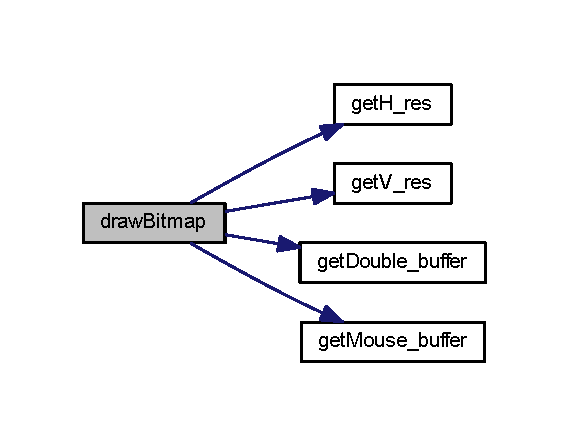
\includegraphics[width=273pt]{group___bitmap_ga18d05a1c671f4638bc63d37874efb9d4_cgraph}
\end{center}
\end{figure}
\hypertarget{group___bitmap_ga3506880ffd407c36eb8aaddd2c1606d2}{}\label{group___bitmap_ga3506880ffd407c36eb8aaddd2c1606d2} 
\index{Bitmap@{Bitmap}!load\+Bitmap@{load\+Bitmap}}
\index{load\+Bitmap@{load\+Bitmap}!Bitmap@{Bitmap}}
\subsubsection{\texorpdfstring{load\+Bitmap()}{loadBitmap()}}
{\footnotesize\ttfamily \hyperlink{struct_bitmap}{Bitmap}$\ast$ load\+Bitmap (\begin{DoxyParamCaption}\item[{const char $\ast$}]{filename }\end{DoxyParamCaption})}



Loads a bmp image. 


\begin{DoxyParams}{Parameters}
{\em filename} & Path of the image to load \\
\hline
\end{DoxyParams}
\begin{DoxyReturn}{Returns}
Non N\+U\+LL pointer to the image buffer
\end{DoxyReturn}
Code from Henrique Ferrolho \href{http://difusal.blogspot.pt/2014/09/minixtutorial-8-loading-bmp-images.html}{\tt http\+://difusal.\+blogspot.\+pt/2014/09/minixtutorial-\/8-\/loading-\/bmp-\/images.\+html} I made some changes in the function draw\+Bitmap The original one drew the \hyperlink{struct_bitmap}{Bitmap} directly in the video\+\_\+mem, whereas the new function draws the \hyperlink{struct_bitmap}{Bitmap} in the double\+\_\+buffer and in the mouse\+\_\+buffer but not on the video\+\_\+mem 

\subsection{Variable Documentation}
\hypertarget{group___bitmap_ga586c4bcc42cf22a033e8f60f24f627f0}{}\label{group___bitmap_ga586c4bcc42cf22a033e8f60f24f627f0} 
\index{Bitmap@{Bitmap}!bitmap\+Data@{bitmap\+Data}}
\index{bitmap\+Data@{bitmap\+Data}!Bitmap@{Bitmap}}
\subsubsection{\texorpdfstring{bitmap\+Data}{bitmapData}}
{\footnotesize\ttfamily unsigned char$\ast$ bitmap\+Data}

\hypertarget{group___bitmap_ga7157ca7f3ce4be47481c472fafd89313}{}\label{group___bitmap_ga7157ca7f3ce4be47481c472fafd89313} 
\index{Bitmap@{Bitmap}!bitmap\+Info\+Header@{bitmap\+Info\+Header}}
\index{bitmap\+Info\+Header@{bitmap\+Info\+Header}!Bitmap@{Bitmap}}
\subsubsection{\texorpdfstring{bitmap\+Info\+Header}{bitmapInfoHeader}}
{\footnotesize\ttfamily \hyperlink{struct_bitmap_info_header}{Bitmap\+Info\+Header} bitmap\+Info\+Header}

\hypertarget{group___bitmap_ga47d1d4d776f8fd3bb0f7dbc3c5aeb534}{}\label{group___bitmap_ga47d1d4d776f8fd3bb0f7dbc3c5aeb534} 
\index{Bitmap@{Bitmap}!bits@{bits}}
\index{bits@{bits}!Bitmap@{Bitmap}}
\subsubsection{\texorpdfstring{bits}{bits}}
{\footnotesize\ttfamily unsigned short bits}



specifies the number of bit per pixel 

\hypertarget{group___bitmap_gad180079f62b44e49ec672c9ef6e078b3}{}\label{group___bitmap_gad180079f62b44e49ec672c9ef6e078b3} 
\index{Bitmap@{Bitmap}!compression@{compression}}
\index{compression@{compression}!Bitmap@{Bitmap}}
\subsubsection{\texorpdfstring{compression}{compression}}
{\footnotesize\ttfamily unsigned int compression}



specifies the type of compression 

\hypertarget{group___bitmap_gad12fc34ce789bce6c8a05d8a17138534}{}\label{group___bitmap_gad12fc34ce789bce6c8a05d8a17138534} 
\index{Bitmap@{Bitmap}!height@{height}}
\index{height@{height}!Bitmap@{Bitmap}}
\subsubsection{\texorpdfstring{height}{height}}
{\footnotesize\ttfamily int height}



specifies height in pixels 

\hypertarget{group___bitmap_gadcd57a0168319e747bc8099218d3822c}{}\label{group___bitmap_gadcd57a0168319e747bc8099218d3822c} 
\index{Bitmap@{Bitmap}!image\+Size@{image\+Size}}
\index{image\+Size@{image\+Size}!Bitmap@{Bitmap}}
\subsubsection{\texorpdfstring{image\+Size}{imageSize}}
{\footnotesize\ttfamily unsigned int image\+Size}



size of image in bytes 

\hypertarget{group___bitmap_ga8f7abfbc446b12f385d2b42c3b4fd9b0}{}\label{group___bitmap_ga8f7abfbc446b12f385d2b42c3b4fd9b0} 
\index{Bitmap@{Bitmap}!important\+Colors@{important\+Colors}}
\index{important\+Colors@{important\+Colors}!Bitmap@{Bitmap}}
\subsubsection{\texorpdfstring{important\+Colors}{importantColors}}
{\footnotesize\ttfamily unsigned int important\+Colors}



number of colors that are important 

\hypertarget{group___bitmap_gaed4506bad904845183194f199f1bdb98}{}\label{group___bitmap_gaed4506bad904845183194f199f1bdb98} 
\index{Bitmap@{Bitmap}!n\+Colors@{n\+Colors}}
\index{n\+Colors@{n\+Colors}!Bitmap@{Bitmap}}
\subsubsection{\texorpdfstring{n\+Colors}{nColors}}
{\footnotesize\ttfamily unsigned int n\+Colors}



number of colors used by the bitmap 

\hypertarget{group___bitmap_ga29b5297d3393519050e3126c4cb07c1c}{}\label{group___bitmap_ga29b5297d3393519050e3126c4cb07c1c} 
\index{Bitmap@{Bitmap}!offset@{offset}}
\index{offset@{offset}!Bitmap@{Bitmap}}
\subsubsection{\texorpdfstring{offset}{offset}}
{\footnotesize\ttfamily unsigned int offset}



specifies the offset in bytes from the bitmapfileheader to the bitmap bits 

\hypertarget{group___bitmap_ga8c89d091e05544a82dc2398eed99634f}{}\label{group___bitmap_ga8c89d091e05544a82dc2398eed99634f} 
\index{Bitmap@{Bitmap}!planes@{planes}}
\index{planes@{planes}!Bitmap@{Bitmap}}
\subsubsection{\texorpdfstring{planes}{planes}}
{\footnotesize\ttfamily unsigned short planes}



specifies the number of color planes, must be 1 

\hypertarget{group___bitmap_ga05d5cbcb44f437341bd9fa37d589aced}{}\label{group___bitmap_ga05d5cbcb44f437341bd9fa37d589aced} 
\index{Bitmap@{Bitmap}!reserved@{reserved}}
\index{reserved@{reserved}!Bitmap@{Bitmap}}
\subsubsection{\texorpdfstring{reserved}{reserved}}
{\footnotesize\ttfamily unsigned int reserved}



reserved; must be 0 

\hypertarget{group___bitmap_gaac913b3a1f6ef005d66bf7a84428773e}{}\label{group___bitmap_gaac913b3a1f6ef005d66bf7a84428773e} 
\index{Bitmap@{Bitmap}!size@{size}}
\index{size@{size}!Bitmap@{Bitmap}}
\subsubsection{\texorpdfstring{size}{size}\hspace{0.1cm}{\footnotesize\ttfamily [1/2]}}
{\footnotesize\ttfamily unsigned int size}



specifies the size in bytes of the bitmap file 

\hypertarget{group___bitmap_gaac913b3a1f6ef005d66bf7a84428773e}{}\label{group___bitmap_gaac913b3a1f6ef005d66bf7a84428773e} 
\index{Bitmap@{Bitmap}!size@{size}}
\index{size@{size}!Bitmap@{Bitmap}}
\subsubsection{\texorpdfstring{size}{size}\hspace{0.1cm}{\footnotesize\ttfamily [2/2]}}
{\footnotesize\ttfamily unsigned int size}



specifies the number of bytes required by the struct 

\hypertarget{group___bitmap_gaa929142c5ddf34cf0915c97a617a1a63}{}\label{group___bitmap_gaa929142c5ddf34cf0915c97a617a1a63} 
\index{Bitmap@{Bitmap}!type@{type}}
\index{type@{type}!Bitmap@{Bitmap}}
\subsubsection{\texorpdfstring{type}{type}}
{\footnotesize\ttfamily unsigned short type}



specifies the file type 

\hypertarget{group___bitmap_ga2474a5474cbff19523a51eb1de01cda4}{}\label{group___bitmap_ga2474a5474cbff19523a51eb1de01cda4} 
\index{Bitmap@{Bitmap}!width@{width}}
\index{width@{width}!Bitmap@{Bitmap}}
\subsubsection{\texorpdfstring{width}{width}}
{\footnotesize\ttfamily int width}



specifies width in pixels 

\hypertarget{group___bitmap_gac6eaeb4c0876cf6cd899f41fe3c25ff5}{}\label{group___bitmap_gac6eaeb4c0876cf6cd899f41fe3c25ff5} 
\index{Bitmap@{Bitmap}!x\+Resolution@{x\+Resolution}}
\index{x\+Resolution@{x\+Resolution}!Bitmap@{Bitmap}}
\subsubsection{\texorpdfstring{x\+Resolution}{xResolution}}
{\footnotesize\ttfamily int x\+Resolution}



number of pixels per meter in x axis 

\hypertarget{group___bitmap_gaa2f350dd0bda750656d5db5f5e37b2b3}{}\label{group___bitmap_gaa2f350dd0bda750656d5db5f5e37b2b3} 
\index{Bitmap@{Bitmap}!y\+Resolution@{y\+Resolution}}
\index{y\+Resolution@{y\+Resolution}!Bitmap@{Bitmap}}
\subsubsection{\texorpdfstring{y\+Resolution}{yResolution}}
{\footnotesize\ttfamily int y\+Resolution}



number of pixels per meter in y axis 


\hypertarget{group___checkers}{}\section{Checkers}
\label{group___checkers}\index{Checkers@{Checkers}}
\subsection*{Data Structures}
\begin{DoxyCompactItemize}
\item 
struct \hyperlink{structmouse__t}{mouse\+\_\+t}
\end{DoxyCompactItemize}
\subsection*{Macros}
\begin{DoxyCompactItemize}
\item 
\#define \hyperlink{group___checkers_ga2f705e070c4925daee2fda4016de437f}{C\+H\+E\+C\+K\+E\+R\+S\+\_\+\+T\+I\+M\+E\+O\+UT}~30
\item 
\#define \hyperlink{group___checkers_ga455c619153ef283f338157e6b2156179}{W\+H\+I\+T\+E\+\_\+\+C\+LR}~0x\+F\+F\+FF
\item 
\#define \hyperlink{group___checkers_ga84d1df2a2deef34e0e9f8d4375b5b8f6}{B\+L\+A\+C\+K\+\_\+\+C\+LR}~0
\item 
\#define \hyperlink{group___checkers_gaaf27b1edff1c7d7a5bf0a59ecb27cb5d}{B\+O\+A\+R\+D\+\_\+\+XI}~320
\item 
\#define \hyperlink{group___checkers_gaea13da4098bc5828bb6b3f6febcfd904}{B\+O\+A\+R\+D\+\_\+\+YI}~192
\item 
\#define \hyperlink{group___checkers_gae49255d26a5f626f705a0ab09f3f2fb8}{B\+O\+A\+R\+D\+\_\+\+S\+Q\+\_\+\+S\+I\+ZE}~80
\item 
\#define \hyperlink{group___checkers_ga0db4eef7cbfb2b192b09094169ce388f}{B\+O\+A\+R\+D\+\_\+\+C\+L\+\_\+\+R\+A\+D\+I\+US}~32
\item 
\#define \hyperlink{group___checkers_ga63f26b52fc35e2f57f2212dd1478d076}{B\+O\+A\+R\+D\+\_\+\+E\+V\+E\+N\+\_\+\+S\+Q\+\_\+\+C\+LR}~0x\+C618
\item 
\#define \hyperlink{group___checkers_ga07198a5ebf1a6ac88de94970f135a8ba}{B\+O\+A\+R\+D\+\_\+\+O\+D\+D\+\_\+\+S\+Q\+\_\+\+C\+LR}~0x18\+C9
\item 
\#define \hyperlink{group___checkers_ga0d38fb3c6c1987840ddb97f7696d997d}{B\+O\+A\+R\+D\+\_\+\+P\+L1\+\_\+\+C\+L\+\_\+\+C\+LR}~0x\+E\+E\+C4
\begin{DoxyCompactList}\small\item\em E8\+D820. \end{DoxyCompactList}\item 
\#define \hyperlink{group___checkers_gaf7041b1453aa70a12d1dac1602d93ca8}{B\+O\+A\+R\+D\+\_\+\+P\+L2\+\_\+\+C\+L\+\_\+\+C\+LR}~0x\+C945
\begin{DoxyCompactList}\small\item\em C82828. \end{DoxyCompactList}\item 
\#define \hyperlink{group___checkers_gaab1a3cc5eb6c2a45aca8a4d8a5e08707}{M\+O\+U\+S\+E\+\_\+\+T\+R\+A\+N\+S\+P\+A\+R\+E\+N\+T\+\_\+\+C\+LR}~0x\+F81F
\item 
\#define \hyperlink{group___checkers_gaa2ef662fb61ca6849a43030a495c4afa}{M\+O\+U\+S\+E\+\_\+\+T\+R\+A\+N\+S\+P\+A\+R\+E\+N\+T\+\_\+\+C\+L\+R\+\_\+2}~0x0001
\item 
\#define \hyperlink{group___checkers_gac55bb8c3d7fd471107553465b14fae49}{T\+U\+R\+N\+\_\+\+M\+S\+G\+\_\+\+C\+LR}~0x1383
\item 
\#define \hyperlink{group___checkers_ga6d237f394788ef28deeaf21d0a6637f2}{T\+U\+R\+N\+\_\+\+M\+S\+G\+\_\+\+Y\+E\+L\+L\+O\+W\+\_\+\+B\+A\+C\+K\+G\+R\+O\+U\+N\+D\+\_\+\+C\+LR}~0x\+E6\+A5
\item 
\#define \hyperlink{group___checkers_ga98c171a878c38e1c25fb081562041c44}{T\+U\+R\+N\+\_\+\+M\+S\+G\+\_\+\+R\+E\+D\+\_\+\+B\+A\+C\+K\+G\+R\+O\+U\+N\+D\+\_\+\+C\+LR}~0x\+C146
\item 
\#define \hyperlink{group___checkers_gaf92e8ff13dda8277eaf67d6a59863510}{T\+U\+R\+N\+\_\+\+M\+S\+G\+\_\+\+X\+I\+\_\+\+R\+ED}~540
\item 
\#define \hyperlink{group___checkers_gae8d1a563a8d7003deca2e08f762ae9f7}{T\+U\+R\+N\+\_\+\+M\+S\+G\+\_\+\+X\+I\+\_\+\+Y\+E\+L\+L\+OW}~480
\item 
\#define \hyperlink{group___checkers_gad96cfcfb473995338b12290370836079}{T\+U\+R\+N\+\_\+\+M\+S\+G\+\_\+\+YI}~100
\end{DoxyCompactItemize}
\subsection*{Enumerations}
\begin{DoxyCompactItemize}
\item 
enum \{ \hyperlink{group___checkers_gga06fc87d81c62e9abb8790b6e5713c55bacad03968ad3abc8b7121ad472826aca9}{S\+T\+A\+T\+E\+\_\+1\+\_\+\+H\+O\+L\+D\+\_\+\+P\+I\+E\+CE}, 
\hyperlink{group___checkers_gga06fc87d81c62e9abb8790b6e5713c55bad88d91bd9763e878df21645bae0ba9b5}{S\+T\+A\+T\+E\+\_\+1\+\_\+\+D\+E\+F\+A\+U\+LT}, 
\hyperlink{group___checkers_gga06fc87d81c62e9abb8790b6e5713c55ba946a863b3f5d8ac63feb55f4e0866597}{S\+T\+A\+T\+E\+\_\+2\+\_\+\+H\+O\+L\+D\+\_\+\+P\+I\+E\+CE}, 
\hyperlink{group___checkers_gga06fc87d81c62e9abb8790b6e5713c55ba156b7cbfed5b8a1ad54b568ebc257ae9}{S\+T\+A\+T\+E\+\_\+2\+\_\+\+D\+E\+F\+A\+U\+LT}
 \}
\end{DoxyCompactItemize}
\subsection*{Functions}
\begin{DoxyCompactItemize}
\item 
int \hyperlink{group___checkers_gad95d8a331ab0758ace223ea301a57f7f}{checkers\+\_\+start\+\_\+game} (char $\ast$path\+\_\+images, int player\+\_\+1, int player\+\_\+2)
\begin{DoxyCompactList}\small\item\em loads the images and starts the game \end{DoxyCompactList}\item 
int \hyperlink{group___checkers_gaf1aa642150939b8b1d104fe437a9d135}{checkers\+\_\+serial\+\_\+handler} (int player\+\_\+1, int player\+\_\+2)
\begin{DoxyCompactList}\small\item\em handles the game in serial mode being responsible for handling which player should play \end{DoxyCompactList}\item 
int \hyperlink{group___checkers_ga61f35c6c9bba94dcd5028e185f3ae3f6}{checkers\+\_\+int\+\_\+handler} (int player1, int player2)
\begin{DoxyCompactList}\small\item\em handles the interrupts \end{DoxyCompactList}\item 
int \hyperlink{group___checkers_gac38396bd73b19b176b4016524f63f8aa}{checkers\+\_\+move\+\_\+handler} (\hyperlink{structmouse__packet__t}{mouse\+\_\+packet\+\_\+t} packet, int player1, int player2)
\begin{DoxyCompactList}\small\item\em handles the moves \end{DoxyCompactList}\item 
int \hyperlink{group___checkers_gac0cf60fd44a44bbb1a7c9ff7ec0d998b}{send\+\_\+serial\+\_\+move} (int player, int xi, int yi, int xf, int yf)
\begin{DoxyCompactList}\small\item\em Sends a message saying that a player did a move. \end{DoxyCompactList}\item 
int \hyperlink{group___checkers_gaa082b9cac17a99c54ac6fa5ac40c660d}{send\+\_\+serial\+\_\+ret} (int r)
\begin{DoxyCompactList}\small\item\em sends a serial message saying that a player finished making a move with the corresponding return value \end{DoxyCompactList}\item 
int \hyperlink{group___checkers_ga17180b891d06475062d87e08d01af278}{wait\+\_\+for\+\_\+serial\+\_\+message} (int player, int $\ast$r, int $\ast$xi, int $\ast$yi, int $\ast$xf, int $\ast$yf)
\begin{DoxyCompactList}\small\item\em Waits for a message from the serial port. \end{DoxyCompactList}\item 
int \hyperlink{group___checkers_gaa6a495a94944bda567df909f84c62396}{draw\+\_\+board} ()
\begin{DoxyCompactList}\small\item\em draws a board on the screen \end{DoxyCompactList}\item 
int \hyperlink{group___checkers_gaf3fd6677c55727d50220875a0031230b}{put\+\_\+square} (int board\+\_\+x, int board\+\_\+y, int color)
\begin{DoxyCompactList}\small\item\em places an empty square \end{DoxyCompactList}\item 
int \hyperlink{group___checkers_ga1d2d36062ce4e9fcdba43dfdc59215d0}{put\+\_\+circle} (int board\+\_\+x, int board\+\_\+y, int color)
\begin{DoxyCompactList}\small\item\em places a circle \end{DoxyCompactList}\item 
int \hyperlink{group___checkers_gaa0642fe5ef48cc14ab51722047092f1f}{move\+\_\+piece} (int player, int xi, int yi, int xf, int yf)
\begin{DoxyCompactList}\small\item\em moves a piece and handles everything pertinent related to the move \end{DoxyCompactList}\item 
int \hyperlink{group___checkers_ga01bdfba712e2ceab4902f5cd63f6b482}{draw\+\_\+turn\+\_\+message} (int x, int y, unsigned int background\+\_\+clr, \hyperlink{struct_bitmap}{Bitmap} $\ast$turn)
\begin{DoxyCompactList}\small\item\em draws the turn message that says who should play now \end{DoxyCompactList}\item 
int \hyperlink{group___checkers_gae4a0f98e772d41a53d13748a7d9d1252}{coord\+\_\+to\+\_\+real\+\_\+board} (int coord\+\_\+x, int coord\+\_\+y, int $\ast$board\+\_\+x, int $\ast$board\+\_\+y)
\begin{DoxyCompactList}\small\item\em converts screen coordinates to board coordinates \end{DoxyCompactList}\item 
int \hyperlink{group___checkers_gad7f7feb83c536c88d67834e7e20780ee}{state\+\_\+to\+\_\+player} (int \hyperlink{checkers_8c_a89f234133d3efe315836311cbf21c64b}{state})
\begin{DoxyCompactList}\small\item\em converts a state to the corresponding player \end{DoxyCompactList}\item 
int \hyperlink{group___checkers_ga258c52e2e4a6ef24d9fb5ec06bedaa53}{create\+\_\+mouse} (int x, int y)
\item 
int \hyperlink{group___checkers_ga597f43aacf586aacf3c32664944f8ba9}{move\+\_\+mouse} (int x\+\_\+delta, int y\+\_\+delta)
\begin{DoxyCompactList}\small\item\em moves mouse (x\+\_\+delta, y\+\_\+delta) \end{DoxyCompactList}\item 
int \hyperlink{group___checkers_ga0f9d87b0bea416d794ed80855026d550}{draw\+\_\+mouse} ()
\begin{DoxyCompactList}\small\item\em draws a mouse \end{DoxyCompactList}\item 
int \hyperlink{group___checkers_ga0580c6365cfa09e2d8a30d3d47f3adb1}{draw\+\_\+mouse\+\_\+circle} (int xi, int yi, int radius, int color)
\begin{DoxyCompactList}\small\item\em draws the the mouse circle \end{DoxyCompactList}\end{DoxyCompactItemize}


\subsection{Detailed Description}
Functions for construction and manipulation of the board 

\subsection{Macro Definition Documentation}
\hypertarget{group___checkers_ga84d1df2a2deef34e0e9f8d4375b5b8f6}{}\label{group___checkers_ga84d1df2a2deef34e0e9f8d4375b5b8f6} 
\index{Checkers@{Checkers}!B\+L\+A\+C\+K\+\_\+\+C\+LR@{B\+L\+A\+C\+K\+\_\+\+C\+LR}}
\index{B\+L\+A\+C\+K\+\_\+\+C\+LR@{B\+L\+A\+C\+K\+\_\+\+C\+LR}!Checkers@{Checkers}}
\subsubsection{\texorpdfstring{B\+L\+A\+C\+K\+\_\+\+C\+LR}{BLACK\_CLR}}
{\footnotesize\ttfamily \#define B\+L\+A\+C\+K\+\_\+\+C\+LR~0}

\hypertarget{group___checkers_ga0db4eef7cbfb2b192b09094169ce388f}{}\label{group___checkers_ga0db4eef7cbfb2b192b09094169ce388f} 
\index{Checkers@{Checkers}!B\+O\+A\+R\+D\+\_\+\+C\+L\+\_\+\+R\+A\+D\+I\+US@{B\+O\+A\+R\+D\+\_\+\+C\+L\+\_\+\+R\+A\+D\+I\+US}}
\index{B\+O\+A\+R\+D\+\_\+\+C\+L\+\_\+\+R\+A\+D\+I\+US@{B\+O\+A\+R\+D\+\_\+\+C\+L\+\_\+\+R\+A\+D\+I\+US}!Checkers@{Checkers}}
\subsubsection{\texorpdfstring{B\+O\+A\+R\+D\+\_\+\+C\+L\+\_\+\+R\+A\+D\+I\+US}{BOARD\_CL\_RADIUS}}
{\footnotesize\ttfamily \#define B\+O\+A\+R\+D\+\_\+\+C\+L\+\_\+\+R\+A\+D\+I\+US~32}

\hypertarget{group___checkers_ga63f26b52fc35e2f57f2212dd1478d076}{}\label{group___checkers_ga63f26b52fc35e2f57f2212dd1478d076} 
\index{Checkers@{Checkers}!B\+O\+A\+R\+D\+\_\+\+E\+V\+E\+N\+\_\+\+S\+Q\+\_\+\+C\+LR@{B\+O\+A\+R\+D\+\_\+\+E\+V\+E\+N\+\_\+\+S\+Q\+\_\+\+C\+LR}}
\index{B\+O\+A\+R\+D\+\_\+\+E\+V\+E\+N\+\_\+\+S\+Q\+\_\+\+C\+LR@{B\+O\+A\+R\+D\+\_\+\+E\+V\+E\+N\+\_\+\+S\+Q\+\_\+\+C\+LR}!Checkers@{Checkers}}
\subsubsection{\texorpdfstring{B\+O\+A\+R\+D\+\_\+\+E\+V\+E\+N\+\_\+\+S\+Q\+\_\+\+C\+LR}{BOARD\_EVEN\_SQ\_CLR}}
{\footnotesize\ttfamily \#define B\+O\+A\+R\+D\+\_\+\+E\+V\+E\+N\+\_\+\+S\+Q\+\_\+\+C\+LR~0x\+C618}

\hypertarget{group___checkers_ga07198a5ebf1a6ac88de94970f135a8ba}{}\label{group___checkers_ga07198a5ebf1a6ac88de94970f135a8ba} 
\index{Checkers@{Checkers}!B\+O\+A\+R\+D\+\_\+\+O\+D\+D\+\_\+\+S\+Q\+\_\+\+C\+LR@{B\+O\+A\+R\+D\+\_\+\+O\+D\+D\+\_\+\+S\+Q\+\_\+\+C\+LR}}
\index{B\+O\+A\+R\+D\+\_\+\+O\+D\+D\+\_\+\+S\+Q\+\_\+\+C\+LR@{B\+O\+A\+R\+D\+\_\+\+O\+D\+D\+\_\+\+S\+Q\+\_\+\+C\+LR}!Checkers@{Checkers}}
\subsubsection{\texorpdfstring{B\+O\+A\+R\+D\+\_\+\+O\+D\+D\+\_\+\+S\+Q\+\_\+\+C\+LR}{BOARD\_ODD\_SQ\_CLR}}
{\footnotesize\ttfamily \#define B\+O\+A\+R\+D\+\_\+\+O\+D\+D\+\_\+\+S\+Q\+\_\+\+C\+LR~0x18\+C9}

\hypertarget{group___checkers_ga0d38fb3c6c1987840ddb97f7696d997d}{}\label{group___checkers_ga0d38fb3c6c1987840ddb97f7696d997d} 
\index{Checkers@{Checkers}!B\+O\+A\+R\+D\+\_\+\+P\+L1\+\_\+\+C\+L\+\_\+\+C\+LR@{B\+O\+A\+R\+D\+\_\+\+P\+L1\+\_\+\+C\+L\+\_\+\+C\+LR}}
\index{B\+O\+A\+R\+D\+\_\+\+P\+L1\+\_\+\+C\+L\+\_\+\+C\+LR@{B\+O\+A\+R\+D\+\_\+\+P\+L1\+\_\+\+C\+L\+\_\+\+C\+LR}!Checkers@{Checkers}}
\subsubsection{\texorpdfstring{B\+O\+A\+R\+D\+\_\+\+P\+L1\+\_\+\+C\+L\+\_\+\+C\+LR}{BOARD\_PL1\_CL\_CLR}}
{\footnotesize\ttfamily \#define B\+O\+A\+R\+D\+\_\+\+P\+L1\+\_\+\+C\+L\+\_\+\+C\+LR~0x\+E\+E\+C4}



E8\+D820. 

\hypertarget{group___checkers_gaf7041b1453aa70a12d1dac1602d93ca8}{}\label{group___checkers_gaf7041b1453aa70a12d1dac1602d93ca8} 
\index{Checkers@{Checkers}!B\+O\+A\+R\+D\+\_\+\+P\+L2\+\_\+\+C\+L\+\_\+\+C\+LR@{B\+O\+A\+R\+D\+\_\+\+P\+L2\+\_\+\+C\+L\+\_\+\+C\+LR}}
\index{B\+O\+A\+R\+D\+\_\+\+P\+L2\+\_\+\+C\+L\+\_\+\+C\+LR@{B\+O\+A\+R\+D\+\_\+\+P\+L2\+\_\+\+C\+L\+\_\+\+C\+LR}!Checkers@{Checkers}}
\subsubsection{\texorpdfstring{B\+O\+A\+R\+D\+\_\+\+P\+L2\+\_\+\+C\+L\+\_\+\+C\+LR}{BOARD\_PL2\_CL\_CLR}}
{\footnotesize\ttfamily \#define B\+O\+A\+R\+D\+\_\+\+P\+L2\+\_\+\+C\+L\+\_\+\+C\+LR~0x\+C945}



C82828. 

\hypertarget{group___checkers_gae49255d26a5f626f705a0ab09f3f2fb8}{}\label{group___checkers_gae49255d26a5f626f705a0ab09f3f2fb8} 
\index{Checkers@{Checkers}!B\+O\+A\+R\+D\+\_\+\+S\+Q\+\_\+\+S\+I\+ZE@{B\+O\+A\+R\+D\+\_\+\+S\+Q\+\_\+\+S\+I\+ZE}}
\index{B\+O\+A\+R\+D\+\_\+\+S\+Q\+\_\+\+S\+I\+ZE@{B\+O\+A\+R\+D\+\_\+\+S\+Q\+\_\+\+S\+I\+ZE}!Checkers@{Checkers}}
\subsubsection{\texorpdfstring{B\+O\+A\+R\+D\+\_\+\+S\+Q\+\_\+\+S\+I\+ZE}{BOARD\_SQ\_SIZE}}
{\footnotesize\ttfamily \#define B\+O\+A\+R\+D\+\_\+\+S\+Q\+\_\+\+S\+I\+ZE~80}

\hypertarget{group___checkers_gaaf27b1edff1c7d7a5bf0a59ecb27cb5d}{}\label{group___checkers_gaaf27b1edff1c7d7a5bf0a59ecb27cb5d} 
\index{Checkers@{Checkers}!B\+O\+A\+R\+D\+\_\+\+XI@{B\+O\+A\+R\+D\+\_\+\+XI}}
\index{B\+O\+A\+R\+D\+\_\+\+XI@{B\+O\+A\+R\+D\+\_\+\+XI}!Checkers@{Checkers}}
\subsubsection{\texorpdfstring{B\+O\+A\+R\+D\+\_\+\+XI}{BOARD\_XI}}
{\footnotesize\ttfamily \#define B\+O\+A\+R\+D\+\_\+\+XI~320}

\hypertarget{group___checkers_gaea13da4098bc5828bb6b3f6febcfd904}{}\label{group___checkers_gaea13da4098bc5828bb6b3f6febcfd904} 
\index{Checkers@{Checkers}!B\+O\+A\+R\+D\+\_\+\+YI@{B\+O\+A\+R\+D\+\_\+\+YI}}
\index{B\+O\+A\+R\+D\+\_\+\+YI@{B\+O\+A\+R\+D\+\_\+\+YI}!Checkers@{Checkers}}
\subsubsection{\texorpdfstring{B\+O\+A\+R\+D\+\_\+\+YI}{BOARD\_YI}}
{\footnotesize\ttfamily \#define B\+O\+A\+R\+D\+\_\+\+YI~192}

\hypertarget{group___checkers_ga2f705e070c4925daee2fda4016de437f}{}\label{group___checkers_ga2f705e070c4925daee2fda4016de437f} 
\index{Checkers@{Checkers}!C\+H\+E\+C\+K\+E\+R\+S\+\_\+\+T\+I\+M\+E\+O\+UT@{C\+H\+E\+C\+K\+E\+R\+S\+\_\+\+T\+I\+M\+E\+O\+UT}}
\index{C\+H\+E\+C\+K\+E\+R\+S\+\_\+\+T\+I\+M\+E\+O\+UT@{C\+H\+E\+C\+K\+E\+R\+S\+\_\+\+T\+I\+M\+E\+O\+UT}!Checkers@{Checkers}}
\subsubsection{\texorpdfstring{C\+H\+E\+C\+K\+E\+R\+S\+\_\+\+T\+I\+M\+E\+O\+UT}{CHECKERS\_TIMEOUT}}
{\footnotesize\ttfamily \#define C\+H\+E\+C\+K\+E\+R\+S\+\_\+\+T\+I\+M\+E\+O\+UT~30}

\hypertarget{group___checkers_gaab1a3cc5eb6c2a45aca8a4d8a5e08707}{}\label{group___checkers_gaab1a3cc5eb6c2a45aca8a4d8a5e08707} 
\index{Checkers@{Checkers}!M\+O\+U\+S\+E\+\_\+\+T\+R\+A\+N\+S\+P\+A\+R\+E\+N\+T\+\_\+\+C\+LR@{M\+O\+U\+S\+E\+\_\+\+T\+R\+A\+N\+S\+P\+A\+R\+E\+N\+T\+\_\+\+C\+LR}}
\index{M\+O\+U\+S\+E\+\_\+\+T\+R\+A\+N\+S\+P\+A\+R\+E\+N\+T\+\_\+\+C\+LR@{M\+O\+U\+S\+E\+\_\+\+T\+R\+A\+N\+S\+P\+A\+R\+E\+N\+T\+\_\+\+C\+LR}!Checkers@{Checkers}}
\subsubsection{\texorpdfstring{M\+O\+U\+S\+E\+\_\+\+T\+R\+A\+N\+S\+P\+A\+R\+E\+N\+T\+\_\+\+C\+LR}{MOUSE\_TRANSPARENT\_CLR}}
{\footnotesize\ttfamily \#define M\+O\+U\+S\+E\+\_\+\+T\+R\+A\+N\+S\+P\+A\+R\+E\+N\+T\+\_\+\+C\+LR~0x\+F81F}

\hypertarget{group___checkers_gaa2ef662fb61ca6849a43030a495c4afa}{}\label{group___checkers_gaa2ef662fb61ca6849a43030a495c4afa} 
\index{Checkers@{Checkers}!M\+O\+U\+S\+E\+\_\+\+T\+R\+A\+N\+S\+P\+A\+R\+E\+N\+T\+\_\+\+C\+L\+R\+\_\+2@{M\+O\+U\+S\+E\+\_\+\+T\+R\+A\+N\+S\+P\+A\+R\+E\+N\+T\+\_\+\+C\+L\+R\+\_\+2}}
\index{M\+O\+U\+S\+E\+\_\+\+T\+R\+A\+N\+S\+P\+A\+R\+E\+N\+T\+\_\+\+C\+L\+R\+\_\+2@{M\+O\+U\+S\+E\+\_\+\+T\+R\+A\+N\+S\+P\+A\+R\+E\+N\+T\+\_\+\+C\+L\+R\+\_\+2}!Checkers@{Checkers}}
\subsubsection{\texorpdfstring{M\+O\+U\+S\+E\+\_\+\+T\+R\+A\+N\+S\+P\+A\+R\+E\+N\+T\+\_\+\+C\+L\+R\+\_\+2}{MOUSE\_TRANSPARENT\_CLR\_2}}
{\footnotesize\ttfamily \#define M\+O\+U\+S\+E\+\_\+\+T\+R\+A\+N\+S\+P\+A\+R\+E\+N\+T\+\_\+\+C\+L\+R\+\_\+2~0x0001}

\hypertarget{group___checkers_gac55bb8c3d7fd471107553465b14fae49}{}\label{group___checkers_gac55bb8c3d7fd471107553465b14fae49} 
\index{Checkers@{Checkers}!T\+U\+R\+N\+\_\+\+M\+S\+G\+\_\+\+C\+LR@{T\+U\+R\+N\+\_\+\+M\+S\+G\+\_\+\+C\+LR}}
\index{T\+U\+R\+N\+\_\+\+M\+S\+G\+\_\+\+C\+LR@{T\+U\+R\+N\+\_\+\+M\+S\+G\+\_\+\+C\+LR}!Checkers@{Checkers}}
\subsubsection{\texorpdfstring{T\+U\+R\+N\+\_\+\+M\+S\+G\+\_\+\+C\+LR}{TURN\_MSG\_CLR}}
{\footnotesize\ttfamily \#define T\+U\+R\+N\+\_\+\+M\+S\+G\+\_\+\+C\+LR~0x1383}

\hypertarget{group___checkers_ga98c171a878c38e1c25fb081562041c44}{}\label{group___checkers_ga98c171a878c38e1c25fb081562041c44} 
\index{Checkers@{Checkers}!T\+U\+R\+N\+\_\+\+M\+S\+G\+\_\+\+R\+E\+D\+\_\+\+B\+A\+C\+K\+G\+R\+O\+U\+N\+D\+\_\+\+C\+LR@{T\+U\+R\+N\+\_\+\+M\+S\+G\+\_\+\+R\+E\+D\+\_\+\+B\+A\+C\+K\+G\+R\+O\+U\+N\+D\+\_\+\+C\+LR}}
\index{T\+U\+R\+N\+\_\+\+M\+S\+G\+\_\+\+R\+E\+D\+\_\+\+B\+A\+C\+K\+G\+R\+O\+U\+N\+D\+\_\+\+C\+LR@{T\+U\+R\+N\+\_\+\+M\+S\+G\+\_\+\+R\+E\+D\+\_\+\+B\+A\+C\+K\+G\+R\+O\+U\+N\+D\+\_\+\+C\+LR}!Checkers@{Checkers}}
\subsubsection{\texorpdfstring{T\+U\+R\+N\+\_\+\+M\+S\+G\+\_\+\+R\+E\+D\+\_\+\+B\+A\+C\+K\+G\+R\+O\+U\+N\+D\+\_\+\+C\+LR}{TURN\_MSG\_RED\_BACKGROUND\_CLR}}
{\footnotesize\ttfamily \#define T\+U\+R\+N\+\_\+\+M\+S\+G\+\_\+\+R\+E\+D\+\_\+\+B\+A\+C\+K\+G\+R\+O\+U\+N\+D\+\_\+\+C\+LR~0x\+C146}

\hypertarget{group___checkers_gaf92e8ff13dda8277eaf67d6a59863510}{}\label{group___checkers_gaf92e8ff13dda8277eaf67d6a59863510} 
\index{Checkers@{Checkers}!T\+U\+R\+N\+\_\+\+M\+S\+G\+\_\+\+X\+I\+\_\+\+R\+ED@{T\+U\+R\+N\+\_\+\+M\+S\+G\+\_\+\+X\+I\+\_\+\+R\+ED}}
\index{T\+U\+R\+N\+\_\+\+M\+S\+G\+\_\+\+X\+I\+\_\+\+R\+ED@{T\+U\+R\+N\+\_\+\+M\+S\+G\+\_\+\+X\+I\+\_\+\+R\+ED}!Checkers@{Checkers}}
\subsubsection{\texorpdfstring{T\+U\+R\+N\+\_\+\+M\+S\+G\+\_\+\+X\+I\+\_\+\+R\+ED}{TURN\_MSG\_XI\_RED}}
{\footnotesize\ttfamily \#define T\+U\+R\+N\+\_\+\+M\+S\+G\+\_\+\+X\+I\+\_\+\+R\+ED~540}

\hypertarget{group___checkers_gae8d1a563a8d7003deca2e08f762ae9f7}{}\label{group___checkers_gae8d1a563a8d7003deca2e08f762ae9f7} 
\index{Checkers@{Checkers}!T\+U\+R\+N\+\_\+\+M\+S\+G\+\_\+\+X\+I\+\_\+\+Y\+E\+L\+L\+OW@{T\+U\+R\+N\+\_\+\+M\+S\+G\+\_\+\+X\+I\+\_\+\+Y\+E\+L\+L\+OW}}
\index{T\+U\+R\+N\+\_\+\+M\+S\+G\+\_\+\+X\+I\+\_\+\+Y\+E\+L\+L\+OW@{T\+U\+R\+N\+\_\+\+M\+S\+G\+\_\+\+X\+I\+\_\+\+Y\+E\+L\+L\+OW}!Checkers@{Checkers}}
\subsubsection{\texorpdfstring{T\+U\+R\+N\+\_\+\+M\+S\+G\+\_\+\+X\+I\+\_\+\+Y\+E\+L\+L\+OW}{TURN\_MSG\_XI\_YELLOW}}
{\footnotesize\ttfamily \#define T\+U\+R\+N\+\_\+\+M\+S\+G\+\_\+\+X\+I\+\_\+\+Y\+E\+L\+L\+OW~480}

\hypertarget{group___checkers_ga6d237f394788ef28deeaf21d0a6637f2}{}\label{group___checkers_ga6d237f394788ef28deeaf21d0a6637f2} 
\index{Checkers@{Checkers}!T\+U\+R\+N\+\_\+\+M\+S\+G\+\_\+\+Y\+E\+L\+L\+O\+W\+\_\+\+B\+A\+C\+K\+G\+R\+O\+U\+N\+D\+\_\+\+C\+LR@{T\+U\+R\+N\+\_\+\+M\+S\+G\+\_\+\+Y\+E\+L\+L\+O\+W\+\_\+\+B\+A\+C\+K\+G\+R\+O\+U\+N\+D\+\_\+\+C\+LR}}
\index{T\+U\+R\+N\+\_\+\+M\+S\+G\+\_\+\+Y\+E\+L\+L\+O\+W\+\_\+\+B\+A\+C\+K\+G\+R\+O\+U\+N\+D\+\_\+\+C\+LR@{T\+U\+R\+N\+\_\+\+M\+S\+G\+\_\+\+Y\+E\+L\+L\+O\+W\+\_\+\+B\+A\+C\+K\+G\+R\+O\+U\+N\+D\+\_\+\+C\+LR}!Checkers@{Checkers}}
\subsubsection{\texorpdfstring{T\+U\+R\+N\+\_\+\+M\+S\+G\+\_\+\+Y\+E\+L\+L\+O\+W\+\_\+\+B\+A\+C\+K\+G\+R\+O\+U\+N\+D\+\_\+\+C\+LR}{TURN\_MSG\_YELLOW\_BACKGROUND\_CLR}}
{\footnotesize\ttfamily \#define T\+U\+R\+N\+\_\+\+M\+S\+G\+\_\+\+Y\+E\+L\+L\+O\+W\+\_\+\+B\+A\+C\+K\+G\+R\+O\+U\+N\+D\+\_\+\+C\+LR~0x\+E6\+A5}

\hypertarget{group___checkers_gad96cfcfb473995338b12290370836079}{}\label{group___checkers_gad96cfcfb473995338b12290370836079} 
\index{Checkers@{Checkers}!T\+U\+R\+N\+\_\+\+M\+S\+G\+\_\+\+YI@{T\+U\+R\+N\+\_\+\+M\+S\+G\+\_\+\+YI}}
\index{T\+U\+R\+N\+\_\+\+M\+S\+G\+\_\+\+YI@{T\+U\+R\+N\+\_\+\+M\+S\+G\+\_\+\+YI}!Checkers@{Checkers}}
\subsubsection{\texorpdfstring{T\+U\+R\+N\+\_\+\+M\+S\+G\+\_\+\+YI}{TURN\_MSG\_YI}}
{\footnotesize\ttfamily \#define T\+U\+R\+N\+\_\+\+M\+S\+G\+\_\+\+YI~100}

\hypertarget{group___checkers_ga455c619153ef283f338157e6b2156179}{}\label{group___checkers_ga455c619153ef283f338157e6b2156179} 
\index{Checkers@{Checkers}!W\+H\+I\+T\+E\+\_\+\+C\+LR@{W\+H\+I\+T\+E\+\_\+\+C\+LR}}
\index{W\+H\+I\+T\+E\+\_\+\+C\+LR@{W\+H\+I\+T\+E\+\_\+\+C\+LR}!Checkers@{Checkers}}
\subsubsection{\texorpdfstring{W\+H\+I\+T\+E\+\_\+\+C\+LR}{WHITE\_CLR}}
{\footnotesize\ttfamily \#define W\+H\+I\+T\+E\+\_\+\+C\+LR~0x\+F\+F\+FF}



\subsection{Enumeration Type Documentation}
\hypertarget{group___checkers_ga06fc87d81c62e9abb8790b6e5713c55b}{}\label{group___checkers_ga06fc87d81c62e9abb8790b6e5713c55b} 
\subsubsection{\texorpdfstring{anonymous enum}{anonymous enum}}
{\footnotesize\ttfamily anonymous enum}

States of the game \begin{DoxyEnumFields}{Enumerator}
\raisebox{\heightof{T}}[0pt][0pt]{\index{S\+T\+A\+T\+E\+\_\+1\+\_\+\+H\+O\+L\+D\+\_\+\+P\+I\+E\+CE@{S\+T\+A\+T\+E\+\_\+1\+\_\+\+H\+O\+L\+D\+\_\+\+P\+I\+E\+CE}!Checkers@{Checkers}}\index{Checkers@{Checkers}!S\+T\+A\+T\+E\+\_\+1\+\_\+\+H\+O\+L\+D\+\_\+\+P\+I\+E\+CE@{S\+T\+A\+T\+E\+\_\+1\+\_\+\+H\+O\+L\+D\+\_\+\+P\+I\+E\+CE}}}\hypertarget{group___checkers_gga06fc87d81c62e9abb8790b6e5713c55bacad03968ad3abc8b7121ad472826aca9}{}\label{group___checkers_gga06fc87d81c62e9abb8790b6e5713c55bacad03968ad3abc8b7121ad472826aca9} 
S\+T\+A\+T\+E\+\_\+1\+\_\+\+H\+O\+L\+D\+\_\+\+P\+I\+E\+CE&when player 1 is holding a piece and it\textquotesingle{}s his turn \\
\hline

\raisebox{\heightof{T}}[0pt][0pt]{\index{S\+T\+A\+T\+E\+\_\+1\+\_\+\+D\+E\+F\+A\+U\+LT@{S\+T\+A\+T\+E\+\_\+1\+\_\+\+D\+E\+F\+A\+U\+LT}!Checkers@{Checkers}}\index{Checkers@{Checkers}!S\+T\+A\+T\+E\+\_\+1\+\_\+\+D\+E\+F\+A\+U\+LT@{S\+T\+A\+T\+E\+\_\+1\+\_\+\+D\+E\+F\+A\+U\+LT}}}\hypertarget{group___checkers_gga06fc87d81c62e9abb8790b6e5713c55bad88d91bd9763e878df21645bae0ba9b5}{}\label{group___checkers_gga06fc87d81c62e9abb8790b6e5713c55bad88d91bd9763e878df21645bae0ba9b5} 
S\+T\+A\+T\+E\+\_\+1\+\_\+\+D\+E\+F\+A\+U\+LT&when it\textquotesingle{}s player 1 turn and he is not doing anything \\
\hline

\raisebox{\heightof{T}}[0pt][0pt]{\index{S\+T\+A\+T\+E\+\_\+2\+\_\+\+H\+O\+L\+D\+\_\+\+P\+I\+E\+CE@{S\+T\+A\+T\+E\+\_\+2\+\_\+\+H\+O\+L\+D\+\_\+\+P\+I\+E\+CE}!Checkers@{Checkers}}\index{Checkers@{Checkers}!S\+T\+A\+T\+E\+\_\+2\+\_\+\+H\+O\+L\+D\+\_\+\+P\+I\+E\+CE@{S\+T\+A\+T\+E\+\_\+2\+\_\+\+H\+O\+L\+D\+\_\+\+P\+I\+E\+CE}}}\hypertarget{group___checkers_gga06fc87d81c62e9abb8790b6e5713c55ba946a863b3f5d8ac63feb55f4e0866597}{}\label{group___checkers_gga06fc87d81c62e9abb8790b6e5713c55ba946a863b3f5d8ac63feb55f4e0866597} 
S\+T\+A\+T\+E\+\_\+2\+\_\+\+H\+O\+L\+D\+\_\+\+P\+I\+E\+CE&when player 2 is holding a piece and it\textquotesingle{}s his turn \\
\hline

\raisebox{\heightof{T}}[0pt][0pt]{\index{S\+T\+A\+T\+E\+\_\+2\+\_\+\+D\+E\+F\+A\+U\+LT@{S\+T\+A\+T\+E\+\_\+2\+\_\+\+D\+E\+F\+A\+U\+LT}!Checkers@{Checkers}}\index{Checkers@{Checkers}!S\+T\+A\+T\+E\+\_\+2\+\_\+\+D\+E\+F\+A\+U\+LT@{S\+T\+A\+T\+E\+\_\+2\+\_\+\+D\+E\+F\+A\+U\+LT}}}\hypertarget{group___checkers_gga06fc87d81c62e9abb8790b6e5713c55ba156b7cbfed5b8a1ad54b568ebc257ae9}{}\label{group___checkers_gga06fc87d81c62e9abb8790b6e5713c55ba156b7cbfed5b8a1ad54b568ebc257ae9} 
S\+T\+A\+T\+E\+\_\+2\+\_\+\+D\+E\+F\+A\+U\+LT&when it\textquotesingle{}s player 2 turn and he is not doing anything \\
\hline

\end{DoxyEnumFields}


\subsection{Function Documentation}
\hypertarget{group___checkers_ga61f35c6c9bba94dcd5028e185f3ae3f6}{}\label{group___checkers_ga61f35c6c9bba94dcd5028e185f3ae3f6} 
\index{Checkers@{Checkers}!checkers\+\_\+int\+\_\+handler@{checkers\+\_\+int\+\_\+handler}}
\index{checkers\+\_\+int\+\_\+handler@{checkers\+\_\+int\+\_\+handler}!Checkers@{Checkers}}
\subsubsection{\texorpdfstring{checkers\+\_\+int\+\_\+handler()}{checkers\_int\_handler()}}
{\footnotesize\ttfamily int checkers\+\_\+int\+\_\+handler (\begin{DoxyParamCaption}\item[{int}]{player1,  }\item[{int}]{player2 }\end{DoxyParamCaption})}



handles the interrupts 


\begin{DoxyParams}{Parameters}
{\em player\+\_\+1} & set to 1 if player\+\_\+1 is currently playing, o otherwise \\
\hline
{\em player\+\_\+2} & set to 1 if player\+\_\+2 is currently playing \\
\hline
\end{DoxyParams}
\begin{DoxyReturn}{Returns}
1 in case of success, 0 otherwise 
\end{DoxyReturn}
Here is the call graph for this function\+:
% FIG 0
\hypertarget{group___checkers_gac38396bd73b19b176b4016524f63f8aa}{}\label{group___checkers_gac38396bd73b19b176b4016524f63f8aa} 
\index{Checkers@{Checkers}!checkers\+\_\+move\+\_\+handler@{checkers\+\_\+move\+\_\+handler}}
\index{checkers\+\_\+move\+\_\+handler@{checkers\+\_\+move\+\_\+handler}!Checkers@{Checkers}}
\subsubsection{\texorpdfstring{checkers\+\_\+move\+\_\+handler()}{checkers\_move\_handler()}}
{\footnotesize\ttfamily int checkers\+\_\+move\+\_\+handler (\begin{DoxyParamCaption}\item[{\hyperlink{structmouse__packet__t}{mouse\+\_\+packet\+\_\+t}}]{packet,  }\item[{int}]{player1,  }\item[{int}]{player2 }\end{DoxyParamCaption})}



handles the moves 


\begin{DoxyParams}{Parameters}
{\em player\+\_\+1} & set to 1 if player\+\_\+1 is currently playing, o otherwise \\
\hline
{\em player\+\_\+2} & set to 1 if player\+\_\+2 is currently playing \\
\hline
\end{DoxyParams}
\begin{DoxyReturn}{Returns}
1 in case of success, 0 otherwise 
\end{DoxyReturn}
Here is the call graph for this function\+:
% FIG 1
\hypertarget{group___checkers_gaf1aa642150939b8b1d104fe437a9d135}{}\label{group___checkers_gaf1aa642150939b8b1d104fe437a9d135} 
\index{Checkers@{Checkers}!checkers\+\_\+serial\+\_\+handler@{checkers\+\_\+serial\+\_\+handler}}
\index{checkers\+\_\+serial\+\_\+handler@{checkers\+\_\+serial\+\_\+handler}!Checkers@{Checkers}}
\subsubsection{\texorpdfstring{checkers\+\_\+serial\+\_\+handler()}{checkers\_serial\_handler()}}
{\footnotesize\ttfamily int checkers\+\_\+serial\+\_\+handler (\begin{DoxyParamCaption}\item[{int}]{player\+\_\+1,  }\item[{int}]{player\+\_\+2 }\end{DoxyParamCaption})}



handles the game in serial mode being responsible for handling which player should play 


\begin{DoxyParams}{Parameters}
{\em player\+\_\+1} & set to 1 if player\+\_\+1 is currently playing, o otherwise \\
\hline
{\em player\+\_\+2} & set to 1 if player\+\_\+2 is currently playing \\
\hline
\end{DoxyParams}
\begin{DoxyReturn}{Returns}
1 in case of success, 0 otherwise 
\end{DoxyReturn}
Here is the call graph for this function\+:
% FIG 2
\hypertarget{group___checkers_gad95d8a331ab0758ace223ea301a57f7f}{}\label{group___checkers_gad95d8a331ab0758ace223ea301a57f7f} 
\index{Checkers@{Checkers}!checkers\+\_\+start\+\_\+game@{checkers\+\_\+start\+\_\+game}}
\index{checkers\+\_\+start\+\_\+game@{checkers\+\_\+start\+\_\+game}!Checkers@{Checkers}}
\subsubsection{\texorpdfstring{checkers\+\_\+start\+\_\+game()}{checkers\_start\_game()}}
{\footnotesize\ttfamily int checkers\+\_\+start\+\_\+game (\begin{DoxyParamCaption}\item[{char $\ast$}]{path\+\_\+images,  }\item[{int}]{player\+\_\+1,  }\item[{int}]{player\+\_\+2 }\end{DoxyParamCaption})}



loads the images and starts the game 


\begin{DoxyParams}{Parameters}
{\em path\+\_\+images} & path of y«the directory that the contains the images \\
\hline
{\em player\+\_\+1} & set to 1 if player\+\_\+1 is currently playing, o otherwise \\
\hline
{\em player\+\_\+2} & set to 1 if player\+\_\+2 is currently playing \\
\hline
\end{DoxyParams}
\begin{DoxyReturn}{Returns}
1 in case of success, 0 otherwise 
\end{DoxyReturn}
Here is the call graph for this function\+:
% FIG 3
\hypertarget{group___checkers_gae4a0f98e772d41a53d13748a7d9d1252}{}\label{group___checkers_gae4a0f98e772d41a53d13748a7d9d1252} 
\index{Checkers@{Checkers}!coord\+\_\+to\+\_\+real\+\_\+board@{coord\+\_\+to\+\_\+real\+\_\+board}}
\index{coord\+\_\+to\+\_\+real\+\_\+board@{coord\+\_\+to\+\_\+real\+\_\+board}!Checkers@{Checkers}}
\subsubsection{\texorpdfstring{coord\+\_\+to\+\_\+real\+\_\+board()}{coord\_to\_real\_board()}}
{\footnotesize\ttfamily int coord\+\_\+to\+\_\+real\+\_\+board (\begin{DoxyParamCaption}\item[{int}]{coord\+\_\+x,  }\item[{int}]{coord\+\_\+y,  }\item[{int $\ast$}]{board\+\_\+x,  }\item[{int $\ast$}]{board\+\_\+y }\end{DoxyParamCaption})}



converts screen coordinates to board coordinates 


\begin{DoxyParams}{Parameters}
{\em coord\+\_\+x} & screen coordinate x \\
\hline
{\em coord\+\_\+y} & screen coordinate y \\
\hline
{\em board\+\_\+x} & board coordinate x \\
\hline
{\em board\+\_\+y} & board coordinate y \\
\hline
\end{DoxyParams}
\begin{DoxyReturn}{Returns}
0 in case of success, 1 otherwise 
\end{DoxyReturn}
\hypertarget{group___checkers_ga258c52e2e4a6ef24d9fb5ec06bedaa53}{}\label{group___checkers_ga258c52e2e4a6ef24d9fb5ec06bedaa53} 
\index{Checkers@{Checkers}!create\+\_\+mouse@{create\+\_\+mouse}}
\index{create\+\_\+mouse@{create\+\_\+mouse}!Checkers@{Checkers}}
\subsubsection{\texorpdfstring{create\+\_\+mouse()}{create\_mouse()}}
{\footnotesize\ttfamily int create\+\_\+mouse (\begin{DoxyParamCaption}\item[{int}]{x,  }\item[{int}]{y }\end{DoxyParamCaption})}

\hypertarget{group___checkers_gaa6a495a94944bda567df909f84c62396}{}\label{group___checkers_gaa6a495a94944bda567df909f84c62396} 
\index{Checkers@{Checkers}!draw\+\_\+board@{draw\+\_\+board}}
\index{draw\+\_\+board@{draw\+\_\+board}!Checkers@{Checkers}}
\subsubsection{\texorpdfstring{draw\+\_\+board()}{draw\_board()}}
{\footnotesize\ttfamily int draw\+\_\+board (\begin{DoxyParamCaption}{ }\end{DoxyParamCaption})}



draws a board on the screen 

\begin{DoxyReturn}{Returns}
1 in case of success, 0 otherwise 
\end{DoxyReturn}
Here is the call graph for this function\+:
% FIG 4
\hypertarget{group___checkers_ga0f9d87b0bea416d794ed80855026d550}{}\label{group___checkers_ga0f9d87b0bea416d794ed80855026d550} 
\index{Checkers@{Checkers}!draw\+\_\+mouse@{draw\+\_\+mouse}}
\index{draw\+\_\+mouse@{draw\+\_\+mouse}!Checkers@{Checkers}}
\subsubsection{\texorpdfstring{draw\+\_\+mouse()}{draw\_mouse()}}
{\footnotesize\ttfamily int draw\+\_\+mouse (\begin{DoxyParamCaption}{ }\end{DoxyParamCaption})}



draws a mouse 

Here is the call graph for this function\+:
% FIG 5
\hypertarget{group___checkers_ga0580c6365cfa09e2d8a30d3d47f3adb1}{}\label{group___checkers_ga0580c6365cfa09e2d8a30d3d47f3adb1} 
\index{Checkers@{Checkers}!draw\+\_\+mouse\+\_\+circle@{draw\+\_\+mouse\+\_\+circle}}
\index{draw\+\_\+mouse\+\_\+circle@{draw\+\_\+mouse\+\_\+circle}!Checkers@{Checkers}}
\subsubsection{\texorpdfstring{draw\+\_\+mouse\+\_\+circle()}{draw\_mouse\_circle()}}
{\footnotesize\ttfamily int draw\+\_\+mouse\+\_\+circle (\begin{DoxyParamCaption}\item[{int}]{xi,  }\item[{int}]{yi,  }\item[{int}]{radius,  }\item[{int}]{color }\end{DoxyParamCaption})}



draws the the mouse circle 

Here is the call graph for this function\+:
% FIG 6
\hypertarget{group___checkers_ga01bdfba712e2ceab4902f5cd63f6b482}{}\label{group___checkers_ga01bdfba712e2ceab4902f5cd63f6b482} 
\index{Checkers@{Checkers}!draw\+\_\+turn\+\_\+message@{draw\+\_\+turn\+\_\+message}}
\index{draw\+\_\+turn\+\_\+message@{draw\+\_\+turn\+\_\+message}!Checkers@{Checkers}}
\subsubsection{\texorpdfstring{draw\+\_\+turn\+\_\+message()}{draw\_turn\_message()}}
{\footnotesize\ttfamily int draw\+\_\+turn\+\_\+message (\begin{DoxyParamCaption}\item[{int}]{x,  }\item[{int}]{y,  }\item[{unsigned int}]{background\+\_\+clr,  }\item[{\hyperlink{struct_bitmap}{Bitmap} $\ast$}]{turn }\end{DoxyParamCaption})}



draws the turn message that says who should play now 

Here is the call graph for this function\+:
% FIG 7
\hypertarget{group___checkers_ga597f43aacf586aacf3c32664944f8ba9}{}\label{group___checkers_ga597f43aacf586aacf3c32664944f8ba9} 
\index{Checkers@{Checkers}!move\+\_\+mouse@{move\+\_\+mouse}}
\index{move\+\_\+mouse@{move\+\_\+mouse}!Checkers@{Checkers}}
\subsubsection{\texorpdfstring{move\+\_\+mouse()}{move\_mouse()}}
{\footnotesize\ttfamily int move\+\_\+mouse (\begin{DoxyParamCaption}\item[{int}]{x\+\_\+delta,  }\item[{int}]{y\+\_\+delta }\end{DoxyParamCaption})}



moves mouse (x\+\_\+delta, y\+\_\+delta) 

Here is the call graph for this function\+:
% FIG 8
\hypertarget{group___checkers_gaa0642fe5ef48cc14ab51722047092f1f}{}\label{group___checkers_gaa0642fe5ef48cc14ab51722047092f1f} 
\index{Checkers@{Checkers}!move\+\_\+piece@{move\+\_\+piece}}
\index{move\+\_\+piece@{move\+\_\+piece}!Checkers@{Checkers}}
\subsubsection{\texorpdfstring{move\+\_\+piece()}{move\_piece()}}
{\footnotesize\ttfamily int move\+\_\+piece (\begin{DoxyParamCaption}\item[{int}]{player,  }\item[{int}]{xi,  }\item[{int}]{yi,  }\item[{int}]{xf,  }\item[{int}]{yf }\end{DoxyParamCaption})}



moves a piece and handles everything pertinent related to the move 


\begin{DoxyParams}{Parameters}
{\em player} & player that made the move \\
\hline
{\em xi} & initial x position \\
\hline
{\em yi} & initial y position \\
\hline
{\em xf} & final x position \\
\hline
{\em yf} & final y position \\
\hline
\end{DoxyParams}
\begin{DoxyReturn}{Returns}
1 in case of success, 0 otherwise 
\end{DoxyReturn}
Here is the call graph for this function\+:
% FIG 9
\hypertarget{group___checkers_ga1d2d36062ce4e9fcdba43dfdc59215d0}{}\label{group___checkers_ga1d2d36062ce4e9fcdba43dfdc59215d0} 
\index{Checkers@{Checkers}!put\+\_\+circle@{put\+\_\+circle}}
\index{put\+\_\+circle@{put\+\_\+circle}!Checkers@{Checkers}}
\subsubsection{\texorpdfstring{put\+\_\+circle()}{put\_circle()}}
{\footnotesize\ttfamily int put\+\_\+circle (\begin{DoxyParamCaption}\item[{int}]{board\+\_\+x,  }\item[{int}]{board\+\_\+y,  }\item[{int}]{color }\end{DoxyParamCaption})}



places a circle 


\begin{DoxyParams}{Parameters}
{\em board\+\_\+x} & x coordinate \\
\hline
{\em board\+\_\+y} & y coordinate \\
\hline
{\em color} & color of the square \\
\hline
\end{DoxyParams}
\begin{DoxyReturn}{Returns}
0 in case of success, 1 otherwise 
\end{DoxyReturn}
Here is the call graph for this function\+:
% FIG 10
\hypertarget{group___checkers_gaf3fd6677c55727d50220875a0031230b}{}\label{group___checkers_gaf3fd6677c55727d50220875a0031230b} 
\index{Checkers@{Checkers}!put\+\_\+square@{put\+\_\+square}}
\index{put\+\_\+square@{put\+\_\+square}!Checkers@{Checkers}}
\subsubsection{\texorpdfstring{put\+\_\+square()}{put\_square()}}
{\footnotesize\ttfamily int put\+\_\+square (\begin{DoxyParamCaption}\item[{int}]{board\+\_\+x,  }\item[{int}]{board\+\_\+y,  }\item[{int}]{color }\end{DoxyParamCaption})}



places an empty square 


\begin{DoxyParams}{Parameters}
{\em board\+\_\+x} & x coordinate \\
\hline
{\em board\+\_\+y} & y coordinate \\
\hline
{\em color} & color of the square \\
\hline
\end{DoxyParams}
\begin{DoxyReturn}{Returns}
0 in case of success, 1 otherwise 
\end{DoxyReturn}
Here is the call graph for this function\+:
% FIG 11
\hypertarget{group___checkers_gac0cf60fd44a44bbb1a7c9ff7ec0d998b}{}\label{group___checkers_gac0cf60fd44a44bbb1a7c9ff7ec0d998b} 
\index{Checkers@{Checkers}!send\+\_\+serial\+\_\+move@{send\+\_\+serial\+\_\+move}}
\index{send\+\_\+serial\+\_\+move@{send\+\_\+serial\+\_\+move}!Checkers@{Checkers}}
\subsubsection{\texorpdfstring{send\+\_\+serial\+\_\+move()}{send\_serial\_move()}}
{\footnotesize\ttfamily int send\+\_\+serial\+\_\+move (\begin{DoxyParamCaption}\item[{int}]{player,  }\item[{int}]{xi,  }\item[{int}]{yi,  }\item[{int}]{xf,  }\item[{int}]{yf }\end{DoxyParamCaption})}



Sends a message saying that a player did a move. 


\begin{DoxyParams}{Parameters}
{\em player} & player that made the move \\
\hline
{\em xi} & initial x position \\
\hline
{\em yi} & initial y position \\
\hline
{\em xf} & final x position \\
\hline
{\em yf} & final y position \\
\hline
\end{DoxyParams}
\begin{DoxyReturn}{Returns}
1 in case of success, 0 otherwise 
\end{DoxyReturn}
Here is the call graph for this function\+:
% FIG 12
\hypertarget{group___checkers_gaa082b9cac17a99c54ac6fa5ac40c660d}{}\label{group___checkers_gaa082b9cac17a99c54ac6fa5ac40c660d} 
\index{Checkers@{Checkers}!send\+\_\+serial\+\_\+ret@{send\+\_\+serial\+\_\+ret}}
\index{send\+\_\+serial\+\_\+ret@{send\+\_\+serial\+\_\+ret}!Checkers@{Checkers}}
\subsubsection{\texorpdfstring{send\+\_\+serial\+\_\+ret()}{send\_serial\_ret()}}
{\footnotesize\ttfamily int send\+\_\+serial\+\_\+ret (\begin{DoxyParamCaption}\item[{int}]{r }\end{DoxyParamCaption})}



sends a serial message saying that a player finished making a move with the corresponding return value 


\begin{DoxyParams}{Parameters}
{\em r} & return value \\
\hline
\end{DoxyParams}
\begin{DoxyReturn}{Returns}
1 in case of success, 0 otherwise 
\end{DoxyReturn}
Here is the call graph for this function\+:
% FIG 13
\hypertarget{group___checkers_gad7f7feb83c536c88d67834e7e20780ee}{}\label{group___checkers_gad7f7feb83c536c88d67834e7e20780ee} 
\index{Checkers@{Checkers}!state\+\_\+to\+\_\+player@{state\+\_\+to\+\_\+player}}
\index{state\+\_\+to\+\_\+player@{state\+\_\+to\+\_\+player}!Checkers@{Checkers}}
\subsubsection{\texorpdfstring{state\+\_\+to\+\_\+player()}{state\_to\_player()}}
{\footnotesize\ttfamily int state\+\_\+to\+\_\+player (\begin{DoxyParamCaption}\item[{int}]{state }\end{DoxyParamCaption})}



converts a state to the corresponding player 

\hypertarget{group___checkers_ga17180b891d06475062d87e08d01af278}{}\label{group___checkers_ga17180b891d06475062d87e08d01af278} 
\index{Checkers@{Checkers}!wait\+\_\+for\+\_\+serial\+\_\+message@{wait\+\_\+for\+\_\+serial\+\_\+message}}
\index{wait\+\_\+for\+\_\+serial\+\_\+message@{wait\+\_\+for\+\_\+serial\+\_\+message}!Checkers@{Checkers}}
\subsubsection{\texorpdfstring{wait\+\_\+for\+\_\+serial\+\_\+message()}{wait\_for\_serial\_message()}}
{\footnotesize\ttfamily int wait\+\_\+for\+\_\+serial\+\_\+message (\begin{DoxyParamCaption}\item[{int}]{player,  }\item[{int $\ast$}]{r,  }\item[{int $\ast$}]{xi,  }\item[{int $\ast$}]{yi,  }\item[{int $\ast$}]{xf,  }\item[{int $\ast$}]{yf }\end{DoxyParamCaption})}



Waits for a message from the serial port. 


\begin{DoxyParams}{Parameters}
{\em player} & player that is waiting for the message \\
\hline
{\em r} & return value \\
\hline
{\em xi} & initial x position \\
\hline
{\em yi} & initial y position \\
\hline
{\em xf} & final x position \\
\hline
{\em yf} & final y position \\
\hline
\end{DoxyParams}
\begin{DoxyReturn}{Returns}
1 in case of success, 0 otherwise 
\end{DoxyReturn}
Here is the call graph for this function\+:
% FIG 14

\hypertarget{group__i8042}{}\section{i8042}
\label{group__i8042}\index{i8042@{i8042}}
\subsection*{K\+BC}
\begin{DoxyCompactItemize}
\item 
\#define \hyperlink{group__i8042_ga16c5827f043d82f87c726c2d4369c11d}{K\+B\+C\+\_\+\+I\+RQ}~1
\item 
\#define \hyperlink{group__i8042_ga1ccde68b2b6d4e45b50eef1403e10bb7}{K\+B\+C\+\_\+\+O\+U\+T\+\_\+\+B\+UF}~0x60
\item 
\#define \hyperlink{group__i8042_gaac9289c99cf0a693a211da6d6cb1bb65}{K\+B\+C\+\_\+\+I\+N\+\_\+\+B\+UF}~0x60
\item 
\#define \hyperlink{group__i8042_ga34b14687d83496940a236351fbbb1aea}{K\+B\+C\+\_\+\+S\+T\+A\+T\+\_\+\+R\+EG}~0x64
\item 
\#define \hyperlink{group__i8042_ga6d57c7927a10f638c83046b52c8caac9}{K\+B\+C\+\_\+\+C\+M\+D\+\_\+\+R\+EG}~0x64
\item 
\#define \hyperlink{group__i8042_ga7bff22c3c71947a24f8f0922d33f0f5f}{C\+K\+B\+D\+\_\+\+A\+CK}~0xfa
\item 
\#define \hyperlink{group__i8042_gafbc8d3dd7a27e8c020c9991578358def}{C\+K\+B\+D\+\_\+\+R\+E\+S\+E\+ND}~0xfe
\item 
\#define \hyperlink{group__i8042_ga318cf5bf776792ffc02a53fb7e8082df}{C\+K\+B\+D\+\_\+\+E\+R\+R\+OR}~0xfc
\item 
\#define \hyperlink{group__i8042_ga36930de8a703505c95fe133095dcfe06}{K\+B\+C\+\_\+\+O\+BF}~\hyperlink{video__gr_8c_a3a8ea58898cb58fc96013383d39f482c}{B\+IT}(0)
\item 
\#define \hyperlink{group__i8042_gac1649d41f8ba9a02fa70ec4e600d5e4a}{K\+B\+C\+\_\+\+I\+BF}~\hyperlink{video__gr_8c_a3a8ea58898cb58fc96013383d39f482c}{B\+IT}(1)
\item 
\#define \hyperlink{group__i8042_ga795488c410d300a8ea2afb4c82d2e6cc}{K\+B\+C\+\_\+\+P\+A\+R\+\_\+\+E\+R\+R\+OR}~\hyperlink{video__gr_8c_a3a8ea58898cb58fc96013383d39f482c}{B\+IT}(7)
\item 
\#define \hyperlink{group__i8042_ga22767b69efd74d1f3631b8803a63b939}{K\+B\+C\+\_\+\+T\+O\+\_\+\+E\+R\+R\+OR}~\hyperlink{video__gr_8c_a3a8ea58898cb58fc96013383d39f482c}{B\+IT}(6)
\item 
\#define \hyperlink{group__i8042_ga1747d582dc5a6d634f05016ece9625d8}{K\+B\+C\+\_\+\+W\+R\+I\+T\+E\+\_\+\+T\+O\+\_\+\+M\+O\+U\+SE}~0x\+D4
\item 
\#define \hyperlink{group__i8042_gac69c14ded6b68de11e5caaa6bcddf8fc}{K\+B\+D\+\_\+\+L\+E\+DS}~0xed
\item 
\#define \hyperlink{group__i8042_ga1b7a8d18cf6c99a32610259ae861eb1f}{K\+B\+D\+\_\+\+L\+ED}(n)~(1$<$$<$n)
\end{DoxyCompactItemize}
\subsection*{M\+O\+U\+SE}
\begin{DoxyCompactItemize}
\item 
\#define \hyperlink{group__i8042_ga85964cb90343bb1a029b1d1b4229f910}{M\+O\+U\+S\+E\+\_\+\+I\+RQ}~12
\item 
\#define \hyperlink{group__i8042_ga6b902000c4f0a66e57f0eb78d7611105}{M\+O\+U\+S\+E\+\_\+\+R\+E\+S\+ET}~0xff
\item 
\#define \hyperlink{group__i8042_ga094907f521b569f790a760be8885ec4d}{M\+O\+U\+S\+E\+\_\+\+D\+I\+S\+A\+B\+LE}~0xf5
\item 
\#define \hyperlink{group__i8042_ga4e6aa8d10e05b5f94c196bfe2cdfb8d7}{M\+O\+U\+S\+E\+\_\+\+E\+N\+A\+B\+LE}~0xf4
\item 
\#define \hyperlink{group__i8042_gafcda52e19d0d6e3053ec9e51c548254d}{M\+O\+U\+S\+E\+\_\+\+S\+E\+T\+\_\+\+S\+T\+R\+E\+AM}~0xea
\item 
\#define \hyperlink{group__i8042_gadb427fdde0b4b8715e843c54e1ae7522}{M\+O\+U\+S\+E\+\_\+\+D\+I\+S\+A\+B\+L\+E\+\_\+\+S\+T\+R\+E\+A\+M\+\_\+\+M\+O\+DE}~0\+X\+F5
\item 
\#define \hyperlink{group__i8042_gae81dac725cb48935cbc4564c35a46c5d}{M\+O\+U\+S\+E\+\_\+\+S\+T\+A\+T\+U\+S\+\_\+\+R\+E\+Q\+U\+E\+ST}~0x\+E9
\end{DoxyCompactItemize}


\subsection{Detailed Description}
Constants for programming the i8042 controller. 

\subsection{Macro Definition Documentation}
\hypertarget{group__i8042_ga7bff22c3c71947a24f8f0922d33f0f5f}{}\label{group__i8042_ga7bff22c3c71947a24f8f0922d33f0f5f} 
\index{i8042@{i8042}!C\+K\+B\+D\+\_\+\+A\+CK@{C\+K\+B\+D\+\_\+\+A\+CK}}
\index{C\+K\+B\+D\+\_\+\+A\+CK@{C\+K\+B\+D\+\_\+\+A\+CK}!i8042@{i8042}}
\subsubsection{\texorpdfstring{C\+K\+B\+D\+\_\+\+A\+CK}{CKBD\_ACK}}
{\footnotesize\ttfamily \#define C\+K\+B\+D\+\_\+\+A\+CK~0xfa}

\hypertarget{group__i8042_ga318cf5bf776792ffc02a53fb7e8082df}{}\label{group__i8042_ga318cf5bf776792ffc02a53fb7e8082df} 
\index{i8042@{i8042}!C\+K\+B\+D\+\_\+\+E\+R\+R\+OR@{C\+K\+B\+D\+\_\+\+E\+R\+R\+OR}}
\index{C\+K\+B\+D\+\_\+\+E\+R\+R\+OR@{C\+K\+B\+D\+\_\+\+E\+R\+R\+OR}!i8042@{i8042}}
\subsubsection{\texorpdfstring{C\+K\+B\+D\+\_\+\+E\+R\+R\+OR}{CKBD\_ERROR}}
{\footnotesize\ttfamily \#define C\+K\+B\+D\+\_\+\+E\+R\+R\+OR~0xfc}

\hypertarget{group__i8042_gafbc8d3dd7a27e8c020c9991578358def}{}\label{group__i8042_gafbc8d3dd7a27e8c020c9991578358def} 
\index{i8042@{i8042}!C\+K\+B\+D\+\_\+\+R\+E\+S\+E\+ND@{C\+K\+B\+D\+\_\+\+R\+E\+S\+E\+ND}}
\index{C\+K\+B\+D\+\_\+\+R\+E\+S\+E\+ND@{C\+K\+B\+D\+\_\+\+R\+E\+S\+E\+ND}!i8042@{i8042}}
\subsubsection{\texorpdfstring{C\+K\+B\+D\+\_\+\+R\+E\+S\+E\+ND}{CKBD\_RESEND}}
{\footnotesize\ttfamily \#define C\+K\+B\+D\+\_\+\+R\+E\+S\+E\+ND~0xfe}

\hypertarget{group__i8042_ga6d57c7927a10f638c83046b52c8caac9}{}\label{group__i8042_ga6d57c7927a10f638c83046b52c8caac9} 
\index{i8042@{i8042}!K\+B\+C\+\_\+\+C\+M\+D\+\_\+\+R\+EG@{K\+B\+C\+\_\+\+C\+M\+D\+\_\+\+R\+EG}}
\index{K\+B\+C\+\_\+\+C\+M\+D\+\_\+\+R\+EG@{K\+B\+C\+\_\+\+C\+M\+D\+\_\+\+R\+EG}!i8042@{i8042}}
\subsubsection{\texorpdfstring{K\+B\+C\+\_\+\+C\+M\+D\+\_\+\+R\+EG}{KBC\_CMD\_REG}}
{\footnotesize\ttfamily \#define K\+B\+C\+\_\+\+C\+M\+D\+\_\+\+R\+EG~0x64}

\hypertarget{group__i8042_gac1649d41f8ba9a02fa70ec4e600d5e4a}{}\label{group__i8042_gac1649d41f8ba9a02fa70ec4e600d5e4a} 
\index{i8042@{i8042}!K\+B\+C\+\_\+\+I\+BF@{K\+B\+C\+\_\+\+I\+BF}}
\index{K\+B\+C\+\_\+\+I\+BF@{K\+B\+C\+\_\+\+I\+BF}!i8042@{i8042}}
\subsubsection{\texorpdfstring{K\+B\+C\+\_\+\+I\+BF}{KBC\_IBF}}
{\footnotesize\ttfamily \#define K\+B\+C\+\_\+\+I\+BF~\hyperlink{video__gr_8c_a3a8ea58898cb58fc96013383d39f482c}{B\+IT}(1)}

\hypertarget{group__i8042_gaac9289c99cf0a693a211da6d6cb1bb65}{}\label{group__i8042_gaac9289c99cf0a693a211da6d6cb1bb65} 
\index{i8042@{i8042}!K\+B\+C\+\_\+\+I\+N\+\_\+\+B\+UF@{K\+B\+C\+\_\+\+I\+N\+\_\+\+B\+UF}}
\index{K\+B\+C\+\_\+\+I\+N\+\_\+\+B\+UF@{K\+B\+C\+\_\+\+I\+N\+\_\+\+B\+UF}!i8042@{i8042}}
\subsubsection{\texorpdfstring{K\+B\+C\+\_\+\+I\+N\+\_\+\+B\+UF}{KBC\_IN\_BUF}}
{\footnotesize\ttfamily \#define K\+B\+C\+\_\+\+I\+N\+\_\+\+B\+UF~0x60}

\hypertarget{group__i8042_ga16c5827f043d82f87c726c2d4369c11d}{}\label{group__i8042_ga16c5827f043d82f87c726c2d4369c11d} 
\index{i8042@{i8042}!K\+B\+C\+\_\+\+I\+RQ@{K\+B\+C\+\_\+\+I\+RQ}}
\index{K\+B\+C\+\_\+\+I\+RQ@{K\+B\+C\+\_\+\+I\+RQ}!i8042@{i8042}}
\subsubsection{\texorpdfstring{K\+B\+C\+\_\+\+I\+RQ}{KBC\_IRQ}}
{\footnotesize\ttfamily \#define K\+B\+C\+\_\+\+I\+RQ~1}

\hypertarget{group__i8042_ga36930de8a703505c95fe133095dcfe06}{}\label{group__i8042_ga36930de8a703505c95fe133095dcfe06} 
\index{i8042@{i8042}!K\+B\+C\+\_\+\+O\+BF@{K\+B\+C\+\_\+\+O\+BF}}
\index{K\+B\+C\+\_\+\+O\+BF@{K\+B\+C\+\_\+\+O\+BF}!i8042@{i8042}}
\subsubsection{\texorpdfstring{K\+B\+C\+\_\+\+O\+BF}{KBC\_OBF}}
{\footnotesize\ttfamily \#define K\+B\+C\+\_\+\+O\+BF~\hyperlink{video__gr_8c_a3a8ea58898cb58fc96013383d39f482c}{B\+IT}(0)}

\hypertarget{group__i8042_ga1ccde68b2b6d4e45b50eef1403e10bb7}{}\label{group__i8042_ga1ccde68b2b6d4e45b50eef1403e10bb7} 
\index{i8042@{i8042}!K\+B\+C\+\_\+\+O\+U\+T\+\_\+\+B\+UF@{K\+B\+C\+\_\+\+O\+U\+T\+\_\+\+B\+UF}}
\index{K\+B\+C\+\_\+\+O\+U\+T\+\_\+\+B\+UF@{K\+B\+C\+\_\+\+O\+U\+T\+\_\+\+B\+UF}!i8042@{i8042}}
\subsubsection{\texorpdfstring{K\+B\+C\+\_\+\+O\+U\+T\+\_\+\+B\+UF}{KBC\_OUT\_BUF}}
{\footnotesize\ttfamily \#define K\+B\+C\+\_\+\+O\+U\+T\+\_\+\+B\+UF~0x60}

\hypertarget{group__i8042_ga795488c410d300a8ea2afb4c82d2e6cc}{}\label{group__i8042_ga795488c410d300a8ea2afb4c82d2e6cc} 
\index{i8042@{i8042}!K\+B\+C\+\_\+\+P\+A\+R\+\_\+\+E\+R\+R\+OR@{K\+B\+C\+\_\+\+P\+A\+R\+\_\+\+E\+R\+R\+OR}}
\index{K\+B\+C\+\_\+\+P\+A\+R\+\_\+\+E\+R\+R\+OR@{K\+B\+C\+\_\+\+P\+A\+R\+\_\+\+E\+R\+R\+OR}!i8042@{i8042}}
\subsubsection{\texorpdfstring{K\+B\+C\+\_\+\+P\+A\+R\+\_\+\+E\+R\+R\+OR}{KBC\_PAR\_ERROR}}
{\footnotesize\ttfamily \#define K\+B\+C\+\_\+\+P\+A\+R\+\_\+\+E\+R\+R\+OR~\hyperlink{video__gr_8c_a3a8ea58898cb58fc96013383d39f482c}{B\+IT}(7)}

\hypertarget{group__i8042_ga34b14687d83496940a236351fbbb1aea}{}\label{group__i8042_ga34b14687d83496940a236351fbbb1aea} 
\index{i8042@{i8042}!K\+B\+C\+\_\+\+S\+T\+A\+T\+\_\+\+R\+EG@{K\+B\+C\+\_\+\+S\+T\+A\+T\+\_\+\+R\+EG}}
\index{K\+B\+C\+\_\+\+S\+T\+A\+T\+\_\+\+R\+EG@{K\+B\+C\+\_\+\+S\+T\+A\+T\+\_\+\+R\+EG}!i8042@{i8042}}
\subsubsection{\texorpdfstring{K\+B\+C\+\_\+\+S\+T\+A\+T\+\_\+\+R\+EG}{KBC\_STAT\_REG}}
{\footnotesize\ttfamily \#define K\+B\+C\+\_\+\+S\+T\+A\+T\+\_\+\+R\+EG~0x64}

\hypertarget{group__i8042_ga22767b69efd74d1f3631b8803a63b939}{}\label{group__i8042_ga22767b69efd74d1f3631b8803a63b939} 
\index{i8042@{i8042}!K\+B\+C\+\_\+\+T\+O\+\_\+\+E\+R\+R\+OR@{K\+B\+C\+\_\+\+T\+O\+\_\+\+E\+R\+R\+OR}}
\index{K\+B\+C\+\_\+\+T\+O\+\_\+\+E\+R\+R\+OR@{K\+B\+C\+\_\+\+T\+O\+\_\+\+E\+R\+R\+OR}!i8042@{i8042}}
\subsubsection{\texorpdfstring{K\+B\+C\+\_\+\+T\+O\+\_\+\+E\+R\+R\+OR}{KBC\_TO\_ERROR}}
{\footnotesize\ttfamily \#define K\+B\+C\+\_\+\+T\+O\+\_\+\+E\+R\+R\+OR~\hyperlink{video__gr_8c_a3a8ea58898cb58fc96013383d39f482c}{B\+IT}(6)}

\hypertarget{group__i8042_ga1747d582dc5a6d634f05016ece9625d8}{}\label{group__i8042_ga1747d582dc5a6d634f05016ece9625d8} 
\index{i8042@{i8042}!K\+B\+C\+\_\+\+W\+R\+I\+T\+E\+\_\+\+T\+O\+\_\+\+M\+O\+U\+SE@{K\+B\+C\+\_\+\+W\+R\+I\+T\+E\+\_\+\+T\+O\+\_\+\+M\+O\+U\+SE}}
\index{K\+B\+C\+\_\+\+W\+R\+I\+T\+E\+\_\+\+T\+O\+\_\+\+M\+O\+U\+SE@{K\+B\+C\+\_\+\+W\+R\+I\+T\+E\+\_\+\+T\+O\+\_\+\+M\+O\+U\+SE}!i8042@{i8042}}
\subsubsection{\texorpdfstring{K\+B\+C\+\_\+\+W\+R\+I\+T\+E\+\_\+\+T\+O\+\_\+\+M\+O\+U\+SE}{KBC\_WRITE\_TO\_MOUSE}}
{\footnotesize\ttfamily \#define K\+B\+C\+\_\+\+W\+R\+I\+T\+E\+\_\+\+T\+O\+\_\+\+M\+O\+U\+SE~0x\+D4}

\hypertarget{group__i8042_ga1b7a8d18cf6c99a32610259ae861eb1f}{}\label{group__i8042_ga1b7a8d18cf6c99a32610259ae861eb1f} 
\index{i8042@{i8042}!K\+B\+D\+\_\+\+L\+ED@{K\+B\+D\+\_\+\+L\+ED}}
\index{K\+B\+D\+\_\+\+L\+ED@{K\+B\+D\+\_\+\+L\+ED}!i8042@{i8042}}
\subsubsection{\texorpdfstring{K\+B\+D\+\_\+\+L\+ED}{KBD\_LED}}
{\footnotesize\ttfamily \#define K\+B\+D\+\_\+\+L\+ED(\begin{DoxyParamCaption}\item[{}]{n }\end{DoxyParamCaption})~(1$<$$<$n)}

\hypertarget{group__i8042_gac69c14ded6b68de11e5caaa6bcddf8fc}{}\label{group__i8042_gac69c14ded6b68de11e5caaa6bcddf8fc} 
\index{i8042@{i8042}!K\+B\+D\+\_\+\+L\+E\+DS@{K\+B\+D\+\_\+\+L\+E\+DS}}
\index{K\+B\+D\+\_\+\+L\+E\+DS@{K\+B\+D\+\_\+\+L\+E\+DS}!i8042@{i8042}}
\subsubsection{\texorpdfstring{K\+B\+D\+\_\+\+L\+E\+DS}{KBD\_LEDS}}
{\footnotesize\ttfamily \#define K\+B\+D\+\_\+\+L\+E\+DS~0xed}

\hypertarget{group__i8042_ga094907f521b569f790a760be8885ec4d}{}\label{group__i8042_ga094907f521b569f790a760be8885ec4d} 
\index{i8042@{i8042}!M\+O\+U\+S\+E\+\_\+\+D\+I\+S\+A\+B\+LE@{M\+O\+U\+S\+E\+\_\+\+D\+I\+S\+A\+B\+LE}}
\index{M\+O\+U\+S\+E\+\_\+\+D\+I\+S\+A\+B\+LE@{M\+O\+U\+S\+E\+\_\+\+D\+I\+S\+A\+B\+LE}!i8042@{i8042}}
\subsubsection{\texorpdfstring{M\+O\+U\+S\+E\+\_\+\+D\+I\+S\+A\+B\+LE}{MOUSE\_DISABLE}}
{\footnotesize\ttfamily \#define M\+O\+U\+S\+E\+\_\+\+D\+I\+S\+A\+B\+LE~0xf5}

\hypertarget{group__i8042_gadb427fdde0b4b8715e843c54e1ae7522}{}\label{group__i8042_gadb427fdde0b4b8715e843c54e1ae7522} 
\index{i8042@{i8042}!M\+O\+U\+S\+E\+\_\+\+D\+I\+S\+A\+B\+L\+E\+\_\+\+S\+T\+R\+E\+A\+M\+\_\+\+M\+O\+DE@{M\+O\+U\+S\+E\+\_\+\+D\+I\+S\+A\+B\+L\+E\+\_\+\+S\+T\+R\+E\+A\+M\+\_\+\+M\+O\+DE}}
\index{M\+O\+U\+S\+E\+\_\+\+D\+I\+S\+A\+B\+L\+E\+\_\+\+S\+T\+R\+E\+A\+M\+\_\+\+M\+O\+DE@{M\+O\+U\+S\+E\+\_\+\+D\+I\+S\+A\+B\+L\+E\+\_\+\+S\+T\+R\+E\+A\+M\+\_\+\+M\+O\+DE}!i8042@{i8042}}
\subsubsection{\texorpdfstring{M\+O\+U\+S\+E\+\_\+\+D\+I\+S\+A\+B\+L\+E\+\_\+\+S\+T\+R\+E\+A\+M\+\_\+\+M\+O\+DE}{MOUSE\_DISABLE\_STREAM\_MODE}}
{\footnotesize\ttfamily \#define M\+O\+U\+S\+E\+\_\+\+D\+I\+S\+A\+B\+L\+E\+\_\+\+S\+T\+R\+E\+A\+M\+\_\+\+M\+O\+DE~0\+X\+F5}

\hypertarget{group__i8042_ga4e6aa8d10e05b5f94c196bfe2cdfb8d7}{}\label{group__i8042_ga4e6aa8d10e05b5f94c196bfe2cdfb8d7} 
\index{i8042@{i8042}!M\+O\+U\+S\+E\+\_\+\+E\+N\+A\+B\+LE@{M\+O\+U\+S\+E\+\_\+\+E\+N\+A\+B\+LE}}
\index{M\+O\+U\+S\+E\+\_\+\+E\+N\+A\+B\+LE@{M\+O\+U\+S\+E\+\_\+\+E\+N\+A\+B\+LE}!i8042@{i8042}}
\subsubsection{\texorpdfstring{M\+O\+U\+S\+E\+\_\+\+E\+N\+A\+B\+LE}{MOUSE\_ENABLE}}
{\footnotesize\ttfamily \#define M\+O\+U\+S\+E\+\_\+\+E\+N\+A\+B\+LE~0xf4}

\hypertarget{group__i8042_ga85964cb90343bb1a029b1d1b4229f910}{}\label{group__i8042_ga85964cb90343bb1a029b1d1b4229f910} 
\index{i8042@{i8042}!M\+O\+U\+S\+E\+\_\+\+I\+RQ@{M\+O\+U\+S\+E\+\_\+\+I\+RQ}}
\index{M\+O\+U\+S\+E\+\_\+\+I\+RQ@{M\+O\+U\+S\+E\+\_\+\+I\+RQ}!i8042@{i8042}}
\subsubsection{\texorpdfstring{M\+O\+U\+S\+E\+\_\+\+I\+RQ}{MOUSE\_IRQ}}
{\footnotesize\ttfamily \#define M\+O\+U\+S\+E\+\_\+\+I\+RQ~12}

\hypertarget{group__i8042_ga6b902000c4f0a66e57f0eb78d7611105}{}\label{group__i8042_ga6b902000c4f0a66e57f0eb78d7611105} 
\index{i8042@{i8042}!M\+O\+U\+S\+E\+\_\+\+R\+E\+S\+ET@{M\+O\+U\+S\+E\+\_\+\+R\+E\+S\+ET}}
\index{M\+O\+U\+S\+E\+\_\+\+R\+E\+S\+ET@{M\+O\+U\+S\+E\+\_\+\+R\+E\+S\+ET}!i8042@{i8042}}
\subsubsection{\texorpdfstring{M\+O\+U\+S\+E\+\_\+\+R\+E\+S\+ET}{MOUSE\_RESET}}
{\footnotesize\ttfamily \#define M\+O\+U\+S\+E\+\_\+\+R\+E\+S\+ET~0xff}

\hypertarget{group__i8042_gafcda52e19d0d6e3053ec9e51c548254d}{}\label{group__i8042_gafcda52e19d0d6e3053ec9e51c548254d} 
\index{i8042@{i8042}!M\+O\+U\+S\+E\+\_\+\+S\+E\+T\+\_\+\+S\+T\+R\+E\+AM@{M\+O\+U\+S\+E\+\_\+\+S\+E\+T\+\_\+\+S\+T\+R\+E\+AM}}
\index{M\+O\+U\+S\+E\+\_\+\+S\+E\+T\+\_\+\+S\+T\+R\+E\+AM@{M\+O\+U\+S\+E\+\_\+\+S\+E\+T\+\_\+\+S\+T\+R\+E\+AM}!i8042@{i8042}}
\subsubsection{\texorpdfstring{M\+O\+U\+S\+E\+\_\+\+S\+E\+T\+\_\+\+S\+T\+R\+E\+AM}{MOUSE\_SET\_STREAM}}
{\footnotesize\ttfamily \#define M\+O\+U\+S\+E\+\_\+\+S\+E\+T\+\_\+\+S\+T\+R\+E\+AM~0xea}

\hypertarget{group__i8042_gae81dac725cb48935cbc4564c35a46c5d}{}\label{group__i8042_gae81dac725cb48935cbc4564c35a46c5d} 
\index{i8042@{i8042}!M\+O\+U\+S\+E\+\_\+\+S\+T\+A\+T\+U\+S\+\_\+\+R\+E\+Q\+U\+E\+ST@{M\+O\+U\+S\+E\+\_\+\+S\+T\+A\+T\+U\+S\+\_\+\+R\+E\+Q\+U\+E\+ST}}
\index{M\+O\+U\+S\+E\+\_\+\+S\+T\+A\+T\+U\+S\+\_\+\+R\+E\+Q\+U\+E\+ST@{M\+O\+U\+S\+E\+\_\+\+S\+T\+A\+T\+U\+S\+\_\+\+R\+E\+Q\+U\+E\+ST}!i8042@{i8042}}
\subsubsection{\texorpdfstring{M\+O\+U\+S\+E\+\_\+\+S\+T\+A\+T\+U\+S\+\_\+\+R\+E\+Q\+U\+E\+ST}{MOUSE\_STATUS\_REQUEST}}
{\footnotesize\ttfamily \#define M\+O\+U\+S\+E\+\_\+\+S\+T\+A\+T\+U\+S\+\_\+\+R\+E\+Q\+U\+E\+ST~0x\+E9}


\hypertarget{group__i8254}{}\section{i8254}
\label{group__i8254}\index{i8254@{i8254}}
\subsection*{Macros}
\begin{DoxyCompactItemize}
\item 
\#define \hyperlink{group__i8254_gacf926951944b6cf370b7229ebd50dd8b}{T\+I\+M\+E\+R\+\_\+\+F\+R\+EQ}~1193182
\begin{DoxyCompactList}\small\item\em clock frequency for timer in PC and AT \end{DoxyCompactList}\item 
\#define \hyperlink{group__i8254_ga30bf84c312af248cb81bb224e09f9ba8}{T\+I\+M\+E\+R0\+\_\+\+I\+RQ}~0
\begin{DoxyCompactList}\small\item\em Timer 0 I\+RQ line. \end{DoxyCompactList}\end{DoxyCompactItemize}
\subsection*{I/O port addresses}
\begin{DoxyCompactItemize}
\item 
\#define \hyperlink{group__i8254_gacc9ff9df4a9674a1ce9ba08fc4a4679e}{T\+I\+M\+E\+R\+\_\+0}~0x40
\begin{DoxyCompactList}\small\item\em Timer 0 count register. \end{DoxyCompactList}\item 
\#define \hyperlink{group__i8254_gac62c99c2a9289891c1b83052242cca49}{T\+I\+M\+E\+R\+\_\+1}~0x41
\begin{DoxyCompactList}\small\item\em Timer 1 count register. \end{DoxyCompactList}\item 
\#define \hyperlink{group__i8254_ga1f34f18ad0ab8cace46b615773b48735}{T\+I\+M\+E\+R\+\_\+2}~0x42
\begin{DoxyCompactList}\small\item\em Timer 2 count register. \end{DoxyCompactList}\item 
\#define \hyperlink{group__i8254_ga282832448fb0281ef53d243c1cd48491}{T\+I\+M\+E\+R\+\_\+\+C\+T\+RL}~0x43
\begin{DoxyCompactList}\small\item\em Control register. \end{DoxyCompactList}\item 
\#define \hyperlink{group__i8254_ga51b3a5e3d4811ca063fe25e35560ab40}{S\+P\+E\+A\+K\+E\+R\+\_\+\+C\+T\+RL}~0x61
\begin{DoxyCompactList}\small\item\em Register for speaker control. \end{DoxyCompactList}\end{DoxyCompactItemize}
\subsection*{Timer selection\+: bits 7 and 6}
\begin{DoxyCompactItemize}
\item 
\#define \hyperlink{group__i8254_ga6a4822642d40c248435692324a818010}{T\+I\+M\+E\+R\+\_\+\+S\+E\+L0}~0x00
\begin{DoxyCompactList}\small\item\em Control Word for Timer 0. \end{DoxyCompactList}\item 
\#define \hyperlink{group__i8254_ga8349623fd8d99f9cc5d8ae29d78594fc}{T\+I\+M\+E\+R\+\_\+\+S\+E\+L1}~\hyperlink{video__gr_8c_a3a8ea58898cb58fc96013383d39f482c}{B\+IT}(6)
\begin{DoxyCompactList}\small\item\em Control Word for Timer 1. \end{DoxyCompactList}\item 
\#define \hyperlink{group__i8254_ga142a255de0dbc48aeabd45fc10c33672}{T\+I\+M\+E\+R\+\_\+\+S\+E\+L2}~\hyperlink{video__gr_8c_a3a8ea58898cb58fc96013383d39f482c}{B\+IT}(7)
\begin{DoxyCompactList}\small\item\em Control Word for Timer 2. \end{DoxyCompactList}\item 
\#define \hyperlink{group__i8254_ga4c2eecbfb96744a9c2af71dba75ecb18}{T\+I\+M\+E\+R\+\_\+\+R\+B\+\_\+\+C\+MD}~(\hyperlink{video__gr_8c_a3a8ea58898cb58fc96013383d39f482c}{B\+IT}(7)$\vert$\hyperlink{video__gr_8c_a3a8ea58898cb58fc96013383d39f482c}{B\+IT}(6))
\begin{DoxyCompactList}\small\item\em Read Back Command. \end{DoxyCompactList}\end{DoxyCompactItemize}
\subsection*{Register selection\+: bits 5 and 4}
\begin{DoxyCompactItemize}
\item 
\#define \hyperlink{group__i8254_gac18cb814ebd0d67235392c330e0e3504}{T\+I\+M\+E\+R\+\_\+\+L\+SB}~\hyperlink{video__gr_8c_a3a8ea58898cb58fc96013383d39f482c}{B\+IT}(4)
\begin{DoxyCompactList}\small\item\em Initialize Counter L\+SB only. \end{DoxyCompactList}\item 
\#define \hyperlink{group__i8254_ga2a8a6d363c612d756cd8d78480f7cd04}{T\+I\+M\+E\+R\+\_\+\+M\+SB}~\hyperlink{video__gr_8c_a3a8ea58898cb58fc96013383d39f482c}{B\+IT}(5)
\begin{DoxyCompactList}\small\item\em Initialize Counter M\+SB only. \end{DoxyCompactList}\item 
\#define \hyperlink{group__i8254_ga8c0f1933323274c765e23837e4fbc8c7}{T\+I\+M\+E\+R\+\_\+\+L\+S\+B\+\_\+\+M\+SB}~(\hyperlink{group__i8254_gac18cb814ebd0d67235392c330e0e3504}{T\+I\+M\+E\+R\+\_\+\+L\+SB} $\vert$ \hyperlink{group__i8254_ga2a8a6d363c612d756cd8d78480f7cd04}{T\+I\+M\+E\+R\+\_\+\+M\+SB})
\begin{DoxyCompactList}\small\item\em Initialize L\+SB first and M\+SB afterwards. \end{DoxyCompactList}\end{DoxyCompactItemize}
\subsection*{Operating mode\+: bits 3, 2 and 1}
\begin{DoxyCompactItemize}
\item 
\#define \hyperlink{group__i8254_ga4745cbf21da3d3fea5dbb080b2b73bac}{T\+I\+M\+E\+R\+\_\+\+S\+Q\+R\+\_\+\+W\+A\+VE}~(\hyperlink{video__gr_8c_a3a8ea58898cb58fc96013383d39f482c}{B\+IT}(2)$\vert$\hyperlink{video__gr_8c_a3a8ea58898cb58fc96013383d39f482c}{B\+IT}(1))
\begin{DoxyCompactList}\small\item\em Mode 3\+: square wave generator. \end{DoxyCompactList}\item 
\#define \hyperlink{group__i8254_ga5d4449e0fa1cf4a4d107a48a04a1265f}{T\+I\+M\+E\+R\+\_\+\+R\+A\+T\+E\+\_\+\+G\+EN}~\hyperlink{video__gr_8c_a3a8ea58898cb58fc96013383d39f482c}{B\+IT}(2)
\begin{DoxyCompactList}\small\item\em Mode 2\+: rate generator. \end{DoxyCompactList}\end{DoxyCompactItemize}
\subsection*{Counting mode\+: bit 0}
\begin{DoxyCompactItemize}
\item 
\#define \hyperlink{group__i8254_ga325b992a371d5d981c4eceff42fa5956}{T\+I\+M\+E\+R\+\_\+\+B\+CD}~0x01
\begin{DoxyCompactList}\small\item\em Count in B\+CD. \end{DoxyCompactList}\item 
\#define \hyperlink{group__i8254_gad2913dcf2f91453317bd035589ac0a7d}{T\+I\+M\+E\+R\+\_\+\+B\+IN}~0x00
\begin{DoxyCompactList}\small\item\em Count in binary. \end{DoxyCompactList}\end{DoxyCompactItemize}


\subsection{Detailed Description}
Constants for programming the i8254 Timer. 

\subsection{Macro Definition Documentation}
\hypertarget{group__i8254_ga51b3a5e3d4811ca063fe25e35560ab40}{}\label{group__i8254_ga51b3a5e3d4811ca063fe25e35560ab40} 
\index{i8254@{i8254}!S\+P\+E\+A\+K\+E\+R\+\_\+\+C\+T\+RL@{S\+P\+E\+A\+K\+E\+R\+\_\+\+C\+T\+RL}}
\index{S\+P\+E\+A\+K\+E\+R\+\_\+\+C\+T\+RL@{S\+P\+E\+A\+K\+E\+R\+\_\+\+C\+T\+RL}!i8254@{i8254}}
\subsubsection{\texorpdfstring{S\+P\+E\+A\+K\+E\+R\+\_\+\+C\+T\+RL}{SPEAKER\_CTRL}}
{\footnotesize\ttfamily \#define S\+P\+E\+A\+K\+E\+R\+\_\+\+C\+T\+RL~0x61}



Register for speaker control. 

\hypertarget{group__i8254_ga30bf84c312af248cb81bb224e09f9ba8}{}\label{group__i8254_ga30bf84c312af248cb81bb224e09f9ba8} 
\index{i8254@{i8254}!T\+I\+M\+E\+R0\+\_\+\+I\+RQ@{T\+I\+M\+E\+R0\+\_\+\+I\+RQ}}
\index{T\+I\+M\+E\+R0\+\_\+\+I\+RQ@{T\+I\+M\+E\+R0\+\_\+\+I\+RQ}!i8254@{i8254}}
\subsubsection{\texorpdfstring{T\+I\+M\+E\+R0\+\_\+\+I\+RQ}{TIMER0\_IRQ}}
{\footnotesize\ttfamily \#define T\+I\+M\+E\+R0\+\_\+\+I\+RQ~0}



Timer 0 I\+RQ line. 

\hypertarget{group__i8254_gacc9ff9df4a9674a1ce9ba08fc4a4679e}{}\label{group__i8254_gacc9ff9df4a9674a1ce9ba08fc4a4679e} 
\index{i8254@{i8254}!T\+I\+M\+E\+R\+\_\+0@{T\+I\+M\+E\+R\+\_\+0}}
\index{T\+I\+M\+E\+R\+\_\+0@{T\+I\+M\+E\+R\+\_\+0}!i8254@{i8254}}
\subsubsection{\texorpdfstring{T\+I\+M\+E\+R\+\_\+0}{TIMER\_0}}
{\footnotesize\ttfamily \#define T\+I\+M\+E\+R\+\_\+0~0x40}



Timer 0 count register. 

\hypertarget{group__i8254_gac62c99c2a9289891c1b83052242cca49}{}\label{group__i8254_gac62c99c2a9289891c1b83052242cca49} 
\index{i8254@{i8254}!T\+I\+M\+E\+R\+\_\+1@{T\+I\+M\+E\+R\+\_\+1}}
\index{T\+I\+M\+E\+R\+\_\+1@{T\+I\+M\+E\+R\+\_\+1}!i8254@{i8254}}
\subsubsection{\texorpdfstring{T\+I\+M\+E\+R\+\_\+1}{TIMER\_1}}
{\footnotesize\ttfamily \#define T\+I\+M\+E\+R\+\_\+1~0x41}



Timer 1 count register. 

\hypertarget{group__i8254_ga1f34f18ad0ab8cace46b615773b48735}{}\label{group__i8254_ga1f34f18ad0ab8cace46b615773b48735} 
\index{i8254@{i8254}!T\+I\+M\+E\+R\+\_\+2@{T\+I\+M\+E\+R\+\_\+2}}
\index{T\+I\+M\+E\+R\+\_\+2@{T\+I\+M\+E\+R\+\_\+2}!i8254@{i8254}}
\subsubsection{\texorpdfstring{T\+I\+M\+E\+R\+\_\+2}{TIMER\_2}}
{\footnotesize\ttfamily \#define T\+I\+M\+E\+R\+\_\+2~0x42}



Timer 2 count register. 

\hypertarget{group__i8254_ga325b992a371d5d981c4eceff42fa5956}{}\label{group__i8254_ga325b992a371d5d981c4eceff42fa5956} 
\index{i8254@{i8254}!T\+I\+M\+E\+R\+\_\+\+B\+CD@{T\+I\+M\+E\+R\+\_\+\+B\+CD}}
\index{T\+I\+M\+E\+R\+\_\+\+B\+CD@{T\+I\+M\+E\+R\+\_\+\+B\+CD}!i8254@{i8254}}
\subsubsection{\texorpdfstring{T\+I\+M\+E\+R\+\_\+\+B\+CD}{TIMER\_BCD}}
{\footnotesize\ttfamily \#define T\+I\+M\+E\+R\+\_\+\+B\+CD~0x01}



Count in B\+CD. 

\hypertarget{group__i8254_gad2913dcf2f91453317bd035589ac0a7d}{}\label{group__i8254_gad2913dcf2f91453317bd035589ac0a7d} 
\index{i8254@{i8254}!T\+I\+M\+E\+R\+\_\+\+B\+IN@{T\+I\+M\+E\+R\+\_\+\+B\+IN}}
\index{T\+I\+M\+E\+R\+\_\+\+B\+IN@{T\+I\+M\+E\+R\+\_\+\+B\+IN}!i8254@{i8254}}
\subsubsection{\texorpdfstring{T\+I\+M\+E\+R\+\_\+\+B\+IN}{TIMER\_BIN}}
{\footnotesize\ttfamily \#define T\+I\+M\+E\+R\+\_\+\+B\+IN~0x00}



Count in binary. 

\hypertarget{group__i8254_ga282832448fb0281ef53d243c1cd48491}{}\label{group__i8254_ga282832448fb0281ef53d243c1cd48491} 
\index{i8254@{i8254}!T\+I\+M\+E\+R\+\_\+\+C\+T\+RL@{T\+I\+M\+E\+R\+\_\+\+C\+T\+RL}}
\index{T\+I\+M\+E\+R\+\_\+\+C\+T\+RL@{T\+I\+M\+E\+R\+\_\+\+C\+T\+RL}!i8254@{i8254}}
\subsubsection{\texorpdfstring{T\+I\+M\+E\+R\+\_\+\+C\+T\+RL}{TIMER\_CTRL}}
{\footnotesize\ttfamily \#define T\+I\+M\+E\+R\+\_\+\+C\+T\+RL~0x43}



Control register. 

\hypertarget{group__i8254_gacf926951944b6cf370b7229ebd50dd8b}{}\label{group__i8254_gacf926951944b6cf370b7229ebd50dd8b} 
\index{i8254@{i8254}!T\+I\+M\+E\+R\+\_\+\+F\+R\+EQ@{T\+I\+M\+E\+R\+\_\+\+F\+R\+EQ}}
\index{T\+I\+M\+E\+R\+\_\+\+F\+R\+EQ@{T\+I\+M\+E\+R\+\_\+\+F\+R\+EQ}!i8254@{i8254}}
\subsubsection{\texorpdfstring{T\+I\+M\+E\+R\+\_\+\+F\+R\+EQ}{TIMER\_FREQ}}
{\footnotesize\ttfamily \#define T\+I\+M\+E\+R\+\_\+\+F\+R\+EQ~1193182}



clock frequency for timer in PC and AT 

\hypertarget{group__i8254_gac18cb814ebd0d67235392c330e0e3504}{}\label{group__i8254_gac18cb814ebd0d67235392c330e0e3504} 
\index{i8254@{i8254}!T\+I\+M\+E\+R\+\_\+\+L\+SB@{T\+I\+M\+E\+R\+\_\+\+L\+SB}}
\index{T\+I\+M\+E\+R\+\_\+\+L\+SB@{T\+I\+M\+E\+R\+\_\+\+L\+SB}!i8254@{i8254}}
\subsubsection{\texorpdfstring{T\+I\+M\+E\+R\+\_\+\+L\+SB}{TIMER\_LSB}}
{\footnotesize\ttfamily \#define T\+I\+M\+E\+R\+\_\+\+L\+SB~\hyperlink{video__gr_8c_a3a8ea58898cb58fc96013383d39f482c}{B\+IT}(4)}



Initialize Counter L\+SB only. 

\hypertarget{group__i8254_ga8c0f1933323274c765e23837e4fbc8c7}{}\label{group__i8254_ga8c0f1933323274c765e23837e4fbc8c7} 
\index{i8254@{i8254}!T\+I\+M\+E\+R\+\_\+\+L\+S\+B\+\_\+\+M\+SB@{T\+I\+M\+E\+R\+\_\+\+L\+S\+B\+\_\+\+M\+SB}}
\index{T\+I\+M\+E\+R\+\_\+\+L\+S\+B\+\_\+\+M\+SB@{T\+I\+M\+E\+R\+\_\+\+L\+S\+B\+\_\+\+M\+SB}!i8254@{i8254}}
\subsubsection{\texorpdfstring{T\+I\+M\+E\+R\+\_\+\+L\+S\+B\+\_\+\+M\+SB}{TIMER\_LSB\_MSB}}
{\footnotesize\ttfamily \#define T\+I\+M\+E\+R\+\_\+\+L\+S\+B\+\_\+\+M\+SB~(\hyperlink{group__i8254_gac18cb814ebd0d67235392c330e0e3504}{T\+I\+M\+E\+R\+\_\+\+L\+SB} $\vert$ \hyperlink{group__i8254_ga2a8a6d363c612d756cd8d78480f7cd04}{T\+I\+M\+E\+R\+\_\+\+M\+SB})}



Initialize L\+SB first and M\+SB afterwards. 

\hypertarget{group__i8254_ga2a8a6d363c612d756cd8d78480f7cd04}{}\label{group__i8254_ga2a8a6d363c612d756cd8d78480f7cd04} 
\index{i8254@{i8254}!T\+I\+M\+E\+R\+\_\+\+M\+SB@{T\+I\+M\+E\+R\+\_\+\+M\+SB}}
\index{T\+I\+M\+E\+R\+\_\+\+M\+SB@{T\+I\+M\+E\+R\+\_\+\+M\+SB}!i8254@{i8254}}
\subsubsection{\texorpdfstring{T\+I\+M\+E\+R\+\_\+\+M\+SB}{TIMER\_MSB}}
{\footnotesize\ttfamily \#define T\+I\+M\+E\+R\+\_\+\+M\+SB~\hyperlink{video__gr_8c_a3a8ea58898cb58fc96013383d39f482c}{B\+IT}(5)}



Initialize Counter M\+SB only. 

\hypertarget{group__i8254_ga5d4449e0fa1cf4a4d107a48a04a1265f}{}\label{group__i8254_ga5d4449e0fa1cf4a4d107a48a04a1265f} 
\index{i8254@{i8254}!T\+I\+M\+E\+R\+\_\+\+R\+A\+T\+E\+\_\+\+G\+EN@{T\+I\+M\+E\+R\+\_\+\+R\+A\+T\+E\+\_\+\+G\+EN}}
\index{T\+I\+M\+E\+R\+\_\+\+R\+A\+T\+E\+\_\+\+G\+EN@{T\+I\+M\+E\+R\+\_\+\+R\+A\+T\+E\+\_\+\+G\+EN}!i8254@{i8254}}
\subsubsection{\texorpdfstring{T\+I\+M\+E\+R\+\_\+\+R\+A\+T\+E\+\_\+\+G\+EN}{TIMER\_RATE\_GEN}}
{\footnotesize\ttfamily \#define T\+I\+M\+E\+R\+\_\+\+R\+A\+T\+E\+\_\+\+G\+EN~\hyperlink{video__gr_8c_a3a8ea58898cb58fc96013383d39f482c}{B\+IT}(2)}



Mode 2\+: rate generator. 

\hypertarget{group__i8254_ga4c2eecbfb96744a9c2af71dba75ecb18}{}\label{group__i8254_ga4c2eecbfb96744a9c2af71dba75ecb18} 
\index{i8254@{i8254}!T\+I\+M\+E\+R\+\_\+\+R\+B\+\_\+\+C\+MD@{T\+I\+M\+E\+R\+\_\+\+R\+B\+\_\+\+C\+MD}}
\index{T\+I\+M\+E\+R\+\_\+\+R\+B\+\_\+\+C\+MD@{T\+I\+M\+E\+R\+\_\+\+R\+B\+\_\+\+C\+MD}!i8254@{i8254}}
\subsubsection{\texorpdfstring{T\+I\+M\+E\+R\+\_\+\+R\+B\+\_\+\+C\+MD}{TIMER\_RB\_CMD}}
{\footnotesize\ttfamily \#define T\+I\+M\+E\+R\+\_\+\+R\+B\+\_\+\+C\+MD~(\hyperlink{video__gr_8c_a3a8ea58898cb58fc96013383d39f482c}{B\+IT}(7)$\vert$\hyperlink{video__gr_8c_a3a8ea58898cb58fc96013383d39f482c}{B\+IT}(6))}



Read Back Command. 

\hypertarget{group__i8254_ga6a4822642d40c248435692324a818010}{}\label{group__i8254_ga6a4822642d40c248435692324a818010} 
\index{i8254@{i8254}!T\+I\+M\+E\+R\+\_\+\+S\+E\+L0@{T\+I\+M\+E\+R\+\_\+\+S\+E\+L0}}
\index{T\+I\+M\+E\+R\+\_\+\+S\+E\+L0@{T\+I\+M\+E\+R\+\_\+\+S\+E\+L0}!i8254@{i8254}}
\subsubsection{\texorpdfstring{T\+I\+M\+E\+R\+\_\+\+S\+E\+L0}{TIMER\_SEL0}}
{\footnotesize\ttfamily \#define T\+I\+M\+E\+R\+\_\+\+S\+E\+L0~0x00}



Control Word for Timer 0. 

\hypertarget{group__i8254_ga8349623fd8d99f9cc5d8ae29d78594fc}{}\label{group__i8254_ga8349623fd8d99f9cc5d8ae29d78594fc} 
\index{i8254@{i8254}!T\+I\+M\+E\+R\+\_\+\+S\+E\+L1@{T\+I\+M\+E\+R\+\_\+\+S\+E\+L1}}
\index{T\+I\+M\+E\+R\+\_\+\+S\+E\+L1@{T\+I\+M\+E\+R\+\_\+\+S\+E\+L1}!i8254@{i8254}}
\subsubsection{\texorpdfstring{T\+I\+M\+E\+R\+\_\+\+S\+E\+L1}{TIMER\_SEL1}}
{\footnotesize\ttfamily \#define T\+I\+M\+E\+R\+\_\+\+S\+E\+L1~\hyperlink{video__gr_8c_a3a8ea58898cb58fc96013383d39f482c}{B\+IT}(6)}



Control Word for Timer 1. 

\hypertarget{group__i8254_ga142a255de0dbc48aeabd45fc10c33672}{}\label{group__i8254_ga142a255de0dbc48aeabd45fc10c33672} 
\index{i8254@{i8254}!T\+I\+M\+E\+R\+\_\+\+S\+E\+L2@{T\+I\+M\+E\+R\+\_\+\+S\+E\+L2}}
\index{T\+I\+M\+E\+R\+\_\+\+S\+E\+L2@{T\+I\+M\+E\+R\+\_\+\+S\+E\+L2}!i8254@{i8254}}
\subsubsection{\texorpdfstring{T\+I\+M\+E\+R\+\_\+\+S\+E\+L2}{TIMER\_SEL2}}
{\footnotesize\ttfamily \#define T\+I\+M\+E\+R\+\_\+\+S\+E\+L2~\hyperlink{video__gr_8c_a3a8ea58898cb58fc96013383d39f482c}{B\+IT}(7)}



Control Word for Timer 2. 

\hypertarget{group__i8254_ga4745cbf21da3d3fea5dbb080b2b73bac}{}\label{group__i8254_ga4745cbf21da3d3fea5dbb080b2b73bac} 
\index{i8254@{i8254}!T\+I\+M\+E\+R\+\_\+\+S\+Q\+R\+\_\+\+W\+A\+VE@{T\+I\+M\+E\+R\+\_\+\+S\+Q\+R\+\_\+\+W\+A\+VE}}
\index{T\+I\+M\+E\+R\+\_\+\+S\+Q\+R\+\_\+\+W\+A\+VE@{T\+I\+M\+E\+R\+\_\+\+S\+Q\+R\+\_\+\+W\+A\+VE}!i8254@{i8254}}
\subsubsection{\texorpdfstring{T\+I\+M\+E\+R\+\_\+\+S\+Q\+R\+\_\+\+W\+A\+VE}{TIMER\_SQR\_WAVE}}
{\footnotesize\ttfamily \#define T\+I\+M\+E\+R\+\_\+\+S\+Q\+R\+\_\+\+W\+A\+VE~(\hyperlink{video__gr_8c_a3a8ea58898cb58fc96013383d39f482c}{B\+IT}(2)$\vert$\hyperlink{video__gr_8c_a3a8ea58898cb58fc96013383d39f482c}{B\+IT}(1))}



Mode 3\+: square wave generator. 


\hypertarget{group__kbc}{}\section{kbc}
\label{group__kbc}\index{kbc@{kbc}}
\subsection*{Functions}
\begin{DoxyCompactItemize}
\item 
int \hyperlink{group__kbc_ga8efa408da2468eaa11a0c515dfa8d79f}{kbd\+\_\+subscribe\+\_\+int} (unsigned int $\ast$kbd\+\_\+hook\+\_\+id)
\begin{DoxyCompactList}\small\item\em subscribes a keyboard interruption \end{DoxyCompactList}\item 
int \hyperlink{group__kbc_ga32ab97f6b806fa3a0524e62af55aeb0e}{kbd\+\_\+unsubscribe\+\_\+int} (unsigned int $\ast$kbd\+\_\+hook\+\_\+id)
\begin{DoxyCompactList}\small\item\em unsubscribes a keyboard interruption \end{DoxyCompactList}\item 
int \hyperlink{group__kbc_gad9d71d9448d7e3796e22f696863b7453}{kbc\+\_\+cmd\+\_\+read} (unsigned long $\ast$data)
\begin{DoxyCompactList}\small\item\em reads a command from kbc \end{DoxyCompactList}\item 
int \hyperlink{group__kbc_ga54b191a4ae0a5ed8d23e31cd50eb4868}{kbc\+\_\+cmd\+\_\+issue} (unsigned long cmd)
\begin{DoxyCompactList}\small\item\em issues a command to kbc \end{DoxyCompactList}\item 
int \hyperlink{group__kbc_gaa8b3453e895793f84cfc40e9cf04dd03}{kbd\+\_\+cmd\+\_\+issue} (unsigned long cmd)
\begin{DoxyCompactList}\small\item\em issues a command to kbd \end{DoxyCompactList}\item 
int \hyperlink{group__kbc_ga9a48bf91bd53208baa5627dd2a39e24d}{kbd\+\_\+cmd\+\_\+write} (unsigned int n, unsigned long $\ast$cmds)
\begin{DoxyCompactList}\small\item\em writes a complete command to kbd this function is different from the previous one because in this case it has to write several bits to kbd \end{DoxyCompactList}\item 
int \hyperlink{group__kbc_gac76f743c998918d5ff65403aa35c8b05}{kbc\+\_\+c\+\_\+to\+\_\+ass} (unsigned long $\ast$scancode)
\begin{DoxyCompactList}\small\item\em converts a variable passed buy reference to a pointer that can be interpreted in assembly \end{DoxyCompactList}\end{DoxyCompactItemize}


\subsection{Detailed Description}
Functions related to the kbc 

\subsection{Function Documentation}
\hypertarget{group__kbc_gac76f743c998918d5ff65403aa35c8b05}{}\label{group__kbc_gac76f743c998918d5ff65403aa35c8b05} 
\index{kbc@{kbc}!kbc\+\_\+c\+\_\+to\+\_\+ass@{kbc\+\_\+c\+\_\+to\+\_\+ass}}
\index{kbc\+\_\+c\+\_\+to\+\_\+ass@{kbc\+\_\+c\+\_\+to\+\_\+ass}!kbc@{kbc}}
\subsubsection{\texorpdfstring{kbc\+\_\+c\+\_\+to\+\_\+ass()}{kbc\_c\_to\_ass()}}
{\footnotesize\ttfamily int kbc\+\_\+c\+\_\+to\+\_\+ass (\begin{DoxyParamCaption}\item[{unsigned long $\ast$}]{scancode }\end{DoxyParamCaption})}



converts a variable passed buy reference to a pointer that can be interpreted in assembly 


\begin{DoxyParams}{Parameters}
{\em scancode} & scancode passed by reference \\
\hline
\end{DoxyParams}
\begin{DoxyReturn}{Returns}
result of kbc\+\_\+read\+\_\+ass 
\end{DoxyReturn}
\hypertarget{group__kbc_ga54b191a4ae0a5ed8d23e31cd50eb4868}{}\label{group__kbc_ga54b191a4ae0a5ed8d23e31cd50eb4868} 
\index{kbc@{kbc}!kbc\+\_\+cmd\+\_\+issue@{kbc\+\_\+cmd\+\_\+issue}}
\index{kbc\+\_\+cmd\+\_\+issue@{kbc\+\_\+cmd\+\_\+issue}!kbc@{kbc}}
\subsubsection{\texorpdfstring{kbc\+\_\+cmd\+\_\+issue()}{kbc\_cmd\_issue()}}
{\footnotesize\ttfamily int kbc\+\_\+cmd\+\_\+issue (\begin{DoxyParamCaption}\item[{unsigned long}]{cmd }\end{DoxyParamCaption})}



issues a command to kbc 


\begin{DoxyParams}{Parameters}
{\em cmd} & command to be issued \\
\hline
\end{DoxyParams}
\begin{DoxyReturn}{Returns}
Return 0 upon success and non-\/zero otherwise 
\end{DoxyReturn}
\hypertarget{group__kbc_gad9d71d9448d7e3796e22f696863b7453}{}\label{group__kbc_gad9d71d9448d7e3796e22f696863b7453} 
\index{kbc@{kbc}!kbc\+\_\+cmd\+\_\+read@{kbc\+\_\+cmd\+\_\+read}}
\index{kbc\+\_\+cmd\+\_\+read@{kbc\+\_\+cmd\+\_\+read}!kbc@{kbc}}
\subsubsection{\texorpdfstring{kbc\+\_\+cmd\+\_\+read()}{kbc\_cmd\_read()}}
{\footnotesize\ttfamily int kbc\+\_\+cmd\+\_\+read (\begin{DoxyParamCaption}\item[{unsigned long $\ast$}]{data }\end{DoxyParamCaption})}



reads a command from kbc 


\begin{DoxyParams}{Parameters}
{\em data} & variable that stores the command \\
\hline
\end{DoxyParams}
\begin{DoxyReturn}{Returns}
Return 0 upon success and non-\/zero otherwise 
\end{DoxyReturn}
\hypertarget{group__kbc_gaa8b3453e895793f84cfc40e9cf04dd03}{}\label{group__kbc_gaa8b3453e895793f84cfc40e9cf04dd03} 
\index{kbc@{kbc}!kbd\+\_\+cmd\+\_\+issue@{kbd\+\_\+cmd\+\_\+issue}}
\index{kbd\+\_\+cmd\+\_\+issue@{kbd\+\_\+cmd\+\_\+issue}!kbc@{kbc}}
\subsubsection{\texorpdfstring{kbd\+\_\+cmd\+\_\+issue()}{kbd\_cmd\_issue()}}
{\footnotesize\ttfamily int kbd\+\_\+cmd\+\_\+issue (\begin{DoxyParamCaption}\item[{unsigned long}]{cmd }\end{DoxyParamCaption})}



issues a command to kbd 


\begin{DoxyParams}{Parameters}
{\em cmd} & command to be issued \\
\hline
\end{DoxyParams}
\begin{DoxyReturn}{Returns}
Return 0 upon success and non-\/zero otherwise 
\end{DoxyReturn}
\hypertarget{group__kbc_ga9a48bf91bd53208baa5627dd2a39e24d}{}\label{group__kbc_ga9a48bf91bd53208baa5627dd2a39e24d} 
\index{kbc@{kbc}!kbd\+\_\+cmd\+\_\+write@{kbd\+\_\+cmd\+\_\+write}}
\index{kbd\+\_\+cmd\+\_\+write@{kbd\+\_\+cmd\+\_\+write}!kbc@{kbc}}
\subsubsection{\texorpdfstring{kbd\+\_\+cmd\+\_\+write()}{kbd\_cmd\_write()}}
{\footnotesize\ttfamily int kbd\+\_\+cmd\+\_\+write (\begin{DoxyParamCaption}\item[{unsigned int}]{n,  }\item[{unsigned long $\ast$}]{cmds }\end{DoxyParamCaption})}



writes a complete command to kbd this function is different from the previous one because in this case it has to write several bits to kbd 


\begin{DoxyParams}{Parameters}
{\em n} & total number of commands to be written \\
\hline
{\em cmds} & commands to be issued \\
\hline
\end{DoxyParams}
\begin{DoxyReturn}{Returns}
Return 0 upon success and non-\/zero otherwise 
\end{DoxyReturn}
Here is the call graph for this function\+:\nopagebreak
\begin{figure}[H]
\begin{center}
\leavevmode
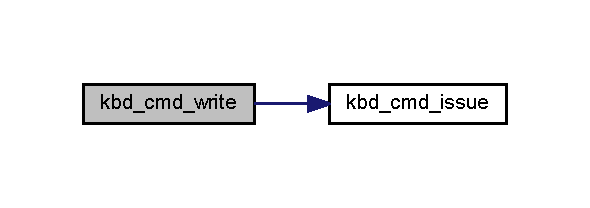
\includegraphics[width=283pt]{group__kbc_ga9a48bf91bd53208baa5627dd2a39e24d_cgraph}
\end{center}
\end{figure}
\hypertarget{group__kbc_ga8efa408da2468eaa11a0c515dfa8d79f}{}\label{group__kbc_ga8efa408da2468eaa11a0c515dfa8d79f} 
\index{kbc@{kbc}!kbd\+\_\+subscribe\+\_\+int@{kbd\+\_\+subscribe\+\_\+int}}
\index{kbd\+\_\+subscribe\+\_\+int@{kbd\+\_\+subscribe\+\_\+int}!kbc@{kbc}}
\subsubsection{\texorpdfstring{kbd\+\_\+subscribe\+\_\+int()}{kbd\_subscribe\_int()}}
{\footnotesize\ttfamily int kbd\+\_\+subscribe\+\_\+int (\begin{DoxyParamCaption}\item[{unsigned int $\ast$}]{kbd\+\_\+hook\+\_\+id }\end{DoxyParamCaption})}



subscribes a keyboard interruption 


\begin{DoxyParams}{Parameters}
{\em kbd\+\_\+hook\+\_\+id} & \\
\hline
\end{DoxyParams}
\begin{DoxyReturn}{Returns}
Return 0 upon success and non-\/zero otherwise 
\end{DoxyReturn}
\hypertarget{group__kbc_ga32ab97f6b806fa3a0524e62af55aeb0e}{}\label{group__kbc_ga32ab97f6b806fa3a0524e62af55aeb0e} 
\index{kbc@{kbc}!kbd\+\_\+unsubscribe\+\_\+int@{kbd\+\_\+unsubscribe\+\_\+int}}
\index{kbd\+\_\+unsubscribe\+\_\+int@{kbd\+\_\+unsubscribe\+\_\+int}!kbc@{kbc}}
\subsubsection{\texorpdfstring{kbd\+\_\+unsubscribe\+\_\+int()}{kbd\_unsubscribe\_int()}}
{\footnotesize\ttfamily int kbd\+\_\+unsubscribe\+\_\+int (\begin{DoxyParamCaption}\item[{unsigned int $\ast$}]{kbd\+\_\+hook\+\_\+id }\end{DoxyParamCaption})}



unsubscribes a keyboard interruption 


\begin{DoxyParams}{Parameters}
{\em kbd\+\_\+hook\+\_\+id} & \\
\hline
\end{DoxyParams}
\begin{DoxyReturn}{Returns}
Return 0 upon success and non-\/zero otherwise 
\end{DoxyReturn}

\hypertarget{group__lmlib}{}\section{lmlib}
\label{group__lmlib}\index{lmlib@{lmlib}}
\subsection*{Data Structures}
\begin{DoxyCompactItemize}
\item 
struct \hyperlink{structmmap__t}{mmap\+\_\+t}
\begin{DoxyCompactList}\small\item\em Memory Map Struct. \end{DoxyCompactList}\end{DoxyCompactItemize}
\subsection*{Functions}
\begin{DoxyCompactItemize}
\item 
void $\ast$ \hyperlink{group__lmlib_ga00a9c17c01e794a6bfc80fc5c6ab1ed1}{lm\+\_\+init} (void)
\begin{DoxyCompactList}\small\item\em Initializes the low memory area, the region up to the 1 M\+Byte physical address, by mapping it on the process\textquotesingle{} physical memory address. \end{DoxyCompactList}\item 
void $\ast$ \hyperlink{group__lmlib_gae45d971ce2ffcf4dc2677eba033a92cd}{lm\+\_\+alloc} (unsigned long size, \hyperlink{structmmap__t}{mmap\+\_\+t} $\ast$map)
\begin{DoxyCompactList}\small\item\em Allocates a memory block in low memory area with the specified size. \end{DoxyCompactList}\item 
void \hyperlink{group__lmlib_ga73e89d9c297b7390021fb545513579c6}{lm\+\_\+free} (\hyperlink{structmmap__t}{mmap\+\_\+t} $\ast$map)
\begin{DoxyCompactList}\small\item\em Frees a memory block in the low memory area, previously allocated using \hyperlink{group__lmlib_gae45d971ce2ffcf4dc2677eba033a92cd}{lm\+\_\+alloc()} \end{DoxyCompactList}\end{DoxyCompactItemize}
\subsection*{Variables}
\begin{DoxyCompactItemize}
\item 
phys\+\_\+bytes \hyperlink{group__lmlib_gab7a85fe0db943529016cf606e3a7167f}{phys}
\begin{DoxyCompactList}\small\item\em physical address \end{DoxyCompactList}\item 
void $\ast$ \hyperlink{group__lmlib_ga6a0ea2231d30f2b025e0c4b9f12dd6db}{virtual}
\begin{DoxyCompactList}\small\item\em virtual address \end{DoxyCompactList}\item 
unsigned long \hyperlink{group__lmlib_ga1e1268d164c38e4f8a4f4eb9058b0601}{size}
\begin{DoxyCompactList}\small\item\em size of memory region \end{DoxyCompactList}\end{DoxyCompactItemize}


\subsection{Detailed Description}
Functions related to low memory (first 1 MB of physical memory), required for B\+I\+OS 

\subsection{Function Documentation}
\hypertarget{group__lmlib_gae45d971ce2ffcf4dc2677eba033a92cd}{}\label{group__lmlib_gae45d971ce2ffcf4dc2677eba033a92cd} 
\index{lmlib@{lmlib}!lm\+\_\+alloc@{lm\+\_\+alloc}}
\index{lm\+\_\+alloc@{lm\+\_\+alloc}!lmlib@{lmlib}}
\subsubsection{\texorpdfstring{lm\+\_\+alloc()}{lm\_alloc()}}
{\footnotesize\ttfamily void$\ast$ lm\+\_\+alloc (\begin{DoxyParamCaption}\item[{unsigned long}]{size,  }\item[{\hyperlink{structmmap__t}{mmap\+\_\+t} $\ast$}]{map }\end{DoxyParamCaption})}



Allocates a memory block in low memory area with the specified size. 

Allocates a memory block in the region up to the 1 M\+Byte physical address with the input size. Initializes the input \hyperlink{structmmap__t}{mmap\+\_\+t} struct with the maping information, which can be read but must not be modified.


\begin{DoxyParams}{Parameters}
{\em size} & size of the memory block to allocate \\
\hline
{\em map} & pointer to \hyperlink{structmmap__t}{mmap\+\_\+t} data structure, which represents the memory map \\
\hline
\end{DoxyParams}
\begin{DoxyReturn}{Returns}
the virtual address of the memory block on success, N\+U\+LL otherwise 
\end{DoxyReturn}
\hypertarget{group__lmlib_ga73e89d9c297b7390021fb545513579c6}{}\label{group__lmlib_ga73e89d9c297b7390021fb545513579c6} 
\index{lmlib@{lmlib}!lm\+\_\+free@{lm\+\_\+free}}
\index{lm\+\_\+free@{lm\+\_\+free}!lmlib@{lmlib}}
\subsubsection{\texorpdfstring{lm\+\_\+free()}{lm\_free()}}
{\footnotesize\ttfamily void lm\+\_\+free (\begin{DoxyParamCaption}\item[{\hyperlink{structmmap__t}{mmap\+\_\+t} $\ast$}]{map }\end{DoxyParamCaption})}



Frees a memory block in the low memory area, previously allocated using \hyperlink{group__lmlib_gae45d971ce2ffcf4dc2677eba033a92cd}{lm\+\_\+alloc()} 

Frees a memory block in the region up to the 1 M\+Byte physical addess, previously allocated using \hyperlink{group__lmlib_gae45d971ce2ffcf4dc2677eba033a92cd}{lm\+\_\+alloc()}. Takes as input the address of the \hyperlink{structmmap__t}{mmap\+\_\+t} structure that was passed to \hyperlink{group__lmlib_gae45d971ce2ffcf4dc2677eba033a92cd}{lm\+\_\+alloc()}, and that must have not been modified since.


\begin{DoxyParams}{Parameters}
{\em map} & pointer to \hyperlink{structmmap__t}{mmap\+\_\+t} data structure of the block being freed \\
\hline
\end{DoxyParams}
\hypertarget{group__lmlib_ga00a9c17c01e794a6bfc80fc5c6ab1ed1}{}\label{group__lmlib_ga00a9c17c01e794a6bfc80fc5c6ab1ed1} 
\index{lmlib@{lmlib}!lm\+\_\+init@{lm\+\_\+init}}
\index{lm\+\_\+init@{lm\+\_\+init}!lmlib@{lmlib}}
\subsubsection{\texorpdfstring{lm\+\_\+init()}{lm\_init()}}
{\footnotesize\ttfamily void$\ast$ lm\+\_\+init (\begin{DoxyParamCaption}\item[{void}]{ }\end{DoxyParamCaption})}



Initializes the low memory area, the region up to the 1 M\+Byte physical address, by mapping it on the process\textquotesingle{} physical memory address. 

\begin{DoxyReturn}{Returns}
virtual address on which the first 1 MiB was mapped, N\+U\+LL upon failure 
\end{DoxyReturn}


\subsection{Variable Documentation}
\hypertarget{group__lmlib_gab7a85fe0db943529016cf606e3a7167f}{}\label{group__lmlib_gab7a85fe0db943529016cf606e3a7167f} 
\index{lmlib@{lmlib}!phys@{phys}}
\index{phys@{phys}!lmlib@{lmlib}}
\subsubsection{\texorpdfstring{phys}{phys}}
{\footnotesize\ttfamily phys\+\_\+bytes phys}



physical address 

\hypertarget{group__lmlib_ga1e1268d164c38e4f8a4f4eb9058b0601}{}\label{group__lmlib_ga1e1268d164c38e4f8a4f4eb9058b0601} 
\index{lmlib@{lmlib}!size@{size}}
\index{size@{size}!lmlib@{lmlib}}
\subsubsection{\texorpdfstring{size}{size}}
{\footnotesize\ttfamily unsigned long size}



size of memory region 

\hypertarget{group__lmlib_ga6a0ea2231d30f2b025e0c4b9f12dd6db}{}\label{group__lmlib_ga6a0ea2231d30f2b025e0c4b9f12dd6db} 
\index{lmlib@{lmlib}!virtual@{virtual}}
\index{virtual@{virtual}!lmlib@{lmlib}}
\subsubsection{\texorpdfstring{virtual}{virtual}}
{\footnotesize\ttfamily void$\ast$ virtual}



virtual address 


\hypertarget{group__mouse}{}\section{mouse}
\label{group__mouse}\index{mouse@{mouse}}
\subsection*{Data Structures}
\begin{DoxyCompactItemize}
\item 
struct \hyperlink{structmouse__packet__t}{mouse\+\_\+packet\+\_\+t}
\end{DoxyCompactItemize}
\subsection*{Functions}
\begin{DoxyCompactItemize}
\item 
int \hyperlink{group__mouse_gad607aaa8fd9833789fcd2b99c86dfc34}{mouse\+\_\+subscribe\+\_\+int} (unsigned int $\ast$mouse\+\_\+hook\+\_\+id)
\begin{DoxyCompactList}\small\item\em subscribes a mouse interruption \end{DoxyCompactList}\item 
int \hyperlink{group__mouse_gaa40354aab63adaf9ecddd01255efd918}{mouse\+\_\+unsubscribe\+\_\+int} (unsigned int $\ast$mouse\+\_\+hook\+\_\+id)
\begin{DoxyCompactList}\small\item\em unsubscribes a timer interruption \end{DoxyCompactList}\item 
int \hyperlink{group__mouse_ga42d943d35caacd5219cf4ef665b9bc42}{mouse\+\_\+cmd\+\_\+write} (unsigned long cmd)
\begin{DoxyCompactList}\small\item\em writes a command to kbd \end{DoxyCompactList}\item 
int \hyperlink{group__mouse_ga3a8a668ee784e6662fb1c2fd31e811b0}{mouse\+\_\+cmd\+\_\+read} (unsigned long $\ast$data)
\begin{DoxyCompactList}\small\item\em reads a command from mouse \end{DoxyCompactList}\item 
int \hyperlink{group__mouse_ga936c78f40a1d0b1acfd4f0368a9b8137}{mouse\+\_\+get\+\_\+packet} (unsigned long $\ast$next\+\_\+byte, unsigned char $\ast$packet)
\begin{DoxyCompactList}\small\item\em gets a packet from mouse \end{DoxyCompactList}\item 
void \hyperlink{group__mouse_gaf1a4587fac965330aca5079ae1313327}{mouse\+\_\+convert\+\_\+packet} (unsigned char $\ast$array\+\_\+packet, \hyperlink{structmouse__packet__t}{mouse\+\_\+packet\+\_\+t} $\ast$packet)
\begin{DoxyCompactList}\small\item\em convert a packet array to mouse packet that is more user friendly \end{DoxyCompactList}\end{DoxyCompactItemize}


\subsection{Detailed Description}
Functions to manipulate the mouse 

\subsection{Function Documentation}
\hypertarget{group__mouse_ga3a8a668ee784e6662fb1c2fd31e811b0}{}\label{group__mouse_ga3a8a668ee784e6662fb1c2fd31e811b0} 
\index{mouse@{mouse}!mouse\+\_\+cmd\+\_\+read@{mouse\+\_\+cmd\+\_\+read}}
\index{mouse\+\_\+cmd\+\_\+read@{mouse\+\_\+cmd\+\_\+read}!mouse@{mouse}}
\subsubsection{\texorpdfstring{mouse\+\_\+cmd\+\_\+read()}{mouse\_cmd\_read()}}
{\footnotesize\ttfamily int mouse\+\_\+cmd\+\_\+read (\begin{DoxyParamCaption}\item[{unsigned long $\ast$}]{data }\end{DoxyParamCaption})}



reads a command from mouse 


\begin{DoxyParams}{Parameters}
{\em data} & variable that stores the command \\
\hline
\end{DoxyParams}
\begin{DoxyReturn}{Returns}
Return 0 upon success and non-\/zero otherwise 
\end{DoxyReturn}
Here is the call graph for this function\+:
% FIG 0
\hypertarget{group__mouse_ga42d943d35caacd5219cf4ef665b9bc42}{}\label{group__mouse_ga42d943d35caacd5219cf4ef665b9bc42} 
\index{mouse@{mouse}!mouse\+\_\+cmd\+\_\+write@{mouse\+\_\+cmd\+\_\+write}}
\index{mouse\+\_\+cmd\+\_\+write@{mouse\+\_\+cmd\+\_\+write}!mouse@{mouse}}
\subsubsection{\texorpdfstring{mouse\+\_\+cmd\+\_\+write()}{mouse\_cmd\_write()}}
{\footnotesize\ttfamily int mouse\+\_\+cmd\+\_\+write (\begin{DoxyParamCaption}\item[{unsigned long}]{cmd }\end{DoxyParamCaption})}



writes a command to kbd 


\begin{DoxyParams}{Parameters}
{\em mouse\+\_\+hook\+\_\+id} & pointer to the hook of the mouse\\
\hline
{\em cmd} & command to be issued\\
\hline
\end{DoxyParams}
\begin{DoxyReturn}{Returns}
Return 0 upon success and non-\/zero otherwise 
\end{DoxyReturn}
Here is the call graph for this function\+:
% FIG 1
\hypertarget{group__mouse_gaf1a4587fac965330aca5079ae1313327}{}\label{group__mouse_gaf1a4587fac965330aca5079ae1313327} 
\index{mouse@{mouse}!mouse\+\_\+convert\+\_\+packet@{mouse\+\_\+convert\+\_\+packet}}
\index{mouse\+\_\+convert\+\_\+packet@{mouse\+\_\+convert\+\_\+packet}!mouse@{mouse}}
\subsubsection{\texorpdfstring{mouse\+\_\+convert\+\_\+packet()}{mouse\_convert\_packet()}}
{\footnotesize\ttfamily void mouse\+\_\+convert\+\_\+packet (\begin{DoxyParamCaption}\item[{unsigned char $\ast$}]{array\+\_\+packet,  }\item[{\hyperlink{structmouse__packet__t}{mouse\+\_\+packet\+\_\+t} $\ast$}]{packet }\end{DoxyParamCaption})}



convert a packet array to mouse packet that is more user friendly 


\begin{DoxyParams}{Parameters}
{\em array\+\_\+packet} & -\/$>$ array packet \\
\hline
{\em packet} & -\/$>$ variable that is going to store the mouse packet \\
\hline
\end{DoxyParams}
Here is the call graph for this function\+:
% FIG 2
\hypertarget{group__mouse_ga936c78f40a1d0b1acfd4f0368a9b8137}{}\label{group__mouse_ga936c78f40a1d0b1acfd4f0368a9b8137} 
\index{mouse@{mouse}!mouse\+\_\+get\+\_\+packet@{mouse\+\_\+get\+\_\+packet}}
\index{mouse\+\_\+get\+\_\+packet@{mouse\+\_\+get\+\_\+packet}!mouse@{mouse}}
\subsubsection{\texorpdfstring{mouse\+\_\+get\+\_\+packet()}{mouse\_get\_packet()}}
{\footnotesize\ttfamily int mouse\+\_\+get\+\_\+packet (\begin{DoxyParamCaption}\item[{unsigned long $\ast$}]{next\+\_\+byte,  }\item[{unsigned char $\ast$}]{packet }\end{DoxyParamCaption})}



gets a packet from mouse 


\begin{DoxyParams}{Parameters}
{\em next\+\_\+byte} & next\+\_\+byte of the packet to be read \\
\hline
{\em packet} & variable that is going to store the packet \\
\hline
\end{DoxyParams}
\begin{DoxyReturn}{Returns}
Return 0 upon success and non-\/zero otherwise 
\end{DoxyReturn}
Here is the call graph for this function\+:
% FIG 3
\hypertarget{group__mouse_gad607aaa8fd9833789fcd2b99c86dfc34}{}\label{group__mouse_gad607aaa8fd9833789fcd2b99c86dfc34} 
\index{mouse@{mouse}!mouse\+\_\+subscribe\+\_\+int@{mouse\+\_\+subscribe\+\_\+int}}
\index{mouse\+\_\+subscribe\+\_\+int@{mouse\+\_\+subscribe\+\_\+int}!mouse@{mouse}}
\subsubsection{\texorpdfstring{mouse\+\_\+subscribe\+\_\+int()}{mouse\_subscribe\_int()}}
{\footnotesize\ttfamily int mouse\+\_\+subscribe\+\_\+int (\begin{DoxyParamCaption}\item[{unsigned int $\ast$}]{mouse\+\_\+hook\+\_\+id }\end{DoxyParamCaption})}



subscribes a mouse interruption 

\begin{DoxyReturn}{Returns}
Return 0 upon success and non-\/zero otherwise 
\end{DoxyReturn}
\hypertarget{group__mouse_gaa40354aab63adaf9ecddd01255efd918}{}\label{group__mouse_gaa40354aab63adaf9ecddd01255efd918} 
\index{mouse@{mouse}!mouse\+\_\+unsubscribe\+\_\+int@{mouse\+\_\+unsubscribe\+\_\+int}}
\index{mouse\+\_\+unsubscribe\+\_\+int@{mouse\+\_\+unsubscribe\+\_\+int}!mouse@{mouse}}
\subsubsection{\texorpdfstring{mouse\+\_\+unsubscribe\+\_\+int()}{mouse\_unsubscribe\_int()}}
{\footnotesize\ttfamily int mouse\+\_\+unsubscribe\+\_\+int (\begin{DoxyParamCaption}\item[{unsigned int $\ast$}]{mouse\+\_\+hook\+\_\+id }\end{DoxyParamCaption})}



unsubscribes a timer interruption 


\begin{DoxyParams}{Parameters}
{\em mouse\+\_\+hook\+\_\+id} & pointer to the hook of the mouse\\
\hline
\end{DoxyParams}
\begin{DoxyReturn}{Returns}
Return 0 upon success and non-\/zero otherwise 
\end{DoxyReturn}

\hypertarget{group___program_logic}{}\section{Program\+Logic}
\label{group___program_logic}\index{Program\+Logic@{Program\+Logic}}
\subsection*{Functions}
\begin{DoxyCompactItemize}
\item 
int \hyperlink{group___program_logic_ga2838b9e6247aa4515f76cfeccf8e1cd8}{create\+Board} (char \hyperlink{checkers_8c_a12f50bd537a3a737da9d47710c308ae3}{board}\mbox{[}8\mbox{]}\mbox{[}8\mbox{]})
\begin{DoxyCompactList}\small\item\em Creates the board with initial positions. \end{DoxyCompactList}\item 
int \hyperlink{group___program_logic_ga02801d684d1f985fcaff098e12a0bf59}{move\+Disc} (char \hyperlink{checkers_8c_a12f50bd537a3a737da9d47710c308ae3}{board}\mbox{[}8\mbox{]}\mbox{[}8\mbox{]}, char player, int xi, int yi, int xf, int yf)
\begin{DoxyCompactList}\small\item\em Moves disc in the given position(xi,yi) to final position also given(xf,yf). \end{DoxyCompactList}\item 
int \hyperlink{group___program_logic_gaed1b217c7e40a6fb27a0e6a719594aba}{is\+Position\+Initial\+Valid} (char \hyperlink{checkers_8c_a12f50bd537a3a737da9d47710c308ae3}{board}\mbox{[}8\mbox{]}\mbox{[}8\mbox{]}, char player, int xi, int yi)
\begin{DoxyCompactList}\small\item\em Verifies if given initial position(xi,yi) is valid or not. \end{DoxyCompactList}\item 
int \hyperlink{group___program_logic_ga0862e9966f69666bb39dbf1c58863c3b}{verify\+Capture\+Move} (char \hyperlink{checkers_8c_a12f50bd537a3a737da9d47710c308ae3}{board}\mbox{[}8\mbox{]}\mbox{[}8\mbox{]}, char player, int xi, int yi)
\begin{DoxyCompactList}\small\item\em Verifies if given initial position(xi,yi) can do a capture move or not. \end{DoxyCompactList}\item 
void \hyperlink{group___program_logic_ga484dd8982591f724c6ff6749bba6869a}{move\+To\+Final} (char \hyperlink{checkers_8c_a12f50bd537a3a737da9d47710c308ae3}{board}\mbox{[}8\mbox{]}\mbox{[}8\mbox{]}, int xi, int yi, int xf, int yf)
\begin{DoxyCompactList}\small\item\em Moves disc in the given position(xi,yi) to final position also given(xf,yf). \end{DoxyCompactList}\item 
void \hyperlink{group___program_logic_ga5de7cebab5418f009cebb5dc73e50cd2}{make\+Capture\+Move} (char \hyperlink{checkers_8c_a12f50bd537a3a737da9d47710c308ae3}{board}\mbox{[}8\mbox{]}\mbox{[}8\mbox{]}, int xi, int yi, int xf, int yf)
\begin{DoxyCompactList}\small\item\em Moves disc in the given position(xi,yi) to final position also given(xf,yf), making a capture move. \end{DoxyCompactList}\item 
int \hyperlink{group___program_logic_gacfd2089a907444dab0ccd2d95f321b8b}{is\+End\+Game} (char \hyperlink{checkers_8c_a12f50bd537a3a737da9d47710c308ae3}{board}\mbox{[}8\mbox{]}\mbox{[}8\mbox{]})
\begin{DoxyCompactList}\small\item\em Verifies if it is the end of the game. \end{DoxyCompactList}\item 
int $\ast$ \hyperlink{group___program_logic_ga8d87858478876b33304e38cea751951b}{moves\+I\+Can\+Do} (char \hyperlink{checkers_8c_a12f50bd537a3a737da9d47710c308ae3}{board}\mbox{[}8\mbox{]}\mbox{[}8\mbox{]}, char player, int xi, int yi)
\begin{DoxyCompactList}\small\item\em Gives the moves that a disc can make. \end{DoxyCompactList}\end{DoxyCompactItemize}


\subsection{Detailed Description}
Functions for the logical part of the game 

\subsection{Function Documentation}
\hypertarget{group___program_logic_ga2838b9e6247aa4515f76cfeccf8e1cd8}{}\label{group___program_logic_ga2838b9e6247aa4515f76cfeccf8e1cd8} 
\index{Program\+Logic@{Program\+Logic}!create\+Board@{create\+Board}}
\index{create\+Board@{create\+Board}!Program\+Logic@{Program\+Logic}}
\subsubsection{\texorpdfstring{create\+Board()}{createBoard()}}
{\footnotesize\ttfamily int create\+Board (\begin{DoxyParamCaption}\item[{char}]{board\mbox{[}8\mbox{]}\mbox{[}8\mbox{]} }\end{DoxyParamCaption})}



Creates the board with initial positions. 

0 -\/ empty position;

1 -\/ black discs (player 1);

2 -\/ white discs (player 2).


\begin{DoxyParams}{Parameters}
{\em board\mbox{[}8\mbox{]}\mbox{[}8\mbox{]}} & array of arrays with current game status. \\
\hline
\end{DoxyParams}
\begin{DoxyReturn}{Returns}
returns 0 if successful. 
\end{DoxyReturn}
\hypertarget{group___program_logic_gacfd2089a907444dab0ccd2d95f321b8b}{}\label{group___program_logic_gacfd2089a907444dab0ccd2d95f321b8b} 
\index{Program\+Logic@{Program\+Logic}!is\+End\+Game@{is\+End\+Game}}
\index{is\+End\+Game@{is\+End\+Game}!Program\+Logic@{Program\+Logic}}
\subsubsection{\texorpdfstring{is\+End\+Game()}{isEndGame()}}
{\footnotesize\ttfamily int is\+End\+Game (\begin{DoxyParamCaption}\item[{char}]{board\mbox{[}8\mbox{]}\mbox{[}8\mbox{]} }\end{DoxyParamCaption})}



Verifies if it is the end of the game. 


\begin{DoxyParams}{Parameters}
{\em board\mbox{[}8\mbox{]}\mbox{[}8\mbox{]}} & -\/$>$ array of arrays with current game status. \\
\hline
\end{DoxyParams}
\begin{DoxyReturn}{Returns}
0 if it\textquotesingle{}s not the end of the game; 

1 if it\textquotesingle{}s the end of the game. 
\end{DoxyReturn}
\hypertarget{group___program_logic_gaed1b217c7e40a6fb27a0e6a719594aba}{}\label{group___program_logic_gaed1b217c7e40a6fb27a0e6a719594aba} 
\index{Program\+Logic@{Program\+Logic}!is\+Position\+Initial\+Valid@{is\+Position\+Initial\+Valid}}
\index{is\+Position\+Initial\+Valid@{is\+Position\+Initial\+Valid}!Program\+Logic@{Program\+Logic}}
\subsubsection{\texorpdfstring{is\+Position\+Initial\+Valid()}{isPositionInitialValid()}}
{\footnotesize\ttfamily int is\+Position\+Initial\+Valid (\begin{DoxyParamCaption}\item[{char}]{board\mbox{[}8\mbox{]}\mbox{[}8\mbox{]},  }\item[{char}]{player,  }\item[{int}]{xi,  }\item[{int}]{yi }\end{DoxyParamCaption})}



Verifies if given initial position(xi,yi) is valid or not. 


\begin{DoxyParams}{Parameters}
{\em board\mbox{[}8\mbox{]}\mbox{[}8\mbox{]}} & array of arrays with current game status; \\
\hline
{\em player} & the player who is going to play (1-\/player with black discs; 2-\/player with white discs); \\
\hline
{\em xi} & initial position x component; \\
\hline
{\em yi} & initial position y component. \\
\hline
\end{DoxyParams}
\begin{DoxyReturn}{Returns}
0 if valid position; 

1 if invalid position. 
\end{DoxyReturn}
Here is the call graph for this function\+:\nopagebreak
\begin{figure}[H]
\begin{center}
\leavevmode
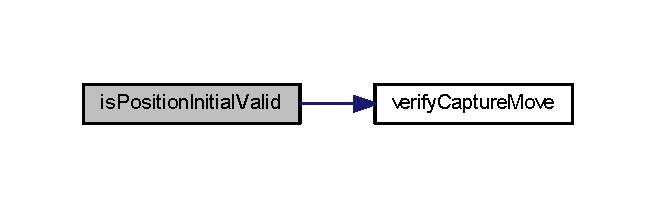
\includegraphics[width=315pt]{group___program_logic_gaed1b217c7e40a6fb27a0e6a719594aba_cgraph}
\end{center}
\end{figure}
\hypertarget{group___program_logic_ga5de7cebab5418f009cebb5dc73e50cd2}{}\label{group___program_logic_ga5de7cebab5418f009cebb5dc73e50cd2} 
\index{Program\+Logic@{Program\+Logic}!make\+Capture\+Move@{make\+Capture\+Move}}
\index{make\+Capture\+Move@{make\+Capture\+Move}!Program\+Logic@{Program\+Logic}}
\subsubsection{\texorpdfstring{make\+Capture\+Move()}{makeCaptureMove()}}
{\footnotesize\ttfamily void make\+Capture\+Move (\begin{DoxyParamCaption}\item[{char}]{board\mbox{[}8\mbox{]}\mbox{[}8\mbox{]},  }\item[{int}]{xi,  }\item[{int}]{yi,  }\item[{int}]{xf,  }\item[{int}]{yf }\end{DoxyParamCaption})}



Moves disc in the given position(xi,yi) to final position also given(xf,yf), making a capture move. 


\begin{DoxyParams}{Parameters}
{\em board\mbox{[}8\mbox{]}\mbox{[}8\mbox{]}} & -\/$>$ array of arrays with current game status; \\
\hline
{\em xi} & initial position x component; \\
\hline
{\em yi} & initial position y component; \\
\hline
{\em xf} & final position x component; \\
\hline
{\em yf} & final position y component. \\
\hline
\end{DoxyParams}
\hypertarget{group___program_logic_ga02801d684d1f985fcaff098e12a0bf59}{}\label{group___program_logic_ga02801d684d1f985fcaff098e12a0bf59} 
\index{Program\+Logic@{Program\+Logic}!move\+Disc@{move\+Disc}}
\index{move\+Disc@{move\+Disc}!Program\+Logic@{Program\+Logic}}
\subsubsection{\texorpdfstring{move\+Disc()}{moveDisc()}}
{\footnotesize\ttfamily int move\+Disc (\begin{DoxyParamCaption}\item[{char}]{board\mbox{[}8\mbox{]}\mbox{[}8\mbox{]},  }\item[{char}]{player,  }\item[{int}]{xi,  }\item[{int}]{yi,  }\item[{int}]{xf,  }\item[{int}]{yf }\end{DoxyParamCaption})}



Moves disc in the given position(xi,yi) to final position also given(xf,yf). 


\begin{DoxyParams}{Parameters}
{\em board\mbox{[}8\mbox{]}\mbox{[}8\mbox{]}} & array of arrays with current game status; \\
\hline
{\em player} & the player who is going to play (1-\/player with black discs; 2-\/player with white discs); \\
\hline
{\em xi} & initial position x component; \\
\hline
{\em yi} & initial position y component; \\
\hline
{\em xf} & final position x component; \\
\hline
{\em yf} & final position y component. \\
\hline
\end{DoxyParams}
\begin{DoxyReturn}{Returns}
0 if invalid play; 

1 if valid play -\/ move disc to right side; 

2 if valid play -\/ move disc to left side; 

3 if valid play -\/ capture disc to right side; 

4 if valid play -\/ capture disc to left side; 

5 if invalid play -\/ has to capture a disc; 

6 if invalid play -\/ has to capture a disc with another initial position. 
\end{DoxyReturn}
Here is the call graph for this function\+:\nopagebreak
\begin{figure}[H]
\begin{center}
\leavevmode
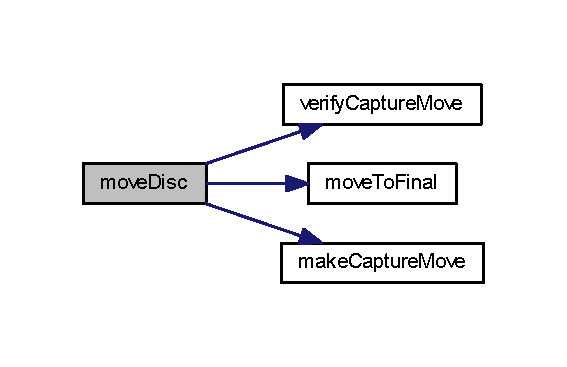
\includegraphics[width=272pt]{group___program_logic_ga02801d684d1f985fcaff098e12a0bf59_cgraph}
\end{center}
\end{figure}
\hypertarget{group___program_logic_ga8d87858478876b33304e38cea751951b}{}\label{group___program_logic_ga8d87858478876b33304e38cea751951b} 
\index{Program\+Logic@{Program\+Logic}!moves\+I\+Can\+Do@{moves\+I\+Can\+Do}}
\index{moves\+I\+Can\+Do@{moves\+I\+Can\+Do}!Program\+Logic@{Program\+Logic}}
\subsubsection{\texorpdfstring{moves\+I\+Can\+Do()}{movesICanDo()}}
{\footnotesize\ttfamily int$\ast$ moves\+I\+Can\+Do (\begin{DoxyParamCaption}\item[{char}]{board\mbox{[}8\mbox{]}\mbox{[}8\mbox{]},  }\item[{char}]{player,  }\item[{int}]{xi,  }\item[{int}]{yi }\end{DoxyParamCaption})}



Gives the moves that a disc can make. 


\begin{DoxyParams}{Parameters}
{\em board\mbox{[}8\mbox{]}\mbox{[}8\mbox{]}} & array of arrays with current game status; \\
\hline
{\em player} & the player who is going to play (1-\/player with black discs; 2-\/player with white discs); \\
\hline
\end{DoxyParams}
\begin{DoxyReturn}{Returns}
returns an array of integers(r\mbox{[}5\mbox{]}) with the positions we can move to\+: 

r\mbox{[}0\mbox{]} number of positions we can use(0,1 or 2); 

r\mbox{[}1\mbox{]} and r\mbox{[}2\mbox{]} x and y, respectively, of a position we can move to (used if r\mbox{[}0\mbox{]}==1 or r\mbox{[}0\mbox{]}==2); 

r\mbox{[}3\mbox{]} and r\mbox{[}4\mbox{]} x and y, respectively, of a position we can move to (used if r\mbox{[}0\mbox{]}==2). 
\end{DoxyReturn}
Here is the call graph for this function\+:\nopagebreak
\begin{figure}[H]
\begin{center}
\leavevmode
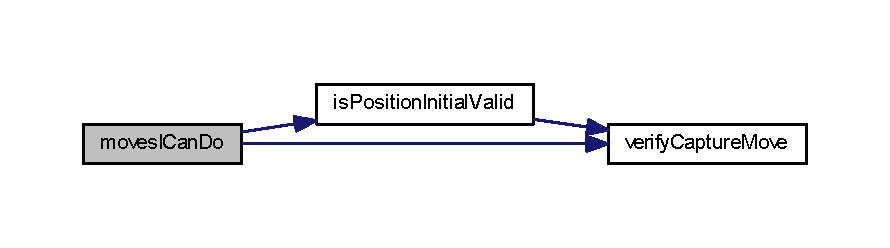
\includegraphics[width=350pt]{group___program_logic_ga8d87858478876b33304e38cea751951b_cgraph}
\end{center}
\end{figure}
\hypertarget{group___program_logic_ga484dd8982591f724c6ff6749bba6869a}{}\label{group___program_logic_ga484dd8982591f724c6ff6749bba6869a} 
\index{Program\+Logic@{Program\+Logic}!move\+To\+Final@{move\+To\+Final}}
\index{move\+To\+Final@{move\+To\+Final}!Program\+Logic@{Program\+Logic}}
\subsubsection{\texorpdfstring{move\+To\+Final()}{moveToFinal()}}
{\footnotesize\ttfamily void move\+To\+Final (\begin{DoxyParamCaption}\item[{char}]{board\mbox{[}8\mbox{]}\mbox{[}8\mbox{]},  }\item[{int}]{xi,  }\item[{int}]{yi,  }\item[{int}]{xf,  }\item[{int}]{yf }\end{DoxyParamCaption})}



Moves disc in the given position(xi,yi) to final position also given(xf,yf). 


\begin{DoxyParams}{Parameters}
{\em board\mbox{[}8\mbox{]}\mbox{[}8\mbox{]}} & array of arrays with current game status; \\
\hline
{\em xi} & initial position x component; \\
\hline
{\em yi} & initial position y component; \\
\hline
{\em xf} & final position x component; \\
\hline
{\em yf} & final position y component. \\
\hline
\end{DoxyParams}
\hypertarget{group___program_logic_ga0862e9966f69666bb39dbf1c58863c3b}{}\label{group___program_logic_ga0862e9966f69666bb39dbf1c58863c3b} 
\index{Program\+Logic@{Program\+Logic}!verify\+Capture\+Move@{verify\+Capture\+Move}}
\index{verify\+Capture\+Move@{verify\+Capture\+Move}!Program\+Logic@{Program\+Logic}}
\subsubsection{\texorpdfstring{verify\+Capture\+Move()}{verifyCaptureMove()}}
{\footnotesize\ttfamily int verify\+Capture\+Move (\begin{DoxyParamCaption}\item[{char}]{board\mbox{[}8\mbox{]}\mbox{[}8\mbox{]},  }\item[{char}]{player,  }\item[{int}]{xi,  }\item[{int}]{yi }\end{DoxyParamCaption})}



Verifies if given initial position(xi,yi) can do a capture move or not. 


\begin{DoxyParams}{Parameters}
{\em board\mbox{[}8\mbox{]}\mbox{[}8\mbox{]}} & array of arrays with current game status; \\
\hline
{\em player} & the player who is going to play (1-\/player with black discs; 2-\/player with white discs); \\
\hline
{\em xi} & initial position x component; \\
\hline
{\em yi} & initial position y component. \\
\hline
\end{DoxyParams}
\begin{DoxyReturn}{Returns}
0 if cant make any cature moves; 

1 if can do a capture move to right side; 

2 if can do a capture move to left side; 

3 if can do a capture move to both sides. 
\end{DoxyReturn}

\hypertarget{group__proj}{}\section{proj}
\label{group__proj}\index{proj@{proj}}
\subsection*{Macros}
\begin{DoxyCompactItemize}
\item 
\#define \hyperlink{group__proj_ga698fc99ce97e8051ede3e8e9c9baaaf1}{P\+O\+R\+T\+\_\+\+A\+D\+DR}~\hyperlink{group__ser__port_ga98199cd85fbe47b9a741b07762260422}{S\+E\+R\+\_\+\+C\+O\+M1\+\_\+\+A\+D\+DR}
\item 
\#define \hyperlink{group__proj_ga108355009766d90bac37c294fad39ca5}{P\+O\+R\+T\+\_\+\+B\+I\+TS}~8
\item 
\#define \hyperlink{group__proj_ga31b06d45be51d1c232d4cb34be4d385b}{P\+O\+R\+T\+\_\+\+S\+T\+OP}~2
\item 
\#define \hyperlink{group__proj_gaf868e5bf4fd27a5f53de530ce879dee4}{P\+O\+R\+T\+\_\+\+P\+A\+R\+I\+TY}~0
\item 
\#define \hyperlink{group__proj_gaa892a49ac9cab99bd99907f48a535b72}{P\+O\+R\+T\+\_\+\+R\+A\+TE}~9600
\end{DoxyCompactItemize}
\subsection*{Functions}
\begin{DoxyCompactItemize}
\item 
int \hyperlink{group__proj_ga3c04138a5bfe5d72780bb7e82a18e627}{main} (int argc, char $\ast$$\ast$argv)
\begin{DoxyCompactList}\small\item\em Main Function. \end{DoxyCompactList}\item 
static void \hyperlink{group__proj_ga7721a8566abc323f59672fdde30d3e20}{print\+\_\+usage} (char $\ast$$\ast$argv)
\begin{DoxyCompactList}\small\item\em print\+\_\+usage \end{DoxyCompactList}\item 
static int \hyperlink{group__proj_ga97b25d50dc55b5c8c2315fd010bc2957}{proc\+\_\+args} (int argc, char $\ast$$\ast$argv)
\begin{DoxyCompactList}\small\item\em print\+\_\+args \end{DoxyCompactList}\item 
static void \hyperlink{group__proj_ga3310cf47c29dd0f685c58e04fac7be4a}{ret\+\_\+path\+\_\+images} (char $\ast$arg, char $\ast$path\+\_\+images)
\begin{DoxyCompactList}\small\item\em ret\+\_\+path\+\_\+images \end{DoxyCompactList}\item 
int \hyperlink{group__proj_gac4a55a52afabd10db600de603282ff99}{connect\+\_\+serial} (char player, char $\ast$arg0)
\begin{DoxyCompactList}\small\item\em establishes a connection in the serial port \end{DoxyCompactList}\end{DoxyCompactItemize}


\subsection{Detailed Description}
Main function and serial port connection function 

\subsection{Macro Definition Documentation}
\hypertarget{group__proj_ga698fc99ce97e8051ede3e8e9c9baaaf1}{}\label{group__proj_ga698fc99ce97e8051ede3e8e9c9baaaf1} 
\index{proj@{proj}!P\+O\+R\+T\+\_\+\+A\+D\+DR@{P\+O\+R\+T\+\_\+\+A\+D\+DR}}
\index{P\+O\+R\+T\+\_\+\+A\+D\+DR@{P\+O\+R\+T\+\_\+\+A\+D\+DR}!proj@{proj}}
\subsubsection{\texorpdfstring{P\+O\+R\+T\+\_\+\+A\+D\+DR}{PORT\_ADDR}}
{\footnotesize\ttfamily \#define P\+O\+R\+T\+\_\+\+A\+D\+DR~\hyperlink{group__ser__port_ga98199cd85fbe47b9a741b07762260422}{S\+E\+R\+\_\+\+C\+O\+M1\+\_\+\+A\+D\+DR}}

\hypertarget{group__proj_ga108355009766d90bac37c294fad39ca5}{}\label{group__proj_ga108355009766d90bac37c294fad39ca5} 
\index{proj@{proj}!P\+O\+R\+T\+\_\+\+B\+I\+TS@{P\+O\+R\+T\+\_\+\+B\+I\+TS}}
\index{P\+O\+R\+T\+\_\+\+B\+I\+TS@{P\+O\+R\+T\+\_\+\+B\+I\+TS}!proj@{proj}}
\subsubsection{\texorpdfstring{P\+O\+R\+T\+\_\+\+B\+I\+TS}{PORT\_BITS}}
{\footnotesize\ttfamily \#define P\+O\+R\+T\+\_\+\+B\+I\+TS~8}

\hypertarget{group__proj_gaf868e5bf4fd27a5f53de530ce879dee4}{}\label{group__proj_gaf868e5bf4fd27a5f53de530ce879dee4} 
\index{proj@{proj}!P\+O\+R\+T\+\_\+\+P\+A\+R\+I\+TY@{P\+O\+R\+T\+\_\+\+P\+A\+R\+I\+TY}}
\index{P\+O\+R\+T\+\_\+\+P\+A\+R\+I\+TY@{P\+O\+R\+T\+\_\+\+P\+A\+R\+I\+TY}!proj@{proj}}
\subsubsection{\texorpdfstring{P\+O\+R\+T\+\_\+\+P\+A\+R\+I\+TY}{PORT\_PARITY}}
{\footnotesize\ttfamily \#define P\+O\+R\+T\+\_\+\+P\+A\+R\+I\+TY~0}

\hypertarget{group__proj_gaa892a49ac9cab99bd99907f48a535b72}{}\label{group__proj_gaa892a49ac9cab99bd99907f48a535b72} 
\index{proj@{proj}!P\+O\+R\+T\+\_\+\+R\+A\+TE@{P\+O\+R\+T\+\_\+\+R\+A\+TE}}
\index{P\+O\+R\+T\+\_\+\+R\+A\+TE@{P\+O\+R\+T\+\_\+\+R\+A\+TE}!proj@{proj}}
\subsubsection{\texorpdfstring{P\+O\+R\+T\+\_\+\+R\+A\+TE}{PORT\_RATE}}
{\footnotesize\ttfamily \#define P\+O\+R\+T\+\_\+\+R\+A\+TE~9600}

\hypertarget{group__proj_ga31b06d45be51d1c232d4cb34be4d385b}{}\label{group__proj_ga31b06d45be51d1c232d4cb34be4d385b} 
\index{proj@{proj}!P\+O\+R\+T\+\_\+\+S\+T\+OP@{P\+O\+R\+T\+\_\+\+S\+T\+OP}}
\index{P\+O\+R\+T\+\_\+\+S\+T\+OP@{P\+O\+R\+T\+\_\+\+S\+T\+OP}!proj@{proj}}
\subsubsection{\texorpdfstring{P\+O\+R\+T\+\_\+\+S\+T\+OP}{PORT\_STOP}}
{\footnotesize\ttfamily \#define P\+O\+R\+T\+\_\+\+S\+T\+OP~2}



\subsection{Function Documentation}
\hypertarget{group__proj_gac4a55a52afabd10db600de603282ff99}{}\label{group__proj_gac4a55a52afabd10db600de603282ff99} 
\index{proj@{proj}!connect\+\_\+serial@{connect\+\_\+serial}}
\index{connect\+\_\+serial@{connect\+\_\+serial}!proj@{proj}}
\subsubsection{\texorpdfstring{connect\+\_\+serial()}{connect\_serial()}}
{\footnotesize\ttfamily int connect\+\_\+serial (\begin{DoxyParamCaption}\item[{char}]{player,  }\item[{char $\ast$}]{arg0 }\end{DoxyParamCaption})}



establishes a connection in the serial port 


\begin{DoxyParams}{Parameters}
{\em player} & player that is establishing the connection \\
\hline
{\em arg0} & parameter that will later be used to find the images path \\
\hline
\end{DoxyParams}
\begin{DoxyReturn}{Returns}
0 in case of success, 1 otherwise 
\end{DoxyReturn}
Here is the call graph for this function\+:
% FIG 0
\hypertarget{group__proj_ga3c04138a5bfe5d72780bb7e82a18e627}{}\label{group__proj_ga3c04138a5bfe5d72780bb7e82a18e627} 
\index{proj@{proj}!main@{main}}
\index{main@{main}!proj@{proj}}
\subsubsection{\texorpdfstring{main()}{main()}}
{\footnotesize\ttfamily int main (\begin{DoxyParamCaption}\item[{int}]{argc,  }\item[{char $\ast$$\ast$}]{argv }\end{DoxyParamCaption})}



Main Function. 

Here is the call graph for this function\+:
% FIG 1
\hypertarget{group__proj_ga7721a8566abc323f59672fdde30d3e20}{}\label{group__proj_ga7721a8566abc323f59672fdde30d3e20} 
\index{proj@{proj}!print\+\_\+usage@{print\+\_\+usage}}
\index{print\+\_\+usage@{print\+\_\+usage}!proj@{proj}}
\subsubsection{\texorpdfstring{print\+\_\+usage()}{print\_usage()}}
{\footnotesize\ttfamily static void print\+\_\+usage (\begin{DoxyParamCaption}\item[{char $\ast$$\ast$}]{argv }\end{DoxyParamCaption})\hspace{0.3cm}{\ttfamily [static]}}



print\+\_\+usage 

\hypertarget{group__proj_ga97b25d50dc55b5c8c2315fd010bc2957}{}\label{group__proj_ga97b25d50dc55b5c8c2315fd010bc2957} 
\index{proj@{proj}!proc\+\_\+args@{proc\+\_\+args}}
\index{proc\+\_\+args@{proc\+\_\+args}!proj@{proj}}
\subsubsection{\texorpdfstring{proc\+\_\+args()}{proc\_args()}}
{\footnotesize\ttfamily static int proc\+\_\+args (\begin{DoxyParamCaption}\item[{int}]{argc,  }\item[{char $\ast$$\ast$}]{argv }\end{DoxyParamCaption})\hspace{0.3cm}{\ttfamily [static]}}



print\+\_\+args 

\hypertarget{group__proj_ga3310cf47c29dd0f685c58e04fac7be4a}{}\label{group__proj_ga3310cf47c29dd0f685c58e04fac7be4a} 
\index{proj@{proj}!ret\+\_\+path\+\_\+images@{ret\+\_\+path\+\_\+images}}
\index{ret\+\_\+path\+\_\+images@{ret\+\_\+path\+\_\+images}!proj@{proj}}
\subsubsection{\texorpdfstring{ret\+\_\+path\+\_\+images()}{ret\_path\_images()}}
{\footnotesize\ttfamily static void ret\+\_\+path\+\_\+images (\begin{DoxyParamCaption}\item[{char $\ast$}]{arg,  }\item[{char $\ast$}]{path\+\_\+images }\end{DoxyParamCaption})\hspace{0.3cm}{\ttfamily [static]}}



ret\+\_\+path\+\_\+images 


\hypertarget{group__publicity}{}\section{publicity}
\label{group__publicity}\index{publicity@{publicity}}
\subsection*{Functions}
\begin{DoxyCompactItemize}
\item 
int \hyperlink{group__publicity_ga7a04ef3aec214c81663352a9f4f35a65}{show\+\_\+ad} (char $\ast$path\+\_\+images)
\begin{DoxyCompactList}\small\item\em shows an ad. If today is a day of the week shows a certain ad, if it\textquotesingle{}s weekend shows another one \end{DoxyCompactList}\item 
int \hyperlink{group__publicity_ga7bad5577543cdab533e3bc88669cd691}{Isweekend} (\hyperlink{structdate__t}{date\+\_\+t} date)
\begin{DoxyCompactList}\small\item\em Determines if date is a weekend or not. \end{DoxyCompactList}\item 
int \hyperlink{group__publicity_ga2ff0d1265d48a43111f38f357dd1f874}{Isleap} (int year)
\begin{DoxyCompactList}\small\item\em Determines is year is leap or not. \end{DoxyCompactList}\end{DoxyCompactItemize}


\subsection{Detailed Description}
Functions for publicity 

\subsection{Function Documentation}
\hypertarget{group__publicity_ga2ff0d1265d48a43111f38f357dd1f874}{}\label{group__publicity_ga2ff0d1265d48a43111f38f357dd1f874} 
\index{publicity@{publicity}!Isleap@{Isleap}}
\index{Isleap@{Isleap}!publicity@{publicity}}
\subsubsection{\texorpdfstring{Isleap()}{Isleap()}}
{\footnotesize\ttfamily int Isleap (\begin{DoxyParamCaption}\item[{int}]{year }\end{DoxyParamCaption})}



Determines is year is leap or not. 


\begin{DoxyParams}{Parameters}
{\em year} & \\
\hline
\end{DoxyParams}
\begin{DoxyReturn}{Returns}
1 if a year is leap, 0 otherwise 
\end{DoxyReturn}
\hypertarget{group__publicity_ga7bad5577543cdab533e3bc88669cd691}{}\label{group__publicity_ga7bad5577543cdab533e3bc88669cd691} 
\index{publicity@{publicity}!Isweekend@{Isweekend}}
\index{Isweekend@{Isweekend}!publicity@{publicity}}
\subsubsection{\texorpdfstring{Isweekend()}{Isweekend()}}
{\footnotesize\ttfamily int Isweekend (\begin{DoxyParamCaption}\item[{\hyperlink{structdate__t}{date\+\_\+t}}]{date }\end{DoxyParamCaption})}



Determines if date is a weekend or not. 


\begin{DoxyParams}{Parameters}
{\em date} & \\
\hline
\end{DoxyParams}
\begin{DoxyReturn}{Returns}
1 if a date is weekend, 0 otherwise 
\end{DoxyReturn}
Here is the call graph for this function\+:\nopagebreak
\begin{figure}[H]
\begin{center}
\leavevmode
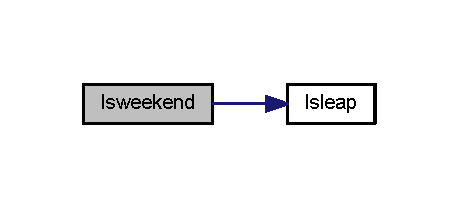
\includegraphics[width=220pt]{group__publicity_ga7bad5577543cdab533e3bc88669cd691_cgraph}
\end{center}
\end{figure}
\hypertarget{group__publicity_ga7a04ef3aec214c81663352a9f4f35a65}{}\label{group__publicity_ga7a04ef3aec214c81663352a9f4f35a65} 
\index{publicity@{publicity}!show\+\_\+ad@{show\+\_\+ad}}
\index{show\+\_\+ad@{show\+\_\+ad}!publicity@{publicity}}
\subsubsection{\texorpdfstring{show\+\_\+ad()}{show\_ad()}}
{\footnotesize\ttfamily int show\+\_\+ad (\begin{DoxyParamCaption}\item[{char $\ast$}]{path\+\_\+images }\end{DoxyParamCaption})}



shows an ad. If today is a day of the week shows a certain ad, if it\textquotesingle{}s weekend shows another one 


\begin{DoxyParams}{Parameters}
{\em path\+\_\+images} & path of the images directory \\
\hline
\end{DoxyParams}
\begin{DoxyReturn}{Returns}
1 in case of success, 0 otherwise 
\end{DoxyReturn}
Here is the call graph for this function\+:
% FIG 0

\hypertarget{group__rtc}{}\section{rtc}
\label{group__rtc}\index{rtc@{rtc}}
\subsection*{Data Structures}
\begin{DoxyCompactItemize}
\item 
struct \hyperlink{structdate__t}{date\+\_\+t}
\end{DoxyCompactItemize}
\subsection*{Functions}
\begin{DoxyCompactItemize}
\item 
int \hyperlink{group__rtc_ga3b9f4583bad77c33ea0e82c1c1ad5305}{rtc\+\_\+subscribe\+\_\+int} (unsigned int $\ast$rtc\+\_\+hook\+\_\+id)
\begin{DoxyCompactList}\small\item\em subscribes a R\+TC interruption \end{DoxyCompactList}\item 
int \hyperlink{group__rtc_ga61932ec1f55303bac55dea276d2a141f}{rtc\+\_\+unsubscribe\+\_\+int} (unsigned int $\ast$rtc\+\_\+hook\+\_\+id)
\begin{DoxyCompactList}\small\item\em unsubscribes a R\+TC interruption \end{DoxyCompactList}\item 
int \hyperlink{group__rtc_ga9a66dc15a321b825a97887478a95e28f}{rtc\+\_\+read} (unsigned int reg, unsigned int $\ast$inf)
\begin{DoxyCompactList}\small\item\em reads from the rtc \end{DoxyCompactList}\item 
int \hyperlink{group__rtc_ga83dbab748017bcc8531622b94cca1be1}{rtc\+\_\+read\+\_\+date} (\hyperlink{structdate__t}{date\+\_\+t} $\ast$date)
\begin{DoxyCompactList}\small\item\em gets the date from the rtc \end{DoxyCompactList}\end{DoxyCompactItemize}
\subsection*{R\+TC M\+A\+C\+R\+OS}
\begin{DoxyCompactItemize}
\item 
\#define \hyperlink{group__rtc_ga710b98232df2c563009e6f8a6cd18220}{R\+T\+C\+\_\+\+A\+D\+D\+R\+\_\+\+R\+EG}~0x70
\item 
\#define \hyperlink{group__rtc_ga2f258a00c59c3f347c8d2d4a75471ce0}{R\+T\+C\+\_\+\+D\+A\+T\+A\+\_\+\+R\+EG}~0x71
\item 
\#define \hyperlink{group__rtc_ga4e22feb6ffbc1cda32fadff5c740dc51}{R\+T\+C\+\_\+\+I\+RQ}~8
\end{DoxyCompactItemize}


\subsection{Detailed Description}
Functions to manipulate rtc 

\subsection{Macro Definition Documentation}
\hypertarget{group__rtc_ga710b98232df2c563009e6f8a6cd18220}{}\label{group__rtc_ga710b98232df2c563009e6f8a6cd18220} 
\index{rtc@{rtc}!R\+T\+C\+\_\+\+A\+D\+D\+R\+\_\+\+R\+EG@{R\+T\+C\+\_\+\+A\+D\+D\+R\+\_\+\+R\+EG}}
\index{R\+T\+C\+\_\+\+A\+D\+D\+R\+\_\+\+R\+EG@{R\+T\+C\+\_\+\+A\+D\+D\+R\+\_\+\+R\+EG}!rtc@{rtc}}
\subsubsection{\texorpdfstring{R\+T\+C\+\_\+\+A\+D\+D\+R\+\_\+\+R\+EG}{RTC\_ADDR\_REG}}
{\footnotesize\ttfamily \#define R\+T\+C\+\_\+\+A\+D\+D\+R\+\_\+\+R\+EG~0x70}

\hypertarget{group__rtc_ga2f258a00c59c3f347c8d2d4a75471ce0}{}\label{group__rtc_ga2f258a00c59c3f347c8d2d4a75471ce0} 
\index{rtc@{rtc}!R\+T\+C\+\_\+\+D\+A\+T\+A\+\_\+\+R\+EG@{R\+T\+C\+\_\+\+D\+A\+T\+A\+\_\+\+R\+EG}}
\index{R\+T\+C\+\_\+\+D\+A\+T\+A\+\_\+\+R\+EG@{R\+T\+C\+\_\+\+D\+A\+T\+A\+\_\+\+R\+EG}!rtc@{rtc}}
\subsubsection{\texorpdfstring{R\+T\+C\+\_\+\+D\+A\+T\+A\+\_\+\+R\+EG}{RTC\_DATA\_REG}}
{\footnotesize\ttfamily \#define R\+T\+C\+\_\+\+D\+A\+T\+A\+\_\+\+R\+EG~0x71}

\hypertarget{group__rtc_ga4e22feb6ffbc1cda32fadff5c740dc51}{}\label{group__rtc_ga4e22feb6ffbc1cda32fadff5c740dc51} 
\index{rtc@{rtc}!R\+T\+C\+\_\+\+I\+RQ@{R\+T\+C\+\_\+\+I\+RQ}}
\index{R\+T\+C\+\_\+\+I\+RQ@{R\+T\+C\+\_\+\+I\+RQ}!rtc@{rtc}}
\subsubsection{\texorpdfstring{R\+T\+C\+\_\+\+I\+RQ}{RTC\_IRQ}}
{\footnotesize\ttfamily \#define R\+T\+C\+\_\+\+I\+RQ~8}



\subsection{Function Documentation}
\hypertarget{group__rtc_ga9a66dc15a321b825a97887478a95e28f}{}\label{group__rtc_ga9a66dc15a321b825a97887478a95e28f} 
\index{rtc@{rtc}!rtc\+\_\+read@{rtc\+\_\+read}}
\index{rtc\+\_\+read@{rtc\+\_\+read}!rtc@{rtc}}
\subsubsection{\texorpdfstring{rtc\+\_\+read()}{rtc\_read()}}
{\footnotesize\ttfamily int rtc\+\_\+read (\begin{DoxyParamCaption}\item[{unsigned int}]{reg,  }\item[{unsigned int $\ast$}]{inf }\end{DoxyParamCaption})}



reads from the rtc 


\begin{DoxyParams}{Parameters}
{\em reg} & register that is going to be read\\
\hline
{\em inf} & variable where the information read is going to be stored\\
\hline
\end{DoxyParams}
\begin{DoxyReturn}{Returns}
Return 0 upon success and 1 otherwise 
\end{DoxyReturn}
\hypertarget{group__rtc_ga83dbab748017bcc8531622b94cca1be1}{}\label{group__rtc_ga83dbab748017bcc8531622b94cca1be1} 
\index{rtc@{rtc}!rtc\+\_\+read\+\_\+date@{rtc\+\_\+read\+\_\+date}}
\index{rtc\+\_\+read\+\_\+date@{rtc\+\_\+read\+\_\+date}!rtc@{rtc}}
\subsubsection{\texorpdfstring{rtc\+\_\+read\+\_\+date()}{rtc\_read\_date()}}
{\footnotesize\ttfamily int rtc\+\_\+read\+\_\+date (\begin{DoxyParamCaption}\item[{\hyperlink{structdate__t}{date\+\_\+t} $\ast$}]{date }\end{DoxyParamCaption})}



gets the date from the rtc 


\begin{DoxyParams}{Parameters}
{\em date} & variable where the date is going to be stored\\
\hline
\end{DoxyParams}
\begin{DoxyReturn}{Returns}
Return 0 upon success and 1 otherwise 
\end{DoxyReturn}
Here is the call graph for this function\+:\nopagebreak
\begin{figure}[H]
\begin{center}
\leavevmode
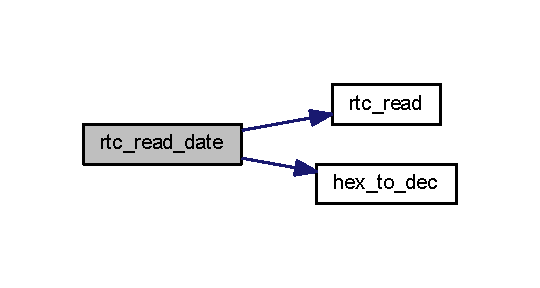
\includegraphics[width=259pt]{group__rtc_ga83dbab748017bcc8531622b94cca1be1_cgraph}
\end{center}
\end{figure}
\hypertarget{group__rtc_ga3b9f4583bad77c33ea0e82c1c1ad5305}{}\label{group__rtc_ga3b9f4583bad77c33ea0e82c1c1ad5305} 
\index{rtc@{rtc}!rtc\+\_\+subscribe\+\_\+int@{rtc\+\_\+subscribe\+\_\+int}}
\index{rtc\+\_\+subscribe\+\_\+int@{rtc\+\_\+subscribe\+\_\+int}!rtc@{rtc}}
\subsubsection{\texorpdfstring{rtc\+\_\+subscribe\+\_\+int()}{rtc\_subscribe\_int()}}
{\footnotesize\ttfamily int rtc\+\_\+subscribe\+\_\+int (\begin{DoxyParamCaption}\item[{unsigned int $\ast$}]{rtc\+\_\+hook\+\_\+id }\end{DoxyParamCaption})}



subscribes a R\+TC interruption 


\begin{DoxyParams}{Parameters}
{\em rtc\+\_\+hook\+\_\+id} & rtc hook\\
\hline
\end{DoxyParams}
\begin{DoxyReturn}{Returns}
Return 0 upon success and non-\/zero otherwise 
\end{DoxyReturn}
\hypertarget{group__rtc_ga61932ec1f55303bac55dea276d2a141f}{}\label{group__rtc_ga61932ec1f55303bac55dea276d2a141f} 
\index{rtc@{rtc}!rtc\+\_\+unsubscribe\+\_\+int@{rtc\+\_\+unsubscribe\+\_\+int}}
\index{rtc\+\_\+unsubscribe\+\_\+int@{rtc\+\_\+unsubscribe\+\_\+int}!rtc@{rtc}}
\subsubsection{\texorpdfstring{rtc\+\_\+unsubscribe\+\_\+int()}{rtc\_unsubscribe\_int()}}
{\footnotesize\ttfamily int rtc\+\_\+unsubscribe\+\_\+int (\begin{DoxyParamCaption}\item[{unsigned int $\ast$}]{rtc\+\_\+hook\+\_\+id }\end{DoxyParamCaption})}



unsubscribes a R\+TC interruption 


\begin{DoxyParams}{Parameters}
{\em rtc\+\_\+hook\+\_\+id} & rtc hook\\
\hline
\end{DoxyParams}
\begin{DoxyReturn}{Returns}
Return 0 upon success and non-\/zero otherwise 
\end{DoxyReturn}

\hypertarget{group__ser__port}{}\section{ser\+\_\+port}
\label{group__ser__port}\index{ser\+\_\+port@{ser\+\_\+port}}
\subsection*{Data Structures}
\begin{DoxyCompactItemize}
\item 
struct \hyperlink{structser__conf__t}{ser\+\_\+conf\+\_\+t}
\end{DoxyCompactItemize}
\subsection*{Macros}
\begin{DoxyCompactItemize}
\item 
\#define \hyperlink{group__ser__port_ga3a8ea58898cb58fc96013383d39f482c}{B\+IT}(n)~(0x01$<$$<$(n))
\item 
\#define \hyperlink{group__ser__port_ga98199cd85fbe47b9a741b07762260422}{S\+E\+R\+\_\+\+C\+O\+M1\+\_\+\+A\+D\+DR}~0x3\+F8
\item 
\#define \hyperlink{group__ser__port_ga62c7a28d9eaa93631e7bb202f91dddcf}{S\+E\+R\+\_\+\+C\+O\+M2\+\_\+\+A\+D\+DR}~0x2\+F8
\item 
\#define \hyperlink{group__ser__port_gaf0ec610995d060379690114f01c6eeaf}{S\+E\+R\+\_\+\+C\+O\+M1\+\_\+\+I\+RQ}~4
\item 
\#define \hyperlink{group__ser__port_ga420c631d8b538f2a8058e793523149e2}{S\+E\+R\+\_\+\+C\+O\+M2\+\_\+\+I\+RQ}~3
\item 
\#define \hyperlink{group__ser__port_ga673bc80505f70c750fe685caf9a0d6b0}{S\+E\+R\+\_\+\+H\+O\+OK}~5
\item 
\#define \hyperlink{group__ser__port_ga1a522aa19bcb695a9df30032a893bee3}{D\+E\+L\+A\+Y\+\_\+\+US}~20000
\end{DoxyCompactItemize}
\subsection*{Functions}
\begin{DoxyCompactItemize}
\item 
\hyperlink{structser__conf__t}{ser\+\_\+conf\+\_\+t} \hyperlink{group__ser__port_gad7f306574426f807f460ddcde260c11b}{get\+\_\+conf} (unsigned short base\+\_\+addr)
\begin{DoxyCompactList}\small\item\em This function gets the configuration of an U\+A\+RT register. \end{DoxyCompactList}\item 
int \hyperlink{group__ser__port_ga03bc33099d89326fb9a26cc0fef1cc7a}{ser\+\_\+set\+\_\+bits\+\_\+per\+\_\+char} (unsigned short base\+\_\+addr, int bits)
\begin{DoxyCompactList}\small\item\em Sets the value of bits per character in the respective serial port. \end{DoxyCompactList}\item 
int \hyperlink{group__ser__port_ga7d67a8d80697182bb1afe90a65875c90}{ser\+\_\+set\+\_\+stop\+\_\+bits} (unsigned short base\+\_\+addr, int bits)
\begin{DoxyCompactList}\small\item\em Sets the value of bits per character in the respective serial port. \end{DoxyCompactList}\item 
int \hyperlink{group__ser__port_ga4a963c8e3cfb978a4e4a026add12483f}{ser\+\_\+set\+\_\+parity} (unsigned short base\+\_\+addr, int parity)
\begin{DoxyCompactList}\small\item\em Sets the value of bits per character in the respective serial port. \end{DoxyCompactList}\item 
int \hyperlink{group__ser__port_ga2b6153e7105a706ea7a331770150ac55}{ser\+\_\+set\+\_\+rate} (unsigned short base\+\_\+addr, int rate)
\begin{DoxyCompactList}\small\item\em Sets the value of bits per character in the respective serial port. \end{DoxyCompactList}\item 
int \hyperlink{group__ser__port_ga1e0894432789b7311021c4f862335065}{ser\+\_\+set\+\_\+conf} (unsigned short base\+\_\+addr, int bits, int stop, int parity, int rate)
\begin{DoxyCompactList}\small\item\em Sets the configuration of the serial port. \end{DoxyCompactList}\item 
int \hyperlink{group__ser__port_gaf51d56fa6069ce68bb9f34a1396b2ea1}{ser\+\_\+check\+\_\+lsr\+\_\+error} (unsigned short base\+\_\+addr)
\begin{DoxyCompactList}\small\item\em Checks if the lsr register has an error. \end{DoxyCompactList}\item 
int \hyperlink{group__ser__port_ga46bbb861095c5b7a44a33af5e19be100}{ser\+\_\+disable\+\_\+int} (unsigned short base\+\_\+addr)
\begin{DoxyCompactList}\small\item\em Disables I\+ER interrupts. \end{DoxyCompactList}\item 
int \hyperlink{group__ser__port_ga9ce4605b9346d093f446fa48b495406b}{ser\+\_\+send\+\_\+char\+\_\+poll} (unsigned short base\+\_\+addr, char c, int num\+\_\+cicles)
\begin{DoxyCompactList}\small\item\em transmits a char through the serial port \end{DoxyCompactList}\item 
int \hyperlink{group__ser__port_gae9c2959fb0c4f39b96c4621d985f5ed2}{ser\+\_\+receive\+\_\+char\+\_\+poll} (unsigned short base\+\_\+addr, unsigned long $\ast$c, int num\+\_\+cicles)
\begin{DoxyCompactList}\small\item\em receive a char through the serial port \end{DoxyCompactList}\end{DoxyCompactItemize}
\subsection*{R\+E\+G\+I\+S\+T\+ER}
\begin{DoxyCompactItemize}
\item 
\#define \hyperlink{group__ser__port_gaab10abea0297abdcf0aab7d7d0b5662f}{S\+E\+R\+\_\+\+R\+BR}~0
\item 
\#define \hyperlink{group__ser__port_ga3702c28928f73b9841ab8269f64177ed}{S\+E\+R\+\_\+\+T\+HR}~0
\item 
\#define \hyperlink{group__ser__port_ga783f8e3973a5f87d8af120d49742f834}{S\+E\+R\+\_\+\+I\+ER}~1
\item 
\#define \hyperlink{group__ser__port_ga483c46ea5ed36388947426211cb63eab}{S\+E\+R\+\_\+\+I\+IR}~2
\item 
\#define \hyperlink{group__ser__port_ga9261eef6859842b51e42894b61c5b1c0}{S\+E\+R\+\_\+\+F\+CR}~2
\item 
\#define \hyperlink{group__ser__port_ga6475db6ed9440a92c680e54b2912b191}{S\+E\+R\+\_\+\+L\+CR}~3
\item 
\#define \hyperlink{group__ser__port_ga0f21de7866d73161df9b492b415c370c}{S\+E\+R\+\_\+\+M\+CR}~4
\item 
\#define \hyperlink{group__ser__port_ga382b5d26eb113bfffbf2094eb4405042}{S\+E\+R\+\_\+\+L\+SR}~5
\item 
\#define \hyperlink{group__ser__port_gaf161670921d63a654492758b1998d222}{S\+E\+R\+\_\+\+M\+SR}~6
\item 
\#define \hyperlink{group__ser__port_ga0005836362c1dd009c7fe47720908b1b}{S\+E\+R\+\_\+\+SR}~7
\item 
\#define \hyperlink{group__ser__port_ga858484a29128b93600cd6b8971a91faf}{S\+E\+R\+\_\+\+D\+LL}~0
\item 
\#define \hyperlink{group__ser__port_ga54c2d9bcb790f3a6d0cd71d20ae5d427}{S\+E\+R\+\_\+\+D\+LM}~1
\item 
\#define \hyperlink{group__ser__port_ga2bce41e3ef0b59643bfc314fbdf89545}{S\+E\+R\+\_\+\+D\+L\+AB}~\hyperlink{video__gr_8c_a3a8ea58898cb58fc96013383d39f482c}{B\+IT}(7)
\end{DoxyCompactItemize}
\subsection*{S\+ER D\+A\+TA}
\begin{DoxyCompactItemize}
\item 
\#define \hyperlink{group__ser__port_gadf09d6c9cf68d22c596eb240a5febffb}{S\+E\+R\+\_\+\+D\+A\+TA}~0
\item 
\#define \hyperlink{group__ser__port_ga39627267c307802e2a030abe796fb97b}{S\+E\+R\+\_\+\+T\+X\+\_\+\+R\+DY}~(1$<$$<$5)
\item 
\#define \hyperlink{group__ser__port_ga3eb8525f2a4c6e405b2528526c71b0cf}{S\+E\+R\+\_\+\+R\+E\+C\+\_\+\+R\+DY}~\hyperlink{video__gr_8c_a3a8ea58898cb58fc96013383d39f482c}{B\+IT}(0)
\end{DoxyCompactItemize}
\subsection*{I\+ER}
\begin{DoxyCompactItemize}
\item 
\#define \hyperlink{group__ser__port_gafe8e1c08ba9763a976c8359d6f5b370b}{E\+N\+A\+B\+L\+E\+\_\+\+R\+E\+C\+\_\+\+I\+NT}~\hyperlink{video__gr_8c_a3a8ea58898cb58fc96013383d39f482c}{B\+IT}(0)
\item 
\#define \hyperlink{group__ser__port_gac33182192c6023fe0d50c63666551162}{E\+N\+A\+B\+L\+E\+\_\+\+T\+R\+A\+N\+S\+\_\+\+I\+NT}~\hyperlink{video__gr_8c_a3a8ea58898cb58fc96013383d39f482c}{B\+IT}(1)
\item 
\#define \hyperlink{group__ser__port_ga89361f04d2aef788b076d1ea455d5482}{E\+N\+A\+B\+L\+E\+\_\+\+L\+I\+N\+E\+\_\+\+S\+T\+A\+T\+U\+S\+\_\+\+I\+NT}~\hyperlink{video__gr_8c_a3a8ea58898cb58fc96013383d39f482c}{B\+IT}(2)
\end{DoxyCompactItemize}
\subsection*{E\+R\+R\+OR}
\begin{DoxyCompactItemize}
\item 
\#define \hyperlink{group__ser__port_gac22f7e8109686500cf878a26ea3af115}{S\+E\+R\+\_\+\+O\+V\+E\+R\+R\+U\+N\+\_\+\+E\+RR}~(1$<$$<$1)
\item 
\#define \hyperlink{group__ser__port_ga356ae2e9093b65d87b35a303f3092057}{S\+E\+R\+\_\+\+P\+A\+R\+I\+T\+Y\+\_\+\+E\+RR}~(1$<$$<$2)
\item 
\#define \hyperlink{group__ser__port_ga0182fcdfbfeb90906d60c3ddb411aece}{S\+E\+R\+\_\+\+F\+R\+A\+M\+E\+\_\+\+E\+RR}~(1$<$$<$3)
\end{DoxyCompactItemize}
\subsection*{F\+I\+FO}
\begin{DoxyCompactItemize}
\item 
\#define \hyperlink{group__ser__port_ga096773e56aa66b4b8721492e07c41c77}{S\+E\+R\+\_\+\+E\+N\+\_\+\+F\+I\+FO}~\hyperlink{video__gr_8c_a3a8ea58898cb58fc96013383d39f482c}{B\+IT}(0)
\item 
\#define \hyperlink{group__ser__port_ga3b73c7fc2c9e1534d663a7b8c588240a}{S\+E\+R\+\_\+\+C\+L\+R\+\_\+\+R\+E\+C\+\_\+\+F\+I\+FO}~\hyperlink{video__gr_8c_a3a8ea58898cb58fc96013383d39f482c}{B\+IT}(1)
\item 
\#define \hyperlink{group__ser__port_ga565f202296c0e98389a04cf981110b2a}{S\+E\+R\+\_\+\+C\+L\+R\+\_\+\+T\+R\+A\+N\+S\+\_\+\+F\+I\+FO}~\hyperlink{video__gr_8c_a3a8ea58898cb58fc96013383d39f482c}{B\+IT}(2)
\item 
\#define \hyperlink{group__ser__port_ga4c5703803ba2f88b2c80a98503cd7b48}{S\+E\+R\+\_\+\+T\+R\+I\+G\+G\+ER}~\hyperlink{video__gr_8c_a3a8ea58898cb58fc96013383d39f482c}{B\+IT}(7)
\end{DoxyCompactItemize}
\subsection*{I\+IR}
\begin{DoxyCompactItemize}
\item 
\#define \hyperlink{group__ser__port_ga92820a610e36c919d8a8cb2bb731e43e}{S\+E\+R\+\_\+\+I\+N\+T\+\_\+\+O\+RG}~\hyperlink{video__gr_8c_a3a8ea58898cb58fc96013383d39f482c}{B\+IT}(3) $\vert$ \hyperlink{video__gr_8c_a3a8ea58898cb58fc96013383d39f482c}{B\+IT}(2) $\vert$\hyperlink{video__gr_8c_a3a8ea58898cb58fc96013383d39f482c}{B\+IT}(1)
\item 
\#define \hyperlink{group__ser__port_ga7685f0a713a489943c06459e830d7a86}{S\+E\+R\+\_\+\+I\+N\+T\+\_\+\+S\+T\+A\+T\+US}~\hyperlink{video__gr_8c_a3a8ea58898cb58fc96013383d39f482c}{B\+IT}(0)
\item 
\#define \hyperlink{group__ser__port_ga9cc69bb601e83e6539168370d49c71a5}{S\+E\+R\+\_\+\+I\+N\+T\+\_\+\+L\+I\+N\+E\+\_\+\+S\+T\+A\+T\+US}~(\hyperlink{video__gr_8c_a3a8ea58898cb58fc96013383d39f482c}{B\+IT}(2) $\vert$\hyperlink{video__gr_8c_a3a8ea58898cb58fc96013383d39f482c}{B\+IT}(1))
\item 
\#define \hyperlink{group__ser__port_gaa9a2bde6c86a448c7e5b3f2abd691da7}{S\+E\+R\+\_\+\+I\+N\+T\+\_\+\+T\+R\+A\+N\+S\+\_\+\+E\+M\+P\+TY}~\hyperlink{video__gr_8c_a3a8ea58898cb58fc96013383d39f482c}{B\+IT}(1)
\item 
\#define \hyperlink{group__ser__port_gad3a9fdeed634179f19f0fb175150faab}{S\+E\+R\+\_\+\+I\+N\+T\+\_\+\+R\+E\+C\+\_\+\+D\+A\+T\+A\+\_\+\+A\+V\+LB}~\hyperlink{video__gr_8c_a3a8ea58898cb58fc96013383d39f482c}{B\+IT}(2)
\end{DoxyCompactItemize}


\subsection{Detailed Description}
Functions for serial port 

\subsection{Macro Definition Documentation}
\hypertarget{group__ser__port_ga3a8ea58898cb58fc96013383d39f482c}{}\label{group__ser__port_ga3a8ea58898cb58fc96013383d39f482c} 
\index{ser\+\_\+port@{ser\+\_\+port}!B\+IT@{B\+IT}}
\index{B\+IT@{B\+IT}!ser\+\_\+port@{ser\+\_\+port}}
\subsubsection{\texorpdfstring{B\+IT}{BIT}}
{\footnotesize\ttfamily \#define B\+IT(\begin{DoxyParamCaption}\item[{}]{n }\end{DoxyParamCaption})~(0x01$<$$<$(n))}

\hypertarget{group__ser__port_ga1a522aa19bcb695a9df30032a893bee3}{}\label{group__ser__port_ga1a522aa19bcb695a9df30032a893bee3} 
\index{ser\+\_\+port@{ser\+\_\+port}!D\+E\+L\+A\+Y\+\_\+\+US@{D\+E\+L\+A\+Y\+\_\+\+US}}
\index{D\+E\+L\+A\+Y\+\_\+\+US@{D\+E\+L\+A\+Y\+\_\+\+US}!ser\+\_\+port@{ser\+\_\+port}}
\subsubsection{\texorpdfstring{D\+E\+L\+A\+Y\+\_\+\+US}{DELAY\_US}}
{\footnotesize\ttfamily \#define D\+E\+L\+A\+Y\+\_\+\+US~20000}

\hypertarget{group__ser__port_ga89361f04d2aef788b076d1ea455d5482}{}\label{group__ser__port_ga89361f04d2aef788b076d1ea455d5482} 
\index{ser\+\_\+port@{ser\+\_\+port}!E\+N\+A\+B\+L\+E\+\_\+\+L\+I\+N\+E\+\_\+\+S\+T\+A\+T\+U\+S\+\_\+\+I\+NT@{E\+N\+A\+B\+L\+E\+\_\+\+L\+I\+N\+E\+\_\+\+S\+T\+A\+T\+U\+S\+\_\+\+I\+NT}}
\index{E\+N\+A\+B\+L\+E\+\_\+\+L\+I\+N\+E\+\_\+\+S\+T\+A\+T\+U\+S\+\_\+\+I\+NT@{E\+N\+A\+B\+L\+E\+\_\+\+L\+I\+N\+E\+\_\+\+S\+T\+A\+T\+U\+S\+\_\+\+I\+NT}!ser\+\_\+port@{ser\+\_\+port}}
\subsubsection{\texorpdfstring{E\+N\+A\+B\+L\+E\+\_\+\+L\+I\+N\+E\+\_\+\+S\+T\+A\+T\+U\+S\+\_\+\+I\+NT}{ENABLE\_LINE\_STATUS\_INT}}
{\footnotesize\ttfamily \#define E\+N\+A\+B\+L\+E\+\_\+\+L\+I\+N\+E\+\_\+\+S\+T\+A\+T\+U\+S\+\_\+\+I\+NT~\hyperlink{video__gr_8c_a3a8ea58898cb58fc96013383d39f482c}{B\+IT}(2)}

\hypertarget{group__ser__port_gafe8e1c08ba9763a976c8359d6f5b370b}{}\label{group__ser__port_gafe8e1c08ba9763a976c8359d6f5b370b} 
\index{ser\+\_\+port@{ser\+\_\+port}!E\+N\+A\+B\+L\+E\+\_\+\+R\+E\+C\+\_\+\+I\+NT@{E\+N\+A\+B\+L\+E\+\_\+\+R\+E\+C\+\_\+\+I\+NT}}
\index{E\+N\+A\+B\+L\+E\+\_\+\+R\+E\+C\+\_\+\+I\+NT@{E\+N\+A\+B\+L\+E\+\_\+\+R\+E\+C\+\_\+\+I\+NT}!ser\+\_\+port@{ser\+\_\+port}}
\subsubsection{\texorpdfstring{E\+N\+A\+B\+L\+E\+\_\+\+R\+E\+C\+\_\+\+I\+NT}{ENABLE\_REC\_INT}}
{\footnotesize\ttfamily \#define E\+N\+A\+B\+L\+E\+\_\+\+R\+E\+C\+\_\+\+I\+NT~\hyperlink{video__gr_8c_a3a8ea58898cb58fc96013383d39f482c}{B\+IT}(0)}

\hypertarget{group__ser__port_gac33182192c6023fe0d50c63666551162}{}\label{group__ser__port_gac33182192c6023fe0d50c63666551162} 
\index{ser\+\_\+port@{ser\+\_\+port}!E\+N\+A\+B\+L\+E\+\_\+\+T\+R\+A\+N\+S\+\_\+\+I\+NT@{E\+N\+A\+B\+L\+E\+\_\+\+T\+R\+A\+N\+S\+\_\+\+I\+NT}}
\index{E\+N\+A\+B\+L\+E\+\_\+\+T\+R\+A\+N\+S\+\_\+\+I\+NT@{E\+N\+A\+B\+L\+E\+\_\+\+T\+R\+A\+N\+S\+\_\+\+I\+NT}!ser\+\_\+port@{ser\+\_\+port}}
\subsubsection{\texorpdfstring{E\+N\+A\+B\+L\+E\+\_\+\+T\+R\+A\+N\+S\+\_\+\+I\+NT}{ENABLE\_TRANS\_INT}}
{\footnotesize\ttfamily \#define E\+N\+A\+B\+L\+E\+\_\+\+T\+R\+A\+N\+S\+\_\+\+I\+NT~\hyperlink{video__gr_8c_a3a8ea58898cb58fc96013383d39f482c}{B\+IT}(1)}

\hypertarget{group__ser__port_ga3b73c7fc2c9e1534d663a7b8c588240a}{}\label{group__ser__port_ga3b73c7fc2c9e1534d663a7b8c588240a} 
\index{ser\+\_\+port@{ser\+\_\+port}!S\+E\+R\+\_\+\+C\+L\+R\+\_\+\+R\+E\+C\+\_\+\+F\+I\+FO@{S\+E\+R\+\_\+\+C\+L\+R\+\_\+\+R\+E\+C\+\_\+\+F\+I\+FO}}
\index{S\+E\+R\+\_\+\+C\+L\+R\+\_\+\+R\+E\+C\+\_\+\+F\+I\+FO@{S\+E\+R\+\_\+\+C\+L\+R\+\_\+\+R\+E\+C\+\_\+\+F\+I\+FO}!ser\+\_\+port@{ser\+\_\+port}}
\subsubsection{\texorpdfstring{S\+E\+R\+\_\+\+C\+L\+R\+\_\+\+R\+E\+C\+\_\+\+F\+I\+FO}{SER\_CLR\_REC\_FIFO}}
{\footnotesize\ttfamily \#define S\+E\+R\+\_\+\+C\+L\+R\+\_\+\+R\+E\+C\+\_\+\+F\+I\+FO~\hyperlink{video__gr_8c_a3a8ea58898cb58fc96013383d39f482c}{B\+IT}(1)}

\hypertarget{group__ser__port_ga565f202296c0e98389a04cf981110b2a}{}\label{group__ser__port_ga565f202296c0e98389a04cf981110b2a} 
\index{ser\+\_\+port@{ser\+\_\+port}!S\+E\+R\+\_\+\+C\+L\+R\+\_\+\+T\+R\+A\+N\+S\+\_\+\+F\+I\+FO@{S\+E\+R\+\_\+\+C\+L\+R\+\_\+\+T\+R\+A\+N\+S\+\_\+\+F\+I\+FO}}
\index{S\+E\+R\+\_\+\+C\+L\+R\+\_\+\+T\+R\+A\+N\+S\+\_\+\+F\+I\+FO@{S\+E\+R\+\_\+\+C\+L\+R\+\_\+\+T\+R\+A\+N\+S\+\_\+\+F\+I\+FO}!ser\+\_\+port@{ser\+\_\+port}}
\subsubsection{\texorpdfstring{S\+E\+R\+\_\+\+C\+L\+R\+\_\+\+T\+R\+A\+N\+S\+\_\+\+F\+I\+FO}{SER\_CLR\_TRANS\_FIFO}}
{\footnotesize\ttfamily \#define S\+E\+R\+\_\+\+C\+L\+R\+\_\+\+T\+R\+A\+N\+S\+\_\+\+F\+I\+FO~\hyperlink{video__gr_8c_a3a8ea58898cb58fc96013383d39f482c}{B\+IT}(2)}

\hypertarget{group__ser__port_ga98199cd85fbe47b9a741b07762260422}{}\label{group__ser__port_ga98199cd85fbe47b9a741b07762260422} 
\index{ser\+\_\+port@{ser\+\_\+port}!S\+E\+R\+\_\+\+C\+O\+M1\+\_\+\+A\+D\+DR@{S\+E\+R\+\_\+\+C\+O\+M1\+\_\+\+A\+D\+DR}}
\index{S\+E\+R\+\_\+\+C\+O\+M1\+\_\+\+A\+D\+DR@{S\+E\+R\+\_\+\+C\+O\+M1\+\_\+\+A\+D\+DR}!ser\+\_\+port@{ser\+\_\+port}}
\subsubsection{\texorpdfstring{S\+E\+R\+\_\+\+C\+O\+M1\+\_\+\+A\+D\+DR}{SER\_COM1\_ADDR}}
{\footnotesize\ttfamily \#define S\+E\+R\+\_\+\+C\+O\+M1\+\_\+\+A\+D\+DR~0x3\+F8}

\hypertarget{group__ser__port_gaf0ec610995d060379690114f01c6eeaf}{}\label{group__ser__port_gaf0ec610995d060379690114f01c6eeaf} 
\index{ser\+\_\+port@{ser\+\_\+port}!S\+E\+R\+\_\+\+C\+O\+M1\+\_\+\+I\+RQ@{S\+E\+R\+\_\+\+C\+O\+M1\+\_\+\+I\+RQ}}
\index{S\+E\+R\+\_\+\+C\+O\+M1\+\_\+\+I\+RQ@{S\+E\+R\+\_\+\+C\+O\+M1\+\_\+\+I\+RQ}!ser\+\_\+port@{ser\+\_\+port}}
\subsubsection{\texorpdfstring{S\+E\+R\+\_\+\+C\+O\+M1\+\_\+\+I\+RQ}{SER\_COM1\_IRQ}}
{\footnotesize\ttfamily \#define S\+E\+R\+\_\+\+C\+O\+M1\+\_\+\+I\+RQ~4}

\hypertarget{group__ser__port_ga62c7a28d9eaa93631e7bb202f91dddcf}{}\label{group__ser__port_ga62c7a28d9eaa93631e7bb202f91dddcf} 
\index{ser\+\_\+port@{ser\+\_\+port}!S\+E\+R\+\_\+\+C\+O\+M2\+\_\+\+A\+D\+DR@{S\+E\+R\+\_\+\+C\+O\+M2\+\_\+\+A\+D\+DR}}
\index{S\+E\+R\+\_\+\+C\+O\+M2\+\_\+\+A\+D\+DR@{S\+E\+R\+\_\+\+C\+O\+M2\+\_\+\+A\+D\+DR}!ser\+\_\+port@{ser\+\_\+port}}
\subsubsection{\texorpdfstring{S\+E\+R\+\_\+\+C\+O\+M2\+\_\+\+A\+D\+DR}{SER\_COM2\_ADDR}}
{\footnotesize\ttfamily \#define S\+E\+R\+\_\+\+C\+O\+M2\+\_\+\+A\+D\+DR~0x2\+F8}

\hypertarget{group__ser__port_ga420c631d8b538f2a8058e793523149e2}{}\label{group__ser__port_ga420c631d8b538f2a8058e793523149e2} 
\index{ser\+\_\+port@{ser\+\_\+port}!S\+E\+R\+\_\+\+C\+O\+M2\+\_\+\+I\+RQ@{S\+E\+R\+\_\+\+C\+O\+M2\+\_\+\+I\+RQ}}
\index{S\+E\+R\+\_\+\+C\+O\+M2\+\_\+\+I\+RQ@{S\+E\+R\+\_\+\+C\+O\+M2\+\_\+\+I\+RQ}!ser\+\_\+port@{ser\+\_\+port}}
\subsubsection{\texorpdfstring{S\+E\+R\+\_\+\+C\+O\+M2\+\_\+\+I\+RQ}{SER\_COM2\_IRQ}}
{\footnotesize\ttfamily \#define S\+E\+R\+\_\+\+C\+O\+M2\+\_\+\+I\+RQ~3}

\hypertarget{group__ser__port_gadf09d6c9cf68d22c596eb240a5febffb}{}\label{group__ser__port_gadf09d6c9cf68d22c596eb240a5febffb} 
\index{ser\+\_\+port@{ser\+\_\+port}!S\+E\+R\+\_\+\+D\+A\+TA@{S\+E\+R\+\_\+\+D\+A\+TA}}
\index{S\+E\+R\+\_\+\+D\+A\+TA@{S\+E\+R\+\_\+\+D\+A\+TA}!ser\+\_\+port@{ser\+\_\+port}}
\subsubsection{\texorpdfstring{S\+E\+R\+\_\+\+D\+A\+TA}{SER\_DATA}}
{\footnotesize\ttfamily \#define S\+E\+R\+\_\+\+D\+A\+TA~0}

\hypertarget{group__ser__port_ga2bce41e3ef0b59643bfc314fbdf89545}{}\label{group__ser__port_ga2bce41e3ef0b59643bfc314fbdf89545} 
\index{ser\+\_\+port@{ser\+\_\+port}!S\+E\+R\+\_\+\+D\+L\+AB@{S\+E\+R\+\_\+\+D\+L\+AB}}
\index{S\+E\+R\+\_\+\+D\+L\+AB@{S\+E\+R\+\_\+\+D\+L\+AB}!ser\+\_\+port@{ser\+\_\+port}}
\subsubsection{\texorpdfstring{S\+E\+R\+\_\+\+D\+L\+AB}{SER\_DLAB}}
{\footnotesize\ttfamily \#define S\+E\+R\+\_\+\+D\+L\+AB~\hyperlink{video__gr_8c_a3a8ea58898cb58fc96013383d39f482c}{B\+IT}(7)}

\hypertarget{group__ser__port_ga858484a29128b93600cd6b8971a91faf}{}\label{group__ser__port_ga858484a29128b93600cd6b8971a91faf} 
\index{ser\+\_\+port@{ser\+\_\+port}!S\+E\+R\+\_\+\+D\+LL@{S\+E\+R\+\_\+\+D\+LL}}
\index{S\+E\+R\+\_\+\+D\+LL@{S\+E\+R\+\_\+\+D\+LL}!ser\+\_\+port@{ser\+\_\+port}}
\subsubsection{\texorpdfstring{S\+E\+R\+\_\+\+D\+LL}{SER\_DLL}}
{\footnotesize\ttfamily \#define S\+E\+R\+\_\+\+D\+LL~0}

\hypertarget{group__ser__port_ga54c2d9bcb790f3a6d0cd71d20ae5d427}{}\label{group__ser__port_ga54c2d9bcb790f3a6d0cd71d20ae5d427} 
\index{ser\+\_\+port@{ser\+\_\+port}!S\+E\+R\+\_\+\+D\+LM@{S\+E\+R\+\_\+\+D\+LM}}
\index{S\+E\+R\+\_\+\+D\+LM@{S\+E\+R\+\_\+\+D\+LM}!ser\+\_\+port@{ser\+\_\+port}}
\subsubsection{\texorpdfstring{S\+E\+R\+\_\+\+D\+LM}{SER\_DLM}}
{\footnotesize\ttfamily \#define S\+E\+R\+\_\+\+D\+LM~1}

\hypertarget{group__ser__port_ga096773e56aa66b4b8721492e07c41c77}{}\label{group__ser__port_ga096773e56aa66b4b8721492e07c41c77} 
\index{ser\+\_\+port@{ser\+\_\+port}!S\+E\+R\+\_\+\+E\+N\+\_\+\+F\+I\+FO@{S\+E\+R\+\_\+\+E\+N\+\_\+\+F\+I\+FO}}
\index{S\+E\+R\+\_\+\+E\+N\+\_\+\+F\+I\+FO@{S\+E\+R\+\_\+\+E\+N\+\_\+\+F\+I\+FO}!ser\+\_\+port@{ser\+\_\+port}}
\subsubsection{\texorpdfstring{S\+E\+R\+\_\+\+E\+N\+\_\+\+F\+I\+FO}{SER\_EN\_FIFO}}
{\footnotesize\ttfamily \#define S\+E\+R\+\_\+\+E\+N\+\_\+\+F\+I\+FO~\hyperlink{video__gr_8c_a3a8ea58898cb58fc96013383d39f482c}{B\+IT}(0)}

\hypertarget{group__ser__port_ga9261eef6859842b51e42894b61c5b1c0}{}\label{group__ser__port_ga9261eef6859842b51e42894b61c5b1c0} 
\index{ser\+\_\+port@{ser\+\_\+port}!S\+E\+R\+\_\+\+F\+CR@{S\+E\+R\+\_\+\+F\+CR}}
\index{S\+E\+R\+\_\+\+F\+CR@{S\+E\+R\+\_\+\+F\+CR}!ser\+\_\+port@{ser\+\_\+port}}
\subsubsection{\texorpdfstring{S\+E\+R\+\_\+\+F\+CR}{SER\_FCR}}
{\footnotesize\ttfamily \#define S\+E\+R\+\_\+\+F\+CR~2}

\hypertarget{group__ser__port_ga0182fcdfbfeb90906d60c3ddb411aece}{}\label{group__ser__port_ga0182fcdfbfeb90906d60c3ddb411aece} 
\index{ser\+\_\+port@{ser\+\_\+port}!S\+E\+R\+\_\+\+F\+R\+A\+M\+E\+\_\+\+E\+RR@{S\+E\+R\+\_\+\+F\+R\+A\+M\+E\+\_\+\+E\+RR}}
\index{S\+E\+R\+\_\+\+F\+R\+A\+M\+E\+\_\+\+E\+RR@{S\+E\+R\+\_\+\+F\+R\+A\+M\+E\+\_\+\+E\+RR}!ser\+\_\+port@{ser\+\_\+port}}
\subsubsection{\texorpdfstring{S\+E\+R\+\_\+\+F\+R\+A\+M\+E\+\_\+\+E\+RR}{SER\_FRAME\_ERR}}
{\footnotesize\ttfamily \#define S\+E\+R\+\_\+\+F\+R\+A\+M\+E\+\_\+\+E\+RR~(1$<$$<$3)}

\hypertarget{group__ser__port_ga673bc80505f70c750fe685caf9a0d6b0}{}\label{group__ser__port_ga673bc80505f70c750fe685caf9a0d6b0} 
\index{ser\+\_\+port@{ser\+\_\+port}!S\+E\+R\+\_\+\+H\+O\+OK@{S\+E\+R\+\_\+\+H\+O\+OK}}
\index{S\+E\+R\+\_\+\+H\+O\+OK@{S\+E\+R\+\_\+\+H\+O\+OK}!ser\+\_\+port@{ser\+\_\+port}}
\subsubsection{\texorpdfstring{S\+E\+R\+\_\+\+H\+O\+OK}{SER\_HOOK}}
{\footnotesize\ttfamily \#define S\+E\+R\+\_\+\+H\+O\+OK~5}

\hypertarget{group__ser__port_ga783f8e3973a5f87d8af120d49742f834}{}\label{group__ser__port_ga783f8e3973a5f87d8af120d49742f834} 
\index{ser\+\_\+port@{ser\+\_\+port}!S\+E\+R\+\_\+\+I\+ER@{S\+E\+R\+\_\+\+I\+ER}}
\index{S\+E\+R\+\_\+\+I\+ER@{S\+E\+R\+\_\+\+I\+ER}!ser\+\_\+port@{ser\+\_\+port}}
\subsubsection{\texorpdfstring{S\+E\+R\+\_\+\+I\+ER}{SER\_IER}}
{\footnotesize\ttfamily \#define S\+E\+R\+\_\+\+I\+ER~1}

\hypertarget{group__ser__port_ga483c46ea5ed36388947426211cb63eab}{}\label{group__ser__port_ga483c46ea5ed36388947426211cb63eab} 
\index{ser\+\_\+port@{ser\+\_\+port}!S\+E\+R\+\_\+\+I\+IR@{S\+E\+R\+\_\+\+I\+IR}}
\index{S\+E\+R\+\_\+\+I\+IR@{S\+E\+R\+\_\+\+I\+IR}!ser\+\_\+port@{ser\+\_\+port}}
\subsubsection{\texorpdfstring{S\+E\+R\+\_\+\+I\+IR}{SER\_IIR}}
{\footnotesize\ttfamily \#define S\+E\+R\+\_\+\+I\+IR~2}

\hypertarget{group__ser__port_ga9cc69bb601e83e6539168370d49c71a5}{}\label{group__ser__port_ga9cc69bb601e83e6539168370d49c71a5} 
\index{ser\+\_\+port@{ser\+\_\+port}!S\+E\+R\+\_\+\+I\+N\+T\+\_\+\+L\+I\+N\+E\+\_\+\+S\+T\+A\+T\+US@{S\+E\+R\+\_\+\+I\+N\+T\+\_\+\+L\+I\+N\+E\+\_\+\+S\+T\+A\+T\+US}}
\index{S\+E\+R\+\_\+\+I\+N\+T\+\_\+\+L\+I\+N\+E\+\_\+\+S\+T\+A\+T\+US@{S\+E\+R\+\_\+\+I\+N\+T\+\_\+\+L\+I\+N\+E\+\_\+\+S\+T\+A\+T\+US}!ser\+\_\+port@{ser\+\_\+port}}
\subsubsection{\texorpdfstring{S\+E\+R\+\_\+\+I\+N\+T\+\_\+\+L\+I\+N\+E\+\_\+\+S\+T\+A\+T\+US}{SER\_INT\_LINE\_STATUS}}
{\footnotesize\ttfamily \#define S\+E\+R\+\_\+\+I\+N\+T\+\_\+\+L\+I\+N\+E\+\_\+\+S\+T\+A\+T\+US~(\hyperlink{video__gr_8c_a3a8ea58898cb58fc96013383d39f482c}{B\+IT}(2) $\vert$\hyperlink{video__gr_8c_a3a8ea58898cb58fc96013383d39f482c}{B\+IT}(1))}

\hypertarget{group__ser__port_ga92820a610e36c919d8a8cb2bb731e43e}{}\label{group__ser__port_ga92820a610e36c919d8a8cb2bb731e43e} 
\index{ser\+\_\+port@{ser\+\_\+port}!S\+E\+R\+\_\+\+I\+N\+T\+\_\+\+O\+RG@{S\+E\+R\+\_\+\+I\+N\+T\+\_\+\+O\+RG}}
\index{S\+E\+R\+\_\+\+I\+N\+T\+\_\+\+O\+RG@{S\+E\+R\+\_\+\+I\+N\+T\+\_\+\+O\+RG}!ser\+\_\+port@{ser\+\_\+port}}
\subsubsection{\texorpdfstring{S\+E\+R\+\_\+\+I\+N\+T\+\_\+\+O\+RG}{SER\_INT\_ORG}}
{\footnotesize\ttfamily \#define S\+E\+R\+\_\+\+I\+N\+T\+\_\+\+O\+RG~\hyperlink{video__gr_8c_a3a8ea58898cb58fc96013383d39f482c}{B\+IT}(3) $\vert$ \hyperlink{video__gr_8c_a3a8ea58898cb58fc96013383d39f482c}{B\+IT}(2) $\vert$\hyperlink{video__gr_8c_a3a8ea58898cb58fc96013383d39f482c}{B\+IT}(1)}

\hypertarget{group__ser__port_gad3a9fdeed634179f19f0fb175150faab}{}\label{group__ser__port_gad3a9fdeed634179f19f0fb175150faab} 
\index{ser\+\_\+port@{ser\+\_\+port}!S\+E\+R\+\_\+\+I\+N\+T\+\_\+\+R\+E\+C\+\_\+\+D\+A\+T\+A\+\_\+\+A\+V\+LB@{S\+E\+R\+\_\+\+I\+N\+T\+\_\+\+R\+E\+C\+\_\+\+D\+A\+T\+A\+\_\+\+A\+V\+LB}}
\index{S\+E\+R\+\_\+\+I\+N\+T\+\_\+\+R\+E\+C\+\_\+\+D\+A\+T\+A\+\_\+\+A\+V\+LB@{S\+E\+R\+\_\+\+I\+N\+T\+\_\+\+R\+E\+C\+\_\+\+D\+A\+T\+A\+\_\+\+A\+V\+LB}!ser\+\_\+port@{ser\+\_\+port}}
\subsubsection{\texorpdfstring{S\+E\+R\+\_\+\+I\+N\+T\+\_\+\+R\+E\+C\+\_\+\+D\+A\+T\+A\+\_\+\+A\+V\+LB}{SER\_INT\_REC\_DATA\_AVLB}}
{\footnotesize\ttfamily \#define S\+E\+R\+\_\+\+I\+N\+T\+\_\+\+R\+E\+C\+\_\+\+D\+A\+T\+A\+\_\+\+A\+V\+LB~\hyperlink{video__gr_8c_a3a8ea58898cb58fc96013383d39f482c}{B\+IT}(2)}

\hypertarget{group__ser__port_ga7685f0a713a489943c06459e830d7a86}{}\label{group__ser__port_ga7685f0a713a489943c06459e830d7a86} 
\index{ser\+\_\+port@{ser\+\_\+port}!S\+E\+R\+\_\+\+I\+N\+T\+\_\+\+S\+T\+A\+T\+US@{S\+E\+R\+\_\+\+I\+N\+T\+\_\+\+S\+T\+A\+T\+US}}
\index{S\+E\+R\+\_\+\+I\+N\+T\+\_\+\+S\+T\+A\+T\+US@{S\+E\+R\+\_\+\+I\+N\+T\+\_\+\+S\+T\+A\+T\+US}!ser\+\_\+port@{ser\+\_\+port}}
\subsubsection{\texorpdfstring{S\+E\+R\+\_\+\+I\+N\+T\+\_\+\+S\+T\+A\+T\+US}{SER\_INT\_STATUS}}
{\footnotesize\ttfamily \#define S\+E\+R\+\_\+\+I\+N\+T\+\_\+\+S\+T\+A\+T\+US~\hyperlink{video__gr_8c_a3a8ea58898cb58fc96013383d39f482c}{B\+IT}(0)}

\hypertarget{group__ser__port_gaa9a2bde6c86a448c7e5b3f2abd691da7}{}\label{group__ser__port_gaa9a2bde6c86a448c7e5b3f2abd691da7} 
\index{ser\+\_\+port@{ser\+\_\+port}!S\+E\+R\+\_\+\+I\+N\+T\+\_\+\+T\+R\+A\+N\+S\+\_\+\+E\+M\+P\+TY@{S\+E\+R\+\_\+\+I\+N\+T\+\_\+\+T\+R\+A\+N\+S\+\_\+\+E\+M\+P\+TY}}
\index{S\+E\+R\+\_\+\+I\+N\+T\+\_\+\+T\+R\+A\+N\+S\+\_\+\+E\+M\+P\+TY@{S\+E\+R\+\_\+\+I\+N\+T\+\_\+\+T\+R\+A\+N\+S\+\_\+\+E\+M\+P\+TY}!ser\+\_\+port@{ser\+\_\+port}}
\subsubsection{\texorpdfstring{S\+E\+R\+\_\+\+I\+N\+T\+\_\+\+T\+R\+A\+N\+S\+\_\+\+E\+M\+P\+TY}{SER\_INT\_TRANS\_EMPTY}}
{\footnotesize\ttfamily \#define S\+E\+R\+\_\+\+I\+N\+T\+\_\+\+T\+R\+A\+N\+S\+\_\+\+E\+M\+P\+TY~\hyperlink{video__gr_8c_a3a8ea58898cb58fc96013383d39f482c}{B\+IT}(1)}

\hypertarget{group__ser__port_ga6475db6ed9440a92c680e54b2912b191}{}\label{group__ser__port_ga6475db6ed9440a92c680e54b2912b191} 
\index{ser\+\_\+port@{ser\+\_\+port}!S\+E\+R\+\_\+\+L\+CR@{S\+E\+R\+\_\+\+L\+CR}}
\index{S\+E\+R\+\_\+\+L\+CR@{S\+E\+R\+\_\+\+L\+CR}!ser\+\_\+port@{ser\+\_\+port}}
\subsubsection{\texorpdfstring{S\+E\+R\+\_\+\+L\+CR}{SER\_LCR}}
{\footnotesize\ttfamily \#define S\+E\+R\+\_\+\+L\+CR~3}

\hypertarget{group__ser__port_ga382b5d26eb113bfffbf2094eb4405042}{}\label{group__ser__port_ga382b5d26eb113bfffbf2094eb4405042} 
\index{ser\+\_\+port@{ser\+\_\+port}!S\+E\+R\+\_\+\+L\+SR@{S\+E\+R\+\_\+\+L\+SR}}
\index{S\+E\+R\+\_\+\+L\+SR@{S\+E\+R\+\_\+\+L\+SR}!ser\+\_\+port@{ser\+\_\+port}}
\subsubsection{\texorpdfstring{S\+E\+R\+\_\+\+L\+SR}{SER\_LSR}}
{\footnotesize\ttfamily \#define S\+E\+R\+\_\+\+L\+SR~5}

\hypertarget{group__ser__port_ga0f21de7866d73161df9b492b415c370c}{}\label{group__ser__port_ga0f21de7866d73161df9b492b415c370c} 
\index{ser\+\_\+port@{ser\+\_\+port}!S\+E\+R\+\_\+\+M\+CR@{S\+E\+R\+\_\+\+M\+CR}}
\index{S\+E\+R\+\_\+\+M\+CR@{S\+E\+R\+\_\+\+M\+CR}!ser\+\_\+port@{ser\+\_\+port}}
\subsubsection{\texorpdfstring{S\+E\+R\+\_\+\+M\+CR}{SER\_MCR}}
{\footnotesize\ttfamily \#define S\+E\+R\+\_\+\+M\+CR~4}

\hypertarget{group__ser__port_gaf161670921d63a654492758b1998d222}{}\label{group__ser__port_gaf161670921d63a654492758b1998d222} 
\index{ser\+\_\+port@{ser\+\_\+port}!S\+E\+R\+\_\+\+M\+SR@{S\+E\+R\+\_\+\+M\+SR}}
\index{S\+E\+R\+\_\+\+M\+SR@{S\+E\+R\+\_\+\+M\+SR}!ser\+\_\+port@{ser\+\_\+port}}
\subsubsection{\texorpdfstring{S\+E\+R\+\_\+\+M\+SR}{SER\_MSR}}
{\footnotesize\ttfamily \#define S\+E\+R\+\_\+\+M\+SR~6}

\hypertarget{group__ser__port_gac22f7e8109686500cf878a26ea3af115}{}\label{group__ser__port_gac22f7e8109686500cf878a26ea3af115} 
\index{ser\+\_\+port@{ser\+\_\+port}!S\+E\+R\+\_\+\+O\+V\+E\+R\+R\+U\+N\+\_\+\+E\+RR@{S\+E\+R\+\_\+\+O\+V\+E\+R\+R\+U\+N\+\_\+\+E\+RR}}
\index{S\+E\+R\+\_\+\+O\+V\+E\+R\+R\+U\+N\+\_\+\+E\+RR@{S\+E\+R\+\_\+\+O\+V\+E\+R\+R\+U\+N\+\_\+\+E\+RR}!ser\+\_\+port@{ser\+\_\+port}}
\subsubsection{\texorpdfstring{S\+E\+R\+\_\+\+O\+V\+E\+R\+R\+U\+N\+\_\+\+E\+RR}{SER\_OVERRUN\_ERR}}
{\footnotesize\ttfamily \#define S\+E\+R\+\_\+\+O\+V\+E\+R\+R\+U\+N\+\_\+\+E\+RR~(1$<$$<$1)}

\hypertarget{group__ser__port_ga356ae2e9093b65d87b35a303f3092057}{}\label{group__ser__port_ga356ae2e9093b65d87b35a303f3092057} 
\index{ser\+\_\+port@{ser\+\_\+port}!S\+E\+R\+\_\+\+P\+A\+R\+I\+T\+Y\+\_\+\+E\+RR@{S\+E\+R\+\_\+\+P\+A\+R\+I\+T\+Y\+\_\+\+E\+RR}}
\index{S\+E\+R\+\_\+\+P\+A\+R\+I\+T\+Y\+\_\+\+E\+RR@{S\+E\+R\+\_\+\+P\+A\+R\+I\+T\+Y\+\_\+\+E\+RR}!ser\+\_\+port@{ser\+\_\+port}}
\subsubsection{\texorpdfstring{S\+E\+R\+\_\+\+P\+A\+R\+I\+T\+Y\+\_\+\+E\+RR}{SER\_PARITY\_ERR}}
{\footnotesize\ttfamily \#define S\+E\+R\+\_\+\+P\+A\+R\+I\+T\+Y\+\_\+\+E\+RR~(1$<$$<$2)}

\hypertarget{group__ser__port_gaab10abea0297abdcf0aab7d7d0b5662f}{}\label{group__ser__port_gaab10abea0297abdcf0aab7d7d0b5662f} 
\index{ser\+\_\+port@{ser\+\_\+port}!S\+E\+R\+\_\+\+R\+BR@{S\+E\+R\+\_\+\+R\+BR}}
\index{S\+E\+R\+\_\+\+R\+BR@{S\+E\+R\+\_\+\+R\+BR}!ser\+\_\+port@{ser\+\_\+port}}
\subsubsection{\texorpdfstring{S\+E\+R\+\_\+\+R\+BR}{SER\_RBR}}
{\footnotesize\ttfamily \#define S\+E\+R\+\_\+\+R\+BR~0}

\hypertarget{group__ser__port_ga3eb8525f2a4c6e405b2528526c71b0cf}{}\label{group__ser__port_ga3eb8525f2a4c6e405b2528526c71b0cf} 
\index{ser\+\_\+port@{ser\+\_\+port}!S\+E\+R\+\_\+\+R\+E\+C\+\_\+\+R\+DY@{S\+E\+R\+\_\+\+R\+E\+C\+\_\+\+R\+DY}}
\index{S\+E\+R\+\_\+\+R\+E\+C\+\_\+\+R\+DY@{S\+E\+R\+\_\+\+R\+E\+C\+\_\+\+R\+DY}!ser\+\_\+port@{ser\+\_\+port}}
\subsubsection{\texorpdfstring{S\+E\+R\+\_\+\+R\+E\+C\+\_\+\+R\+DY}{SER\_REC\_RDY}}
{\footnotesize\ttfamily \#define S\+E\+R\+\_\+\+R\+E\+C\+\_\+\+R\+DY~\hyperlink{video__gr_8c_a3a8ea58898cb58fc96013383d39f482c}{B\+IT}(0)}

\hypertarget{group__ser__port_ga0005836362c1dd009c7fe47720908b1b}{}\label{group__ser__port_ga0005836362c1dd009c7fe47720908b1b} 
\index{ser\+\_\+port@{ser\+\_\+port}!S\+E\+R\+\_\+\+SR@{S\+E\+R\+\_\+\+SR}}
\index{S\+E\+R\+\_\+\+SR@{S\+E\+R\+\_\+\+SR}!ser\+\_\+port@{ser\+\_\+port}}
\subsubsection{\texorpdfstring{S\+E\+R\+\_\+\+SR}{SER\_SR}}
{\footnotesize\ttfamily \#define S\+E\+R\+\_\+\+SR~7}

\hypertarget{group__ser__port_ga3702c28928f73b9841ab8269f64177ed}{}\label{group__ser__port_ga3702c28928f73b9841ab8269f64177ed} 
\index{ser\+\_\+port@{ser\+\_\+port}!S\+E\+R\+\_\+\+T\+HR@{S\+E\+R\+\_\+\+T\+HR}}
\index{S\+E\+R\+\_\+\+T\+HR@{S\+E\+R\+\_\+\+T\+HR}!ser\+\_\+port@{ser\+\_\+port}}
\subsubsection{\texorpdfstring{S\+E\+R\+\_\+\+T\+HR}{SER\_THR}}
{\footnotesize\ttfamily \#define S\+E\+R\+\_\+\+T\+HR~0}

\hypertarget{group__ser__port_ga4c5703803ba2f88b2c80a98503cd7b48}{}\label{group__ser__port_ga4c5703803ba2f88b2c80a98503cd7b48} 
\index{ser\+\_\+port@{ser\+\_\+port}!S\+E\+R\+\_\+\+T\+R\+I\+G\+G\+ER@{S\+E\+R\+\_\+\+T\+R\+I\+G\+G\+ER}}
\index{S\+E\+R\+\_\+\+T\+R\+I\+G\+G\+ER@{S\+E\+R\+\_\+\+T\+R\+I\+G\+G\+ER}!ser\+\_\+port@{ser\+\_\+port}}
\subsubsection{\texorpdfstring{S\+E\+R\+\_\+\+T\+R\+I\+G\+G\+ER}{SER\_TRIGGER}}
{\footnotesize\ttfamily \#define S\+E\+R\+\_\+\+T\+R\+I\+G\+G\+ER~\hyperlink{video__gr_8c_a3a8ea58898cb58fc96013383d39f482c}{B\+IT}(7)}

\hypertarget{group__ser__port_ga39627267c307802e2a030abe796fb97b}{}\label{group__ser__port_ga39627267c307802e2a030abe796fb97b} 
\index{ser\+\_\+port@{ser\+\_\+port}!S\+E\+R\+\_\+\+T\+X\+\_\+\+R\+DY@{S\+E\+R\+\_\+\+T\+X\+\_\+\+R\+DY}}
\index{S\+E\+R\+\_\+\+T\+X\+\_\+\+R\+DY@{S\+E\+R\+\_\+\+T\+X\+\_\+\+R\+DY}!ser\+\_\+port@{ser\+\_\+port}}
\subsubsection{\texorpdfstring{S\+E\+R\+\_\+\+T\+X\+\_\+\+R\+DY}{SER\_TX\_RDY}}
{\footnotesize\ttfamily \#define S\+E\+R\+\_\+\+T\+X\+\_\+\+R\+DY~(1$<$$<$5)}



\subsection{Function Documentation}
\hypertarget{group__ser__port_gad7f306574426f807f460ddcde260c11b}{}\label{group__ser__port_gad7f306574426f807f460ddcde260c11b} 
\index{ser\+\_\+port@{ser\+\_\+port}!get\+\_\+conf@{get\+\_\+conf}}
\index{get\+\_\+conf@{get\+\_\+conf}!ser\+\_\+port@{ser\+\_\+port}}
\subsubsection{\texorpdfstring{get\+\_\+conf()}{get\_conf()}}
{\footnotesize\ttfamily \hyperlink{structser__conf__t}{ser\+\_\+conf\+\_\+t} get\+\_\+conf (\begin{DoxyParamCaption}\item[{unsigned short}]{base\+\_\+addr }\end{DoxyParamCaption})}



This function gets the configuration of an U\+A\+RT register. 


\begin{DoxyParams}{Parameters}
{\em base\+\_\+addr} & address of of the serial port whose configuration we want to access\\
\hline
\end{DoxyParams}
\begin{DoxyReturn}{Returns}
configuration 
\end{DoxyReturn}
\hypertarget{group__ser__port_gaf51d56fa6069ce68bb9f34a1396b2ea1}{}\label{group__ser__port_gaf51d56fa6069ce68bb9f34a1396b2ea1} 
\index{ser\+\_\+port@{ser\+\_\+port}!ser\+\_\+check\+\_\+lsr\+\_\+error@{ser\+\_\+check\+\_\+lsr\+\_\+error}}
\index{ser\+\_\+check\+\_\+lsr\+\_\+error@{ser\+\_\+check\+\_\+lsr\+\_\+error}!ser\+\_\+port@{ser\+\_\+port}}
\subsubsection{\texorpdfstring{ser\+\_\+check\+\_\+lsr\+\_\+error()}{ser\_check\_lsr\_error()}}
{\footnotesize\ttfamily int ser\+\_\+check\+\_\+lsr\+\_\+error (\begin{DoxyParamCaption}\item[{unsigned short}]{base\+\_\+addr }\end{DoxyParamCaption})}



Checks if the lsr register has an error. 


\begin{DoxyParams}{Parameters}
{\em base\+\_\+addr} & address of the serial port whose configuration we want to change\\
\hline
\end{DoxyParams}
\begin{DoxyReturn}{Returns}
value 0 if there is no error, 1 if there and -\/1 if there was a problem obtaining the lsr error 
\end{DoxyReturn}
\hypertarget{group__ser__port_ga46bbb861095c5b7a44a33af5e19be100}{}\label{group__ser__port_ga46bbb861095c5b7a44a33af5e19be100} 
\index{ser\+\_\+port@{ser\+\_\+port}!ser\+\_\+disable\+\_\+int@{ser\+\_\+disable\+\_\+int}}
\index{ser\+\_\+disable\+\_\+int@{ser\+\_\+disable\+\_\+int}!ser\+\_\+port@{ser\+\_\+port}}
\subsubsection{\texorpdfstring{ser\+\_\+disable\+\_\+int()}{ser\_disable\_int()}}
{\footnotesize\ttfamily int ser\+\_\+disable\+\_\+int (\begin{DoxyParamCaption}\item[{unsigned short}]{base\+\_\+addr }\end{DoxyParamCaption})}



Disables I\+ER interrupts. 


\begin{DoxyParams}{Parameters}
{\em base\+\_\+addr} & address of the serial port whose configuration we want to change\\
\hline
\end{DoxyParams}
\begin{DoxyReturn}{Returns}
0 in case of success, 1 otherwise 
\end{DoxyReturn}
\hypertarget{group__ser__port_gae9c2959fb0c4f39b96c4621d985f5ed2}{}\label{group__ser__port_gae9c2959fb0c4f39b96c4621d985f5ed2} 
\index{ser\+\_\+port@{ser\+\_\+port}!ser\+\_\+receive\+\_\+char\+\_\+poll@{ser\+\_\+receive\+\_\+char\+\_\+poll}}
\index{ser\+\_\+receive\+\_\+char\+\_\+poll@{ser\+\_\+receive\+\_\+char\+\_\+poll}!ser\+\_\+port@{ser\+\_\+port}}
\subsubsection{\texorpdfstring{ser\+\_\+receive\+\_\+char\+\_\+poll()}{ser\_receive\_char\_poll()}}
{\footnotesize\ttfamily int ser\+\_\+receive\+\_\+char\+\_\+poll (\begin{DoxyParamCaption}\item[{unsigned short}]{base\+\_\+addr,  }\item[{unsigned long $\ast$}]{c,  }\item[{int}]{num\+\_\+cicles }\end{DoxyParamCaption})}



receive a char through the serial port 


\begin{DoxyParams}{Parameters}
{\em base\+\_\+addr} & -\/$>$ address of the serial port we want to use to change the character \\
\hline
{\em c} & -\/$>$ pointer to the variable that is going to store the character \\
\hline
{\em num\+\_\+cicles} & -\/$>$ maximum nnumber of cicles that the function will execute \\
\hline
\end{DoxyParams}
\begin{DoxyReturn}{Returns}
0 in case of success, 1 otherwise 
\end{DoxyReturn}
Here is the call graph for this function\+:\nopagebreak
\begin{figure}[H]
\begin{center}
\leavevmode
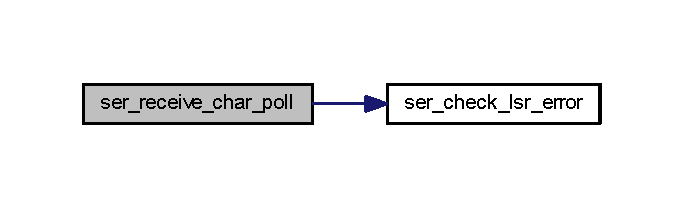
\includegraphics[width=328pt]{group__ser__port_gae9c2959fb0c4f39b96c4621d985f5ed2_cgraph}
\end{center}
\end{figure}
\hypertarget{group__ser__port_ga9ce4605b9346d093f446fa48b495406b}{}\label{group__ser__port_ga9ce4605b9346d093f446fa48b495406b} 
\index{ser\+\_\+port@{ser\+\_\+port}!ser\+\_\+send\+\_\+char\+\_\+poll@{ser\+\_\+send\+\_\+char\+\_\+poll}}
\index{ser\+\_\+send\+\_\+char\+\_\+poll@{ser\+\_\+send\+\_\+char\+\_\+poll}!ser\+\_\+port@{ser\+\_\+port}}
\subsubsection{\texorpdfstring{ser\+\_\+send\+\_\+char\+\_\+poll()}{ser\_send\_char\_poll()}}
{\footnotesize\ttfamily int ser\+\_\+send\+\_\+char\+\_\+poll (\begin{DoxyParamCaption}\item[{unsigned short}]{base\+\_\+addr,  }\item[{char}]{c,  }\item[{int}]{num\+\_\+cicles }\end{DoxyParamCaption})}



transmits a char through the serial port 


\begin{DoxyParams}{Parameters}
{\em base\+\_\+addr} & -\/$>$ address of the serial port we want to use to change the character \\
\hline
{\em c} & -\/$>$ character that we want to transmit \\
\hline
{\em num\+\_\+cicles} & -\/$>$ maximum number of cicles that the function will execute \\
\hline
\end{DoxyParams}
\begin{DoxyReturn}{Returns}
0 in case of success, 1 otherwise 
\end{DoxyReturn}
\hypertarget{group__ser__port_ga03bc33099d89326fb9a26cc0fef1cc7a}{}\label{group__ser__port_ga03bc33099d89326fb9a26cc0fef1cc7a} 
\index{ser\+\_\+port@{ser\+\_\+port}!ser\+\_\+set\+\_\+bits\+\_\+per\+\_\+char@{ser\+\_\+set\+\_\+bits\+\_\+per\+\_\+char}}
\index{ser\+\_\+set\+\_\+bits\+\_\+per\+\_\+char@{ser\+\_\+set\+\_\+bits\+\_\+per\+\_\+char}!ser\+\_\+port@{ser\+\_\+port}}
\subsubsection{\texorpdfstring{ser\+\_\+set\+\_\+bits\+\_\+per\+\_\+char()}{ser\_set\_bits\_per\_char()}}
{\footnotesize\ttfamily int ser\+\_\+set\+\_\+bits\+\_\+per\+\_\+char (\begin{DoxyParamCaption}\item[{unsigned short}]{base\+\_\+addr,  }\item[{int}]{bits }\end{DoxyParamCaption})}



Sets the value of bits per character in the respective serial port. 


\begin{DoxyParams}{Parameters}
{\em base\+\_\+addr} & address of the serial port whose configuration we want to change\\
\hline
{\em bits} & number of bits per char that the serial port will be set to\\
\hline
\end{DoxyParams}
\begin{DoxyReturn}{Returns}
value 0 in case of success, 1 otherwise 
\end{DoxyReturn}
\hypertarget{group__ser__port_ga1e0894432789b7311021c4f862335065}{}\label{group__ser__port_ga1e0894432789b7311021c4f862335065} 
\index{ser\+\_\+port@{ser\+\_\+port}!ser\+\_\+set\+\_\+conf@{ser\+\_\+set\+\_\+conf}}
\index{ser\+\_\+set\+\_\+conf@{ser\+\_\+set\+\_\+conf}!ser\+\_\+port@{ser\+\_\+port}}
\subsubsection{\texorpdfstring{ser\+\_\+set\+\_\+conf()}{ser\_set\_conf()}}
{\footnotesize\ttfamily int ser\+\_\+set\+\_\+conf (\begin{DoxyParamCaption}\item[{unsigned short}]{base\+\_\+addr,  }\item[{int}]{bits,  }\item[{int}]{stop,  }\item[{int}]{parity,  }\item[{int}]{rate }\end{DoxyParamCaption})}



Sets the configuration of the serial port. 


\begin{DoxyParams}{Parameters}
{\em base\+\_\+addr} & address of the serial port whose configuration we want to change\\
\hline
{\em parity} & parity that the serial port will be set to (its format is as specified above by the teacher)\\
\hline
{\em rate} & rate that the serial port will be set to\\
\hline
\end{DoxyParams}
\begin{DoxyReturn}{Returns}
value 0 in case of success, 1 otherwise 
\end{DoxyReturn}
Here is the call graph for this function\+:\nopagebreak
\begin{figure}[H]
\begin{center}
\leavevmode
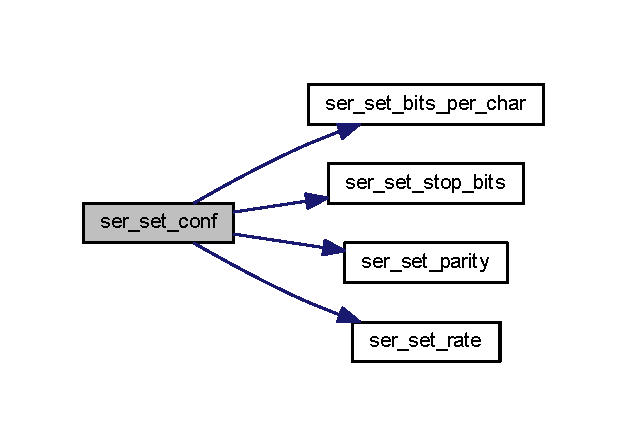
\includegraphics[width=301pt]{group__ser__port_ga1e0894432789b7311021c4f862335065_cgraph}
\end{center}
\end{figure}
\hypertarget{group__ser__port_ga4a963c8e3cfb978a4e4a026add12483f}{}\label{group__ser__port_ga4a963c8e3cfb978a4e4a026add12483f} 
\index{ser\+\_\+port@{ser\+\_\+port}!ser\+\_\+set\+\_\+parity@{ser\+\_\+set\+\_\+parity}}
\index{ser\+\_\+set\+\_\+parity@{ser\+\_\+set\+\_\+parity}!ser\+\_\+port@{ser\+\_\+port}}
\subsubsection{\texorpdfstring{ser\+\_\+set\+\_\+parity()}{ser\_set\_parity()}}
{\footnotesize\ttfamily int ser\+\_\+set\+\_\+parity (\begin{DoxyParamCaption}\item[{unsigned short}]{base\+\_\+addr,  }\item[{int}]{parity }\end{DoxyParamCaption})}



Sets the value of bits per character in the respective serial port. 


\begin{DoxyParams}{Parameters}
{\em base\+\_\+addr} & address of the serial port whose configuration we want to change\\
\hline
{\em parity} & parity that the serial port will be set to (its format is as specified above by the teacher)\\
\hline
\end{DoxyParams}
\begin{DoxyReturn}{Returns}
value 0 in case of success, 1 otherwise 
\end{DoxyReturn}
\hypertarget{group__ser__port_ga2b6153e7105a706ea7a331770150ac55}{}\label{group__ser__port_ga2b6153e7105a706ea7a331770150ac55} 
\index{ser\+\_\+port@{ser\+\_\+port}!ser\+\_\+set\+\_\+rate@{ser\+\_\+set\+\_\+rate}}
\index{ser\+\_\+set\+\_\+rate@{ser\+\_\+set\+\_\+rate}!ser\+\_\+port@{ser\+\_\+port}}
\subsubsection{\texorpdfstring{ser\+\_\+set\+\_\+rate()}{ser\_set\_rate()}}
{\footnotesize\ttfamily int ser\+\_\+set\+\_\+rate (\begin{DoxyParamCaption}\item[{unsigned short}]{base\+\_\+addr,  }\item[{int}]{rate }\end{DoxyParamCaption})}



Sets the value of bits per character in the respective serial port. 


\begin{DoxyParams}{Parameters}
{\em base\+\_\+addr} & address of the serial port whose configuration we want to change\\
\hline
{\em rate} & rate that the serial port will be set to\\
\hline
\end{DoxyParams}
\begin{DoxyReturn}{Returns}
value 0 in case of success, 1 otherwise 
\end{DoxyReturn}
\hypertarget{group__ser__port_ga7d67a8d80697182bb1afe90a65875c90}{}\label{group__ser__port_ga7d67a8d80697182bb1afe90a65875c90} 
\index{ser\+\_\+port@{ser\+\_\+port}!ser\+\_\+set\+\_\+stop\+\_\+bits@{ser\+\_\+set\+\_\+stop\+\_\+bits}}
\index{ser\+\_\+set\+\_\+stop\+\_\+bits@{ser\+\_\+set\+\_\+stop\+\_\+bits}!ser\+\_\+port@{ser\+\_\+port}}
\subsubsection{\texorpdfstring{ser\+\_\+set\+\_\+stop\+\_\+bits()}{ser\_set\_stop\_bits()}}
{\footnotesize\ttfamily int ser\+\_\+set\+\_\+stop\+\_\+bits (\begin{DoxyParamCaption}\item[{unsigned short}]{base\+\_\+addr,  }\item[{int}]{bits }\end{DoxyParamCaption})}



Sets the value of bits per character in the respective serial port. 


\begin{DoxyParams}{Parameters}
{\em base\+\_\+addr} & address of the serial port whose configuration we want to change\\
\hline
{\em bits} & number stop bits that the serial port will be set to\\
\hline
\end{DoxyParams}
\begin{DoxyReturn}{Returns}
value 0 in case of success, 1 otherwise 
\end{DoxyReturn}

\hypertarget{group__timer}{}\section{timer}
\label{group__timer}\index{timer@{timer}}
\subsection*{Functions}
\begin{DoxyCompactItemize}
\item 
void \hyperlink{group__timer_ga05c1893c9a1e24ff5d76b2958adb8851}{ignore\+\_\+interrupts} (unsigned char hook\+\_\+id)
\item 
int \hyperlink{group__timer_ga915070da84f7a3baa2e0fe634cb4bcd8}{timer\+\_\+subscribe\+\_\+int} ()
\begin{DoxyCompactList}\small\item\em subscribes a timer interruption \end{DoxyCompactList}\item 
int \hyperlink{group__timer_gab9eea51549744bca5c5c923b388bb4ee}{timer\+\_\+unsubscribe\+\_\+int} ()
\begin{DoxyCompactList}\small\item\em unsubscribes a timer interruption \end{DoxyCompactList}\item 
int \hyperlink{group__timer_gada4efbb5c88275795526fc45f0814aa3}{timer\+\_\+set\+\_\+square} (unsigned long timer, unsigned long freq)
\begin{DoxyCompactList}\small\item\em sets the timer frequency \end{DoxyCompactList}\item 
int \hyperlink{group__timer_ga8eb3357bc05265afc4bea5bbbb480a53}{timer\+\_\+get\+\_\+conf} (unsigned long timer, unsigned char $\ast$st)
\begin{DoxyCompactList}\small\item\em Reads the input timer configuration via read-\/back command. \end{DoxyCompactList}\end{DoxyCompactItemize}
\subsection*{Variables}
\begin{DoxyCompactItemize}
\item 
int \hyperlink{group__timer_ga96e6321e488d93a8134897510c435eb7}{timer\+\_\+hook\+\_\+id}
\begin{DoxyCompactList}\small\item\em hook for handling timer interruptions \end{DoxyCompactList}\end{DoxyCompactItemize}


\subsection{Detailed Description}
Functions related to the timer 

\subsection{Function Documentation}
\hypertarget{group__timer_ga05c1893c9a1e24ff5d76b2958adb8851}{}\label{group__timer_ga05c1893c9a1e24ff5d76b2958adb8851} 
\index{timer@{timer}!ignore\+\_\+interrupts@{ignore\+\_\+interrupts}}
\index{ignore\+\_\+interrupts@{ignore\+\_\+interrupts}!timer@{timer}}
\subsubsection{\texorpdfstring{ignore\+\_\+interrupts()}{ignore\_interrupts()}}
{\footnotesize\ttfamily void ignore\+\_\+interrupts (\begin{DoxyParamCaption}\item[{unsigned char}]{hook\+\_\+id }\end{DoxyParamCaption})}

\hypertarget{group__timer_ga8eb3357bc05265afc4bea5bbbb480a53}{}\label{group__timer_ga8eb3357bc05265afc4bea5bbbb480a53} 
\index{timer@{timer}!timer\+\_\+get\+\_\+conf@{timer\+\_\+get\+\_\+conf}}
\index{timer\+\_\+get\+\_\+conf@{timer\+\_\+get\+\_\+conf}!timer@{timer}}
\subsubsection{\texorpdfstring{timer\+\_\+get\+\_\+conf()}{timer\_get\_conf()}}
{\footnotesize\ttfamily int timer\+\_\+get\+\_\+conf (\begin{DoxyParamCaption}\item[{unsigned long}]{timer,  }\item[{unsigned char $\ast$}]{st }\end{DoxyParamCaption})}



Reads the input timer configuration via read-\/back command. 


\begin{DoxyParams}{Parameters}
{\em timer} & Timer whose config to read (Ranges from 0 to 2) \\
\hline
{\em st} & Address of memory position to be filled with the timer config \\
\hline
\end{DoxyParams}
\begin{DoxyReturn}{Returns}
Return 0 upon success and non-\/zero otherwise 
\end{DoxyReturn}
\hypertarget{group__timer_gada4efbb5c88275795526fc45f0814aa3}{}\label{group__timer_gada4efbb5c88275795526fc45f0814aa3} 
\index{timer@{timer}!timer\+\_\+set\+\_\+square@{timer\+\_\+set\+\_\+square}}
\index{timer\+\_\+set\+\_\+square@{timer\+\_\+set\+\_\+square}!timer@{timer}}
\subsubsection{\texorpdfstring{timer\+\_\+set\+\_\+square()}{timer\_set\_square()}}
{\footnotesize\ttfamily int timer\+\_\+set\+\_\+square (\begin{DoxyParamCaption}\item[{unsigned long}]{timer,  }\item[{unsigned long}]{freq }\end{DoxyParamCaption})}



sets the timer frequency 


\begin{DoxyParams}{Parameters}
{\em timer} & -\/$>$ timer \\
\hline
{\em freq} & -\/$>$ frequence \\
\hline
\end{DoxyParams}
\begin{DoxyReturn}{Returns}
1 in case of success, o otherwise 
\end{DoxyReturn}
Here is the call graph for this function\+:
% FIG 0
\hypertarget{group__timer_ga915070da84f7a3baa2e0fe634cb4bcd8}{}\label{group__timer_ga915070da84f7a3baa2e0fe634cb4bcd8} 
\index{timer@{timer}!timer\+\_\+subscribe\+\_\+int@{timer\+\_\+subscribe\+\_\+int}}
\index{timer\+\_\+subscribe\+\_\+int@{timer\+\_\+subscribe\+\_\+int}!timer@{timer}}
\subsubsection{\texorpdfstring{timer\+\_\+subscribe\+\_\+int()}{timer\_subscribe\_int()}}
{\footnotesize\ttfamily int timer\+\_\+subscribe\+\_\+int (\begin{DoxyParamCaption}{ }\end{DoxyParamCaption})}



subscribes a timer interruption 

\begin{DoxyReturn}{Returns}
Return 0 upon success and non-\/zero otherwise 
\end{DoxyReturn}
\hypertarget{group__timer_gab9eea51549744bca5c5c923b388bb4ee}{}\label{group__timer_gab9eea51549744bca5c5c923b388bb4ee} 
\index{timer@{timer}!timer\+\_\+unsubscribe\+\_\+int@{timer\+\_\+unsubscribe\+\_\+int}}
\index{timer\+\_\+unsubscribe\+\_\+int@{timer\+\_\+unsubscribe\+\_\+int}!timer@{timer}}
\subsubsection{\texorpdfstring{timer\+\_\+unsubscribe\+\_\+int()}{timer\_unsubscribe\_int()}}
{\footnotesize\ttfamily int timer\+\_\+unsubscribe\+\_\+int (\begin{DoxyParamCaption}{ }\end{DoxyParamCaption})}



unsubscribes a timer interruption 

\begin{DoxyReturn}{Returns}
Return 0 upon success and non-\/zero otherwise 
\end{DoxyReturn}


\subsection{Variable Documentation}
\hypertarget{group__timer_ga96e6321e488d93a8134897510c435eb7}{}\label{group__timer_ga96e6321e488d93a8134897510c435eb7} 
\index{timer@{timer}!timer\+\_\+hook\+\_\+id@{timer\+\_\+hook\+\_\+id}}
\index{timer\+\_\+hook\+\_\+id@{timer\+\_\+hook\+\_\+id}!timer@{timer}}
\subsubsection{\texorpdfstring{timer\+\_\+hook\+\_\+id}{timer\_hook\_id}}
{\footnotesize\ttfamily int timer\+\_\+hook\+\_\+id}



hook for handling timer interruptions 


\hypertarget{group__utilities}{}\section{utilities}
\label{group__utilities}\index{utilities@{utilities}}
\subsection*{Macros}
\begin{DoxyCompactItemize}
\item 
\#define \hyperlink{group__utilities_ga3a8ea58898cb58fc96013383d39f482c}{B\+IT}(n)~(0x01$<$$<$(n))
\item 
\#define \hyperlink{group__utilities_gab2e0399a4e6f9f5eb241bade77f59ea1}{I\+S\+\_\+\+B\+R\+E\+A\+K\+C\+O\+DE}(c)~(c$>$$>$7)
\item 
\#define \hyperlink{group__utilities_ga1a522aa19bcb695a9df30032a893bee3}{D\+E\+L\+A\+Y\+\_\+\+US}~20000
\end{DoxyCompactItemize}
\subsection*{Functions}
\begin{DoxyCompactItemize}
\item 
void \hyperlink{group__utilities_gaf3cb5100a651058103311c52a27b4105}{stringcpy} (char $\ast$dest, char $\ast$src)
\item 
void \hyperlink{group__utilities_ga971bb40926a0f370263e085d1e2ac690}{stringcat} (char $\ast$dest, char $\ast$src)
\item 
int \hyperlink{group__utilities_gaa662bd9797d0cdd2707c9ad14849be44}{hex\+\_\+to\+\_\+dec} (int x)
\begin{DoxyCompactList}\small\item\em converts a number from hexadecimal to decimal \end{DoxyCompactList}\item 
int \hyperlink{group__utilities_gafd4f329c8efb45c0dfff44525047a0fa}{abs} (int n)
\begin{DoxyCompactList}\small\item\em returns the absolute value of a number \end{DoxyCompactList}\item 
int \hyperlink{group__utilities_ga529fd7b4e2b2f87cec4a30c191673207}{floor2} (double x)
\begin{DoxyCompactList}\small\item\em returns the floor of a double \end{DoxyCompactList}\item 
int \hyperlink{group__utilities_ga35abf8e6bc22bc3736fbd65416d8c3a2}{round} (double x)
\begin{DoxyCompactList}\small\item\em rounds x to the closest integer for example (9.\+5-\/$>$10; 9.\+45-\/$>$9) \end{DoxyCompactList}\item 
int \hyperlink{group__utilities_ga67452a3b663c47b61edb379f159ae478}{sgn} (int n)
\begin{DoxyCompactList}\small\item\em returns sign of a number \end{DoxyCompactList}\item 
int \hyperlink{group__utilities_ga92a937ad6b303c03cc98f5fe9354d235}{samesign} (int x, int y)
\begin{DoxyCompactList}\small\item\em checks if two number have the same sign \end{DoxyCompactList}\item 
int \hyperlink{group__utilities_ga75e5e4e3c99b54b12f0bb43becded2d1}{samesignarray} (int size, int $\ast$arr)
\begin{DoxyCompactList}\small\item\em checks if all the elements of an array have the same sign \end{DoxyCompactList}\item 
char \hyperlink{group__utilities_gac0df2a1416cd59f12dbc6adfd5f69ba3}{two\+\_\+complement\+\_\+sym} (char c)
\begin{DoxyCompactList}\small\item\em returns the opposite number in two complement to c \end{DoxyCompactList}\item 
int \hyperlink{group__utilities_ga79537e8684629d74571e64c633bb5303}{conv\+\_\+to\+\_\+decimal} (char c)
\begin{DoxyCompactList}\small\item\em converts a char to decimal \end{DoxyCompactList}\end{DoxyCompactItemize}


\subsection{Detailed Description}
Simple functions that are used for conversions, comparisons, copies and solve math problems 

\subsection{Macro Definition Documentation}
\hypertarget{group__utilities_ga3a8ea58898cb58fc96013383d39f482c}{}\label{group__utilities_ga3a8ea58898cb58fc96013383d39f482c} 
\index{utilities@{utilities}!B\+IT@{B\+IT}}
\index{B\+IT@{B\+IT}!utilities@{utilities}}
\subsubsection{\texorpdfstring{B\+IT}{BIT}}
{\footnotesize\ttfamily \#define B\+IT(\begin{DoxyParamCaption}\item[{}]{n }\end{DoxyParamCaption})~(0x01$<$$<$(n))}

\hypertarget{group__utilities_ga1a522aa19bcb695a9df30032a893bee3}{}\label{group__utilities_ga1a522aa19bcb695a9df30032a893bee3} 
\index{utilities@{utilities}!D\+E\+L\+A\+Y\+\_\+\+US@{D\+E\+L\+A\+Y\+\_\+\+US}}
\index{D\+E\+L\+A\+Y\+\_\+\+US@{D\+E\+L\+A\+Y\+\_\+\+US}!utilities@{utilities}}
\subsubsection{\texorpdfstring{D\+E\+L\+A\+Y\+\_\+\+US}{DELAY\_US}}
{\footnotesize\ttfamily \#define D\+E\+L\+A\+Y\+\_\+\+US~20000}

\hypertarget{group__utilities_gab2e0399a4e6f9f5eb241bade77f59ea1}{}\label{group__utilities_gab2e0399a4e6f9f5eb241bade77f59ea1} 
\index{utilities@{utilities}!I\+S\+\_\+\+B\+R\+E\+A\+K\+C\+O\+DE@{I\+S\+\_\+\+B\+R\+E\+A\+K\+C\+O\+DE}}
\index{I\+S\+\_\+\+B\+R\+E\+A\+K\+C\+O\+DE@{I\+S\+\_\+\+B\+R\+E\+A\+K\+C\+O\+DE}!utilities@{utilities}}
\subsubsection{\texorpdfstring{I\+S\+\_\+\+B\+R\+E\+A\+K\+C\+O\+DE}{IS\_BREAKCODE}}
{\footnotesize\ttfamily \#define I\+S\+\_\+\+B\+R\+E\+A\+K\+C\+O\+DE(\begin{DoxyParamCaption}\item[{}]{c }\end{DoxyParamCaption})~(c$>$$>$7)}



\subsection{Function Documentation}
\hypertarget{group__utilities_gafd4f329c8efb45c0dfff44525047a0fa}{}\label{group__utilities_gafd4f329c8efb45c0dfff44525047a0fa} 
\index{utilities@{utilities}!abs@{abs}}
\index{abs@{abs}!utilities@{utilities}}
\subsubsection{\texorpdfstring{abs()}{abs()}}
{\footnotesize\ttfamily int abs (\begin{DoxyParamCaption}\item[{int}]{n }\end{DoxyParamCaption})}



returns the absolute value of a number 


\begin{DoxyParams}{Parameters}
{\em n} & number whose absolute value we want to know \\
\hline
\end{DoxyParams}
\begin{DoxyReturn}{Returns}
Absolute value of n 
\end{DoxyReturn}
\hypertarget{group__utilities_ga79537e8684629d74571e64c633bb5303}{}\label{group__utilities_ga79537e8684629d74571e64c633bb5303} 
\index{utilities@{utilities}!conv\+\_\+to\+\_\+decimal@{conv\+\_\+to\+\_\+decimal}}
\index{conv\+\_\+to\+\_\+decimal@{conv\+\_\+to\+\_\+decimal}!utilities@{utilities}}
\subsubsection{\texorpdfstring{conv\+\_\+to\+\_\+decimal()}{conv\_to\_decimal()}}
{\footnotesize\ttfamily int conv\+\_\+to\+\_\+decimal (\begin{DoxyParamCaption}\item[{char}]{c }\end{DoxyParamCaption})}



converts a char to decimal 


\begin{DoxyParams}{Parameters}
{\em c} & char to be converted to decimal \\
\hline
\end{DoxyParams}
\begin{DoxyReturn}{Returns}
Returns the conversion of c to decimal 
\end{DoxyReturn}
\hypertarget{group__utilities_ga529fd7b4e2b2f87cec4a30c191673207}{}\label{group__utilities_ga529fd7b4e2b2f87cec4a30c191673207} 
\index{utilities@{utilities}!floor2@{floor2}}
\index{floor2@{floor2}!utilities@{utilities}}
\subsubsection{\texorpdfstring{floor2()}{floor2()}}
{\footnotesize\ttfamily int floor2 (\begin{DoxyParamCaption}\item[{double}]{x }\end{DoxyParamCaption})}



returns the floor of a double 


\begin{DoxyParams}{Parameters}
{\em x} & double whose floor we want to know \\
\hline
\end{DoxyParams}
\begin{DoxyReturn}{Returns}
floor of x 
\end{DoxyReturn}
\hypertarget{group__utilities_gaa662bd9797d0cdd2707c9ad14849be44}{}\label{group__utilities_gaa662bd9797d0cdd2707c9ad14849be44} 
\index{utilities@{utilities}!hex\+\_\+to\+\_\+dec@{hex\+\_\+to\+\_\+dec}}
\index{hex\+\_\+to\+\_\+dec@{hex\+\_\+to\+\_\+dec}!utilities@{utilities}}
\subsubsection{\texorpdfstring{hex\+\_\+to\+\_\+dec()}{hex\_to\_dec()}}
{\footnotesize\ttfamily int hex\+\_\+to\+\_\+dec (\begin{DoxyParamCaption}\item[{int}]{x }\end{DoxyParamCaption})}



converts a number from hexadecimal to decimal 


\begin{DoxyParams}{Parameters}
{\em x} & number that is going to be converted \\
\hline
\end{DoxyParams}
\begin{DoxyReturn}{Returns}
number converted 
\end{DoxyReturn}
\hypertarget{group__utilities_ga35abf8e6bc22bc3736fbd65416d8c3a2}{}\label{group__utilities_ga35abf8e6bc22bc3736fbd65416d8c3a2} 
\index{utilities@{utilities}!round@{round}}
\index{round@{round}!utilities@{utilities}}
\subsubsection{\texorpdfstring{round()}{round()}}
{\footnotesize\ttfamily int round (\begin{DoxyParamCaption}\item[{double}]{x }\end{DoxyParamCaption})}



rounds x to the closest integer for example (9.\+5-\/$>$10; 9.\+45-\/$>$9) 


\begin{DoxyParams}{Parameters}
{\em x} & double whose closest integer we want to know \\
\hline
\end{DoxyParams}
\begin{DoxyReturn}{Returns}
closest integer to x 
\end{DoxyReturn}
Here is the call graph for this function\+:\nopagebreak
\begin{figure}[H]
\begin{center}
\leavevmode
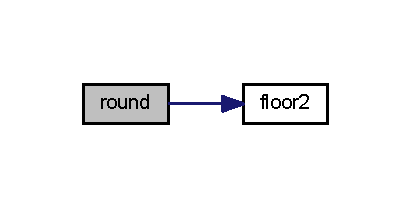
\includegraphics[width=197pt]{group__utilities_ga35abf8e6bc22bc3736fbd65416d8c3a2_cgraph}
\end{center}
\end{figure}
\hypertarget{group__utilities_ga92a937ad6b303c03cc98f5fe9354d235}{}\label{group__utilities_ga92a937ad6b303c03cc98f5fe9354d235} 
\index{utilities@{utilities}!samesign@{samesign}}
\index{samesign@{samesign}!utilities@{utilities}}
\subsubsection{\texorpdfstring{samesign()}{samesign()}}
{\footnotesize\ttfamily int samesign (\begin{DoxyParamCaption}\item[{int}]{x,  }\item[{int}]{y }\end{DoxyParamCaption})}



checks if two number have the same sign 


\begin{DoxyParams}{Parameters}
{\em x,y} & numbers whose signs we want to compare \\
\hline
\end{DoxyParams}
\begin{DoxyReturn}{Returns}
Returns 1 if both numbers have the same sign, 0 otherwise 
\end{DoxyReturn}
Here is the call graph for this function\+:\nopagebreak
\begin{figure}[H]
\begin{center}
\leavevmode
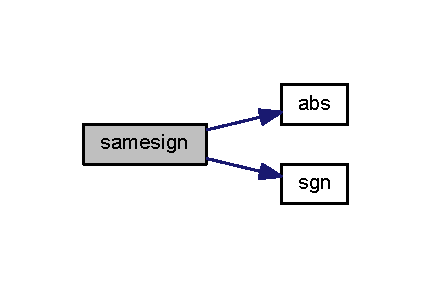
\includegraphics[width=207pt]{group__utilities_ga92a937ad6b303c03cc98f5fe9354d235_cgraph}
\end{center}
\end{figure}
\hypertarget{group__utilities_ga75e5e4e3c99b54b12f0bb43becded2d1}{}\label{group__utilities_ga75e5e4e3c99b54b12f0bb43becded2d1} 
\index{utilities@{utilities}!samesignarray@{samesignarray}}
\index{samesignarray@{samesignarray}!utilities@{utilities}}
\subsubsection{\texorpdfstring{samesignarray()}{samesignarray()}}
{\footnotesize\ttfamily int samesignarray (\begin{DoxyParamCaption}\item[{int}]{size,  }\item[{int $\ast$}]{arr }\end{DoxyParamCaption})}



checks if all the elements of an array have the same sign 


\begin{DoxyParams}{Parameters}
{\em size} & size of an array \\
\hline
\end{DoxyParams}
\begin{DoxyReturn}{Returns}
Returns 1 if all numbers have the same sign, 0 otherwise 
\end{DoxyReturn}
Here is the call graph for this function\+:\nopagebreak
\begin{figure}[H]
\begin{center}
\leavevmode
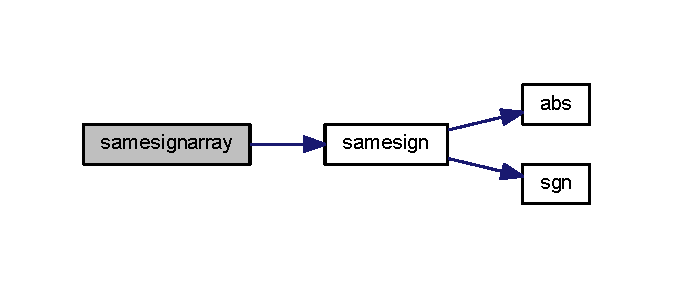
\includegraphics[width=323pt]{group__utilities_ga75e5e4e3c99b54b12f0bb43becded2d1_cgraph}
\end{center}
\end{figure}
\hypertarget{group__utilities_ga67452a3b663c47b61edb379f159ae478}{}\label{group__utilities_ga67452a3b663c47b61edb379f159ae478} 
\index{utilities@{utilities}!sgn@{sgn}}
\index{sgn@{sgn}!utilities@{utilities}}
\subsubsection{\texorpdfstring{sgn()}{sgn()}}
{\footnotesize\ttfamily int sgn (\begin{DoxyParamCaption}\item[{int}]{n }\end{DoxyParamCaption})}



returns sign of a number 


\begin{DoxyParams}{Parameters}
{\em n} & number whose sign we want to know \\
\hline
\end{DoxyParams}
\begin{DoxyReturn}{Returns}
sign of n 
\end{DoxyReturn}
\hypertarget{group__utilities_ga971bb40926a0f370263e085d1e2ac690}{}\label{group__utilities_ga971bb40926a0f370263e085d1e2ac690} 
\index{utilities@{utilities}!stringcat@{stringcat}}
\index{stringcat@{stringcat}!utilities@{utilities}}
\subsubsection{\texorpdfstring{stringcat()}{stringcat()}}
{\footnotesize\ttfamily void stringcat (\begin{DoxyParamCaption}\item[{char $\ast$}]{dest,  }\item[{char $\ast$}]{src }\end{DoxyParamCaption})}

\hypertarget{group__utilities_gaf3cb5100a651058103311c52a27b4105}{}\label{group__utilities_gaf3cb5100a651058103311c52a27b4105} 
\index{utilities@{utilities}!stringcpy@{stringcpy}}
\index{stringcpy@{stringcpy}!utilities@{utilities}}
\subsubsection{\texorpdfstring{stringcpy()}{stringcpy()}}
{\footnotesize\ttfamily void stringcpy (\begin{DoxyParamCaption}\item[{char $\ast$}]{dest,  }\item[{char $\ast$}]{src }\end{DoxyParamCaption})}

\hypertarget{group__utilities_gac0df2a1416cd59f12dbc6adfd5f69ba3}{}\label{group__utilities_gac0df2a1416cd59f12dbc6adfd5f69ba3} 
\index{utilities@{utilities}!two\+\_\+complement\+\_\+sym@{two\+\_\+complement\+\_\+sym}}
\index{two\+\_\+complement\+\_\+sym@{two\+\_\+complement\+\_\+sym}!utilities@{utilities}}
\subsubsection{\texorpdfstring{two\+\_\+complement\+\_\+sym()}{two\_complement\_sym()}}
{\footnotesize\ttfamily char two\+\_\+complement\+\_\+sym (\begin{DoxyParamCaption}\item[{char}]{c }\end{DoxyParamCaption})}



returns the opposite number in two complement to c 


\begin{DoxyParams}{Parameters}
{\em c} & value whose symetric in two complement we want to know \\
\hline
\end{DoxyParams}
\begin{DoxyReturn}{Returns}
the symetric in two\+\_\+complement for c 
\end{DoxyReturn}

\hypertarget{group__vbe}{}\section{vbe}
\label{group__vbe}\index{vbe@{vbe}}
\subsection*{Data Structures}
\begin{DoxyCompactItemize}
\item 
struct \hyperlink{structvbe__mode__info__t}{vbe\+\_\+mode\+\_\+info\+\_\+t}
\item 
struct \hyperlink{structvbe__info__block__t}{vbe\+\_\+info\+\_\+block\+\_\+t}
\end{DoxyCompactItemize}
\subsection*{Functions}
\begin{DoxyCompactItemize}
\item 
int \hyperlink{group__vbe_ga4ef3234e41f2050bc094a22049b69e45}{vbe\+\_\+get\+\_\+mode\+\_\+info} (unsigned short mode, \hyperlink{structvbe__mode__info__t}{vbe\+\_\+mode\+\_\+info\+\_\+t} $\ast$vmi\+\_\+p)
\begin{DoxyCompactList}\small\item\em Returns information on the input V\+BE mode, including screen dimensions, color depth and V\+R\+AM physical address. \end{DoxyCompactList}\item 
int \hyperlink{group__vbe_ga4e9da75c9063842b969ad400e5700c0c}{vbe\+\_\+get\+\_\+info\+\_\+block} (\hyperlink{structvbe__info__block__t}{vbe\+\_\+info\+\_\+block\+\_\+t} $\ast$vmi\+\_\+p)
\begin{DoxyCompactList}\small\item\em Returns information on the controller. \end{DoxyCompactList}\end{DoxyCompactItemize}
\subsection*{G\+E\+N\+E\+R\+IC M\+A\+C\+R\+OS}
\begin{DoxyCompactItemize}
\item 
\#define \hyperlink{group__vbe_ga68b87c2339cb305d66b69b5551b96c73}{P\+B2\+B\+A\+SE}(x)~(((x) $>$$>$ 4) \& 0x0\+F000)
\item 
\#define \hyperlink{group__vbe_ga70c65ed4c6d71865daa96d31befb33fd}{P\+B2\+O\+FF}(x)~((x) \& 0x0\+F\+F\+F\+F)
\item 
\#define \hyperlink{group__vbe_ga9cb0519a88e2860f94e49d7444ee5725}{V\+B\+E\+\_\+\+F\+U\+N\+C\+T\+I\+O\+N\+\_\+\+I\+N\+V\+O\+KE}~0x4F
\item 
\#define \hyperlink{group__vbe_ga13e1037464e7407d1df6aa4041b180cd}{V\+B\+E\+\_\+\+I\+N\+T\+E\+R\+R\+U\+PT}~0x10
\end{DoxyCompactItemize}
\subsection*{F\+U\+N\+C\+T\+I\+O\+NS}
\begin{DoxyCompactItemize}
\item 
\#define \hyperlink{group__vbe_ga7850c02defc99773b2704700c6cab3fd}{V\+B\+E\+\_\+\+R\+E\+T\+U\+R\+N\+\_\+\+C\+O\+N\+T\+R\+O\+L\+L\+ER}~0x00
\item 
\#define \hyperlink{group__vbe_gab9d80b9e6d7846ea3fa090c817771866}{V\+B\+E\+\_\+\+R\+E\+T\+U\+R\+N\+\_\+\+M\+O\+DE}~0x01
\item 
\#define \hyperlink{group__vbe_ga02477c4996ff058aee590b54f2146eb5}{V\+B\+E\+\_\+\+S\+E\+T\+\_\+\+M\+O\+DE}~0x02
\end{DoxyCompactItemize}
\subsection*{V\+BE R\+E\+T\+U\+RN S\+T\+A\+T\+US}
\begin{DoxyCompactItemize}
\item 
\#define \hyperlink{group__vbe_gaf48e8544d690af8d91d99653bad50a28}{V\+B\+E\+\_\+\+F\+U\+N\+C\+T\+I\+O\+N\+\_\+\+S\+U\+C\+C\+E\+SS}~0x00
\item 
\#define \hyperlink{group__vbe_ga0a4df98507b443e279641268d5583a3e}{V\+B\+E\+\_\+\+F\+U\+N\+C\+T\+I\+O\+N\+\_\+\+F\+A\+I\+L\+ED}~0x01
\item 
\#define \hyperlink{group__vbe_ga265850c04b2ec9164871c40cb8aa3b4f}{V\+B\+E\+\_\+\+F\+U\+N\+C\+T\+I\+O\+N\+\_\+\+N\+O\+T\+\_\+\+S\+U\+P\+P\+O\+R\+T\+ED}~0x02
\item 
\#define \hyperlink{group__vbe_ga48de88d26f563ed30a13e8158b90a54f}{V\+B\+E\+\_\+\+F\+U\+N\+C\+T\+I\+O\+N\+\_\+\+I\+N\+V\+A\+L\+ID}~0x03
\item 
\#define \hyperlink{group__vbe_ga4aba3d39cac7f9bc65f8b97a8daa88c6}{V\+B\+E\+\_\+\+F\+U\+N\+C\+T\+I\+O\+N\+\_\+\+S\+U\+P\+P\+O\+R\+T\+ED}~0x4F
\end{DoxyCompactItemize}
\subsection*{V\+BE M\+O\+D\+ES}
\begin{DoxyCompactItemize}
\item 
\#define \hyperlink{group__vbe_ga6d93a7fdde65a4c44c41cd0fae46a471}{V\+B\+E\+\_\+\+M\+O\+D\+E\+\_\+\+L\+I\+N\+E\+A\+R\+\_\+\+B\+IT}~14
\item 
\#define \hyperlink{group__vbe_gaa0cd0b74a86aa2dc9eb78017743d6f1a}{V\+B\+E\+\_\+\+G\+R\+A\+P\+H\+I\+C\+\_\+\+M\+O\+DE}~0x105
\item 
\#define \hyperlink{group__vbe_gac01942dc601c03d128c481824b1ae1d3}{V\+B\+E\+\_\+117\+\_\+\+M\+O\+DE}~0x117
\item 
\#define \hyperlink{group__vbe_gaf744f251b7e7d0acd6224997e46def7b}{V\+B\+E\+\_\+565\+\_\+\+M\+O\+DE}~0x11A
\end{DoxyCompactItemize}


\subsection{Detailed Description}
Functions related to the V\+BE standard 

\subsection{Macro Definition Documentation}
\hypertarget{group__vbe_ga68b87c2339cb305d66b69b5551b96c73}{}\label{group__vbe_ga68b87c2339cb305d66b69b5551b96c73} 
\index{vbe@{vbe}!P\+B2\+B\+A\+SE@{P\+B2\+B\+A\+SE}}
\index{P\+B2\+B\+A\+SE@{P\+B2\+B\+A\+SE}!vbe@{vbe}}
\subsubsection{\texorpdfstring{P\+B2\+B\+A\+SE}{PB2BASE}}
{\footnotesize\ttfamily \#define P\+B2\+B\+A\+SE(\begin{DoxyParamCaption}\item[{}]{x }\end{DoxyParamCaption})~(((x) $>$$>$ 4) \& 0x0\+F000)}

\hypertarget{group__vbe_ga70c65ed4c6d71865daa96d31befb33fd}{}\label{group__vbe_ga70c65ed4c6d71865daa96d31befb33fd} 
\index{vbe@{vbe}!P\+B2\+O\+FF@{P\+B2\+O\+FF}}
\index{P\+B2\+O\+FF@{P\+B2\+O\+FF}!vbe@{vbe}}
\subsubsection{\texorpdfstring{P\+B2\+O\+FF}{PB2OFF}}
{\footnotesize\ttfamily \#define P\+B2\+O\+FF(\begin{DoxyParamCaption}\item[{}]{x }\end{DoxyParamCaption})~((x) \& 0x0\+F\+F\+F\+F)}

\hypertarget{group__vbe_gac01942dc601c03d128c481824b1ae1d3}{}\label{group__vbe_gac01942dc601c03d128c481824b1ae1d3} 
\index{vbe@{vbe}!V\+B\+E\+\_\+117\+\_\+\+M\+O\+DE@{V\+B\+E\+\_\+117\+\_\+\+M\+O\+DE}}
\index{V\+B\+E\+\_\+117\+\_\+\+M\+O\+DE@{V\+B\+E\+\_\+117\+\_\+\+M\+O\+DE}!vbe@{vbe}}
\subsubsection{\texorpdfstring{V\+B\+E\+\_\+117\+\_\+\+M\+O\+DE}{VBE\_117\_MODE}}
{\footnotesize\ttfamily \#define V\+B\+E\+\_\+117\+\_\+\+M\+O\+DE~0x117}

\hypertarget{group__vbe_gaf744f251b7e7d0acd6224997e46def7b}{}\label{group__vbe_gaf744f251b7e7d0acd6224997e46def7b} 
\index{vbe@{vbe}!V\+B\+E\+\_\+565\+\_\+\+M\+O\+DE@{V\+B\+E\+\_\+565\+\_\+\+M\+O\+DE}}
\index{V\+B\+E\+\_\+565\+\_\+\+M\+O\+DE@{V\+B\+E\+\_\+565\+\_\+\+M\+O\+DE}!vbe@{vbe}}
\subsubsection{\texorpdfstring{V\+B\+E\+\_\+565\+\_\+\+M\+O\+DE}{VBE\_565\_MODE}}
{\footnotesize\ttfamily \#define V\+B\+E\+\_\+565\+\_\+\+M\+O\+DE~0x11A}

\hypertarget{group__vbe_ga0a4df98507b443e279641268d5583a3e}{}\label{group__vbe_ga0a4df98507b443e279641268d5583a3e} 
\index{vbe@{vbe}!V\+B\+E\+\_\+\+F\+U\+N\+C\+T\+I\+O\+N\+\_\+\+F\+A\+I\+L\+ED@{V\+B\+E\+\_\+\+F\+U\+N\+C\+T\+I\+O\+N\+\_\+\+F\+A\+I\+L\+ED}}
\index{V\+B\+E\+\_\+\+F\+U\+N\+C\+T\+I\+O\+N\+\_\+\+F\+A\+I\+L\+ED@{V\+B\+E\+\_\+\+F\+U\+N\+C\+T\+I\+O\+N\+\_\+\+F\+A\+I\+L\+ED}!vbe@{vbe}}
\subsubsection{\texorpdfstring{V\+B\+E\+\_\+\+F\+U\+N\+C\+T\+I\+O\+N\+\_\+\+F\+A\+I\+L\+ED}{VBE\_FUNCTION\_FAILED}}
{\footnotesize\ttfamily \#define V\+B\+E\+\_\+\+F\+U\+N\+C\+T\+I\+O\+N\+\_\+\+F\+A\+I\+L\+ED~0x01}

\hypertarget{group__vbe_ga48de88d26f563ed30a13e8158b90a54f}{}\label{group__vbe_ga48de88d26f563ed30a13e8158b90a54f} 
\index{vbe@{vbe}!V\+B\+E\+\_\+\+F\+U\+N\+C\+T\+I\+O\+N\+\_\+\+I\+N\+V\+A\+L\+ID@{V\+B\+E\+\_\+\+F\+U\+N\+C\+T\+I\+O\+N\+\_\+\+I\+N\+V\+A\+L\+ID}}
\index{V\+B\+E\+\_\+\+F\+U\+N\+C\+T\+I\+O\+N\+\_\+\+I\+N\+V\+A\+L\+ID@{V\+B\+E\+\_\+\+F\+U\+N\+C\+T\+I\+O\+N\+\_\+\+I\+N\+V\+A\+L\+ID}!vbe@{vbe}}
\subsubsection{\texorpdfstring{V\+B\+E\+\_\+\+F\+U\+N\+C\+T\+I\+O\+N\+\_\+\+I\+N\+V\+A\+L\+ID}{VBE\_FUNCTION\_INVALID}}
{\footnotesize\ttfamily \#define V\+B\+E\+\_\+\+F\+U\+N\+C\+T\+I\+O\+N\+\_\+\+I\+N\+V\+A\+L\+ID~0x03}

\hypertarget{group__vbe_ga9cb0519a88e2860f94e49d7444ee5725}{}\label{group__vbe_ga9cb0519a88e2860f94e49d7444ee5725} 
\index{vbe@{vbe}!V\+B\+E\+\_\+\+F\+U\+N\+C\+T\+I\+O\+N\+\_\+\+I\+N\+V\+O\+KE@{V\+B\+E\+\_\+\+F\+U\+N\+C\+T\+I\+O\+N\+\_\+\+I\+N\+V\+O\+KE}}
\index{V\+B\+E\+\_\+\+F\+U\+N\+C\+T\+I\+O\+N\+\_\+\+I\+N\+V\+O\+KE@{V\+B\+E\+\_\+\+F\+U\+N\+C\+T\+I\+O\+N\+\_\+\+I\+N\+V\+O\+KE}!vbe@{vbe}}
\subsubsection{\texorpdfstring{V\+B\+E\+\_\+\+F\+U\+N\+C\+T\+I\+O\+N\+\_\+\+I\+N\+V\+O\+KE}{VBE\_FUNCTION\_INVOKE}}
{\footnotesize\ttfamily \#define V\+B\+E\+\_\+\+F\+U\+N\+C\+T\+I\+O\+N\+\_\+\+I\+N\+V\+O\+KE~0x4F}

\hypertarget{group__vbe_ga265850c04b2ec9164871c40cb8aa3b4f}{}\label{group__vbe_ga265850c04b2ec9164871c40cb8aa3b4f} 
\index{vbe@{vbe}!V\+B\+E\+\_\+\+F\+U\+N\+C\+T\+I\+O\+N\+\_\+\+N\+O\+T\+\_\+\+S\+U\+P\+P\+O\+R\+T\+ED@{V\+B\+E\+\_\+\+F\+U\+N\+C\+T\+I\+O\+N\+\_\+\+N\+O\+T\+\_\+\+S\+U\+P\+P\+O\+R\+T\+ED}}
\index{V\+B\+E\+\_\+\+F\+U\+N\+C\+T\+I\+O\+N\+\_\+\+N\+O\+T\+\_\+\+S\+U\+P\+P\+O\+R\+T\+ED@{V\+B\+E\+\_\+\+F\+U\+N\+C\+T\+I\+O\+N\+\_\+\+N\+O\+T\+\_\+\+S\+U\+P\+P\+O\+R\+T\+ED}!vbe@{vbe}}
\subsubsection{\texorpdfstring{V\+B\+E\+\_\+\+F\+U\+N\+C\+T\+I\+O\+N\+\_\+\+N\+O\+T\+\_\+\+S\+U\+P\+P\+O\+R\+T\+ED}{VBE\_FUNCTION\_NOT\_SUPPORTED}}
{\footnotesize\ttfamily \#define V\+B\+E\+\_\+\+F\+U\+N\+C\+T\+I\+O\+N\+\_\+\+N\+O\+T\+\_\+\+S\+U\+P\+P\+O\+R\+T\+ED~0x02}

\hypertarget{group__vbe_gaf48e8544d690af8d91d99653bad50a28}{}\label{group__vbe_gaf48e8544d690af8d91d99653bad50a28} 
\index{vbe@{vbe}!V\+B\+E\+\_\+\+F\+U\+N\+C\+T\+I\+O\+N\+\_\+\+S\+U\+C\+C\+E\+SS@{V\+B\+E\+\_\+\+F\+U\+N\+C\+T\+I\+O\+N\+\_\+\+S\+U\+C\+C\+E\+SS}}
\index{V\+B\+E\+\_\+\+F\+U\+N\+C\+T\+I\+O\+N\+\_\+\+S\+U\+C\+C\+E\+SS@{V\+B\+E\+\_\+\+F\+U\+N\+C\+T\+I\+O\+N\+\_\+\+S\+U\+C\+C\+E\+SS}!vbe@{vbe}}
\subsubsection{\texorpdfstring{V\+B\+E\+\_\+\+F\+U\+N\+C\+T\+I\+O\+N\+\_\+\+S\+U\+C\+C\+E\+SS}{VBE\_FUNCTION\_SUCCESS}}
{\footnotesize\ttfamily \#define V\+B\+E\+\_\+\+F\+U\+N\+C\+T\+I\+O\+N\+\_\+\+S\+U\+C\+C\+E\+SS~0x00}

\hypertarget{group__vbe_ga4aba3d39cac7f9bc65f8b97a8daa88c6}{}\label{group__vbe_ga4aba3d39cac7f9bc65f8b97a8daa88c6} 
\index{vbe@{vbe}!V\+B\+E\+\_\+\+F\+U\+N\+C\+T\+I\+O\+N\+\_\+\+S\+U\+P\+P\+O\+R\+T\+ED@{V\+B\+E\+\_\+\+F\+U\+N\+C\+T\+I\+O\+N\+\_\+\+S\+U\+P\+P\+O\+R\+T\+ED}}
\index{V\+B\+E\+\_\+\+F\+U\+N\+C\+T\+I\+O\+N\+\_\+\+S\+U\+P\+P\+O\+R\+T\+ED@{V\+B\+E\+\_\+\+F\+U\+N\+C\+T\+I\+O\+N\+\_\+\+S\+U\+P\+P\+O\+R\+T\+ED}!vbe@{vbe}}
\subsubsection{\texorpdfstring{V\+B\+E\+\_\+\+F\+U\+N\+C\+T\+I\+O\+N\+\_\+\+S\+U\+P\+P\+O\+R\+T\+ED}{VBE\_FUNCTION\_SUPPORTED}}
{\footnotesize\ttfamily \#define V\+B\+E\+\_\+\+F\+U\+N\+C\+T\+I\+O\+N\+\_\+\+S\+U\+P\+P\+O\+R\+T\+ED~0x4F}

\hypertarget{group__vbe_gaa0cd0b74a86aa2dc9eb78017743d6f1a}{}\label{group__vbe_gaa0cd0b74a86aa2dc9eb78017743d6f1a} 
\index{vbe@{vbe}!V\+B\+E\+\_\+\+G\+R\+A\+P\+H\+I\+C\+\_\+\+M\+O\+DE@{V\+B\+E\+\_\+\+G\+R\+A\+P\+H\+I\+C\+\_\+\+M\+O\+DE}}
\index{V\+B\+E\+\_\+\+G\+R\+A\+P\+H\+I\+C\+\_\+\+M\+O\+DE@{V\+B\+E\+\_\+\+G\+R\+A\+P\+H\+I\+C\+\_\+\+M\+O\+DE}!vbe@{vbe}}
\subsubsection{\texorpdfstring{V\+B\+E\+\_\+\+G\+R\+A\+P\+H\+I\+C\+\_\+\+M\+O\+DE}{VBE\_GRAPHIC\_MODE}}
{\footnotesize\ttfamily \#define V\+B\+E\+\_\+\+G\+R\+A\+P\+H\+I\+C\+\_\+\+M\+O\+DE~0x105}

\hypertarget{group__vbe_ga13e1037464e7407d1df6aa4041b180cd}{}\label{group__vbe_ga13e1037464e7407d1df6aa4041b180cd} 
\index{vbe@{vbe}!V\+B\+E\+\_\+\+I\+N\+T\+E\+R\+R\+U\+PT@{V\+B\+E\+\_\+\+I\+N\+T\+E\+R\+R\+U\+PT}}
\index{V\+B\+E\+\_\+\+I\+N\+T\+E\+R\+R\+U\+PT@{V\+B\+E\+\_\+\+I\+N\+T\+E\+R\+R\+U\+PT}!vbe@{vbe}}
\subsubsection{\texorpdfstring{V\+B\+E\+\_\+\+I\+N\+T\+E\+R\+R\+U\+PT}{VBE\_INTERRUPT}}
{\footnotesize\ttfamily \#define V\+B\+E\+\_\+\+I\+N\+T\+E\+R\+R\+U\+PT~0x10}

\hypertarget{group__vbe_ga6d93a7fdde65a4c44c41cd0fae46a471}{}\label{group__vbe_ga6d93a7fdde65a4c44c41cd0fae46a471} 
\index{vbe@{vbe}!V\+B\+E\+\_\+\+M\+O\+D\+E\+\_\+\+L\+I\+N\+E\+A\+R\+\_\+\+B\+IT@{V\+B\+E\+\_\+\+M\+O\+D\+E\+\_\+\+L\+I\+N\+E\+A\+R\+\_\+\+B\+IT}}
\index{V\+B\+E\+\_\+\+M\+O\+D\+E\+\_\+\+L\+I\+N\+E\+A\+R\+\_\+\+B\+IT@{V\+B\+E\+\_\+\+M\+O\+D\+E\+\_\+\+L\+I\+N\+E\+A\+R\+\_\+\+B\+IT}!vbe@{vbe}}
\subsubsection{\texorpdfstring{V\+B\+E\+\_\+\+M\+O\+D\+E\+\_\+\+L\+I\+N\+E\+A\+R\+\_\+\+B\+IT}{VBE\_MODE\_LINEAR\_BIT}}
{\footnotesize\ttfamily \#define V\+B\+E\+\_\+\+M\+O\+D\+E\+\_\+\+L\+I\+N\+E\+A\+R\+\_\+\+B\+IT~14}

\hypertarget{group__vbe_ga7850c02defc99773b2704700c6cab3fd}{}\label{group__vbe_ga7850c02defc99773b2704700c6cab3fd} 
\index{vbe@{vbe}!V\+B\+E\+\_\+\+R\+E\+T\+U\+R\+N\+\_\+\+C\+O\+N\+T\+R\+O\+L\+L\+ER@{V\+B\+E\+\_\+\+R\+E\+T\+U\+R\+N\+\_\+\+C\+O\+N\+T\+R\+O\+L\+L\+ER}}
\index{V\+B\+E\+\_\+\+R\+E\+T\+U\+R\+N\+\_\+\+C\+O\+N\+T\+R\+O\+L\+L\+ER@{V\+B\+E\+\_\+\+R\+E\+T\+U\+R\+N\+\_\+\+C\+O\+N\+T\+R\+O\+L\+L\+ER}!vbe@{vbe}}
\subsubsection{\texorpdfstring{V\+B\+E\+\_\+\+R\+E\+T\+U\+R\+N\+\_\+\+C\+O\+N\+T\+R\+O\+L\+L\+ER}{VBE\_RETURN\_CONTROLLER}}
{\footnotesize\ttfamily \#define V\+B\+E\+\_\+\+R\+E\+T\+U\+R\+N\+\_\+\+C\+O\+N\+T\+R\+O\+L\+L\+ER~0x00}

\hypertarget{group__vbe_gab9d80b9e6d7846ea3fa090c817771866}{}\label{group__vbe_gab9d80b9e6d7846ea3fa090c817771866} 
\index{vbe@{vbe}!V\+B\+E\+\_\+\+R\+E\+T\+U\+R\+N\+\_\+\+M\+O\+DE@{V\+B\+E\+\_\+\+R\+E\+T\+U\+R\+N\+\_\+\+M\+O\+DE}}
\index{V\+B\+E\+\_\+\+R\+E\+T\+U\+R\+N\+\_\+\+M\+O\+DE@{V\+B\+E\+\_\+\+R\+E\+T\+U\+R\+N\+\_\+\+M\+O\+DE}!vbe@{vbe}}
\subsubsection{\texorpdfstring{V\+B\+E\+\_\+\+R\+E\+T\+U\+R\+N\+\_\+\+M\+O\+DE}{VBE\_RETURN\_MODE}}
{\footnotesize\ttfamily \#define V\+B\+E\+\_\+\+R\+E\+T\+U\+R\+N\+\_\+\+M\+O\+DE~0x01}

\hypertarget{group__vbe_ga02477c4996ff058aee590b54f2146eb5}{}\label{group__vbe_ga02477c4996ff058aee590b54f2146eb5} 
\index{vbe@{vbe}!V\+B\+E\+\_\+\+S\+E\+T\+\_\+\+M\+O\+DE@{V\+B\+E\+\_\+\+S\+E\+T\+\_\+\+M\+O\+DE}}
\index{V\+B\+E\+\_\+\+S\+E\+T\+\_\+\+M\+O\+DE@{V\+B\+E\+\_\+\+S\+E\+T\+\_\+\+M\+O\+DE}!vbe@{vbe}}
\subsubsection{\texorpdfstring{V\+B\+E\+\_\+\+S\+E\+T\+\_\+\+M\+O\+DE}{VBE\_SET\_MODE}}
{\footnotesize\ttfamily \#define V\+B\+E\+\_\+\+S\+E\+T\+\_\+\+M\+O\+DE~0x02}



\subsection{Function Documentation}
\hypertarget{group__vbe_ga4e9da75c9063842b969ad400e5700c0c}{}\label{group__vbe_ga4e9da75c9063842b969ad400e5700c0c} 
\index{vbe@{vbe}!vbe\+\_\+get\+\_\+info\+\_\+block@{vbe\+\_\+get\+\_\+info\+\_\+block}}
\index{vbe\+\_\+get\+\_\+info\+\_\+block@{vbe\+\_\+get\+\_\+info\+\_\+block}!vbe@{vbe}}
\subsubsection{\texorpdfstring{vbe\+\_\+get\+\_\+info\+\_\+block()}{vbe\_get\_info\_block()}}
{\footnotesize\ttfamily int vbe\+\_\+get\+\_\+info\+\_\+block (\begin{DoxyParamCaption}\item[{\hyperlink{structvbe__info__block__t}{vbe\+\_\+info\+\_\+block\+\_\+t} $\ast$}]{vmi\+\_\+p }\end{DoxyParamCaption})}



Returns information on the controller. 


\begin{DoxyParams}{Parameters}
{\em vmi\+\_\+p} & variable where the controller information should be stored\\
\hline
\end{DoxyParams}
\begin{DoxyReturn}{Returns}
0 on success, non-\/zero otherwise 
\end{DoxyReturn}
Here is the call graph for this function\+:
% FIG 0
\hypertarget{group__vbe_ga4ef3234e41f2050bc094a22049b69e45}{}\label{group__vbe_ga4ef3234e41f2050bc094a22049b69e45} 
\index{vbe@{vbe}!vbe\+\_\+get\+\_\+mode\+\_\+info@{vbe\+\_\+get\+\_\+mode\+\_\+info}}
\index{vbe\+\_\+get\+\_\+mode\+\_\+info@{vbe\+\_\+get\+\_\+mode\+\_\+info}!vbe@{vbe}}
\subsubsection{\texorpdfstring{vbe\+\_\+get\+\_\+mode\+\_\+info()}{vbe\_get\_mode\_info()}}
{\footnotesize\ttfamily int vbe\+\_\+get\+\_\+mode\+\_\+info (\begin{DoxyParamCaption}\item[{unsigned short}]{mode,  }\item[{\hyperlink{structvbe__mode__info__t}{vbe\+\_\+mode\+\_\+info\+\_\+t} $\ast$}]{vmi\+\_\+p }\end{DoxyParamCaption})}



Returns information on the input V\+BE mode, including screen dimensions, color depth and V\+R\+AM physical address. 

Initializes unpacked vbe\+\_\+mode\+\_\+\+\_\+info\+\_\+t structure passed as an address with the information of the input mode, by calling V\+BE function 0x01 Return V\+BE Mode Information and unpacking the Mode\+Info\+Block struct returned by that function.


\begin{DoxyParams}{Parameters}
{\em mode} & mode whose information should be returned \\
\hline
{\em vmi\+\_\+p} & address of \hyperlink{structvbe__mode__info__t}{vbe\+\_\+mode\+\_\+info\+\_\+t} structure to be initialized \\
\hline
\end{DoxyParams}
\begin{DoxyReturn}{Returns}
0 on success, non-\/zero otherwise 
\end{DoxyReturn}
Here is the call graph for this function\+:
% FIG 1

\hypertarget{group__video__gr}{}\section{video\+\_\+gr}
\label{group__video__gr}\index{video\+\_\+gr@{video\+\_\+gr}}
\subsection*{Functions}
\begin{DoxyCompactItemize}
\item 
unsigned \hyperlink{group__video__gr_ga80f6be1470280496d613f43fbf4f576c}{get\+Mouse\+\_\+buffer} ()
\begin{DoxyCompactList}\small\item\em gets pointer to variable mouse\+\_\+buffer \end{DoxyCompactList}\item 
unsigned \hyperlink{group__video__gr_gafa0e51016d7aa337778300ba2ec70a74}{get\+Double\+\_\+buffer} ()
\begin{DoxyCompactList}\small\item\em gets pointer to variable double\+\_\+buffer \end{DoxyCompactList}\item 
unsigned \hyperlink{group__video__gr_gae633b6fb3ed1e90fdcbc7b4c65ffe2ef}{get\+Video\+\_\+\+\_\+mem} ()
\begin{DoxyCompactList}\small\item\em gets pointer to variable video\+\_\+mem \end{DoxyCompactList}\item 
unsigned \hyperlink{group__video__gr_gaf597a67a797839097222fa9b4ae20b3f}{get\+H\+\_\+res} ()
\begin{DoxyCompactList}\small\item\em gets horizontal resolution of the screen \end{DoxyCompactList}\item 
unsigned \hyperlink{group__video__gr_ga36f1c43e43d903e085207548cf8d48a2}{get\+V\+\_\+res} ()
\begin{DoxyCompactList}\small\item\em gets vertical resolution of the screen \end{DoxyCompactList}\item 
void $\ast$ \hyperlink{group__video__gr_gacef21667c79365d57a084bed994c2189}{vg\+\_\+init} (unsigned short mode)
\begin{DoxyCompactList}\small\item\em Initializes the video module in graphics mode. \end{DoxyCompactList}\item 
int \hyperlink{group__video__gr_ga42f593e6656f1a978315aff02b1bcebf}{vg\+\_\+exit} (void)
\begin{DoxyCompactList}\small\item\em Returns to default Minix 3 text mode (0x03\+: 25 x 80, 16 colors) \end{DoxyCompactList}\item 
int \hyperlink{group__video__gr_ga729c07175ab64956c7fd9944d7676888}{vg\+\_\+set\+\_\+pixel} (int x, int y, unsigned int color)
\begin{DoxyCompactList}\small\item\em sets the color of a pixel in the double buffer and in the mouse buffer \end{DoxyCompactList}\item 
int \hyperlink{group__video__gr_ga78765c3e4634b79d0c27b464be410803}{vg\+\_\+set\+\_\+mouse\+\_\+pixel} (int x, int y, unsigned int color)
\begin{DoxyCompactList}\small\item\em sets the color of a pixel in the mouse buffer \end{DoxyCompactList}\item 
int \hyperlink{group__video__gr_gafcdcee0785e2e5a0d0f1f460bf436403}{vg\+\_\+draw\+\_\+square} (int xi, int yi, int size, int color)
\begin{DoxyCompactList}\small\item\em draws a square in the double buffer and in the mouse buffer \end{DoxyCompactList}\item 
int \hyperlink{group__video__gr_ga0410a09b926582249fb7c0a795c9d4fe}{vg\+\_\+draw\+\_\+circle} (int xi, int yi, int radius, int color)
\begin{DoxyCompactList}\small\item\em draws a circle in the double buffer and in the mouse buffer \end{DoxyCompactList}\item 
int \hyperlink{group__video__gr_gae50eb47e283e71498d323e815411acc3}{swap\+\_\+double\+\_\+video} ()
\begin{DoxyCompactList}\small\item\em copies the double\+\_\+buffer into the video\+\_\+buffer \end{DoxyCompactList}\item 
int \hyperlink{group__video__gr_ga8761e145d6f2249e0a4177ed7ff24299}{swap\+\_\+mouse\+\_\+video} ()
\begin{DoxyCompactList}\small\item\em copies the mouse\+\_\+buffer into the video\+\_\+buffer \end{DoxyCompactList}\item 
int \hyperlink{group__video__gr_ga56155e15f2cbeb0c0790c3b22db43a78}{swap\+\_\+mouse\+\_\+double} ()
\begin{DoxyCompactList}\small\item\em copies the mouse\+\_\+buffer into the double\+\_\+buffer \end{DoxyCompactList}\item 
int \hyperlink{group__video__gr_gacbc2b21e05ad693bb6ed614f87329f05}{swap\+\_\+double\+\_\+mouse} ()
\begin{DoxyCompactList}\small\item\em copies the double\+\_\+buffer into the mouse\+\_\+buffer \end{DoxyCompactList}\item 
int \hyperlink{group__video__gr_gaeae89e446fefdba5e72413ff38727f44}{mouse\+\_\+to\+\_\+double} (int x, int y)
\begin{DoxyCompactList}\small\item\em sets a pixel in the mouse buffer to the color of the corresponding pixel in the double buffer \end{DoxyCompactList}\end{DoxyCompactItemize}


\subsection{Detailed Description}
Functions for outputing data to screen in graphics mode 

\subsection{Function Documentation}
\hypertarget{group__video__gr_gafa0e51016d7aa337778300ba2ec70a74}{}\label{group__video__gr_gafa0e51016d7aa337778300ba2ec70a74} 
\index{video\+\_\+gr@{video\+\_\+gr}!get\+Double\+\_\+buffer@{get\+Double\+\_\+buffer}}
\index{get\+Double\+\_\+buffer@{get\+Double\+\_\+buffer}!video\+\_\+gr@{video\+\_\+gr}}
\subsubsection{\texorpdfstring{get\+Double\+\_\+buffer()}{getDouble\_buffer()}}
{\footnotesize\ttfamily unsigned get\+Double\+\_\+buffer (\begin{DoxyParamCaption}{ }\end{DoxyParamCaption})}



gets pointer to variable double\+\_\+buffer 

\begin{DoxyReturn}{Returns}
pointer to variable double\+\_\+buffer 
\end{DoxyReturn}
\hypertarget{group__video__gr_gaf597a67a797839097222fa9b4ae20b3f}{}\label{group__video__gr_gaf597a67a797839097222fa9b4ae20b3f} 
\index{video\+\_\+gr@{video\+\_\+gr}!get\+H\+\_\+res@{get\+H\+\_\+res}}
\index{get\+H\+\_\+res@{get\+H\+\_\+res}!video\+\_\+gr@{video\+\_\+gr}}
\subsubsection{\texorpdfstring{get\+H\+\_\+res()}{getH\_res()}}
{\footnotesize\ttfamily unsigned get\+H\+\_\+res (\begin{DoxyParamCaption}{ }\end{DoxyParamCaption})}



gets horizontal resolution of the screen 

\begin{DoxyReturn}{Returns}
horizontal resolution 
\end{DoxyReturn}
\hypertarget{group__video__gr_ga80f6be1470280496d613f43fbf4f576c}{}\label{group__video__gr_ga80f6be1470280496d613f43fbf4f576c} 
\index{video\+\_\+gr@{video\+\_\+gr}!get\+Mouse\+\_\+buffer@{get\+Mouse\+\_\+buffer}}
\index{get\+Mouse\+\_\+buffer@{get\+Mouse\+\_\+buffer}!video\+\_\+gr@{video\+\_\+gr}}
\subsubsection{\texorpdfstring{get\+Mouse\+\_\+buffer()}{getMouse\_buffer()}}
{\footnotesize\ttfamily unsigned get\+Mouse\+\_\+buffer (\begin{DoxyParamCaption}{ }\end{DoxyParamCaption})}



gets pointer to variable mouse\+\_\+buffer 

\begin{DoxyReturn}{Returns}
pointer to variable mouse\+\_\+buffer 
\end{DoxyReturn}
\hypertarget{group__video__gr_ga36f1c43e43d903e085207548cf8d48a2}{}\label{group__video__gr_ga36f1c43e43d903e085207548cf8d48a2} 
\index{video\+\_\+gr@{video\+\_\+gr}!get\+V\+\_\+res@{get\+V\+\_\+res}}
\index{get\+V\+\_\+res@{get\+V\+\_\+res}!video\+\_\+gr@{video\+\_\+gr}}
\subsubsection{\texorpdfstring{get\+V\+\_\+res()}{getV\_res()}}
{\footnotesize\ttfamily unsigned get\+V\+\_\+res (\begin{DoxyParamCaption}{ }\end{DoxyParamCaption})}



gets vertical resolution of the screen 

\begin{DoxyReturn}{Returns}
vertical resolution 
\end{DoxyReturn}
\hypertarget{group__video__gr_gae633b6fb3ed1e90fdcbc7b4c65ffe2ef}{}\label{group__video__gr_gae633b6fb3ed1e90fdcbc7b4c65ffe2ef} 
\index{video\+\_\+gr@{video\+\_\+gr}!get\+Video\+\_\+\+\_\+mem@{get\+Video\+\_\+\+\_\+mem}}
\index{get\+Video\+\_\+\+\_\+mem@{get\+Video\+\_\+\+\_\+mem}!video\+\_\+gr@{video\+\_\+gr}}
\subsubsection{\texorpdfstring{get\+Video\+\_\+\+\_\+mem()}{getVideo\_\_mem()}}
{\footnotesize\ttfamily unsigned get\+Video\+\_\+\+\_\+mem (\begin{DoxyParamCaption}{ }\end{DoxyParamCaption})}



gets pointer to variable video\+\_\+mem 

\begin{DoxyReturn}{Returns}
pointer to variable video\+\_\+mem 
\end{DoxyReturn}
\hypertarget{group__video__gr_gaeae89e446fefdba5e72413ff38727f44}{}\label{group__video__gr_gaeae89e446fefdba5e72413ff38727f44} 
\index{video\+\_\+gr@{video\+\_\+gr}!mouse\+\_\+to\+\_\+double@{mouse\+\_\+to\+\_\+double}}
\index{mouse\+\_\+to\+\_\+double@{mouse\+\_\+to\+\_\+double}!video\+\_\+gr@{video\+\_\+gr}}
\subsubsection{\texorpdfstring{mouse\+\_\+to\+\_\+double()}{mouse\_to\_double()}}
{\footnotesize\ttfamily int mouse\+\_\+to\+\_\+double (\begin{DoxyParamCaption}\item[{int}]{x,  }\item[{int}]{y }\end{DoxyParamCaption})}



sets a pixel in the mouse buffer to the color of the corresponding pixel in the double buffer 


\begin{DoxyParams}{Parameters}
{\em x,y} & coordinates of the pixel \\
\hline
\end{DoxyParams}
\begin{DoxyReturn}{Returns}
0 in case of success, 1 otherwise 
\end{DoxyReturn}
\hypertarget{group__video__gr_gacbc2b21e05ad693bb6ed614f87329f05}{}\label{group__video__gr_gacbc2b21e05ad693bb6ed614f87329f05} 
\index{video\+\_\+gr@{video\+\_\+gr}!swap\+\_\+double\+\_\+mouse@{swap\+\_\+double\+\_\+mouse}}
\index{swap\+\_\+double\+\_\+mouse@{swap\+\_\+double\+\_\+mouse}!video\+\_\+gr@{video\+\_\+gr}}
\subsubsection{\texorpdfstring{swap\+\_\+double\+\_\+mouse()}{swap\_double\_mouse()}}
{\footnotesize\ttfamily int swap\+\_\+double\+\_\+mouse (\begin{DoxyParamCaption}{ }\end{DoxyParamCaption})}



copies the double\+\_\+buffer into the mouse\+\_\+buffer 

\begin{DoxyReturn}{Returns}
0 in case of success, 1 otherwise 
\end{DoxyReturn}
\hypertarget{group__video__gr_gae50eb47e283e71498d323e815411acc3}{}\label{group__video__gr_gae50eb47e283e71498d323e815411acc3} 
\index{video\+\_\+gr@{video\+\_\+gr}!swap\+\_\+double\+\_\+video@{swap\+\_\+double\+\_\+video}}
\index{swap\+\_\+double\+\_\+video@{swap\+\_\+double\+\_\+video}!video\+\_\+gr@{video\+\_\+gr}}
\subsubsection{\texorpdfstring{swap\+\_\+double\+\_\+video()}{swap\_double\_video()}}
{\footnotesize\ttfamily int swap\+\_\+double\+\_\+video (\begin{DoxyParamCaption}{ }\end{DoxyParamCaption})}



copies the double\+\_\+buffer into the video\+\_\+buffer 

\begin{DoxyReturn}{Returns}
0 in case of success, 1 otherwise 
\end{DoxyReturn}
\hypertarget{group__video__gr_ga56155e15f2cbeb0c0790c3b22db43a78}{}\label{group__video__gr_ga56155e15f2cbeb0c0790c3b22db43a78} 
\index{video\+\_\+gr@{video\+\_\+gr}!swap\+\_\+mouse\+\_\+double@{swap\+\_\+mouse\+\_\+double}}
\index{swap\+\_\+mouse\+\_\+double@{swap\+\_\+mouse\+\_\+double}!video\+\_\+gr@{video\+\_\+gr}}
\subsubsection{\texorpdfstring{swap\+\_\+mouse\+\_\+double()}{swap\_mouse\_double()}}
{\footnotesize\ttfamily int swap\+\_\+mouse\+\_\+double (\begin{DoxyParamCaption}{ }\end{DoxyParamCaption})}



copies the mouse\+\_\+buffer into the double\+\_\+buffer 

\begin{DoxyReturn}{Returns}
0 in case of success, 1 otherwise 
\end{DoxyReturn}
\hypertarget{group__video__gr_ga8761e145d6f2249e0a4177ed7ff24299}{}\label{group__video__gr_ga8761e145d6f2249e0a4177ed7ff24299} 
\index{video\+\_\+gr@{video\+\_\+gr}!swap\+\_\+mouse\+\_\+video@{swap\+\_\+mouse\+\_\+video}}
\index{swap\+\_\+mouse\+\_\+video@{swap\+\_\+mouse\+\_\+video}!video\+\_\+gr@{video\+\_\+gr}}
\subsubsection{\texorpdfstring{swap\+\_\+mouse\+\_\+video()}{swap\_mouse\_video()}}
{\footnotesize\ttfamily int swap\+\_\+mouse\+\_\+video (\begin{DoxyParamCaption}{ }\end{DoxyParamCaption})}



copies the mouse\+\_\+buffer into the video\+\_\+buffer 

\begin{DoxyReturn}{Returns}
0 in case of success, 1 otherwise 
\end{DoxyReturn}
\hypertarget{group__video__gr_ga0410a09b926582249fb7c0a795c9d4fe}{}\label{group__video__gr_ga0410a09b926582249fb7c0a795c9d4fe} 
\index{video\+\_\+gr@{video\+\_\+gr}!vg\+\_\+draw\+\_\+circle@{vg\+\_\+draw\+\_\+circle}}
\index{vg\+\_\+draw\+\_\+circle@{vg\+\_\+draw\+\_\+circle}!video\+\_\+gr@{video\+\_\+gr}}
\subsubsection{\texorpdfstring{vg\+\_\+draw\+\_\+circle()}{vg\_draw\_circle()}}
{\footnotesize\ttfamily int vg\+\_\+draw\+\_\+circle (\begin{DoxyParamCaption}\item[{int}]{xi,  }\item[{int}]{yi,  }\item[{int}]{radius,  }\item[{int}]{color }\end{DoxyParamCaption})}



draws a circle in the double buffer and in the mouse buffer 


\begin{DoxyParams}{Parameters}
{\em xi,yi} & coordinates of the center of the circle \\
\hline
{\em radius} & radius of the circle \\
\hline
{\em color} & color of the circle \\
\hline
\end{DoxyParams}
\begin{DoxyReturn}{Returns}
0 in case of success, 1 otherwise 
\end{DoxyReturn}
Here is the call graph for this function\+:\nopagebreak
\begin{figure}[H]
\begin{center}
\leavevmode
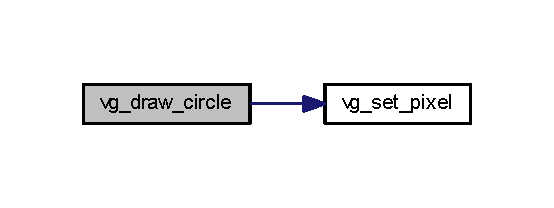
\includegraphics[width=266pt]{group__video__gr_ga0410a09b926582249fb7c0a795c9d4fe_cgraph}
\end{center}
\end{figure}
\hypertarget{group__video__gr_gafcdcee0785e2e5a0d0f1f460bf436403}{}\label{group__video__gr_gafcdcee0785e2e5a0d0f1f460bf436403} 
\index{video\+\_\+gr@{video\+\_\+gr}!vg\+\_\+draw\+\_\+square@{vg\+\_\+draw\+\_\+square}}
\index{vg\+\_\+draw\+\_\+square@{vg\+\_\+draw\+\_\+square}!video\+\_\+gr@{video\+\_\+gr}}
\subsubsection{\texorpdfstring{vg\+\_\+draw\+\_\+square()}{vg\_draw\_square()}}
{\footnotesize\ttfamily int vg\+\_\+draw\+\_\+square (\begin{DoxyParamCaption}\item[{int}]{xi,  }\item[{int}]{yi,  }\item[{int}]{size,  }\item[{int}]{color }\end{DoxyParamCaption})}



draws a square in the double buffer and in the mouse buffer 


\begin{DoxyParams}{Parameters}
{\em xi,yi} & coordinates of the superior left vertice of the square \\
\hline
{\em size} & size of the square \\
\hline
{\em color} & color of the square \\
\hline
\end{DoxyParams}
\begin{DoxyReturn}{Returns}
0 in case of success, 1 otherwise 
\end{DoxyReturn}
Here is the call graph for this function\+:\nopagebreak
\begin{figure}[H]
\begin{center}
\leavevmode
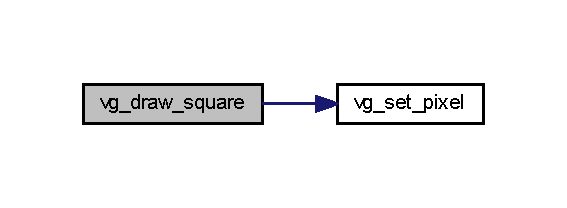
\includegraphics[width=272pt]{group__video__gr_gafcdcee0785e2e5a0d0f1f460bf436403_cgraph}
\end{center}
\end{figure}
\hypertarget{group__video__gr_ga42f593e6656f1a978315aff02b1bcebf}{}\label{group__video__gr_ga42f593e6656f1a978315aff02b1bcebf} 
\index{video\+\_\+gr@{video\+\_\+gr}!vg\+\_\+exit@{vg\+\_\+exit}}
\index{vg\+\_\+exit@{vg\+\_\+exit}!video\+\_\+gr@{video\+\_\+gr}}
\subsubsection{\texorpdfstring{vg\+\_\+exit()}{vg\_exit()}}
{\footnotesize\ttfamily int vg\+\_\+exit (\begin{DoxyParamCaption}\item[{void}]{ }\end{DoxyParamCaption})}



Returns to default Minix 3 text mode (0x03\+: 25 x 80, 16 colors) 

\begin{DoxyReturn}{Returns}
0 upon success, non-\/zero upon failure 
\end{DoxyReturn}
\hypertarget{group__video__gr_gacef21667c79365d57a084bed994c2189}{}\label{group__video__gr_gacef21667c79365d57a084bed994c2189} 
\index{video\+\_\+gr@{video\+\_\+gr}!vg\+\_\+init@{vg\+\_\+init}}
\index{vg\+\_\+init@{vg\+\_\+init}!video\+\_\+gr@{video\+\_\+gr}}
\subsubsection{\texorpdfstring{vg\+\_\+init()}{vg\_init()}}
{\footnotesize\ttfamily void$\ast$ vg\+\_\+init (\begin{DoxyParamCaption}\item[{unsigned short}]{mode }\end{DoxyParamCaption})}



Initializes the video module in graphics mode. 

Uses the V\+BE I\+NT 0x10 interface to set the desired graphics mode, maps V\+R\+AM to the process\textquotesingle{} address space and initializes static global variables with the resolution of the screen, and the number of colors


\begin{DoxyParams}{Parameters}
{\em mode} & 16-\/bit V\+BE mode to set \\
\hline
\end{DoxyParams}
\begin{DoxyReturn}{Returns}
Virtual address V\+R\+AM was mapped to. N\+U\+LL, upon failure. 
\end{DoxyReturn}
Here is the call graph for this function\+:
% FIG 0
\hypertarget{group__video__gr_ga78765c3e4634b79d0c27b464be410803}{}\label{group__video__gr_ga78765c3e4634b79d0c27b464be410803} 
\index{video\+\_\+gr@{video\+\_\+gr}!vg\+\_\+set\+\_\+mouse\+\_\+pixel@{vg\+\_\+set\+\_\+mouse\+\_\+pixel}}
\index{vg\+\_\+set\+\_\+mouse\+\_\+pixel@{vg\+\_\+set\+\_\+mouse\+\_\+pixel}!video\+\_\+gr@{video\+\_\+gr}}
\subsubsection{\texorpdfstring{vg\+\_\+set\+\_\+mouse\+\_\+pixel()}{vg\_set\_mouse\_pixel()}}
{\footnotesize\ttfamily int vg\+\_\+set\+\_\+mouse\+\_\+pixel (\begin{DoxyParamCaption}\item[{int}]{x,  }\item[{int}]{y,  }\item[{unsigned int}]{color }\end{DoxyParamCaption})}



sets the color of a pixel in the mouse buffer 


\begin{DoxyParams}{Parameters}
{\em x,y} & coordinates of the pixel we want to set \\
\hline
{\em color} & color which we want to set the pixel \\
\hline
\end{DoxyParams}
\begin{DoxyReturn}{Returns}
0 in case of success, 1 otherwise 
\end{DoxyReturn}
\hypertarget{group__video__gr_ga729c07175ab64956c7fd9944d7676888}{}\label{group__video__gr_ga729c07175ab64956c7fd9944d7676888} 
\index{video\+\_\+gr@{video\+\_\+gr}!vg\+\_\+set\+\_\+pixel@{vg\+\_\+set\+\_\+pixel}}
\index{vg\+\_\+set\+\_\+pixel@{vg\+\_\+set\+\_\+pixel}!video\+\_\+gr@{video\+\_\+gr}}
\subsubsection{\texorpdfstring{vg\+\_\+set\+\_\+pixel()}{vg\_set\_pixel()}}
{\footnotesize\ttfamily int vg\+\_\+set\+\_\+pixel (\begin{DoxyParamCaption}\item[{int}]{x,  }\item[{int}]{y,  }\item[{unsigned int}]{color }\end{DoxyParamCaption})}



sets the color of a pixel in the double buffer and in the mouse buffer 


\begin{DoxyParams}{Parameters}
{\em x,y} & coordinates of the pixel we want to set \\
\hline
{\em color} & color which we want to set the pixel \\
\hline
\end{DoxyParams}
\begin{DoxyReturn}{Returns}
0 in case of success, 1 otherwise 
\end{DoxyReturn}

\chapter{Data Structure Documentation}
\hypertarget{struct_bitmap}{}\section{Bitmap Struct Reference}
\label{struct_bitmap}\index{Bitmap@{Bitmap}}


{\ttfamily \#include $<$Bitmap.\+h$>$}



Collaboration diagram for Bitmap\+:\nopagebreak
\begin{figure}[H]
\begin{center}
\leavevmode
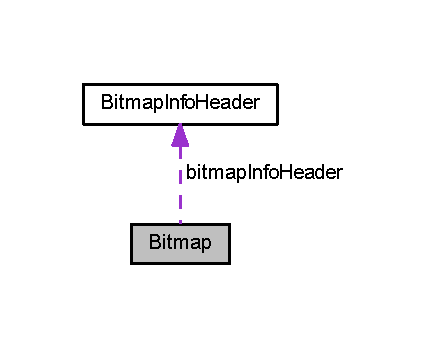
\includegraphics[width=206pt]{struct_bitmap__coll__graph}
\end{center}
\end{figure}
\subsection*{Data Fields}
\begin{DoxyCompactItemize}
\item 
\hyperlink{struct_bitmap_info_header}{Bitmap\+Info\+Header} \hyperlink{group___bitmap_ga7157ca7f3ce4be47481c472fafd89313}{bitmap\+Info\+Header}
\item 
unsigned char $\ast$ \hyperlink{group___bitmap_ga586c4bcc42cf22a033e8f60f24f627f0}{bitmap\+Data}
\end{DoxyCompactItemize}


\subsection{Detailed Description}
Represents a \hyperlink{struct_bitmap}{Bitmap} 

The documentation for this struct was generated from the following file\+:\begin{DoxyCompactItemize}
\item 
\hyperlink{_bitmap_8h}{Bitmap.\+h}\end{DoxyCompactItemize}

\hypertarget{struct_bitmap_file_header}{}\section{Bitmap\+File\+Header Struct Reference}
\label{struct_bitmap_file_header}\index{Bitmap\+File\+Header@{Bitmap\+File\+Header}}


{\ttfamily \#include $<$Bitmap.\+h$>$}

\subsection*{Data Fields}
\begin{DoxyCompactItemize}
\item 
unsigned short \hyperlink{group___bitmap_gaa929142c5ddf34cf0915c97a617a1a63}{type}
\begin{DoxyCompactList}\small\item\em specifies the file type \end{DoxyCompactList}\item 
unsigned int \hyperlink{group___bitmap_gaac913b3a1f6ef005d66bf7a84428773e}{size}
\begin{DoxyCompactList}\small\item\em specifies the size in bytes of the bitmap file \end{DoxyCompactList}\item 
unsigned int \hyperlink{group___bitmap_ga05d5cbcb44f437341bd9fa37d589aced}{reserved}
\begin{DoxyCompactList}\small\item\em reserved; must be 0 \end{DoxyCompactList}\item 
unsigned int \hyperlink{group___bitmap_ga29b5297d3393519050e3126c4cb07c1c}{offset}
\begin{DoxyCompactList}\small\item\em specifies the offset in bytes from the bitmapfileheader to the bitmap bits \end{DoxyCompactList}\end{DoxyCompactItemize}


The documentation for this struct was generated from the following file\+:\begin{DoxyCompactItemize}
\item 
\hyperlink{_bitmap_8h}{Bitmap.\+h}\end{DoxyCompactItemize}

\hypertarget{struct_bitmap_info_header}{}\section{Bitmap\+Info\+Header Struct Reference}
\label{struct_bitmap_info_header}\index{Bitmap\+Info\+Header@{Bitmap\+Info\+Header}}


{\ttfamily \#include $<$Bitmap.\+h$>$}

\subsection*{Data Fields}
\begin{DoxyCompactItemize}
\item 
unsigned int \hyperlink{group___bitmap_gaac913b3a1f6ef005d66bf7a84428773e}{size}
\begin{DoxyCompactList}\small\item\em specifies the number of bytes required by the struct \end{DoxyCompactList}\item 
int \hyperlink{group___bitmap_ga2474a5474cbff19523a51eb1de01cda4}{width}
\begin{DoxyCompactList}\small\item\em specifies width in pixels \end{DoxyCompactList}\item 
int \hyperlink{group___bitmap_gad12fc34ce789bce6c8a05d8a17138534}{height}
\begin{DoxyCompactList}\small\item\em specifies height in pixels \end{DoxyCompactList}\item 
unsigned short \hyperlink{group___bitmap_ga8c89d091e05544a82dc2398eed99634f}{planes}
\begin{DoxyCompactList}\small\item\em specifies the number of color planes, must be 1 \end{DoxyCompactList}\item 
unsigned short \hyperlink{group___bitmap_ga47d1d4d776f8fd3bb0f7dbc3c5aeb534}{bits}
\begin{DoxyCompactList}\small\item\em specifies the number of bit per pixel \end{DoxyCompactList}\item 
unsigned int \hyperlink{group___bitmap_gad180079f62b44e49ec672c9ef6e078b3}{compression}
\begin{DoxyCompactList}\small\item\em specifies the type of compression \end{DoxyCompactList}\item 
unsigned int \hyperlink{group___bitmap_gadcd57a0168319e747bc8099218d3822c}{image\+Size}
\begin{DoxyCompactList}\small\item\em size of image in bytes \end{DoxyCompactList}\item 
int \hyperlink{group___bitmap_gac6eaeb4c0876cf6cd899f41fe3c25ff5}{x\+Resolution}
\begin{DoxyCompactList}\small\item\em number of pixels per meter in x axis \end{DoxyCompactList}\item 
int \hyperlink{group___bitmap_gaa2f350dd0bda750656d5db5f5e37b2b3}{y\+Resolution}
\begin{DoxyCompactList}\small\item\em number of pixels per meter in y axis \end{DoxyCompactList}\item 
unsigned int \hyperlink{group___bitmap_gaed4506bad904845183194f199f1bdb98}{n\+Colors}
\begin{DoxyCompactList}\small\item\em number of colors used by the bitmap \end{DoxyCompactList}\item 
unsigned int \hyperlink{group___bitmap_ga8f7abfbc446b12f385d2b42c3b4fd9b0}{important\+Colors}
\begin{DoxyCompactList}\small\item\em number of colors that are important \end{DoxyCompactList}\end{DoxyCompactItemize}


The documentation for this struct was generated from the following file\+:\begin{DoxyCompactItemize}
\item 
\hyperlink{_bitmap_8h}{Bitmap.\+h}\end{DoxyCompactItemize}

\hypertarget{structdate__t}{}\section{date\+\_\+t Struct Reference}
\label{structdate__t}\index{date\+\_\+t@{date\+\_\+t}}


{\ttfamily \#include $<$rtc.\+h$>$}

\subsection*{Data Fields}
\begin{DoxyCompactItemize}
\item 
int \hyperlink{structdate__t_abeac221e38b7b9ce7df8722c842bf671}{year}
\item 
int \hyperlink{structdate__t_aedb06abe5aff12fa3e7e0e71a374edfb}{month}
\item 
int \hyperlink{structdate__t_a4c11afc03fc3ee49bab660def6558f2a}{day}
\end{DoxyCompactItemize}


\subsection{Field Documentation}
\hypertarget{structdate__t_a4c11afc03fc3ee49bab660def6558f2a}{}\label{structdate__t_a4c11afc03fc3ee49bab660def6558f2a} 
\index{date\+\_\+t@{date\+\_\+t}!day@{day}}
\index{day@{day}!date\+\_\+t@{date\+\_\+t}}
\subsubsection{\texorpdfstring{day}{day}}
{\footnotesize\ttfamily int day}

\hypertarget{structdate__t_aedb06abe5aff12fa3e7e0e71a374edfb}{}\label{structdate__t_aedb06abe5aff12fa3e7e0e71a374edfb} 
\index{date\+\_\+t@{date\+\_\+t}!month@{month}}
\index{month@{month}!date\+\_\+t@{date\+\_\+t}}
\subsubsection{\texorpdfstring{month}{month}}
{\footnotesize\ttfamily int month}

\hypertarget{structdate__t_abeac221e38b7b9ce7df8722c842bf671}{}\label{structdate__t_abeac221e38b7b9ce7df8722c842bf671} 
\index{date\+\_\+t@{date\+\_\+t}!year@{year}}
\index{year@{year}!date\+\_\+t@{date\+\_\+t}}
\subsubsection{\texorpdfstring{year}{year}}
{\footnotesize\ttfamily int year}



The documentation for this struct was generated from the following file\+:\begin{DoxyCompactItemize}
\item 
\hyperlink{rtc_8h}{rtc.\+h}\end{DoxyCompactItemize}

\hypertarget{structmmap__t}{}\section{mmap\+\_\+t Struct Reference}
\label{structmmap__t}\index{mmap\+\_\+t@{mmap\+\_\+t}}


Memory Map Struct.  




{\ttfamily \#include $<$lmlib.\+h$>$}

\subsection*{Data Fields}
\begin{DoxyCompactItemize}
\item 
phys\+\_\+bytes \hyperlink{group__lmlib_gab7a85fe0db943529016cf606e3a7167f}{phys}
\begin{DoxyCompactList}\small\item\em physical address \end{DoxyCompactList}\item 
void $\ast$ \hyperlink{group__lmlib_ga6a0ea2231d30f2b025e0c4b9f12dd6db}{virtual}
\begin{DoxyCompactList}\small\item\em virtual address \end{DoxyCompactList}\item 
unsigned long \hyperlink{group__lmlib_ga1e1268d164c38e4f8a4f4eb9058b0601}{size}
\begin{DoxyCompactList}\small\item\em size of memory region \end{DoxyCompactList}\end{DoxyCompactItemize}


\subsection{Detailed Description}
Memory Map Struct. 

Struct that keeps info regarding the mapping of physical memory to virtual memory 

The documentation for this struct was generated from the following file\+:\begin{DoxyCompactItemize}
\item 
\hyperlink{lmlib_8h}{lmlib.\+h}\end{DoxyCompactItemize}

\hypertarget{structmouse__packet__t}{}\section{mouse\+\_\+packet\+\_\+t Struct Reference}
\label{structmouse__packet__t}\index{mouse\+\_\+packet\+\_\+t@{mouse\+\_\+packet\+\_\+t}}


{\ttfamily \#include $<$mouse.\+h$>$}

\subsection*{Data Fields}
\begin{DoxyCompactItemize}
\item 
char \hyperlink{structmouse__packet__t_a5c19008eeede220db3123a269f5efd21}{lb}
\begin{DoxyCompactList}\small\item\em 1 if left button is pressed, 0 otherwise \end{DoxyCompactList}\item 
char \hyperlink{structmouse__packet__t_a2923f784f55df16ef02f4db7ea172b33}{mb}
\begin{DoxyCompactList}\small\item\em 1 if middle button is pressed, 0 otherwise \end{DoxyCompactList}\item 
char \hyperlink{structmouse__packet__t_ad2b989ebf6f8d10ba3501f5c464f37e6}{rb}
\begin{DoxyCompactList}\small\item\em 1 if right button is pressed, 0 otherwise \end{DoxyCompactList}\item 
int \hyperlink{structmouse__packet__t_a6150e0515f7202e2fb518f7206ed97dc}{x}
\begin{DoxyCompactList}\small\item\em value of the x movement \end{DoxyCompactList}\item 
int \hyperlink{structmouse__packet__t_a0a2f84ed7838f07779ae24c5a9086d33}{y}
\begin{DoxyCompactList}\small\item\em value of the y movement \end{DoxyCompactList}\end{DoxyCompactItemize}


\subsection{Field Documentation}
\hypertarget{structmouse__packet__t_a5c19008eeede220db3123a269f5efd21}{}\label{structmouse__packet__t_a5c19008eeede220db3123a269f5efd21} 
\index{mouse\+\_\+packet\+\_\+t@{mouse\+\_\+packet\+\_\+t}!lb@{lb}}
\index{lb@{lb}!mouse\+\_\+packet\+\_\+t@{mouse\+\_\+packet\+\_\+t}}
\subsubsection{\texorpdfstring{lb}{lb}}
{\footnotesize\ttfamily char lb}



1 if left button is pressed, 0 otherwise 

\hypertarget{structmouse__packet__t_a2923f784f55df16ef02f4db7ea172b33}{}\label{structmouse__packet__t_a2923f784f55df16ef02f4db7ea172b33} 
\index{mouse\+\_\+packet\+\_\+t@{mouse\+\_\+packet\+\_\+t}!mb@{mb}}
\index{mb@{mb}!mouse\+\_\+packet\+\_\+t@{mouse\+\_\+packet\+\_\+t}}
\subsubsection{\texorpdfstring{mb}{mb}}
{\footnotesize\ttfamily char mb}



1 if middle button is pressed, 0 otherwise 

\hypertarget{structmouse__packet__t_ad2b989ebf6f8d10ba3501f5c464f37e6}{}\label{structmouse__packet__t_ad2b989ebf6f8d10ba3501f5c464f37e6} 
\index{mouse\+\_\+packet\+\_\+t@{mouse\+\_\+packet\+\_\+t}!rb@{rb}}
\index{rb@{rb}!mouse\+\_\+packet\+\_\+t@{mouse\+\_\+packet\+\_\+t}}
\subsubsection{\texorpdfstring{rb}{rb}}
{\footnotesize\ttfamily char rb}



1 if right button is pressed, 0 otherwise 

\hypertarget{structmouse__packet__t_a6150e0515f7202e2fb518f7206ed97dc}{}\label{structmouse__packet__t_a6150e0515f7202e2fb518f7206ed97dc} 
\index{mouse\+\_\+packet\+\_\+t@{mouse\+\_\+packet\+\_\+t}!x@{x}}
\index{x@{x}!mouse\+\_\+packet\+\_\+t@{mouse\+\_\+packet\+\_\+t}}
\subsubsection{\texorpdfstring{x}{x}}
{\footnotesize\ttfamily int x}



value of the x movement 

\hypertarget{structmouse__packet__t_a0a2f84ed7838f07779ae24c5a9086d33}{}\label{structmouse__packet__t_a0a2f84ed7838f07779ae24c5a9086d33} 
\index{mouse\+\_\+packet\+\_\+t@{mouse\+\_\+packet\+\_\+t}!y@{y}}
\index{y@{y}!mouse\+\_\+packet\+\_\+t@{mouse\+\_\+packet\+\_\+t}}
\subsubsection{\texorpdfstring{y}{y}}
{\footnotesize\ttfamily int y}



value of the y movement 



The documentation for this struct was generated from the following file\+:\begin{DoxyCompactItemize}
\item 
\hyperlink{mouse_8h}{mouse.\+h}\end{DoxyCompactItemize}

\hypertarget{structmouse__t}{}\section{mouse\+\_\+t Struct Reference}
\label{structmouse__t}\index{mouse\+\_\+t@{mouse\+\_\+t}}


{\ttfamily \#include $<$checkers.\+h$>$}



Collaboration diagram for mouse\+\_\+t\+:\nopagebreak
\begin{figure}[H]
\begin{center}
\leavevmode
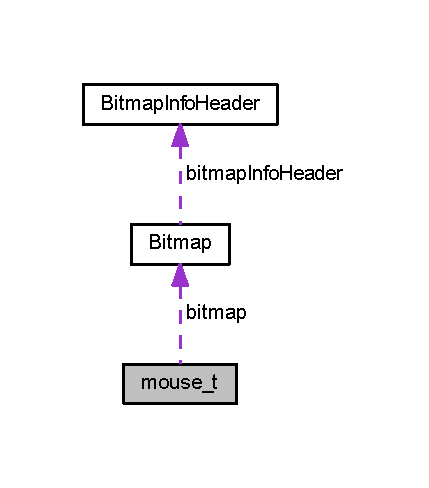
\includegraphics[width=206pt]{structmouse__t__coll__graph}
\end{center}
\end{figure}
\subsection*{Data Fields}
\begin{DoxyCompactItemize}
\item 
int \hyperlink{structmouse__t_a6150e0515f7202e2fb518f7206ed97dc}{x}
\item 
int \hyperlink{structmouse__t_a0a2f84ed7838f07779ae24c5a9086d33}{y}
\item 
\hyperlink{struct_bitmap}{Bitmap} $\ast$ \hyperlink{structmouse__t_a00c870e2cedff0b231b1c8ad85019f66}{bitmap}
\item 
int \hyperlink{structmouse__t_a0c4545c1a96c0145f5a3c908f1df2b8a}{hold}
\item 
int \hyperlink{structmouse__t_a395279899207ce7f17adf9fdb8ee97ee}{radius}
\item 
int \hyperlink{structmouse__t_a1167d2ae386ab6d548a086185e16a43b}{color\+\_\+circle}
\item 
int \hyperlink{structmouse__t_af8ae0e3b70fa87729bedfdb24414857e}{x\+\_\+circle}
\item 
int \hyperlink{structmouse__t_ad7206eb221c616f2208152a59b62eb1d}{y\+\_\+circle}
\item 
int \hyperlink{structmouse__t_a4f08f62253e9d13c564b88256150c0dd}{original\+\_\+x}
\item 
int \hyperlink{structmouse__t_a9ae97019274f18be94e95d77c4adcf3d}{original\+\_\+y}
\end{DoxyCompactItemize}


\subsection{Detailed Description}
This struct represents the mouse that will be used to play checkers 

\subsection{Field Documentation}
\hypertarget{structmouse__t_a00c870e2cedff0b231b1c8ad85019f66}{}\label{structmouse__t_a00c870e2cedff0b231b1c8ad85019f66} 
\index{mouse\+\_\+t@{mouse\+\_\+t}!bitmap@{bitmap}}
\index{bitmap@{bitmap}!mouse\+\_\+t@{mouse\+\_\+t}}
\subsubsection{\texorpdfstring{bitmap}{bitmap}}
{\footnotesize\ttfamily \hyperlink{struct_bitmap}{Bitmap}$\ast$ bitmap}

\hypertarget{structmouse__t_a1167d2ae386ab6d548a086185e16a43b}{}\label{structmouse__t_a1167d2ae386ab6d548a086185e16a43b} 
\index{mouse\+\_\+t@{mouse\+\_\+t}!color\+\_\+circle@{color\+\_\+circle}}
\index{color\+\_\+circle@{color\+\_\+circle}!mouse\+\_\+t@{mouse\+\_\+t}}
\subsubsection{\texorpdfstring{color\+\_\+circle}{color\_circle}}
{\footnotesize\ttfamily int color\+\_\+circle}

\hypertarget{structmouse__t_a0c4545c1a96c0145f5a3c908f1df2b8a}{}\label{structmouse__t_a0c4545c1a96c0145f5a3c908f1df2b8a} 
\index{mouse\+\_\+t@{mouse\+\_\+t}!hold@{hold}}
\index{hold@{hold}!mouse\+\_\+t@{mouse\+\_\+t}}
\subsubsection{\texorpdfstring{hold}{hold}}
{\footnotesize\ttfamily int hold}

\hypertarget{structmouse__t_a4f08f62253e9d13c564b88256150c0dd}{}\label{structmouse__t_a4f08f62253e9d13c564b88256150c0dd} 
\index{mouse\+\_\+t@{mouse\+\_\+t}!original\+\_\+x@{original\+\_\+x}}
\index{original\+\_\+x@{original\+\_\+x}!mouse\+\_\+t@{mouse\+\_\+t}}
\subsubsection{\texorpdfstring{original\+\_\+x}{original\_x}}
{\footnotesize\ttfamily int original\+\_\+x}

\hypertarget{structmouse__t_a9ae97019274f18be94e95d77c4adcf3d}{}\label{structmouse__t_a9ae97019274f18be94e95d77c4adcf3d} 
\index{mouse\+\_\+t@{mouse\+\_\+t}!original\+\_\+y@{original\+\_\+y}}
\index{original\+\_\+y@{original\+\_\+y}!mouse\+\_\+t@{mouse\+\_\+t}}
\subsubsection{\texorpdfstring{original\+\_\+y}{original\_y}}
{\footnotesize\ttfamily int original\+\_\+y}

\hypertarget{structmouse__t_a395279899207ce7f17adf9fdb8ee97ee}{}\label{structmouse__t_a395279899207ce7f17adf9fdb8ee97ee} 
\index{mouse\+\_\+t@{mouse\+\_\+t}!radius@{radius}}
\index{radius@{radius}!mouse\+\_\+t@{mouse\+\_\+t}}
\subsubsection{\texorpdfstring{radius}{radius}}
{\footnotesize\ttfamily int radius}

\hypertarget{structmouse__t_a6150e0515f7202e2fb518f7206ed97dc}{}\label{structmouse__t_a6150e0515f7202e2fb518f7206ed97dc} 
\index{mouse\+\_\+t@{mouse\+\_\+t}!x@{x}}
\index{x@{x}!mouse\+\_\+t@{mouse\+\_\+t}}
\subsubsection{\texorpdfstring{x}{x}}
{\footnotesize\ttfamily int x}

\hypertarget{structmouse__t_af8ae0e3b70fa87729bedfdb24414857e}{}\label{structmouse__t_af8ae0e3b70fa87729bedfdb24414857e} 
\index{mouse\+\_\+t@{mouse\+\_\+t}!x\+\_\+circle@{x\+\_\+circle}}
\index{x\+\_\+circle@{x\+\_\+circle}!mouse\+\_\+t@{mouse\+\_\+t}}
\subsubsection{\texorpdfstring{x\+\_\+circle}{x\_circle}}
{\footnotesize\ttfamily int x\+\_\+circle}

\hypertarget{structmouse__t_a0a2f84ed7838f07779ae24c5a9086d33}{}\label{structmouse__t_a0a2f84ed7838f07779ae24c5a9086d33} 
\index{mouse\+\_\+t@{mouse\+\_\+t}!y@{y}}
\index{y@{y}!mouse\+\_\+t@{mouse\+\_\+t}}
\subsubsection{\texorpdfstring{y}{y}}
{\footnotesize\ttfamily int y}

\hypertarget{structmouse__t_ad7206eb221c616f2208152a59b62eb1d}{}\label{structmouse__t_ad7206eb221c616f2208152a59b62eb1d} 
\index{mouse\+\_\+t@{mouse\+\_\+t}!y\+\_\+circle@{y\+\_\+circle}}
\index{y\+\_\+circle@{y\+\_\+circle}!mouse\+\_\+t@{mouse\+\_\+t}}
\subsubsection{\texorpdfstring{y\+\_\+circle}{y\_circle}}
{\footnotesize\ttfamily int y\+\_\+circle}



The documentation for this struct was generated from the following file\+:\begin{DoxyCompactItemize}
\item 
\hyperlink{checkers_8h}{checkers.\+h}\end{DoxyCompactItemize}

\hypertarget{structser__conf__t}{}\section{ser\+\_\+conf\+\_\+t Struct Reference}
\label{structser__conf__t}\index{ser\+\_\+conf\+\_\+t@{ser\+\_\+conf\+\_\+t}}


{\ttfamily \#include $<$ser\+\_\+port.\+h$>$}

\subsection*{Data Fields}
\begin{DoxyCompactItemize}
\item 
int \hyperlink{structser__conf__t_a542331bcc7806df403a7210e40382b89}{bits\+\_\+per\+\_\+char}
\begin{DoxyCompactList}\small\item\em number of bits per char \end{DoxyCompactList}\item 
int \hyperlink{structser__conf__t_a146991e1ecc6d049155a7a71739e9d0d}{stop\+\_\+bits}
\begin{DoxyCompactList}\small\item\em number of stop bits \end{DoxyCompactList}\item 
char \hyperlink{structser__conf__t_a0674046773a72bb7d71956cd58d393a9}{parity} \mbox{[}10\mbox{]}
\begin{DoxyCompactList}\small\item\em parity \end{DoxyCompactList}\item 
int \hyperlink{structser__conf__t_a7a829e6fd74e94e0edf10550470d844c}{rate}
\begin{DoxyCompactList}\small\item\em rate \end{DoxyCompactList}\item 
int \hyperlink{structser__conf__t_a98c7ee45de40e6a45659762a1fb66830}{rec\+\_\+data\+\_\+intpt}
\begin{DoxyCompactList}\small\item\em this variable is set to 1 if this interrupt is enabled \end{DoxyCompactList}\item 
int \hyperlink{structser__conf__t_ada0c84c6581ba1cfae8bd5e3ee17443a}{trans\+\_\+empty\+\_\+intpt}
\begin{DoxyCompactList}\small\item\em this variable is set to 1 if this interrupt is enabled \end{DoxyCompactList}\item 
int \hyperlink{structser__conf__t_a95598f55f1281cb9f1b46ee311fe793e}{rec\+\_\+line\+\_\+stat\+\_\+intpt}
\begin{DoxyCompactList}\small\item\em this variable is set to 1 if this interrupt is enabled \end{DoxyCompactList}\end{DoxyCompactItemize}


\subsection{Detailed Description}
Struct that represents the configuration of an U\+A\+RT 

\subsection{Field Documentation}
\hypertarget{structser__conf__t_a542331bcc7806df403a7210e40382b89}{}\label{structser__conf__t_a542331bcc7806df403a7210e40382b89} 
\index{ser\+\_\+conf\+\_\+t@{ser\+\_\+conf\+\_\+t}!bits\+\_\+per\+\_\+char@{bits\+\_\+per\+\_\+char}}
\index{bits\+\_\+per\+\_\+char@{bits\+\_\+per\+\_\+char}!ser\+\_\+conf\+\_\+t@{ser\+\_\+conf\+\_\+t}}
\subsubsection{\texorpdfstring{bits\+\_\+per\+\_\+char}{bits\_per\_char}}
{\footnotesize\ttfamily int bits\+\_\+per\+\_\+char}



number of bits per char 

\hypertarget{structser__conf__t_a0674046773a72bb7d71956cd58d393a9}{}\label{structser__conf__t_a0674046773a72bb7d71956cd58d393a9} 
\index{ser\+\_\+conf\+\_\+t@{ser\+\_\+conf\+\_\+t}!parity@{parity}}
\index{parity@{parity}!ser\+\_\+conf\+\_\+t@{ser\+\_\+conf\+\_\+t}}
\subsubsection{\texorpdfstring{parity}{parity}}
{\footnotesize\ttfamily char parity\mbox{[}10\mbox{]}}



parity 

\hypertarget{structser__conf__t_a7a829e6fd74e94e0edf10550470d844c}{}\label{structser__conf__t_a7a829e6fd74e94e0edf10550470d844c} 
\index{ser\+\_\+conf\+\_\+t@{ser\+\_\+conf\+\_\+t}!rate@{rate}}
\index{rate@{rate}!ser\+\_\+conf\+\_\+t@{ser\+\_\+conf\+\_\+t}}
\subsubsection{\texorpdfstring{rate}{rate}}
{\footnotesize\ttfamily int rate}



rate 

\hypertarget{structser__conf__t_a98c7ee45de40e6a45659762a1fb66830}{}\label{structser__conf__t_a98c7ee45de40e6a45659762a1fb66830} 
\index{ser\+\_\+conf\+\_\+t@{ser\+\_\+conf\+\_\+t}!rec\+\_\+data\+\_\+intpt@{rec\+\_\+data\+\_\+intpt}}
\index{rec\+\_\+data\+\_\+intpt@{rec\+\_\+data\+\_\+intpt}!ser\+\_\+conf\+\_\+t@{ser\+\_\+conf\+\_\+t}}
\subsubsection{\texorpdfstring{rec\+\_\+data\+\_\+intpt}{rec\_data\_intpt}}
{\footnotesize\ttfamily int rec\+\_\+data\+\_\+intpt}



this variable is set to 1 if this interrupt is enabled 

\hypertarget{structser__conf__t_a95598f55f1281cb9f1b46ee311fe793e}{}\label{structser__conf__t_a95598f55f1281cb9f1b46ee311fe793e} 
\index{ser\+\_\+conf\+\_\+t@{ser\+\_\+conf\+\_\+t}!rec\+\_\+line\+\_\+stat\+\_\+intpt@{rec\+\_\+line\+\_\+stat\+\_\+intpt}}
\index{rec\+\_\+line\+\_\+stat\+\_\+intpt@{rec\+\_\+line\+\_\+stat\+\_\+intpt}!ser\+\_\+conf\+\_\+t@{ser\+\_\+conf\+\_\+t}}
\subsubsection{\texorpdfstring{rec\+\_\+line\+\_\+stat\+\_\+intpt}{rec\_line\_stat\_intpt}}
{\footnotesize\ttfamily int rec\+\_\+line\+\_\+stat\+\_\+intpt}



this variable is set to 1 if this interrupt is enabled 

\hypertarget{structser__conf__t_a146991e1ecc6d049155a7a71739e9d0d}{}\label{structser__conf__t_a146991e1ecc6d049155a7a71739e9d0d} 
\index{ser\+\_\+conf\+\_\+t@{ser\+\_\+conf\+\_\+t}!stop\+\_\+bits@{stop\+\_\+bits}}
\index{stop\+\_\+bits@{stop\+\_\+bits}!ser\+\_\+conf\+\_\+t@{ser\+\_\+conf\+\_\+t}}
\subsubsection{\texorpdfstring{stop\+\_\+bits}{stop\_bits}}
{\footnotesize\ttfamily int stop\+\_\+bits}



number of stop bits 

\hypertarget{structser__conf__t_ada0c84c6581ba1cfae8bd5e3ee17443a}{}\label{structser__conf__t_ada0c84c6581ba1cfae8bd5e3ee17443a} 
\index{ser\+\_\+conf\+\_\+t@{ser\+\_\+conf\+\_\+t}!trans\+\_\+empty\+\_\+intpt@{trans\+\_\+empty\+\_\+intpt}}
\index{trans\+\_\+empty\+\_\+intpt@{trans\+\_\+empty\+\_\+intpt}!ser\+\_\+conf\+\_\+t@{ser\+\_\+conf\+\_\+t}}
\subsubsection{\texorpdfstring{trans\+\_\+empty\+\_\+intpt}{trans\_empty\_intpt}}
{\footnotesize\ttfamily int trans\+\_\+empty\+\_\+intpt}



this variable is set to 1 if this interrupt is enabled 



The documentation for this struct was generated from the following file\+:\begin{DoxyCompactItemize}
\item 
\hyperlink{ser__port_8h}{ser\+\_\+port.\+h}\end{DoxyCompactItemize}

\hypertarget{structvbe__info__block__t}{}\section{vbe\+\_\+info\+\_\+block\+\_\+t Struct Reference}
\label{structvbe__info__block__t}\index{vbe\+\_\+info\+\_\+block\+\_\+t@{vbe\+\_\+info\+\_\+block\+\_\+t}}


{\ttfamily \#include $<$vbe.\+h$>$}

\subsection*{Data Fields}
\begin{DoxyCompactItemize}
\item 
uint8\+\_\+t \hyperlink{structvbe__info__block__t_ae619d4d52ca296b56a18c6ec13d4899d}{Vbe\+Signature} \mbox{[}4\mbox{]}
\begin{DoxyCompactList}\small\item\em V\+BE Signature. \end{DoxyCompactList}\item 
uint16\+\_\+t \hyperlink{structvbe__info__block__t_a7b9fef89774326b46f9481cbd9a397d3}{Vbe\+Version}
\begin{DoxyCompactList}\small\item\em V\+BE Version. \end{DoxyCompactList}\item 
phys\+\_\+bytes \hyperlink{structvbe__info__block__t_a20ab55e9dda8d437875255529c1cffe8}{Oem\+String\+Ptr}
\begin{DoxyCompactList}\small\item\em Pointer to O\+EM String. \end{DoxyCompactList}\item 
uint8\+\_\+t \hyperlink{structvbe__info__block__t_a555521aede0ff448231fc7a404862bdb}{Capabilities} \mbox{[}4\mbox{]}
\begin{DoxyCompactList}\small\item\em Capabilities of graphics controller. \end{DoxyCompactList}\item 
phys\+\_\+bytes \hyperlink{structvbe__info__block__t_a9d989fdbcdad6a40c10fc28c0f9af760}{Video\+Mode\+Ptr}
\begin{DoxyCompactList}\small\item\em Pointer to Video\+Mode\+List. \end{DoxyCompactList}\item 
uint16\+\_\+t \hyperlink{structvbe__info__block__t_a3e7b41e709394a10b3667e7f27f1aa7a}{Total\+Memory}
\begin{DoxyCompactList}\small\item\em Number of 64kb memory blocks. \end{DoxyCompactList}\item 
uint16\+\_\+t \hyperlink{structvbe__info__block__t_a050873b740536c3f9c9a9b0ecb76b497}{Oem\+Software\+Rex}
\begin{DoxyCompactList}\small\item\em V\+BE implementation Software revision. \end{DoxyCompactList}\item 
phys\+\_\+bytes \hyperlink{structvbe__info__block__t_affd3a330afde841405f89bbcd05af4f0}{Oem\+Vendor\+Name\+Ptr}
\begin{DoxyCompactList}\small\item\em Pointer to Vendor Name String. \end{DoxyCompactList}\item 
phys\+\_\+bytes \hyperlink{structvbe__info__block__t_afd3d28c2078a683b1ed64ea21905fcfe}{Oem\+Product\+Name\+Ptr}
\begin{DoxyCompactList}\small\item\em Pointer to Product Name String. \end{DoxyCompactList}\item 
phys\+\_\+bytes \hyperlink{structvbe__info__block__t_a239cba41d0489da5b79556b45797c6b0}{Oem\+Product\+Rev\+Ptr}
\begin{DoxyCompactList}\small\item\em Pointer to Product Revision String. \end{DoxyCompactList}\item 
uint8\+\_\+t \hyperlink{structvbe__info__block__t_a2c3b1cbb6bad5c51d4be4e57255a61d2}{Reserved} \mbox{[}222\mbox{]}
\begin{DoxyCompactList}\small\item\em Reserved for V\+BE implementation scratch. \end{DoxyCompactList}\item 
uint8\+\_\+t \hyperlink{structvbe__info__block__t_a966ae75c33c2d65b4f0c916f093acac0}{Oem\+Data} \mbox{[}256\mbox{]}
\begin{DoxyCompactList}\small\item\em Data Area for O\+EM Strings. \end{DoxyCompactList}\end{DoxyCompactItemize}


\subsection{Detailed Description}
Vbe\+Info\+Block struct 

\subsection{Field Documentation}
\hypertarget{structvbe__info__block__t_a555521aede0ff448231fc7a404862bdb}{}\label{structvbe__info__block__t_a555521aede0ff448231fc7a404862bdb} 
\index{vbe\+\_\+info\+\_\+block\+\_\+t@{vbe\+\_\+info\+\_\+block\+\_\+t}!Capabilities@{Capabilities}}
\index{Capabilities@{Capabilities}!vbe\+\_\+info\+\_\+block\+\_\+t@{vbe\+\_\+info\+\_\+block\+\_\+t}}
\subsubsection{\texorpdfstring{Capabilities}{Capabilities}}
{\footnotesize\ttfamily uint8\+\_\+t Capabilities\mbox{[}4\mbox{]}}



Capabilities of graphics controller. 

\hypertarget{structvbe__info__block__t_a966ae75c33c2d65b4f0c916f093acac0}{}\label{structvbe__info__block__t_a966ae75c33c2d65b4f0c916f093acac0} 
\index{vbe\+\_\+info\+\_\+block\+\_\+t@{vbe\+\_\+info\+\_\+block\+\_\+t}!Oem\+Data@{Oem\+Data}}
\index{Oem\+Data@{Oem\+Data}!vbe\+\_\+info\+\_\+block\+\_\+t@{vbe\+\_\+info\+\_\+block\+\_\+t}}
\subsubsection{\texorpdfstring{Oem\+Data}{OemData}}
{\footnotesize\ttfamily uint8\+\_\+t Oem\+Data\mbox{[}256\mbox{]}}



Data Area for O\+EM Strings. 

\hypertarget{structvbe__info__block__t_afd3d28c2078a683b1ed64ea21905fcfe}{}\label{structvbe__info__block__t_afd3d28c2078a683b1ed64ea21905fcfe} 
\index{vbe\+\_\+info\+\_\+block\+\_\+t@{vbe\+\_\+info\+\_\+block\+\_\+t}!Oem\+Product\+Name\+Ptr@{Oem\+Product\+Name\+Ptr}}
\index{Oem\+Product\+Name\+Ptr@{Oem\+Product\+Name\+Ptr}!vbe\+\_\+info\+\_\+block\+\_\+t@{vbe\+\_\+info\+\_\+block\+\_\+t}}
\subsubsection{\texorpdfstring{Oem\+Product\+Name\+Ptr}{OemProductNamePtr}}
{\footnotesize\ttfamily phys\+\_\+bytes Oem\+Product\+Name\+Ptr}



Pointer to Product Name String. 

\hypertarget{structvbe__info__block__t_a239cba41d0489da5b79556b45797c6b0}{}\label{structvbe__info__block__t_a239cba41d0489da5b79556b45797c6b0} 
\index{vbe\+\_\+info\+\_\+block\+\_\+t@{vbe\+\_\+info\+\_\+block\+\_\+t}!Oem\+Product\+Rev\+Ptr@{Oem\+Product\+Rev\+Ptr}}
\index{Oem\+Product\+Rev\+Ptr@{Oem\+Product\+Rev\+Ptr}!vbe\+\_\+info\+\_\+block\+\_\+t@{vbe\+\_\+info\+\_\+block\+\_\+t}}
\subsubsection{\texorpdfstring{Oem\+Product\+Rev\+Ptr}{OemProductRevPtr}}
{\footnotesize\ttfamily phys\+\_\+bytes Oem\+Product\+Rev\+Ptr}



Pointer to Product Revision String. 

\hypertarget{structvbe__info__block__t_a050873b740536c3f9c9a9b0ecb76b497}{}\label{structvbe__info__block__t_a050873b740536c3f9c9a9b0ecb76b497} 
\index{vbe\+\_\+info\+\_\+block\+\_\+t@{vbe\+\_\+info\+\_\+block\+\_\+t}!Oem\+Software\+Rex@{Oem\+Software\+Rex}}
\index{Oem\+Software\+Rex@{Oem\+Software\+Rex}!vbe\+\_\+info\+\_\+block\+\_\+t@{vbe\+\_\+info\+\_\+block\+\_\+t}}
\subsubsection{\texorpdfstring{Oem\+Software\+Rex}{OemSoftwareRex}}
{\footnotesize\ttfamily uint16\+\_\+t Oem\+Software\+Rex}



V\+BE implementation Software revision. 

\hypertarget{structvbe__info__block__t_a20ab55e9dda8d437875255529c1cffe8}{}\label{structvbe__info__block__t_a20ab55e9dda8d437875255529c1cffe8} 
\index{vbe\+\_\+info\+\_\+block\+\_\+t@{vbe\+\_\+info\+\_\+block\+\_\+t}!Oem\+String\+Ptr@{Oem\+String\+Ptr}}
\index{Oem\+String\+Ptr@{Oem\+String\+Ptr}!vbe\+\_\+info\+\_\+block\+\_\+t@{vbe\+\_\+info\+\_\+block\+\_\+t}}
\subsubsection{\texorpdfstring{Oem\+String\+Ptr}{OemStringPtr}}
{\footnotesize\ttfamily phys\+\_\+bytes Oem\+String\+Ptr}



Pointer to O\+EM String. 

\hypertarget{structvbe__info__block__t_affd3a330afde841405f89bbcd05af4f0}{}\label{structvbe__info__block__t_affd3a330afde841405f89bbcd05af4f0} 
\index{vbe\+\_\+info\+\_\+block\+\_\+t@{vbe\+\_\+info\+\_\+block\+\_\+t}!Oem\+Vendor\+Name\+Ptr@{Oem\+Vendor\+Name\+Ptr}}
\index{Oem\+Vendor\+Name\+Ptr@{Oem\+Vendor\+Name\+Ptr}!vbe\+\_\+info\+\_\+block\+\_\+t@{vbe\+\_\+info\+\_\+block\+\_\+t}}
\subsubsection{\texorpdfstring{Oem\+Vendor\+Name\+Ptr}{OemVendorNamePtr}}
{\footnotesize\ttfamily phys\+\_\+bytes Oem\+Vendor\+Name\+Ptr}



Pointer to Vendor Name String. 

\hypertarget{structvbe__info__block__t_a2c3b1cbb6bad5c51d4be4e57255a61d2}{}\label{structvbe__info__block__t_a2c3b1cbb6bad5c51d4be4e57255a61d2} 
\index{vbe\+\_\+info\+\_\+block\+\_\+t@{vbe\+\_\+info\+\_\+block\+\_\+t}!Reserved@{Reserved}}
\index{Reserved@{Reserved}!vbe\+\_\+info\+\_\+block\+\_\+t@{vbe\+\_\+info\+\_\+block\+\_\+t}}
\subsubsection{\texorpdfstring{Reserved}{Reserved}}
{\footnotesize\ttfamily uint8\+\_\+t Reserved\mbox{[}222\mbox{]}}



Reserved for V\+BE implementation scratch. 

\hypertarget{structvbe__info__block__t_a3e7b41e709394a10b3667e7f27f1aa7a}{}\label{structvbe__info__block__t_a3e7b41e709394a10b3667e7f27f1aa7a} 
\index{vbe\+\_\+info\+\_\+block\+\_\+t@{vbe\+\_\+info\+\_\+block\+\_\+t}!Total\+Memory@{Total\+Memory}}
\index{Total\+Memory@{Total\+Memory}!vbe\+\_\+info\+\_\+block\+\_\+t@{vbe\+\_\+info\+\_\+block\+\_\+t}}
\subsubsection{\texorpdfstring{Total\+Memory}{TotalMemory}}
{\footnotesize\ttfamily uint16\+\_\+t Total\+Memory}



Number of 64kb memory blocks. 

\hypertarget{structvbe__info__block__t_ae619d4d52ca296b56a18c6ec13d4899d}{}\label{structvbe__info__block__t_ae619d4d52ca296b56a18c6ec13d4899d} 
\index{vbe\+\_\+info\+\_\+block\+\_\+t@{vbe\+\_\+info\+\_\+block\+\_\+t}!Vbe\+Signature@{Vbe\+Signature}}
\index{Vbe\+Signature@{Vbe\+Signature}!vbe\+\_\+info\+\_\+block\+\_\+t@{vbe\+\_\+info\+\_\+block\+\_\+t}}
\subsubsection{\texorpdfstring{Vbe\+Signature}{VbeSignature}}
{\footnotesize\ttfamily uint8\+\_\+t Vbe\+Signature\mbox{[}4\mbox{]}}



V\+BE Signature. 

\hypertarget{structvbe__info__block__t_a7b9fef89774326b46f9481cbd9a397d3}{}\label{structvbe__info__block__t_a7b9fef89774326b46f9481cbd9a397d3} 
\index{vbe\+\_\+info\+\_\+block\+\_\+t@{vbe\+\_\+info\+\_\+block\+\_\+t}!Vbe\+Version@{Vbe\+Version}}
\index{Vbe\+Version@{Vbe\+Version}!vbe\+\_\+info\+\_\+block\+\_\+t@{vbe\+\_\+info\+\_\+block\+\_\+t}}
\subsubsection{\texorpdfstring{Vbe\+Version}{VbeVersion}}
{\footnotesize\ttfamily uint16\+\_\+t Vbe\+Version}



V\+BE Version. 

\hypertarget{structvbe__info__block__t_a9d989fdbcdad6a40c10fc28c0f9af760}{}\label{structvbe__info__block__t_a9d989fdbcdad6a40c10fc28c0f9af760} 
\index{vbe\+\_\+info\+\_\+block\+\_\+t@{vbe\+\_\+info\+\_\+block\+\_\+t}!Video\+Mode\+Ptr@{Video\+Mode\+Ptr}}
\index{Video\+Mode\+Ptr@{Video\+Mode\+Ptr}!vbe\+\_\+info\+\_\+block\+\_\+t@{vbe\+\_\+info\+\_\+block\+\_\+t}}
\subsubsection{\texorpdfstring{Video\+Mode\+Ptr}{VideoModePtr}}
{\footnotesize\ttfamily phys\+\_\+bytes Video\+Mode\+Ptr}



Pointer to Video\+Mode\+List. 



The documentation for this struct was generated from the following file\+:\begin{DoxyCompactItemize}
\item 
\hyperlink{vbe_8h}{vbe.\+h}\end{DoxyCompactItemize}

\hypertarget{structvbe__mode__info__t}{}\section{vbe\+\_\+mode\+\_\+info\+\_\+t Struct Reference}
\label{structvbe__mode__info__t}\index{vbe\+\_\+mode\+\_\+info\+\_\+t@{vbe\+\_\+mode\+\_\+info\+\_\+t}}


{\ttfamily \#include $<$vbe.\+h$>$}

\subsection*{Data Fields}
\begin{Indent}{\bf Mandatory information for all V\+BE revisions}\par
\begin{DoxyCompactItemize}
\item 
uint16\+\_\+t \hyperlink{structvbe__mode__info__t_ad7593abf9d201ce5e59de60baba548cd}{Mode\+Attributes}
\begin{DoxyCompactList}\small\item\em mode attributes \end{DoxyCompactList}\item 
uint8\+\_\+t \hyperlink{structvbe__mode__info__t_aaa90049ea7f03763acbbf75240f4f5d8}{Win\+A\+Attributes}
\begin{DoxyCompactList}\small\item\em window A attributes \end{DoxyCompactList}\item 
uint8\+\_\+t \hyperlink{structvbe__mode__info__t_a370ddeb84e904ef1000fe57905ebf6b8}{Win\+B\+Attributes}
\begin{DoxyCompactList}\small\item\em window B attributes \end{DoxyCompactList}\item 
uint16\+\_\+t \hyperlink{structvbe__mode__info__t_a38f205f799c6929629395f03e24de077}{Win\+Granularity}
\begin{DoxyCompactList}\small\item\em window granularity \end{DoxyCompactList}\item 
uint16\+\_\+t \hyperlink{structvbe__mode__info__t_a78985f1c5ae166cb560099273cc558b4}{Win\+Size}
\begin{DoxyCompactList}\small\item\em window size \end{DoxyCompactList}\item 
uint16\+\_\+t \hyperlink{structvbe__mode__info__t_a99b747099fd4d4271b0f0bc29f31c48f}{Win\+A\+Segment}
\begin{DoxyCompactList}\small\item\em window A start segment \end{DoxyCompactList}\item 
uint16\+\_\+t \hyperlink{structvbe__mode__info__t_a9edf422a931df7c7a1d5f82afb911566}{Win\+B\+Segment}
\begin{DoxyCompactList}\small\item\em window B start segment \end{DoxyCompactList}\item 
phys\+\_\+bytes \hyperlink{structvbe__mode__info__t_affd250a4766543099f253e27af3abc35}{Win\+Func\+Ptr}
\begin{DoxyCompactList}\small\item\em real mode/far pointer to window function \end{DoxyCompactList}\item 
uint16\+\_\+t \hyperlink{structvbe__mode__info__t_afe40654a51bf4a12a8b376ff3506688e}{Bytes\+Per\+Scan\+Line}
\begin{DoxyCompactList}\small\item\em bytes per scan line \end{DoxyCompactList}\end{DoxyCompactItemize}
\end{Indent}
\begin{Indent}{\bf Mandatory information for V\+BE 1.2 and above}\par
\begin{DoxyCompactItemize}
\item 
uint16\+\_\+t \hyperlink{structvbe__mode__info__t_a16f6408e5a85c7a7785a0cee64b6a219}{X\+Resolution}
\begin{DoxyCompactList}\small\item\em horizontal resolution in pixels/characters \end{DoxyCompactList}\item 
uint16\+\_\+t \hyperlink{structvbe__mode__info__t_afa8aba2156994750d500f85d0f8425cb}{Y\+Resolution}
\begin{DoxyCompactList}\small\item\em vertical resolution in pixels/characters \end{DoxyCompactList}\item 
uint8\+\_\+t \hyperlink{structvbe__mode__info__t_a047d8f41434f02589d0c9b90b17c67eb}{X\+Char\+Size}
\begin{DoxyCompactList}\small\item\em character cell width in pixels \end{DoxyCompactList}\item 
uint8\+\_\+t \hyperlink{structvbe__mode__info__t_a330f00ebd49dccd2325d43cdbd646f09}{Y\+Char\+Size}
\begin{DoxyCompactList}\small\item\em character cell height in pixels \end{DoxyCompactList}\item 
uint8\+\_\+t \hyperlink{structvbe__mode__info__t_a51268efaac55d78e17263aff9a447998}{Number\+Of\+Planes}
\begin{DoxyCompactList}\small\item\em number of memory planes \end{DoxyCompactList}\item 
uint8\+\_\+t \hyperlink{structvbe__mode__info__t_a03756ae144fce823087a2a4255bf4bb1}{Bits\+Per\+Pixel}
\begin{DoxyCompactList}\small\item\em bits per pixel \end{DoxyCompactList}\item 
uint8\+\_\+t \hyperlink{structvbe__mode__info__t_aa955c03441b6d3e55b2ba4be4dae56a2}{Number\+Of\+Banks}
\begin{DoxyCompactList}\small\item\em number of banks \end{DoxyCompactList}\item 
uint8\+\_\+t \hyperlink{structvbe__mode__info__t_ab9be703b2b515ba3428ed97af9bb084d}{Memory\+Model}
\begin{DoxyCompactList}\small\item\em memory model type \end{DoxyCompactList}\item 
uint8\+\_\+t \hyperlink{structvbe__mode__info__t_a7e31ea09e6e6755e3a504b9c76b3f545}{Bank\+Size}
\begin{DoxyCompactList}\small\item\em bank size in KB \end{DoxyCompactList}\item 
uint8\+\_\+t \hyperlink{structvbe__mode__info__t_a7033bb4cac6dc49f68ca4df855151e09}{Number\+Of\+Image\+Pages}
\begin{DoxyCompactList}\small\item\em number of images \end{DoxyCompactList}\item 
uint8\+\_\+t \hyperlink{structvbe__mode__info__t_a604037992fe7e5fd08e1bcc684a1b12d}{Reserved1}
\begin{DoxyCompactList}\small\item\em reserved for page function \end{DoxyCompactList}\end{DoxyCompactItemize}
\end{Indent}
\begin{Indent}{\bf Direct Color fields (required for direct/6 and Y\+U\+V/7 memory models)}\par
\begin{DoxyCompactItemize}
\item 
uint8\+\_\+t \hyperlink{structvbe__mode__info__t_a5e25f6a8eedde631fff577bcf7d4f6f4}{Red\+Mask\+Size}
\begin{DoxyCompactList}\small\item\em size of direct color red mask in bits \end{DoxyCompactList}\item 
uint8\+\_\+t \hyperlink{structvbe__mode__info__t_a20cb142b8c1b0a2b41244fef469a11f4}{Red\+Field\+Position}
\begin{DoxyCompactList}\small\item\em bit position of lsb of red mask \end{DoxyCompactList}\item 
uint8\+\_\+t \hyperlink{structvbe__mode__info__t_ac7b4df72e505b74493e7d5144cbac743}{Green\+Mask\+Size}
\begin{DoxyCompactList}\small\item\em size of direct color green mask in bits \end{DoxyCompactList}\item 
uint8\+\_\+t \hyperlink{structvbe__mode__info__t_a602b28f8e5da781eabfd736743a6ea09}{Green\+Field\+Position}
\begin{DoxyCompactList}\small\item\em bit position of lsb of green mask \end{DoxyCompactList}\item 
uint8\+\_\+t \hyperlink{structvbe__mode__info__t_a84842a6a42e881ce7be87482122bcc4e}{Blue\+Mask\+Size}
\begin{DoxyCompactList}\small\item\em size of direct color blue mask in bits \end{DoxyCompactList}\item 
uint8\+\_\+t \hyperlink{structvbe__mode__info__t_a4d0396c07a4f07556332fec2b4a6c2bf}{Blue\+Field\+Position}
\begin{DoxyCompactList}\small\item\em bit position of lsb of blue mask \end{DoxyCompactList}\item 
uint8\+\_\+t \hyperlink{structvbe__mode__info__t_a87d544680f1132f30b038c0ebf0b829b}{Rsvd\+Mask\+Size}
\begin{DoxyCompactList}\small\item\em size of direct color reserved mask in bits \end{DoxyCompactList}\item 
uint8\+\_\+t \hyperlink{structvbe__mode__info__t_aa357b085181776f2918a6df25c88846b}{Rsvd\+Field\+Position}
\begin{DoxyCompactList}\small\item\em bit position of lsb of reserved mask \end{DoxyCompactList}\item 
uint8\+\_\+t \hyperlink{structvbe__mode__info__t_a3bf2fd2394ec8649ec3d26104be35dd7}{Direct\+Color\+Mode\+Info}
\begin{DoxyCompactList}\small\item\em direct color mode attributes \end{DoxyCompactList}\end{DoxyCompactItemize}
\end{Indent}
\begin{Indent}{\bf Mandatory information for V\+BE 2.0 and above}\par
\begin{DoxyCompactItemize}
\item 
phys\+\_\+bytes \hyperlink{structvbe__mode__info__t_a1d11f4921094db253fc2c2ee6fbb2afb}{Phys\+Base\+Ptr}
\begin{DoxyCompactList}\small\item\em physical address for flat memory frame buffer \end{DoxyCompactList}\item 
uint8\+\_\+t \hyperlink{structvbe__mode__info__t_a09b5824ec5c67bee2a4b36c0ab5181bc}{Reserved2} \mbox{[}4\mbox{]}
\begin{DoxyCompactList}\small\item\em Reserved -\/ always set to 0. \end{DoxyCompactList}\item 
uint8\+\_\+t \hyperlink{structvbe__mode__info__t_a2455a82e0d8cc0e8d76e8cf77a68bd39}{Reserved3} \mbox{[}2\mbox{]}
\begin{DoxyCompactList}\small\item\em Reserved -\/ always set to 0. \end{DoxyCompactList}\end{DoxyCompactItemize}
\end{Indent}
\begin{Indent}{\bf Mandatory information for V\+BE 3.0 and above}\par
\begin{DoxyCompactItemize}
\item 
uint16\+\_\+t \hyperlink{structvbe__mode__info__t_a53c5060b6ac14a7418ca8421edfb9981}{Lin\+Bytes\+Per\+Scan\+Line}
\begin{DoxyCompactList}\small\item\em bytes per scan line for linear modes \end{DoxyCompactList}\item 
uint8\+\_\+t \hyperlink{structvbe__mode__info__t_a33ba903e149724b1bc99b3b8e43a7cbe}{Bnk\+Number\+Of\+Image\+Pages}
\begin{DoxyCompactList}\small\item\em number of images for banked modes \end{DoxyCompactList}\item 
uint8\+\_\+t \hyperlink{structvbe__mode__info__t_a3fa2352e69836f4b69b3a344ae761ba8}{Lin\+Number\+Of\+Image\+Pages}
\begin{DoxyCompactList}\small\item\em number of images for linear modes \end{DoxyCompactList}\item 
uint8\+\_\+t \hyperlink{structvbe__mode__info__t_a1fbcef2402fe6ce7f6c006bd50eaa6da}{Lin\+Red\+Mask\+Size}
\begin{DoxyCompactList}\small\item\em size of direct color red mask (linear modes) \end{DoxyCompactList}\item 
uint8\+\_\+t \hyperlink{structvbe__mode__info__t_aff962b58f86a77f12b412d47125a4993}{Lin\+Red\+Field\+Position}
\begin{DoxyCompactList}\small\item\em bit position of lsb of red mask (linear modes) \end{DoxyCompactList}\item 
uint8\+\_\+t \hyperlink{structvbe__mode__info__t_af235e505028771ab2fb84778f4dfb476}{Lin\+Green\+Mask\+Size}
\begin{DoxyCompactList}\small\item\em size of direct color green mask (linear modes) \end{DoxyCompactList}\item 
uint8\+\_\+t \hyperlink{structvbe__mode__info__t_a6683a63711dbc5dfb9a2a59c55deecd5}{Lin\+Green\+Field\+Position}
\begin{DoxyCompactList}\small\item\em bit position of lsb of green mask (linear modes) \end{DoxyCompactList}\item 
uint8\+\_\+t \hyperlink{structvbe__mode__info__t_ad8a25cec803bf91fb40a20a0aa5d5bf7}{Lin\+Blue\+Mask\+Size}
\begin{DoxyCompactList}\small\item\em size of direct color blue mask (linear modes) \end{DoxyCompactList}\item 
uint8\+\_\+t \hyperlink{structvbe__mode__info__t_a3f38d6becbe961786cd7ab58ec37fc07}{Lin\+Blue\+Field\+Position}
\begin{DoxyCompactList}\small\item\em bit position of lsb of blue mask (linear modes ) \end{DoxyCompactList}\item 
uint8\+\_\+t \hyperlink{structvbe__mode__info__t_a334886fc9a915ff91966c3aac1da586a}{Lin\+Rsvd\+Mask\+Size}
\begin{DoxyCompactList}\small\item\em size of direct color reserved mask (linear modes) \end{DoxyCompactList}\item 
uint8\+\_\+t \hyperlink{structvbe__mode__info__t_a3df070e698b5f54814e20c8813f7bf7e}{Lin\+Rsvd\+Field\+Position}
\begin{DoxyCompactList}\small\item\em bit position of lsb of reserved mask (linear modes) \end{DoxyCompactList}\item 
uint32\+\_\+t \hyperlink{structvbe__mode__info__t_ab1fbd72846963ebb34a308a7edf7bbe1}{Max\+Pixel\+Clock}
\begin{DoxyCompactList}\small\item\em maximum pixel clock (in Hz) for graphics mode \end{DoxyCompactList}\item 
uint8\+\_\+t \hyperlink{structvbe__mode__info__t_a2e13c4795a00241b919aa3aab86560ce}{Reserved4} \mbox{[}190\mbox{]}
\begin{DoxyCompactList}\small\item\em remainder of Mode\+Info\+Block \end{DoxyCompactList}\end{DoxyCompactItemize}
\end{Indent}


\subsection{Detailed Description}
Packed V\+BE Mode Info Block 

\subsection{Field Documentation}
\hypertarget{structvbe__mode__info__t_a7e31ea09e6e6755e3a504b9c76b3f545}{}\label{structvbe__mode__info__t_a7e31ea09e6e6755e3a504b9c76b3f545} 
\index{vbe\+\_\+mode\+\_\+info\+\_\+t@{vbe\+\_\+mode\+\_\+info\+\_\+t}!Bank\+Size@{Bank\+Size}}
\index{Bank\+Size@{Bank\+Size}!vbe\+\_\+mode\+\_\+info\+\_\+t@{vbe\+\_\+mode\+\_\+info\+\_\+t}}
\subsubsection{\texorpdfstring{Bank\+Size}{BankSize}}
{\footnotesize\ttfamily uint8\+\_\+t Bank\+Size}



bank size in KB 

\hypertarget{structvbe__mode__info__t_a03756ae144fce823087a2a4255bf4bb1}{}\label{structvbe__mode__info__t_a03756ae144fce823087a2a4255bf4bb1} 
\index{vbe\+\_\+mode\+\_\+info\+\_\+t@{vbe\+\_\+mode\+\_\+info\+\_\+t}!Bits\+Per\+Pixel@{Bits\+Per\+Pixel}}
\index{Bits\+Per\+Pixel@{Bits\+Per\+Pixel}!vbe\+\_\+mode\+\_\+info\+\_\+t@{vbe\+\_\+mode\+\_\+info\+\_\+t}}
\subsubsection{\texorpdfstring{Bits\+Per\+Pixel}{BitsPerPixel}}
{\footnotesize\ttfamily uint8\+\_\+t Bits\+Per\+Pixel}



bits per pixel 

\hypertarget{structvbe__mode__info__t_a4d0396c07a4f07556332fec2b4a6c2bf}{}\label{structvbe__mode__info__t_a4d0396c07a4f07556332fec2b4a6c2bf} 
\index{vbe\+\_\+mode\+\_\+info\+\_\+t@{vbe\+\_\+mode\+\_\+info\+\_\+t}!Blue\+Field\+Position@{Blue\+Field\+Position}}
\index{Blue\+Field\+Position@{Blue\+Field\+Position}!vbe\+\_\+mode\+\_\+info\+\_\+t@{vbe\+\_\+mode\+\_\+info\+\_\+t}}
\subsubsection{\texorpdfstring{Blue\+Field\+Position}{BlueFieldPosition}}
{\footnotesize\ttfamily uint8\+\_\+t Blue\+Field\+Position}



bit position of lsb of blue mask 

\hypertarget{structvbe__mode__info__t_a84842a6a42e881ce7be87482122bcc4e}{}\label{structvbe__mode__info__t_a84842a6a42e881ce7be87482122bcc4e} 
\index{vbe\+\_\+mode\+\_\+info\+\_\+t@{vbe\+\_\+mode\+\_\+info\+\_\+t}!Blue\+Mask\+Size@{Blue\+Mask\+Size}}
\index{Blue\+Mask\+Size@{Blue\+Mask\+Size}!vbe\+\_\+mode\+\_\+info\+\_\+t@{vbe\+\_\+mode\+\_\+info\+\_\+t}}
\subsubsection{\texorpdfstring{Blue\+Mask\+Size}{BlueMaskSize}}
{\footnotesize\ttfamily uint8\+\_\+t Blue\+Mask\+Size}



size of direct color blue mask in bits 

\hypertarget{structvbe__mode__info__t_a33ba903e149724b1bc99b3b8e43a7cbe}{}\label{structvbe__mode__info__t_a33ba903e149724b1bc99b3b8e43a7cbe} 
\index{vbe\+\_\+mode\+\_\+info\+\_\+t@{vbe\+\_\+mode\+\_\+info\+\_\+t}!Bnk\+Number\+Of\+Image\+Pages@{Bnk\+Number\+Of\+Image\+Pages}}
\index{Bnk\+Number\+Of\+Image\+Pages@{Bnk\+Number\+Of\+Image\+Pages}!vbe\+\_\+mode\+\_\+info\+\_\+t@{vbe\+\_\+mode\+\_\+info\+\_\+t}}
\subsubsection{\texorpdfstring{Bnk\+Number\+Of\+Image\+Pages}{BnkNumberOfImagePages}}
{\footnotesize\ttfamily uint8\+\_\+t Bnk\+Number\+Of\+Image\+Pages}



number of images for banked modes 

\hypertarget{structvbe__mode__info__t_afe40654a51bf4a12a8b376ff3506688e}{}\label{structvbe__mode__info__t_afe40654a51bf4a12a8b376ff3506688e} 
\index{vbe\+\_\+mode\+\_\+info\+\_\+t@{vbe\+\_\+mode\+\_\+info\+\_\+t}!Bytes\+Per\+Scan\+Line@{Bytes\+Per\+Scan\+Line}}
\index{Bytes\+Per\+Scan\+Line@{Bytes\+Per\+Scan\+Line}!vbe\+\_\+mode\+\_\+info\+\_\+t@{vbe\+\_\+mode\+\_\+info\+\_\+t}}
\subsubsection{\texorpdfstring{Bytes\+Per\+Scan\+Line}{BytesPerScanLine}}
{\footnotesize\ttfamily uint16\+\_\+t Bytes\+Per\+Scan\+Line}



bytes per scan line 

\hypertarget{structvbe__mode__info__t_a3bf2fd2394ec8649ec3d26104be35dd7}{}\label{structvbe__mode__info__t_a3bf2fd2394ec8649ec3d26104be35dd7} 
\index{vbe\+\_\+mode\+\_\+info\+\_\+t@{vbe\+\_\+mode\+\_\+info\+\_\+t}!Direct\+Color\+Mode\+Info@{Direct\+Color\+Mode\+Info}}
\index{Direct\+Color\+Mode\+Info@{Direct\+Color\+Mode\+Info}!vbe\+\_\+mode\+\_\+info\+\_\+t@{vbe\+\_\+mode\+\_\+info\+\_\+t}}
\subsubsection{\texorpdfstring{Direct\+Color\+Mode\+Info}{DirectColorModeInfo}}
{\footnotesize\ttfamily uint8\+\_\+t Direct\+Color\+Mode\+Info}



direct color mode attributes 

\hypertarget{structvbe__mode__info__t_a602b28f8e5da781eabfd736743a6ea09}{}\label{structvbe__mode__info__t_a602b28f8e5da781eabfd736743a6ea09} 
\index{vbe\+\_\+mode\+\_\+info\+\_\+t@{vbe\+\_\+mode\+\_\+info\+\_\+t}!Green\+Field\+Position@{Green\+Field\+Position}}
\index{Green\+Field\+Position@{Green\+Field\+Position}!vbe\+\_\+mode\+\_\+info\+\_\+t@{vbe\+\_\+mode\+\_\+info\+\_\+t}}
\subsubsection{\texorpdfstring{Green\+Field\+Position}{GreenFieldPosition}}
{\footnotesize\ttfamily uint8\+\_\+t Green\+Field\+Position}



bit position of lsb of green mask 

\hypertarget{structvbe__mode__info__t_ac7b4df72e505b74493e7d5144cbac743}{}\label{structvbe__mode__info__t_ac7b4df72e505b74493e7d5144cbac743} 
\index{vbe\+\_\+mode\+\_\+info\+\_\+t@{vbe\+\_\+mode\+\_\+info\+\_\+t}!Green\+Mask\+Size@{Green\+Mask\+Size}}
\index{Green\+Mask\+Size@{Green\+Mask\+Size}!vbe\+\_\+mode\+\_\+info\+\_\+t@{vbe\+\_\+mode\+\_\+info\+\_\+t}}
\subsubsection{\texorpdfstring{Green\+Mask\+Size}{GreenMaskSize}}
{\footnotesize\ttfamily uint8\+\_\+t Green\+Mask\+Size}



size of direct color green mask in bits 

\hypertarget{structvbe__mode__info__t_a3f38d6becbe961786cd7ab58ec37fc07}{}\label{structvbe__mode__info__t_a3f38d6becbe961786cd7ab58ec37fc07} 
\index{vbe\+\_\+mode\+\_\+info\+\_\+t@{vbe\+\_\+mode\+\_\+info\+\_\+t}!Lin\+Blue\+Field\+Position@{Lin\+Blue\+Field\+Position}}
\index{Lin\+Blue\+Field\+Position@{Lin\+Blue\+Field\+Position}!vbe\+\_\+mode\+\_\+info\+\_\+t@{vbe\+\_\+mode\+\_\+info\+\_\+t}}
\subsubsection{\texorpdfstring{Lin\+Blue\+Field\+Position}{LinBlueFieldPosition}}
{\footnotesize\ttfamily uint8\+\_\+t Lin\+Blue\+Field\+Position}



bit position of lsb of blue mask (linear modes ) 

\hypertarget{structvbe__mode__info__t_ad8a25cec803bf91fb40a20a0aa5d5bf7}{}\label{structvbe__mode__info__t_ad8a25cec803bf91fb40a20a0aa5d5bf7} 
\index{vbe\+\_\+mode\+\_\+info\+\_\+t@{vbe\+\_\+mode\+\_\+info\+\_\+t}!Lin\+Blue\+Mask\+Size@{Lin\+Blue\+Mask\+Size}}
\index{Lin\+Blue\+Mask\+Size@{Lin\+Blue\+Mask\+Size}!vbe\+\_\+mode\+\_\+info\+\_\+t@{vbe\+\_\+mode\+\_\+info\+\_\+t}}
\subsubsection{\texorpdfstring{Lin\+Blue\+Mask\+Size}{LinBlueMaskSize}}
{\footnotesize\ttfamily uint8\+\_\+t Lin\+Blue\+Mask\+Size}



size of direct color blue mask (linear modes) 

\hypertarget{structvbe__mode__info__t_a53c5060b6ac14a7418ca8421edfb9981}{}\label{structvbe__mode__info__t_a53c5060b6ac14a7418ca8421edfb9981} 
\index{vbe\+\_\+mode\+\_\+info\+\_\+t@{vbe\+\_\+mode\+\_\+info\+\_\+t}!Lin\+Bytes\+Per\+Scan\+Line@{Lin\+Bytes\+Per\+Scan\+Line}}
\index{Lin\+Bytes\+Per\+Scan\+Line@{Lin\+Bytes\+Per\+Scan\+Line}!vbe\+\_\+mode\+\_\+info\+\_\+t@{vbe\+\_\+mode\+\_\+info\+\_\+t}}
\subsubsection{\texorpdfstring{Lin\+Bytes\+Per\+Scan\+Line}{LinBytesPerScanLine}}
{\footnotesize\ttfamily uint16\+\_\+t Lin\+Bytes\+Per\+Scan\+Line}



bytes per scan line for linear modes 

\hypertarget{structvbe__mode__info__t_a6683a63711dbc5dfb9a2a59c55deecd5}{}\label{structvbe__mode__info__t_a6683a63711dbc5dfb9a2a59c55deecd5} 
\index{vbe\+\_\+mode\+\_\+info\+\_\+t@{vbe\+\_\+mode\+\_\+info\+\_\+t}!Lin\+Green\+Field\+Position@{Lin\+Green\+Field\+Position}}
\index{Lin\+Green\+Field\+Position@{Lin\+Green\+Field\+Position}!vbe\+\_\+mode\+\_\+info\+\_\+t@{vbe\+\_\+mode\+\_\+info\+\_\+t}}
\subsubsection{\texorpdfstring{Lin\+Green\+Field\+Position}{LinGreenFieldPosition}}
{\footnotesize\ttfamily uint8\+\_\+t Lin\+Green\+Field\+Position}



bit position of lsb of green mask (linear modes) 

\hypertarget{structvbe__mode__info__t_af235e505028771ab2fb84778f4dfb476}{}\label{structvbe__mode__info__t_af235e505028771ab2fb84778f4dfb476} 
\index{vbe\+\_\+mode\+\_\+info\+\_\+t@{vbe\+\_\+mode\+\_\+info\+\_\+t}!Lin\+Green\+Mask\+Size@{Lin\+Green\+Mask\+Size}}
\index{Lin\+Green\+Mask\+Size@{Lin\+Green\+Mask\+Size}!vbe\+\_\+mode\+\_\+info\+\_\+t@{vbe\+\_\+mode\+\_\+info\+\_\+t}}
\subsubsection{\texorpdfstring{Lin\+Green\+Mask\+Size}{LinGreenMaskSize}}
{\footnotesize\ttfamily uint8\+\_\+t Lin\+Green\+Mask\+Size}



size of direct color green mask (linear modes) 

\hypertarget{structvbe__mode__info__t_a3fa2352e69836f4b69b3a344ae761ba8}{}\label{structvbe__mode__info__t_a3fa2352e69836f4b69b3a344ae761ba8} 
\index{vbe\+\_\+mode\+\_\+info\+\_\+t@{vbe\+\_\+mode\+\_\+info\+\_\+t}!Lin\+Number\+Of\+Image\+Pages@{Lin\+Number\+Of\+Image\+Pages}}
\index{Lin\+Number\+Of\+Image\+Pages@{Lin\+Number\+Of\+Image\+Pages}!vbe\+\_\+mode\+\_\+info\+\_\+t@{vbe\+\_\+mode\+\_\+info\+\_\+t}}
\subsubsection{\texorpdfstring{Lin\+Number\+Of\+Image\+Pages}{LinNumberOfImagePages}}
{\footnotesize\ttfamily uint8\+\_\+t Lin\+Number\+Of\+Image\+Pages}



number of images for linear modes 

\hypertarget{structvbe__mode__info__t_aff962b58f86a77f12b412d47125a4993}{}\label{structvbe__mode__info__t_aff962b58f86a77f12b412d47125a4993} 
\index{vbe\+\_\+mode\+\_\+info\+\_\+t@{vbe\+\_\+mode\+\_\+info\+\_\+t}!Lin\+Red\+Field\+Position@{Lin\+Red\+Field\+Position}}
\index{Lin\+Red\+Field\+Position@{Lin\+Red\+Field\+Position}!vbe\+\_\+mode\+\_\+info\+\_\+t@{vbe\+\_\+mode\+\_\+info\+\_\+t}}
\subsubsection{\texorpdfstring{Lin\+Red\+Field\+Position}{LinRedFieldPosition}}
{\footnotesize\ttfamily uint8\+\_\+t Lin\+Red\+Field\+Position}



bit position of lsb of red mask (linear modes) 

\hypertarget{structvbe__mode__info__t_a1fbcef2402fe6ce7f6c006bd50eaa6da}{}\label{structvbe__mode__info__t_a1fbcef2402fe6ce7f6c006bd50eaa6da} 
\index{vbe\+\_\+mode\+\_\+info\+\_\+t@{vbe\+\_\+mode\+\_\+info\+\_\+t}!Lin\+Red\+Mask\+Size@{Lin\+Red\+Mask\+Size}}
\index{Lin\+Red\+Mask\+Size@{Lin\+Red\+Mask\+Size}!vbe\+\_\+mode\+\_\+info\+\_\+t@{vbe\+\_\+mode\+\_\+info\+\_\+t}}
\subsubsection{\texorpdfstring{Lin\+Red\+Mask\+Size}{LinRedMaskSize}}
{\footnotesize\ttfamily uint8\+\_\+t Lin\+Red\+Mask\+Size}



size of direct color red mask (linear modes) 

\hypertarget{structvbe__mode__info__t_a3df070e698b5f54814e20c8813f7bf7e}{}\label{structvbe__mode__info__t_a3df070e698b5f54814e20c8813f7bf7e} 
\index{vbe\+\_\+mode\+\_\+info\+\_\+t@{vbe\+\_\+mode\+\_\+info\+\_\+t}!Lin\+Rsvd\+Field\+Position@{Lin\+Rsvd\+Field\+Position}}
\index{Lin\+Rsvd\+Field\+Position@{Lin\+Rsvd\+Field\+Position}!vbe\+\_\+mode\+\_\+info\+\_\+t@{vbe\+\_\+mode\+\_\+info\+\_\+t}}
\subsubsection{\texorpdfstring{Lin\+Rsvd\+Field\+Position}{LinRsvdFieldPosition}}
{\footnotesize\ttfamily uint8\+\_\+t Lin\+Rsvd\+Field\+Position}



bit position of lsb of reserved mask (linear modes) 

\hypertarget{structvbe__mode__info__t_a334886fc9a915ff91966c3aac1da586a}{}\label{structvbe__mode__info__t_a334886fc9a915ff91966c3aac1da586a} 
\index{vbe\+\_\+mode\+\_\+info\+\_\+t@{vbe\+\_\+mode\+\_\+info\+\_\+t}!Lin\+Rsvd\+Mask\+Size@{Lin\+Rsvd\+Mask\+Size}}
\index{Lin\+Rsvd\+Mask\+Size@{Lin\+Rsvd\+Mask\+Size}!vbe\+\_\+mode\+\_\+info\+\_\+t@{vbe\+\_\+mode\+\_\+info\+\_\+t}}
\subsubsection{\texorpdfstring{Lin\+Rsvd\+Mask\+Size}{LinRsvdMaskSize}}
{\footnotesize\ttfamily uint8\+\_\+t Lin\+Rsvd\+Mask\+Size}



size of direct color reserved mask (linear modes) 

\hypertarget{structvbe__mode__info__t_ab1fbd72846963ebb34a308a7edf7bbe1}{}\label{structvbe__mode__info__t_ab1fbd72846963ebb34a308a7edf7bbe1} 
\index{vbe\+\_\+mode\+\_\+info\+\_\+t@{vbe\+\_\+mode\+\_\+info\+\_\+t}!Max\+Pixel\+Clock@{Max\+Pixel\+Clock}}
\index{Max\+Pixel\+Clock@{Max\+Pixel\+Clock}!vbe\+\_\+mode\+\_\+info\+\_\+t@{vbe\+\_\+mode\+\_\+info\+\_\+t}}
\subsubsection{\texorpdfstring{Max\+Pixel\+Clock}{MaxPixelClock}}
{\footnotesize\ttfamily uint32\+\_\+t Max\+Pixel\+Clock}



maximum pixel clock (in Hz) for graphics mode 

\hypertarget{structvbe__mode__info__t_ab9be703b2b515ba3428ed97af9bb084d}{}\label{structvbe__mode__info__t_ab9be703b2b515ba3428ed97af9bb084d} 
\index{vbe\+\_\+mode\+\_\+info\+\_\+t@{vbe\+\_\+mode\+\_\+info\+\_\+t}!Memory\+Model@{Memory\+Model}}
\index{Memory\+Model@{Memory\+Model}!vbe\+\_\+mode\+\_\+info\+\_\+t@{vbe\+\_\+mode\+\_\+info\+\_\+t}}
\subsubsection{\texorpdfstring{Memory\+Model}{MemoryModel}}
{\footnotesize\ttfamily uint8\+\_\+t Memory\+Model}



memory model type 

\hypertarget{structvbe__mode__info__t_ad7593abf9d201ce5e59de60baba548cd}{}\label{structvbe__mode__info__t_ad7593abf9d201ce5e59de60baba548cd} 
\index{vbe\+\_\+mode\+\_\+info\+\_\+t@{vbe\+\_\+mode\+\_\+info\+\_\+t}!Mode\+Attributes@{Mode\+Attributes}}
\index{Mode\+Attributes@{Mode\+Attributes}!vbe\+\_\+mode\+\_\+info\+\_\+t@{vbe\+\_\+mode\+\_\+info\+\_\+t}}
\subsubsection{\texorpdfstring{Mode\+Attributes}{ModeAttributes}}
{\footnotesize\ttfamily uint16\+\_\+t Mode\+Attributes}



mode attributes 

\hypertarget{structvbe__mode__info__t_aa955c03441b6d3e55b2ba4be4dae56a2}{}\label{structvbe__mode__info__t_aa955c03441b6d3e55b2ba4be4dae56a2} 
\index{vbe\+\_\+mode\+\_\+info\+\_\+t@{vbe\+\_\+mode\+\_\+info\+\_\+t}!Number\+Of\+Banks@{Number\+Of\+Banks}}
\index{Number\+Of\+Banks@{Number\+Of\+Banks}!vbe\+\_\+mode\+\_\+info\+\_\+t@{vbe\+\_\+mode\+\_\+info\+\_\+t}}
\subsubsection{\texorpdfstring{Number\+Of\+Banks}{NumberOfBanks}}
{\footnotesize\ttfamily uint8\+\_\+t Number\+Of\+Banks}



number of banks 

\hypertarget{structvbe__mode__info__t_a7033bb4cac6dc49f68ca4df855151e09}{}\label{structvbe__mode__info__t_a7033bb4cac6dc49f68ca4df855151e09} 
\index{vbe\+\_\+mode\+\_\+info\+\_\+t@{vbe\+\_\+mode\+\_\+info\+\_\+t}!Number\+Of\+Image\+Pages@{Number\+Of\+Image\+Pages}}
\index{Number\+Of\+Image\+Pages@{Number\+Of\+Image\+Pages}!vbe\+\_\+mode\+\_\+info\+\_\+t@{vbe\+\_\+mode\+\_\+info\+\_\+t}}
\subsubsection{\texorpdfstring{Number\+Of\+Image\+Pages}{NumberOfImagePages}}
{\footnotesize\ttfamily uint8\+\_\+t Number\+Of\+Image\+Pages}



number of images 

\hypertarget{structvbe__mode__info__t_a51268efaac55d78e17263aff9a447998}{}\label{structvbe__mode__info__t_a51268efaac55d78e17263aff9a447998} 
\index{vbe\+\_\+mode\+\_\+info\+\_\+t@{vbe\+\_\+mode\+\_\+info\+\_\+t}!Number\+Of\+Planes@{Number\+Of\+Planes}}
\index{Number\+Of\+Planes@{Number\+Of\+Planes}!vbe\+\_\+mode\+\_\+info\+\_\+t@{vbe\+\_\+mode\+\_\+info\+\_\+t}}
\subsubsection{\texorpdfstring{Number\+Of\+Planes}{NumberOfPlanes}}
{\footnotesize\ttfamily uint8\+\_\+t Number\+Of\+Planes}



number of memory planes 

\hypertarget{structvbe__mode__info__t_a1d11f4921094db253fc2c2ee6fbb2afb}{}\label{structvbe__mode__info__t_a1d11f4921094db253fc2c2ee6fbb2afb} 
\index{vbe\+\_\+mode\+\_\+info\+\_\+t@{vbe\+\_\+mode\+\_\+info\+\_\+t}!Phys\+Base\+Ptr@{Phys\+Base\+Ptr}}
\index{Phys\+Base\+Ptr@{Phys\+Base\+Ptr}!vbe\+\_\+mode\+\_\+info\+\_\+t@{vbe\+\_\+mode\+\_\+info\+\_\+t}}
\subsubsection{\texorpdfstring{Phys\+Base\+Ptr}{PhysBasePtr}}
{\footnotesize\ttfamily phys\+\_\+bytes Phys\+Base\+Ptr}



physical address for flat memory frame buffer 

\hypertarget{structvbe__mode__info__t_a20cb142b8c1b0a2b41244fef469a11f4}{}\label{structvbe__mode__info__t_a20cb142b8c1b0a2b41244fef469a11f4} 
\index{vbe\+\_\+mode\+\_\+info\+\_\+t@{vbe\+\_\+mode\+\_\+info\+\_\+t}!Red\+Field\+Position@{Red\+Field\+Position}}
\index{Red\+Field\+Position@{Red\+Field\+Position}!vbe\+\_\+mode\+\_\+info\+\_\+t@{vbe\+\_\+mode\+\_\+info\+\_\+t}}
\subsubsection{\texorpdfstring{Red\+Field\+Position}{RedFieldPosition}}
{\footnotesize\ttfamily uint8\+\_\+t Red\+Field\+Position}



bit position of lsb of red mask 

\hypertarget{structvbe__mode__info__t_a5e25f6a8eedde631fff577bcf7d4f6f4}{}\label{structvbe__mode__info__t_a5e25f6a8eedde631fff577bcf7d4f6f4} 
\index{vbe\+\_\+mode\+\_\+info\+\_\+t@{vbe\+\_\+mode\+\_\+info\+\_\+t}!Red\+Mask\+Size@{Red\+Mask\+Size}}
\index{Red\+Mask\+Size@{Red\+Mask\+Size}!vbe\+\_\+mode\+\_\+info\+\_\+t@{vbe\+\_\+mode\+\_\+info\+\_\+t}}
\subsubsection{\texorpdfstring{Red\+Mask\+Size}{RedMaskSize}}
{\footnotesize\ttfamily uint8\+\_\+t Red\+Mask\+Size}



size of direct color red mask in bits 

\hypertarget{structvbe__mode__info__t_a604037992fe7e5fd08e1bcc684a1b12d}{}\label{structvbe__mode__info__t_a604037992fe7e5fd08e1bcc684a1b12d} 
\index{vbe\+\_\+mode\+\_\+info\+\_\+t@{vbe\+\_\+mode\+\_\+info\+\_\+t}!Reserved1@{Reserved1}}
\index{Reserved1@{Reserved1}!vbe\+\_\+mode\+\_\+info\+\_\+t@{vbe\+\_\+mode\+\_\+info\+\_\+t}}
\subsubsection{\texorpdfstring{Reserved1}{Reserved1}}
{\footnotesize\ttfamily uint8\+\_\+t Reserved1}



reserved for page function 

\hypertarget{structvbe__mode__info__t_a09b5824ec5c67bee2a4b36c0ab5181bc}{}\label{structvbe__mode__info__t_a09b5824ec5c67bee2a4b36c0ab5181bc} 
\index{vbe\+\_\+mode\+\_\+info\+\_\+t@{vbe\+\_\+mode\+\_\+info\+\_\+t}!Reserved2@{Reserved2}}
\index{Reserved2@{Reserved2}!vbe\+\_\+mode\+\_\+info\+\_\+t@{vbe\+\_\+mode\+\_\+info\+\_\+t}}
\subsubsection{\texorpdfstring{Reserved2}{Reserved2}}
{\footnotesize\ttfamily uint8\+\_\+t Reserved2\mbox{[}4\mbox{]}}



Reserved -\/ always set to 0. 

\hypertarget{structvbe__mode__info__t_a2455a82e0d8cc0e8d76e8cf77a68bd39}{}\label{structvbe__mode__info__t_a2455a82e0d8cc0e8d76e8cf77a68bd39} 
\index{vbe\+\_\+mode\+\_\+info\+\_\+t@{vbe\+\_\+mode\+\_\+info\+\_\+t}!Reserved3@{Reserved3}}
\index{Reserved3@{Reserved3}!vbe\+\_\+mode\+\_\+info\+\_\+t@{vbe\+\_\+mode\+\_\+info\+\_\+t}}
\subsubsection{\texorpdfstring{Reserved3}{Reserved3}}
{\footnotesize\ttfamily uint8\+\_\+t Reserved3\mbox{[}2\mbox{]}}



Reserved -\/ always set to 0. 

\hypertarget{structvbe__mode__info__t_a2e13c4795a00241b919aa3aab86560ce}{}\label{structvbe__mode__info__t_a2e13c4795a00241b919aa3aab86560ce} 
\index{vbe\+\_\+mode\+\_\+info\+\_\+t@{vbe\+\_\+mode\+\_\+info\+\_\+t}!Reserved4@{Reserved4}}
\index{Reserved4@{Reserved4}!vbe\+\_\+mode\+\_\+info\+\_\+t@{vbe\+\_\+mode\+\_\+info\+\_\+t}}
\subsubsection{\texorpdfstring{Reserved4}{Reserved4}}
{\footnotesize\ttfamily uint8\+\_\+t Reserved4\mbox{[}190\mbox{]}}



remainder of Mode\+Info\+Block 

\hypertarget{structvbe__mode__info__t_aa357b085181776f2918a6df25c88846b}{}\label{structvbe__mode__info__t_aa357b085181776f2918a6df25c88846b} 
\index{vbe\+\_\+mode\+\_\+info\+\_\+t@{vbe\+\_\+mode\+\_\+info\+\_\+t}!Rsvd\+Field\+Position@{Rsvd\+Field\+Position}}
\index{Rsvd\+Field\+Position@{Rsvd\+Field\+Position}!vbe\+\_\+mode\+\_\+info\+\_\+t@{vbe\+\_\+mode\+\_\+info\+\_\+t}}
\subsubsection{\texorpdfstring{Rsvd\+Field\+Position}{RsvdFieldPosition}}
{\footnotesize\ttfamily uint8\+\_\+t Rsvd\+Field\+Position}



bit position of lsb of reserved mask 

\hypertarget{structvbe__mode__info__t_a87d544680f1132f30b038c0ebf0b829b}{}\label{structvbe__mode__info__t_a87d544680f1132f30b038c0ebf0b829b} 
\index{vbe\+\_\+mode\+\_\+info\+\_\+t@{vbe\+\_\+mode\+\_\+info\+\_\+t}!Rsvd\+Mask\+Size@{Rsvd\+Mask\+Size}}
\index{Rsvd\+Mask\+Size@{Rsvd\+Mask\+Size}!vbe\+\_\+mode\+\_\+info\+\_\+t@{vbe\+\_\+mode\+\_\+info\+\_\+t}}
\subsubsection{\texorpdfstring{Rsvd\+Mask\+Size}{RsvdMaskSize}}
{\footnotesize\ttfamily uint8\+\_\+t Rsvd\+Mask\+Size}



size of direct color reserved mask in bits 

\hypertarget{structvbe__mode__info__t_aaa90049ea7f03763acbbf75240f4f5d8}{}\label{structvbe__mode__info__t_aaa90049ea7f03763acbbf75240f4f5d8} 
\index{vbe\+\_\+mode\+\_\+info\+\_\+t@{vbe\+\_\+mode\+\_\+info\+\_\+t}!Win\+A\+Attributes@{Win\+A\+Attributes}}
\index{Win\+A\+Attributes@{Win\+A\+Attributes}!vbe\+\_\+mode\+\_\+info\+\_\+t@{vbe\+\_\+mode\+\_\+info\+\_\+t}}
\subsubsection{\texorpdfstring{Win\+A\+Attributes}{WinAAttributes}}
{\footnotesize\ttfamily uint8\+\_\+t Win\+A\+Attributes}



window A attributes 

\hypertarget{structvbe__mode__info__t_a99b747099fd4d4271b0f0bc29f31c48f}{}\label{structvbe__mode__info__t_a99b747099fd4d4271b0f0bc29f31c48f} 
\index{vbe\+\_\+mode\+\_\+info\+\_\+t@{vbe\+\_\+mode\+\_\+info\+\_\+t}!Win\+A\+Segment@{Win\+A\+Segment}}
\index{Win\+A\+Segment@{Win\+A\+Segment}!vbe\+\_\+mode\+\_\+info\+\_\+t@{vbe\+\_\+mode\+\_\+info\+\_\+t}}
\subsubsection{\texorpdfstring{Win\+A\+Segment}{WinASegment}}
{\footnotesize\ttfamily uint16\+\_\+t Win\+A\+Segment}



window A start segment 

\hypertarget{structvbe__mode__info__t_a370ddeb84e904ef1000fe57905ebf6b8}{}\label{structvbe__mode__info__t_a370ddeb84e904ef1000fe57905ebf6b8} 
\index{vbe\+\_\+mode\+\_\+info\+\_\+t@{vbe\+\_\+mode\+\_\+info\+\_\+t}!Win\+B\+Attributes@{Win\+B\+Attributes}}
\index{Win\+B\+Attributes@{Win\+B\+Attributes}!vbe\+\_\+mode\+\_\+info\+\_\+t@{vbe\+\_\+mode\+\_\+info\+\_\+t}}
\subsubsection{\texorpdfstring{Win\+B\+Attributes}{WinBAttributes}}
{\footnotesize\ttfamily uint8\+\_\+t Win\+B\+Attributes}



window B attributes 

\hypertarget{structvbe__mode__info__t_a9edf422a931df7c7a1d5f82afb911566}{}\label{structvbe__mode__info__t_a9edf422a931df7c7a1d5f82afb911566} 
\index{vbe\+\_\+mode\+\_\+info\+\_\+t@{vbe\+\_\+mode\+\_\+info\+\_\+t}!Win\+B\+Segment@{Win\+B\+Segment}}
\index{Win\+B\+Segment@{Win\+B\+Segment}!vbe\+\_\+mode\+\_\+info\+\_\+t@{vbe\+\_\+mode\+\_\+info\+\_\+t}}
\subsubsection{\texorpdfstring{Win\+B\+Segment}{WinBSegment}}
{\footnotesize\ttfamily uint16\+\_\+t Win\+B\+Segment}



window B start segment 

\hypertarget{structvbe__mode__info__t_affd250a4766543099f253e27af3abc35}{}\label{structvbe__mode__info__t_affd250a4766543099f253e27af3abc35} 
\index{vbe\+\_\+mode\+\_\+info\+\_\+t@{vbe\+\_\+mode\+\_\+info\+\_\+t}!Win\+Func\+Ptr@{Win\+Func\+Ptr}}
\index{Win\+Func\+Ptr@{Win\+Func\+Ptr}!vbe\+\_\+mode\+\_\+info\+\_\+t@{vbe\+\_\+mode\+\_\+info\+\_\+t}}
\subsubsection{\texorpdfstring{Win\+Func\+Ptr}{WinFuncPtr}}
{\footnotesize\ttfamily phys\+\_\+bytes Win\+Func\+Ptr}



real mode/far pointer to window function 

\hypertarget{structvbe__mode__info__t_a38f205f799c6929629395f03e24de077}{}\label{structvbe__mode__info__t_a38f205f799c6929629395f03e24de077} 
\index{vbe\+\_\+mode\+\_\+info\+\_\+t@{vbe\+\_\+mode\+\_\+info\+\_\+t}!Win\+Granularity@{Win\+Granularity}}
\index{Win\+Granularity@{Win\+Granularity}!vbe\+\_\+mode\+\_\+info\+\_\+t@{vbe\+\_\+mode\+\_\+info\+\_\+t}}
\subsubsection{\texorpdfstring{Win\+Granularity}{WinGranularity}}
{\footnotesize\ttfamily uint16\+\_\+t Win\+Granularity}



window granularity 

\hypertarget{structvbe__mode__info__t_a78985f1c5ae166cb560099273cc558b4}{}\label{structvbe__mode__info__t_a78985f1c5ae166cb560099273cc558b4} 
\index{vbe\+\_\+mode\+\_\+info\+\_\+t@{vbe\+\_\+mode\+\_\+info\+\_\+t}!Win\+Size@{Win\+Size}}
\index{Win\+Size@{Win\+Size}!vbe\+\_\+mode\+\_\+info\+\_\+t@{vbe\+\_\+mode\+\_\+info\+\_\+t}}
\subsubsection{\texorpdfstring{Win\+Size}{WinSize}}
{\footnotesize\ttfamily uint16\+\_\+t Win\+Size}



window size 

\hypertarget{structvbe__mode__info__t_a047d8f41434f02589d0c9b90b17c67eb}{}\label{structvbe__mode__info__t_a047d8f41434f02589d0c9b90b17c67eb} 
\index{vbe\+\_\+mode\+\_\+info\+\_\+t@{vbe\+\_\+mode\+\_\+info\+\_\+t}!X\+Char\+Size@{X\+Char\+Size}}
\index{X\+Char\+Size@{X\+Char\+Size}!vbe\+\_\+mode\+\_\+info\+\_\+t@{vbe\+\_\+mode\+\_\+info\+\_\+t}}
\subsubsection{\texorpdfstring{X\+Char\+Size}{XCharSize}}
{\footnotesize\ttfamily uint8\+\_\+t X\+Char\+Size}



character cell width in pixels 

\hypertarget{structvbe__mode__info__t_a16f6408e5a85c7a7785a0cee64b6a219}{}\label{structvbe__mode__info__t_a16f6408e5a85c7a7785a0cee64b6a219} 
\index{vbe\+\_\+mode\+\_\+info\+\_\+t@{vbe\+\_\+mode\+\_\+info\+\_\+t}!X\+Resolution@{X\+Resolution}}
\index{X\+Resolution@{X\+Resolution}!vbe\+\_\+mode\+\_\+info\+\_\+t@{vbe\+\_\+mode\+\_\+info\+\_\+t}}
\subsubsection{\texorpdfstring{X\+Resolution}{XResolution}}
{\footnotesize\ttfamily uint16\+\_\+t X\+Resolution}



horizontal resolution in pixels/characters 

\hypertarget{structvbe__mode__info__t_a330f00ebd49dccd2325d43cdbd646f09}{}\label{structvbe__mode__info__t_a330f00ebd49dccd2325d43cdbd646f09} 
\index{vbe\+\_\+mode\+\_\+info\+\_\+t@{vbe\+\_\+mode\+\_\+info\+\_\+t}!Y\+Char\+Size@{Y\+Char\+Size}}
\index{Y\+Char\+Size@{Y\+Char\+Size}!vbe\+\_\+mode\+\_\+info\+\_\+t@{vbe\+\_\+mode\+\_\+info\+\_\+t}}
\subsubsection{\texorpdfstring{Y\+Char\+Size}{YCharSize}}
{\footnotesize\ttfamily uint8\+\_\+t Y\+Char\+Size}



character cell height in pixels 

\hypertarget{structvbe__mode__info__t_afa8aba2156994750d500f85d0f8425cb}{}\label{structvbe__mode__info__t_afa8aba2156994750d500f85d0f8425cb} 
\index{vbe\+\_\+mode\+\_\+info\+\_\+t@{vbe\+\_\+mode\+\_\+info\+\_\+t}!Y\+Resolution@{Y\+Resolution}}
\index{Y\+Resolution@{Y\+Resolution}!vbe\+\_\+mode\+\_\+info\+\_\+t@{vbe\+\_\+mode\+\_\+info\+\_\+t}}
\subsubsection{\texorpdfstring{Y\+Resolution}{YResolution}}
{\footnotesize\ttfamily uint16\+\_\+t Y\+Resolution}



vertical resolution in pixels/characters 



The documentation for this struct was generated from the following file\+:\begin{DoxyCompactItemize}
\item 
\hyperlink{vbe_8h}{vbe.\+h}\end{DoxyCompactItemize}

\chapter{File Documentation}
\hypertarget{_bitmap_8c}{}\section{Bitmap.\+c File Reference}
\label{_bitmap_8c}\index{Bitmap.\+c@{Bitmap.\+c}}
{\ttfamily \#include \char`\"{}Bitmap.\+h\char`\"{}}\newline
Include dependency graph for Bitmap.\+c\+:
\nopagebreak
\begin{figure}[H]
\begin{center}
\leavevmode
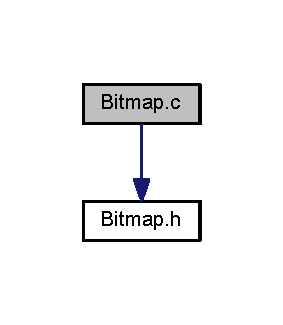
\includegraphics[width=136pt]{_bitmap_8c__incl}
\end{center}
\end{figure}
\subsection*{Functions}
\begin{DoxyCompactItemize}
\item 
\hyperlink{struct_bitmap}{Bitmap} $\ast$ \hyperlink{group___bitmap_ga3506880ffd407c36eb8aaddd2c1606d2}{load\+Bitmap} (const char $\ast$filename)
\begin{DoxyCompactList}\small\item\em Loads a bmp image. \end{DoxyCompactList}\item 
void \hyperlink{group___bitmap_ga18d05a1c671f4638bc63d37874efb9d4}{draw\+Bitmap} (\hyperlink{struct_bitmap}{Bitmap} $\ast$bmp, int x, int y, \hyperlink{group___bitmap_gacdfaca60ec19c0265bac2692d7982726}{Alignment} alignment)
\begin{DoxyCompactList}\small\item\em Draws an unscaled, unrotated bitmap at the given position. \end{DoxyCompactList}\item 
void \hyperlink{group___bitmap_ga08c1d4f4fff81df260d979ea8fc1aa61}{delete\+Bitmap} (\hyperlink{struct_bitmap}{Bitmap} $\ast$bmp)
\begin{DoxyCompactList}\small\item\em Destroys the given bitmap, freeing all resources used by it. \end{DoxyCompactList}\end{DoxyCompactItemize}

\hypertarget{_bitmap_8h}{}\section{Bitmap.\+h File Reference}
\label{_bitmap_8h}\index{Bitmap.\+h@{Bitmap.\+h}}
This graph shows which files directly or indirectly include this file\+:
\nopagebreak
\begin{figure}[H]
\begin{center}
\leavevmode
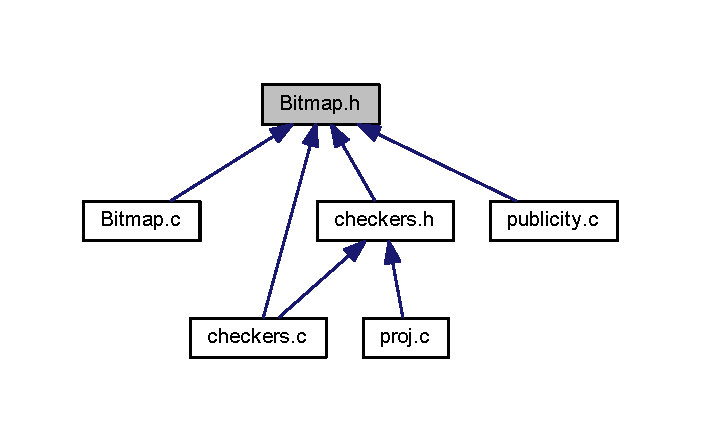
\includegraphics[width=337pt]{_bitmap_8h__dep__incl}
\end{center}
\end{figure}
\subsection*{Data Structures}
\begin{DoxyCompactItemize}
\item 
struct \hyperlink{struct_bitmap_file_header}{Bitmap\+File\+Header}
\item 
struct \hyperlink{struct_bitmap_info_header}{Bitmap\+Info\+Header}
\item 
struct \hyperlink{struct_bitmap}{Bitmap}
\end{DoxyCompactItemize}
\subsection*{Enumerations}
\begin{DoxyCompactItemize}
\item 
enum \hyperlink{group___bitmap_gacdfaca60ec19c0265bac2692d7982726}{Alignment} \{ \hyperlink{group___bitmap_ggacdfaca60ec19c0265bac2692d7982726a6ec599857e15466988726932dd592305}{A\+L\+I\+G\+N\+\_\+\+L\+E\+FT}, 
\hyperlink{group___bitmap_ggacdfaca60ec19c0265bac2692d7982726a5624165187e56db612253e608a45b1c6}{A\+L\+I\+G\+N\+\_\+\+C\+E\+N\+T\+ER}, 
\hyperlink{group___bitmap_ggacdfaca60ec19c0265bac2692d7982726a9c81840e8cad46418b39a8b74a246354}{A\+L\+I\+G\+N\+\_\+\+R\+I\+G\+HT}
 \}
\end{DoxyCompactItemize}
\subsection*{Functions}
\begin{DoxyCompactItemize}
\item 
\hyperlink{struct_bitmap}{Bitmap} $\ast$ \hyperlink{group___bitmap_ga3506880ffd407c36eb8aaddd2c1606d2}{load\+Bitmap} (const char $\ast$filename)
\begin{DoxyCompactList}\small\item\em Loads a bmp image. \end{DoxyCompactList}\item 
void \hyperlink{group___bitmap_ga18d05a1c671f4638bc63d37874efb9d4}{draw\+Bitmap} (\hyperlink{struct_bitmap}{Bitmap} $\ast$bitmap, int x, int y, \hyperlink{group___bitmap_gacdfaca60ec19c0265bac2692d7982726}{Alignment} alignment)
\begin{DoxyCompactList}\small\item\em Draws an unscaled, unrotated bitmap at the given position. \end{DoxyCompactList}\item 
void \hyperlink{group___bitmap_ga08c1d4f4fff81df260d979ea8fc1aa61}{delete\+Bitmap} (\hyperlink{struct_bitmap}{Bitmap} $\ast$bmp)
\begin{DoxyCompactList}\small\item\em Destroys the given bitmap, freeing all resources used by it. \end{DoxyCompactList}\end{DoxyCompactItemize}

\hypertarget{checkers_8c}{}\section{checkers.\+c File Reference}
\label{checkers_8c}\index{checkers.\+c@{checkers.\+c}}
{\ttfamily \#include $<$errno.\+h$>$}\newline
{\ttfamily \#include $<$minix/drivers.\+h$>$}\newline
{\ttfamily \#include $<$limits.\+h$>$}\newline
{\ttfamily \#include $<$string.\+h$>$}\newline
{\ttfamily \#include $<$stdlib.\+h$>$}\newline
{\ttfamily \#include $<$stdarg.\+h$>$}\newline
{\ttfamily \#include \char`\"{}checkers.\+h\char`\"{}}\newline
{\ttfamily \#include \char`\"{}Program\+Logic.\+h\char`\"{}}\newline
{\ttfamily \#include \char`\"{}video\+\_\+gr.\+h\char`\"{}}\newline
{\ttfamily \#include \char`\"{}vbe.\+h\char`\"{}}\newline
{\ttfamily \#include \char`\"{}i8042.\+h\char`\"{}}\newline
{\ttfamily \#include \char`\"{}i8254.\+h\char`\"{}}\newline
{\ttfamily \#include \char`\"{}utilities.\+h\char`\"{}}\newline
{\ttfamily \#include \char`\"{}mouse.\+h\char`\"{}}\newline
{\ttfamily \#include \char`\"{}timer.\+h\char`\"{}}\newline
{\ttfamily \#include \char`\"{}Bitmap.\+h\char`\"{}}\newline
{\ttfamily \#include \char`\"{}kbc.\+h\char`\"{}}\newline
{\ttfamily \#include \char`\"{}proj.\+h\char`\"{}}\newline
{\ttfamily \#include \char`\"{}publicity.\+h\char`\"{}}\newline
Include dependency graph for checkers.\+c\+:
\nopagebreak
\begin{figure}[H]
\begin{center}
\leavevmode
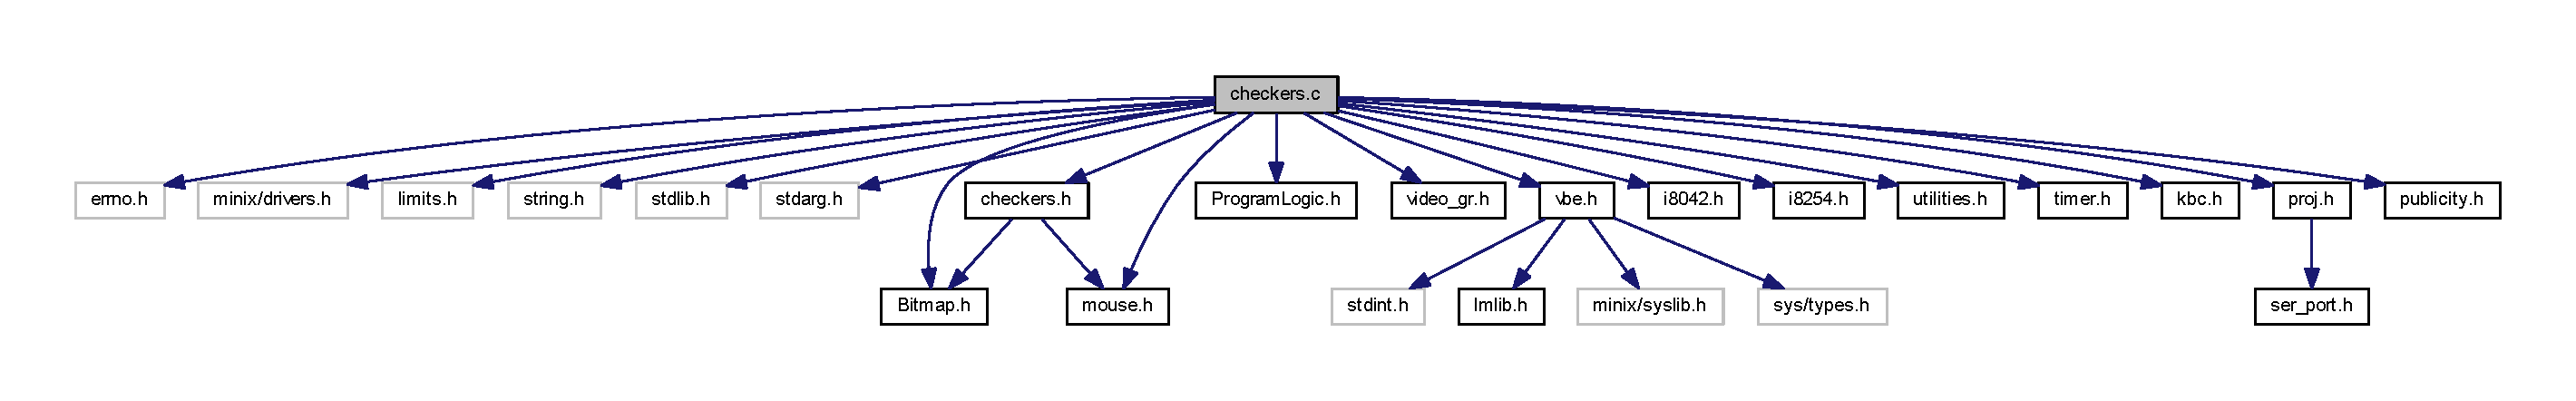
\includegraphics[width=350pt]{checkers_8c__incl}
\end{center}
\end{figure}
\subsection*{Functions}
\begin{DoxyCompactItemize}
\item 
int \hyperlink{group___checkers_gad95d8a331ab0758ace223ea301a57f7f}{checkers\+\_\+start\+\_\+game} (char $\ast$path\+\_\+images, int player\+\_\+1, int player\+\_\+2)
\begin{DoxyCompactList}\small\item\em loads the images and starts the game \end{DoxyCompactList}\item 
int \hyperlink{group___checkers_gaf1aa642150939b8b1d104fe437a9d135}{checkers\+\_\+serial\+\_\+handler} (int player1, int player2)
\begin{DoxyCompactList}\small\item\em handles the game in serial mode being responsible for handling which player should play \end{DoxyCompactList}\item 
int \hyperlink{group___checkers_ga61f35c6c9bba94dcd5028e185f3ae3f6}{checkers\+\_\+int\+\_\+handler} (int player1, int player2)
\begin{DoxyCompactList}\small\item\em handles the interrupts \end{DoxyCompactList}\item 
int \hyperlink{group___checkers_gac38396bd73b19b176b4016524f63f8aa}{checkers\+\_\+move\+\_\+handler} (\hyperlink{structmouse__packet__t}{mouse\+\_\+packet\+\_\+t} packet, int player1, int player2)
\begin{DoxyCompactList}\small\item\em handles the moves \end{DoxyCompactList}\item 
int \hyperlink{group___checkers_gac0cf60fd44a44bbb1a7c9ff7ec0d998b}{send\+\_\+serial\+\_\+move} (int player, int xi, int yi, int xf, int yf)
\begin{DoxyCompactList}\small\item\em Sends a message saying that a player did a move. \end{DoxyCompactList}\item 
int \hyperlink{group___checkers_gaa082b9cac17a99c54ac6fa5ac40c660d}{send\+\_\+serial\+\_\+ret} (int r)
\begin{DoxyCompactList}\small\item\em sends a serial message saying that a player finished making a move with the corresponding return value \end{DoxyCompactList}\item 
int \hyperlink{group___checkers_ga17180b891d06475062d87e08d01af278}{wait\+\_\+for\+\_\+serial\+\_\+message} (int player, int $\ast$r, int $\ast$xi, int $\ast$yi, int $\ast$xf, int $\ast$yf)
\begin{DoxyCompactList}\small\item\em Waits for a message from the serial port. \end{DoxyCompactList}\item 
int \hyperlink{group___checkers_gaa6a495a94944bda567df909f84c62396}{draw\+\_\+board} ()
\begin{DoxyCompactList}\small\item\em draws a board on the screen \end{DoxyCompactList}\item 
int \hyperlink{group___checkers_gaf3fd6677c55727d50220875a0031230b}{put\+\_\+square} (int board\+\_\+x, int board\+\_\+y, int color)
\begin{DoxyCompactList}\small\item\em places an empty square \end{DoxyCompactList}\item 
int \hyperlink{group___checkers_ga1d2d36062ce4e9fcdba43dfdc59215d0}{put\+\_\+circle} (int board\+\_\+x, int board\+\_\+y, int color)
\begin{DoxyCompactList}\small\item\em places a circle \end{DoxyCompactList}\item 
int \hyperlink{group___checkers_gaa0642fe5ef48cc14ab51722047092f1f}{move\+\_\+piece} (int player, int xi, int yi, int xf, int yf)
\begin{DoxyCompactList}\small\item\em moves a piece and handles everything pertinent related to the move \end{DoxyCompactList}\item 
int \hyperlink{group___checkers_ga01bdfba712e2ceab4902f5cd63f6b482}{draw\+\_\+turn\+\_\+message} (int x, int y, unsigned int background\+\_\+clr, \hyperlink{struct_bitmap}{Bitmap} $\ast$turn)
\begin{DoxyCompactList}\small\item\em draws the turn message that says who should play now \end{DoxyCompactList}\item 
int \hyperlink{group___checkers_gae4a0f98e772d41a53d13748a7d9d1252}{coord\+\_\+to\+\_\+real\+\_\+board} (int coord\+\_\+x, int coord\+\_\+y, int $\ast$board\+\_\+x, int $\ast$board\+\_\+y)
\begin{DoxyCompactList}\small\item\em converts screen coordinates to board coordinates \end{DoxyCompactList}\item 
int \hyperlink{group___checkers_gad7f7feb83c536c88d67834e7e20780ee}{state\+\_\+to\+\_\+player} (int \hyperlink{checkers_8c_a89f234133d3efe315836311cbf21c64b}{state})
\begin{DoxyCompactList}\small\item\em converts a state to the corresponding player \end{DoxyCompactList}\item 
int \hyperlink{group___checkers_ga258c52e2e4a6ef24d9fb5ec06bedaa53}{create\+\_\+mouse} (int x, int y)
\item 
int \hyperlink{group___checkers_ga597f43aacf586aacf3c32664944f8ba9}{move\+\_\+mouse} (int x\+\_\+delta, int y\+\_\+delta)
\begin{DoxyCompactList}\small\item\em moves mouse (x\+\_\+delta, y\+\_\+delta) \end{DoxyCompactList}\item 
int \hyperlink{group___checkers_ga0f9d87b0bea416d794ed80855026d550}{draw\+\_\+mouse} ()
\begin{DoxyCompactList}\small\item\em draws a mouse \end{DoxyCompactList}\item 
int \hyperlink{group___checkers_ga0580c6365cfa09e2d8a30d3d47f3adb1}{draw\+\_\+mouse\+\_\+circle} (int xi, int yi, int radius, int color)
\begin{DoxyCompactList}\small\item\em draws the the mouse circle \end{DoxyCompactList}\item 
int \hyperlink{checkers_8c_aacaf4b2a6f8825bb15f2b4a372974cce}{delete\+\_\+mouse} ()
\end{DoxyCompactItemize}
\subsection*{Variables}
\begin{DoxyCompactItemize}
\item 
static int \hyperlink{checkers_8c_a89f234133d3efe315836311cbf21c64b}{state} =\hyperlink{group___checkers_gga06fc87d81c62e9abb8790b6e5713c55bad88d91bd9763e878df21645bae0ba9b5}{S\+T\+A\+T\+E\+\_\+1\+\_\+\+D\+E\+F\+A\+U\+LT}
\item 
static char \hyperlink{checkers_8c_a12f50bd537a3a737da9d47710c308ae3}{board} \mbox{[}8\mbox{]}\mbox{[}8\mbox{]}
\item 
static \hyperlink{structmouse__t}{mouse\+\_\+t} $\ast$ \hyperlink{checkers_8c_ab4e895b3d4aa209fc0ffc3adeffebb33}{mouse}
\item 
static \hyperlink{struct_bitmap}{Bitmap} $\ast$ \hyperlink{checkers_8c_acd442af53aa26eaeef242c9483ee06b9}{cursor}
\item 
static \hyperlink{struct_bitmap}{Bitmap} $\ast$ \hyperlink{checkers_8c_a6be9c164fb2985f9dcdcdcbae6673ac1}{redturn}
\item 
static \hyperlink{struct_bitmap}{Bitmap} $\ast$ \hyperlink{checkers_8c_ae52b102643b34da7b84294f2812902cb}{yellowturn}
\item 
static \hyperlink{struct_bitmap}{Bitmap} $\ast$ \hyperlink{checkers_8c_a15de70574bc710486bf129a5c8f1634e}{background}
\end{DoxyCompactItemize}


\subsection{Function Documentation}
\hypertarget{checkers_8c_aacaf4b2a6f8825bb15f2b4a372974cce}{}\label{checkers_8c_aacaf4b2a6f8825bb15f2b4a372974cce} 
\index{checkers.\+c@{checkers.\+c}!delete\+\_\+mouse@{delete\+\_\+mouse}}
\index{delete\+\_\+mouse@{delete\+\_\+mouse}!checkers.\+c@{checkers.\+c}}
\subsubsection{\texorpdfstring{delete\+\_\+mouse()}{delete\_mouse()}}
{\footnotesize\ttfamily int delete\+\_\+mouse (\begin{DoxyParamCaption}{ }\end{DoxyParamCaption})}



\subsection{Variable Documentation}
\hypertarget{checkers_8c_a15de70574bc710486bf129a5c8f1634e}{}\label{checkers_8c_a15de70574bc710486bf129a5c8f1634e} 
\index{checkers.\+c@{checkers.\+c}!background@{background}}
\index{background@{background}!checkers.\+c@{checkers.\+c}}
\subsubsection{\texorpdfstring{background}{background}}
{\footnotesize\ttfamily \hyperlink{struct_bitmap}{Bitmap}$\ast$ background\hspace{0.3cm}{\ttfamily [static]}}

\hypertarget{checkers_8c_a12f50bd537a3a737da9d47710c308ae3}{}\label{checkers_8c_a12f50bd537a3a737da9d47710c308ae3} 
\index{checkers.\+c@{checkers.\+c}!board@{board}}
\index{board@{board}!checkers.\+c@{checkers.\+c}}
\subsubsection{\texorpdfstring{board}{board}}
{\footnotesize\ttfamily char board\mbox{[}8\mbox{]}\mbox{[}8\mbox{]}\hspace{0.3cm}{\ttfamily [static]}}

\hypertarget{checkers_8c_acd442af53aa26eaeef242c9483ee06b9}{}\label{checkers_8c_acd442af53aa26eaeef242c9483ee06b9} 
\index{checkers.\+c@{checkers.\+c}!cursor@{cursor}}
\index{cursor@{cursor}!checkers.\+c@{checkers.\+c}}
\subsubsection{\texorpdfstring{cursor}{cursor}}
{\footnotesize\ttfamily \hyperlink{struct_bitmap}{Bitmap}$\ast$ cursor\hspace{0.3cm}{\ttfamily [static]}}

\hypertarget{checkers_8c_ab4e895b3d4aa209fc0ffc3adeffebb33}{}\label{checkers_8c_ab4e895b3d4aa209fc0ffc3adeffebb33} 
\index{checkers.\+c@{checkers.\+c}!mouse@{mouse}}
\index{mouse@{mouse}!checkers.\+c@{checkers.\+c}}
\subsubsection{\texorpdfstring{mouse}{mouse}}
{\footnotesize\ttfamily \hyperlink{structmouse__t}{mouse\+\_\+t}$\ast$ mouse\hspace{0.3cm}{\ttfamily [static]}}

\hypertarget{checkers_8c_a6be9c164fb2985f9dcdcdcbae6673ac1}{}\label{checkers_8c_a6be9c164fb2985f9dcdcdcbae6673ac1} 
\index{checkers.\+c@{checkers.\+c}!redturn@{redturn}}
\index{redturn@{redturn}!checkers.\+c@{checkers.\+c}}
\subsubsection{\texorpdfstring{redturn}{redturn}}
{\footnotesize\ttfamily \hyperlink{struct_bitmap}{Bitmap}$\ast$ redturn\hspace{0.3cm}{\ttfamily [static]}}

\hypertarget{checkers_8c_a89f234133d3efe315836311cbf21c64b}{}\label{checkers_8c_a89f234133d3efe315836311cbf21c64b} 
\index{checkers.\+c@{checkers.\+c}!state@{state}}
\index{state@{state}!checkers.\+c@{checkers.\+c}}
\subsubsection{\texorpdfstring{state}{state}}
{\footnotesize\ttfamily int state =\hyperlink{group___checkers_gga06fc87d81c62e9abb8790b6e5713c55bad88d91bd9763e878df21645bae0ba9b5}{S\+T\+A\+T\+E\+\_\+1\+\_\+\+D\+E\+F\+A\+U\+LT}\hspace{0.3cm}{\ttfamily [static]}}

\hypertarget{checkers_8c_ae52b102643b34da7b84294f2812902cb}{}\label{checkers_8c_ae52b102643b34da7b84294f2812902cb} 
\index{checkers.\+c@{checkers.\+c}!yellowturn@{yellowturn}}
\index{yellowturn@{yellowturn}!checkers.\+c@{checkers.\+c}}
\subsubsection{\texorpdfstring{yellowturn}{yellowturn}}
{\footnotesize\ttfamily \hyperlink{struct_bitmap}{Bitmap}$\ast$ yellowturn\hspace{0.3cm}{\ttfamily [static]}}


\hypertarget{checkers_8h}{}\section{checkers.\+h File Reference}
\label{checkers_8h}\index{checkers.\+h@{checkers.\+h}}
{\ttfamily \#include \char`\"{}Bitmap.\+h\char`\"{}}\newline
{\ttfamily \#include \char`\"{}mouse.\+h\char`\"{}}\newline
Include dependency graph for checkers.\+h\+:
\nopagebreak
\begin{figure}[H]
\begin{center}
\leavevmode
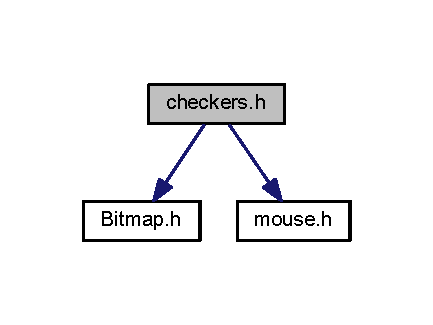
\includegraphics[width=208pt]{checkers_8h__incl}
\end{center}
\end{figure}
This graph shows which files directly or indirectly include this file\+:
\nopagebreak
\begin{figure}[H]
\begin{center}
\leavevmode
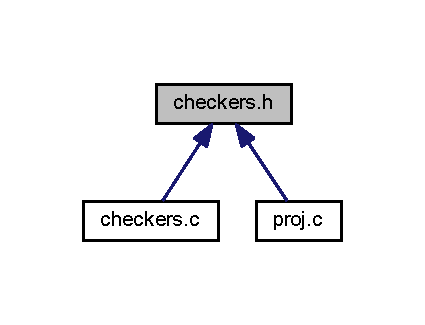
\includegraphics[width=204pt]{checkers_8h__dep__incl}
\end{center}
\end{figure}
\subsection*{Data Structures}
\begin{DoxyCompactItemize}
\item 
struct \hyperlink{structmouse__t}{mouse\+\_\+t}
\end{DoxyCompactItemize}
\subsection*{Macros}
\begin{DoxyCompactItemize}
\item 
\#define \hyperlink{group___checkers_ga2f705e070c4925daee2fda4016de437f}{C\+H\+E\+C\+K\+E\+R\+S\+\_\+\+T\+I\+M\+E\+O\+UT}~30
\item 
\#define \hyperlink{group___checkers_ga455c619153ef283f338157e6b2156179}{W\+H\+I\+T\+E\+\_\+\+C\+LR}~0x\+F\+F\+FF
\item 
\#define \hyperlink{group___checkers_ga84d1df2a2deef34e0e9f8d4375b5b8f6}{B\+L\+A\+C\+K\+\_\+\+C\+LR}~0
\item 
\#define \hyperlink{group___checkers_gaaf27b1edff1c7d7a5bf0a59ecb27cb5d}{B\+O\+A\+R\+D\+\_\+\+XI}~320
\item 
\#define \hyperlink{group___checkers_gaea13da4098bc5828bb6b3f6febcfd904}{B\+O\+A\+R\+D\+\_\+\+YI}~192
\item 
\#define \hyperlink{group___checkers_gae49255d26a5f626f705a0ab09f3f2fb8}{B\+O\+A\+R\+D\+\_\+\+S\+Q\+\_\+\+S\+I\+ZE}~80
\item 
\#define \hyperlink{group___checkers_ga0db4eef7cbfb2b192b09094169ce388f}{B\+O\+A\+R\+D\+\_\+\+C\+L\+\_\+\+R\+A\+D\+I\+US}~32
\item 
\#define \hyperlink{group___checkers_ga63f26b52fc35e2f57f2212dd1478d076}{B\+O\+A\+R\+D\+\_\+\+E\+V\+E\+N\+\_\+\+S\+Q\+\_\+\+C\+LR}~0x\+C618
\item 
\#define \hyperlink{group___checkers_ga07198a5ebf1a6ac88de94970f135a8ba}{B\+O\+A\+R\+D\+\_\+\+O\+D\+D\+\_\+\+S\+Q\+\_\+\+C\+LR}~0x18\+C9
\item 
\#define \hyperlink{group___checkers_ga0d38fb3c6c1987840ddb97f7696d997d}{B\+O\+A\+R\+D\+\_\+\+P\+L1\+\_\+\+C\+L\+\_\+\+C\+LR}~0x\+E\+E\+C4
\begin{DoxyCompactList}\small\item\em E8\+D820. \end{DoxyCompactList}\item 
\#define \hyperlink{group___checkers_gaf7041b1453aa70a12d1dac1602d93ca8}{B\+O\+A\+R\+D\+\_\+\+P\+L2\+\_\+\+C\+L\+\_\+\+C\+LR}~0x\+C945
\begin{DoxyCompactList}\small\item\em C82828. \end{DoxyCompactList}\item 
\#define \hyperlink{group___checkers_gaab1a3cc5eb6c2a45aca8a4d8a5e08707}{M\+O\+U\+S\+E\+\_\+\+T\+R\+A\+N\+S\+P\+A\+R\+E\+N\+T\+\_\+\+C\+LR}~0x\+F81F
\item 
\#define \hyperlink{group___checkers_gaa2ef662fb61ca6849a43030a495c4afa}{M\+O\+U\+S\+E\+\_\+\+T\+R\+A\+N\+S\+P\+A\+R\+E\+N\+T\+\_\+\+C\+L\+R\+\_\+2}~0x0001
\item 
\#define \hyperlink{group___checkers_gac55bb8c3d7fd471107553465b14fae49}{T\+U\+R\+N\+\_\+\+M\+S\+G\+\_\+\+C\+LR}~0x1383
\item 
\#define \hyperlink{group___checkers_ga6d237f394788ef28deeaf21d0a6637f2}{T\+U\+R\+N\+\_\+\+M\+S\+G\+\_\+\+Y\+E\+L\+L\+O\+W\+\_\+\+B\+A\+C\+K\+G\+R\+O\+U\+N\+D\+\_\+\+C\+LR}~0x\+E6\+A5
\item 
\#define \hyperlink{group___checkers_ga98c171a878c38e1c25fb081562041c44}{T\+U\+R\+N\+\_\+\+M\+S\+G\+\_\+\+R\+E\+D\+\_\+\+B\+A\+C\+K\+G\+R\+O\+U\+N\+D\+\_\+\+C\+LR}~0x\+C146
\item 
\#define \hyperlink{group___checkers_gaf92e8ff13dda8277eaf67d6a59863510}{T\+U\+R\+N\+\_\+\+M\+S\+G\+\_\+\+X\+I\+\_\+\+R\+ED}~540
\item 
\#define \hyperlink{group___checkers_gae8d1a563a8d7003deca2e08f762ae9f7}{T\+U\+R\+N\+\_\+\+M\+S\+G\+\_\+\+X\+I\+\_\+\+Y\+E\+L\+L\+OW}~480
\item 
\#define \hyperlink{group___checkers_gad96cfcfb473995338b12290370836079}{T\+U\+R\+N\+\_\+\+M\+S\+G\+\_\+\+YI}~100
\end{DoxyCompactItemize}
\subsection*{Enumerations}
\begin{DoxyCompactItemize}
\item 
enum \{ \hyperlink{group___checkers_gga06fc87d81c62e9abb8790b6e5713c55bacad03968ad3abc8b7121ad472826aca9}{S\+T\+A\+T\+E\+\_\+1\+\_\+\+H\+O\+L\+D\+\_\+\+P\+I\+E\+CE}, 
\hyperlink{group___checkers_gga06fc87d81c62e9abb8790b6e5713c55bad88d91bd9763e878df21645bae0ba9b5}{S\+T\+A\+T\+E\+\_\+1\+\_\+\+D\+E\+F\+A\+U\+LT}, 
\hyperlink{group___checkers_gga06fc87d81c62e9abb8790b6e5713c55ba946a863b3f5d8ac63feb55f4e0866597}{S\+T\+A\+T\+E\+\_\+2\+\_\+\+H\+O\+L\+D\+\_\+\+P\+I\+E\+CE}, 
\hyperlink{group___checkers_gga06fc87d81c62e9abb8790b6e5713c55ba156b7cbfed5b8a1ad54b568ebc257ae9}{S\+T\+A\+T\+E\+\_\+2\+\_\+\+D\+E\+F\+A\+U\+LT}
 \}
\end{DoxyCompactItemize}
\subsection*{Functions}
\begin{DoxyCompactItemize}
\item 
int \hyperlink{group___checkers_gad95d8a331ab0758ace223ea301a57f7f}{checkers\+\_\+start\+\_\+game} (char $\ast$path\+\_\+images, int player\+\_\+1, int player\+\_\+2)
\begin{DoxyCompactList}\small\item\em loads the images and starts the game \end{DoxyCompactList}\item 
int \hyperlink{group___checkers_gaf1aa642150939b8b1d104fe437a9d135}{checkers\+\_\+serial\+\_\+handler} (int player\+\_\+1, int player\+\_\+2)
\begin{DoxyCompactList}\small\item\em handles the game in serial mode being responsible for handling which player should play \end{DoxyCompactList}\item 
int \hyperlink{group___checkers_ga61f35c6c9bba94dcd5028e185f3ae3f6}{checkers\+\_\+int\+\_\+handler} (int player1, int player2)
\begin{DoxyCompactList}\small\item\em handles the interrupts \end{DoxyCompactList}\item 
int \hyperlink{group___checkers_gac38396bd73b19b176b4016524f63f8aa}{checkers\+\_\+move\+\_\+handler} (\hyperlink{structmouse__packet__t}{mouse\+\_\+packet\+\_\+t} packet, int player1, int player2)
\begin{DoxyCompactList}\small\item\em handles the moves \end{DoxyCompactList}\item 
int \hyperlink{group___checkers_gac0cf60fd44a44bbb1a7c9ff7ec0d998b}{send\+\_\+serial\+\_\+move} (int player, int xi, int yi, int xf, int yf)
\begin{DoxyCompactList}\small\item\em Sends a message saying that a player did a move. \end{DoxyCompactList}\item 
int \hyperlink{group___checkers_gaa082b9cac17a99c54ac6fa5ac40c660d}{send\+\_\+serial\+\_\+ret} (int r)
\begin{DoxyCompactList}\small\item\em sends a serial message saying that a player finished making a move with the corresponding return value \end{DoxyCompactList}\item 
int \hyperlink{group___checkers_ga17180b891d06475062d87e08d01af278}{wait\+\_\+for\+\_\+serial\+\_\+message} (int player, int $\ast$r, int $\ast$xi, int $\ast$yi, int $\ast$xf, int $\ast$yf)
\begin{DoxyCompactList}\small\item\em Waits for a message from the serial port. \end{DoxyCompactList}\item 
int \hyperlink{group___checkers_gaa6a495a94944bda567df909f84c62396}{draw\+\_\+board} ()
\begin{DoxyCompactList}\small\item\em draws a board on the screen \end{DoxyCompactList}\item 
int \hyperlink{group___checkers_gaf3fd6677c55727d50220875a0031230b}{put\+\_\+square} (int board\+\_\+x, int board\+\_\+y, int color)
\begin{DoxyCompactList}\small\item\em places an empty square \end{DoxyCompactList}\item 
int \hyperlink{group___checkers_ga1d2d36062ce4e9fcdba43dfdc59215d0}{put\+\_\+circle} (int board\+\_\+x, int board\+\_\+y, int color)
\begin{DoxyCompactList}\small\item\em places a circle \end{DoxyCompactList}\item 
int \hyperlink{group___checkers_gaa0642fe5ef48cc14ab51722047092f1f}{move\+\_\+piece} (int player, int xi, int yi, int xf, int yf)
\begin{DoxyCompactList}\small\item\em moves a piece and handles everything pertinent related to the move \end{DoxyCompactList}\item 
int \hyperlink{group___checkers_ga01bdfba712e2ceab4902f5cd63f6b482}{draw\+\_\+turn\+\_\+message} (int x, int y, unsigned int background\+\_\+clr, \hyperlink{struct_bitmap}{Bitmap} $\ast$turn)
\begin{DoxyCompactList}\small\item\em draws the turn message that says who should play now \end{DoxyCompactList}\item 
int \hyperlink{group___checkers_gae4a0f98e772d41a53d13748a7d9d1252}{coord\+\_\+to\+\_\+real\+\_\+board} (int coord\+\_\+x, int coord\+\_\+y, int $\ast$board\+\_\+x, int $\ast$board\+\_\+y)
\begin{DoxyCompactList}\small\item\em converts screen coordinates to board coordinates \end{DoxyCompactList}\item 
int \hyperlink{group___checkers_gad7f7feb83c536c88d67834e7e20780ee}{state\+\_\+to\+\_\+player} (int \hyperlink{checkers_8c_a89f234133d3efe315836311cbf21c64b}{state})
\begin{DoxyCompactList}\small\item\em converts a state to the corresponding player \end{DoxyCompactList}\item 
int \hyperlink{group___checkers_ga258c52e2e4a6ef24d9fb5ec06bedaa53}{create\+\_\+mouse} (int x, int y)
\item 
int \hyperlink{group___checkers_ga597f43aacf586aacf3c32664944f8ba9}{move\+\_\+mouse} (int x\+\_\+delta, int y\+\_\+delta)
\begin{DoxyCompactList}\small\item\em moves mouse (x\+\_\+delta, y\+\_\+delta) \end{DoxyCompactList}\item 
int \hyperlink{group___checkers_ga0f9d87b0bea416d794ed80855026d550}{draw\+\_\+mouse} ()
\begin{DoxyCompactList}\small\item\em draws a mouse \end{DoxyCompactList}\item 
int \hyperlink{group___checkers_ga0580c6365cfa09e2d8a30d3d47f3adb1}{draw\+\_\+mouse\+\_\+circle} (int xi, int yi, int radius, int color)
\begin{DoxyCompactList}\small\item\em draws the the mouse circle \end{DoxyCompactList}\end{DoxyCompactItemize}

\hypertarget{i8042_8h}{}\section{i8042.\+h File Reference}
\label{i8042_8h}\index{i8042.\+h@{i8042.\+h}}
This graph shows which files directly or indirectly include this file\+:
\nopagebreak
\begin{figure}[H]
\begin{center}
\leavevmode
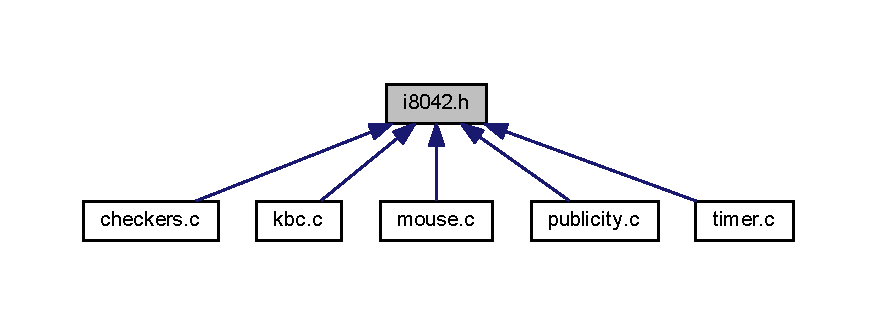
\includegraphics[width=350pt]{i8042_8h__dep__incl}
\end{center}
\end{figure}
\subsection*{Macros}
\begin{Indent}{\bf K\+BC}\par
\begin{DoxyCompactItemize}
\item 
\#define \hyperlink{group__i8042_ga16c5827f043d82f87c726c2d4369c11d}{K\+B\+C\+\_\+\+I\+RQ}~1
\item 
\#define \hyperlink{group__i8042_ga1ccde68b2b6d4e45b50eef1403e10bb7}{K\+B\+C\+\_\+\+O\+U\+T\+\_\+\+B\+UF}~0x60
\item 
\#define \hyperlink{group__i8042_gaac9289c99cf0a693a211da6d6cb1bb65}{K\+B\+C\+\_\+\+I\+N\+\_\+\+B\+UF}~0x60
\item 
\#define \hyperlink{group__i8042_ga34b14687d83496940a236351fbbb1aea}{K\+B\+C\+\_\+\+S\+T\+A\+T\+\_\+\+R\+EG}~0x64
\item 
\#define \hyperlink{group__i8042_ga6d57c7927a10f638c83046b52c8caac9}{K\+B\+C\+\_\+\+C\+M\+D\+\_\+\+R\+EG}~0x64
\item 
\#define \hyperlink{group__i8042_ga7bff22c3c71947a24f8f0922d33f0f5f}{C\+K\+B\+D\+\_\+\+A\+CK}~0xfa
\item 
\#define \hyperlink{group__i8042_gafbc8d3dd7a27e8c020c9991578358def}{C\+K\+B\+D\+\_\+\+R\+E\+S\+E\+ND}~0xfe
\item 
\#define \hyperlink{group__i8042_ga318cf5bf776792ffc02a53fb7e8082df}{C\+K\+B\+D\+\_\+\+E\+R\+R\+OR}~0xfc
\item 
\#define \hyperlink{group__i8042_ga36930de8a703505c95fe133095dcfe06}{K\+B\+C\+\_\+\+O\+BF}~\hyperlink{video__gr_8c_a3a8ea58898cb58fc96013383d39f482c}{B\+IT}(0)
\item 
\#define \hyperlink{group__i8042_gac1649d41f8ba9a02fa70ec4e600d5e4a}{K\+B\+C\+\_\+\+I\+BF}~\hyperlink{video__gr_8c_a3a8ea58898cb58fc96013383d39f482c}{B\+IT}(1)
\item 
\#define \hyperlink{group__i8042_ga795488c410d300a8ea2afb4c82d2e6cc}{K\+B\+C\+\_\+\+P\+A\+R\+\_\+\+E\+R\+R\+OR}~\hyperlink{video__gr_8c_a3a8ea58898cb58fc96013383d39f482c}{B\+IT}(7)
\item 
\#define \hyperlink{group__i8042_ga22767b69efd74d1f3631b8803a63b939}{K\+B\+C\+\_\+\+T\+O\+\_\+\+E\+R\+R\+OR}~\hyperlink{video__gr_8c_a3a8ea58898cb58fc96013383d39f482c}{B\+IT}(6)
\item 
\#define \hyperlink{group__i8042_ga1747d582dc5a6d634f05016ece9625d8}{K\+B\+C\+\_\+\+W\+R\+I\+T\+E\+\_\+\+T\+O\+\_\+\+M\+O\+U\+SE}~0x\+D4
\item 
\#define \hyperlink{group__i8042_gac69c14ded6b68de11e5caaa6bcddf8fc}{K\+B\+D\+\_\+\+L\+E\+DS}~0xed
\item 
\#define \hyperlink{group__i8042_ga1b7a8d18cf6c99a32610259ae861eb1f}{K\+B\+D\+\_\+\+L\+ED}(n)~(1$<$$<$n)
\end{DoxyCompactItemize}
\end{Indent}
\begin{Indent}{\bf M\+O\+U\+SE}\par
\begin{DoxyCompactItemize}
\item 
\#define \hyperlink{group__i8042_ga85964cb90343bb1a029b1d1b4229f910}{M\+O\+U\+S\+E\+\_\+\+I\+RQ}~12
\item 
\#define \hyperlink{group__i8042_ga6b902000c4f0a66e57f0eb78d7611105}{M\+O\+U\+S\+E\+\_\+\+R\+E\+S\+ET}~0xff
\item 
\#define \hyperlink{group__i8042_ga094907f521b569f790a760be8885ec4d}{M\+O\+U\+S\+E\+\_\+\+D\+I\+S\+A\+B\+LE}~0xf5
\item 
\#define \hyperlink{group__i8042_ga4e6aa8d10e05b5f94c196bfe2cdfb8d7}{M\+O\+U\+S\+E\+\_\+\+E\+N\+A\+B\+LE}~0xf4
\item 
\#define \hyperlink{group__i8042_gafcda52e19d0d6e3053ec9e51c548254d}{M\+O\+U\+S\+E\+\_\+\+S\+E\+T\+\_\+\+S\+T\+R\+E\+AM}~0xea
\item 
\#define \hyperlink{group__i8042_gadb427fdde0b4b8715e843c54e1ae7522}{M\+O\+U\+S\+E\+\_\+\+D\+I\+S\+A\+B\+L\+E\+\_\+\+S\+T\+R\+E\+A\+M\+\_\+\+M\+O\+DE}~0\+X\+F5
\item 
\#define \hyperlink{group__i8042_gae81dac725cb48935cbc4564c35a46c5d}{M\+O\+U\+S\+E\+\_\+\+S\+T\+A\+T\+U\+S\+\_\+\+R\+E\+Q\+U\+E\+ST}~0x\+E9
\end{DoxyCompactItemize}
\end{Indent}

\hypertarget{i8254_8h}{}\section{i8254.\+h File Reference}
\label{i8254_8h}\index{i8254.\+h@{i8254.\+h}}
This graph shows which files directly or indirectly include this file\+:
\nopagebreak
\begin{figure}[H]
\begin{center}
\leavevmode
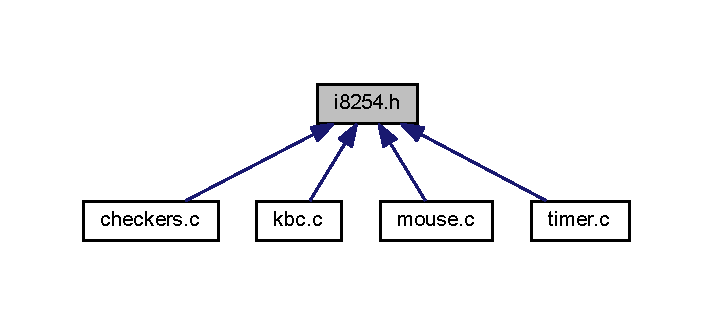
\includegraphics[width=342pt]{i8254_8h__dep__incl}
\end{center}
\end{figure}
\subsection*{Macros}
\begin{DoxyCompactItemize}
\item 
\#define \hyperlink{group__i8254_gacf926951944b6cf370b7229ebd50dd8b}{T\+I\+M\+E\+R\+\_\+\+F\+R\+EQ}~1193182
\begin{DoxyCompactList}\small\item\em clock frequency for timer in PC and AT \end{DoxyCompactList}\item 
\#define \hyperlink{group__i8254_ga30bf84c312af248cb81bb224e09f9ba8}{T\+I\+M\+E\+R0\+\_\+\+I\+RQ}~0
\begin{DoxyCompactList}\small\item\em Timer 0 I\+RQ line. \end{DoxyCompactList}\end{DoxyCompactItemize}
\begin{Indent}{\bf I/O port addresses}\par
\begin{DoxyCompactItemize}
\item 
\#define \hyperlink{group__i8254_gacc9ff9df4a9674a1ce9ba08fc4a4679e}{T\+I\+M\+E\+R\+\_\+0}~0x40
\begin{DoxyCompactList}\small\item\em Timer 0 count register. \end{DoxyCompactList}\item 
\#define \hyperlink{group__i8254_gac62c99c2a9289891c1b83052242cca49}{T\+I\+M\+E\+R\+\_\+1}~0x41
\begin{DoxyCompactList}\small\item\em Timer 1 count register. \end{DoxyCompactList}\item 
\#define \hyperlink{group__i8254_ga1f34f18ad0ab8cace46b615773b48735}{T\+I\+M\+E\+R\+\_\+2}~0x42
\begin{DoxyCompactList}\small\item\em Timer 2 count register. \end{DoxyCompactList}\item 
\#define \hyperlink{group__i8254_ga282832448fb0281ef53d243c1cd48491}{T\+I\+M\+E\+R\+\_\+\+C\+T\+RL}~0x43
\begin{DoxyCompactList}\small\item\em Control register. \end{DoxyCompactList}\item 
\#define \hyperlink{group__i8254_ga51b3a5e3d4811ca063fe25e35560ab40}{S\+P\+E\+A\+K\+E\+R\+\_\+\+C\+T\+RL}~0x61
\begin{DoxyCompactList}\small\item\em Register for speaker control. \end{DoxyCompactList}\end{DoxyCompactItemize}
\end{Indent}
\begin{Indent}{\bf Timer selection\+: bits 7 and 6}\par
\begin{DoxyCompactItemize}
\item 
\#define \hyperlink{group__i8254_ga6a4822642d40c248435692324a818010}{T\+I\+M\+E\+R\+\_\+\+S\+E\+L0}~0x00
\begin{DoxyCompactList}\small\item\em Control Word for Timer 0. \end{DoxyCompactList}\item 
\#define \hyperlink{group__i8254_ga8349623fd8d99f9cc5d8ae29d78594fc}{T\+I\+M\+E\+R\+\_\+\+S\+E\+L1}~\hyperlink{video__gr_8c_a3a8ea58898cb58fc96013383d39f482c}{B\+IT}(6)
\begin{DoxyCompactList}\small\item\em Control Word for Timer 1. \end{DoxyCompactList}\item 
\#define \hyperlink{group__i8254_ga142a255de0dbc48aeabd45fc10c33672}{T\+I\+M\+E\+R\+\_\+\+S\+E\+L2}~\hyperlink{video__gr_8c_a3a8ea58898cb58fc96013383d39f482c}{B\+IT}(7)
\begin{DoxyCompactList}\small\item\em Control Word for Timer 2. \end{DoxyCompactList}\item 
\#define \hyperlink{group__i8254_ga4c2eecbfb96744a9c2af71dba75ecb18}{T\+I\+M\+E\+R\+\_\+\+R\+B\+\_\+\+C\+MD}~(\hyperlink{video__gr_8c_a3a8ea58898cb58fc96013383d39f482c}{B\+IT}(7)$\vert$\hyperlink{video__gr_8c_a3a8ea58898cb58fc96013383d39f482c}{B\+IT}(6))
\begin{DoxyCompactList}\small\item\em Read Back Command. \end{DoxyCompactList}\end{DoxyCompactItemize}
\end{Indent}
\begin{Indent}{\bf Register selection\+: bits 5 and 4}\par
\begin{DoxyCompactItemize}
\item 
\#define \hyperlink{group__i8254_gac18cb814ebd0d67235392c330e0e3504}{T\+I\+M\+E\+R\+\_\+\+L\+SB}~\hyperlink{video__gr_8c_a3a8ea58898cb58fc96013383d39f482c}{B\+IT}(4)
\begin{DoxyCompactList}\small\item\em Initialize Counter L\+SB only. \end{DoxyCompactList}\item 
\#define \hyperlink{group__i8254_ga2a8a6d363c612d756cd8d78480f7cd04}{T\+I\+M\+E\+R\+\_\+\+M\+SB}~\hyperlink{video__gr_8c_a3a8ea58898cb58fc96013383d39f482c}{B\+IT}(5)
\begin{DoxyCompactList}\small\item\em Initialize Counter M\+SB only. \end{DoxyCompactList}\item 
\#define \hyperlink{group__i8254_ga8c0f1933323274c765e23837e4fbc8c7}{T\+I\+M\+E\+R\+\_\+\+L\+S\+B\+\_\+\+M\+SB}~(\hyperlink{group__i8254_gac18cb814ebd0d67235392c330e0e3504}{T\+I\+M\+E\+R\+\_\+\+L\+SB} $\vert$ \hyperlink{group__i8254_ga2a8a6d363c612d756cd8d78480f7cd04}{T\+I\+M\+E\+R\+\_\+\+M\+SB})
\begin{DoxyCompactList}\small\item\em Initialize L\+SB first and M\+SB afterwards. \end{DoxyCompactList}\end{DoxyCompactItemize}
\end{Indent}
\begin{Indent}{\bf Operating mode\+: bits 3, 2 and 1}\par
\begin{DoxyCompactItemize}
\item 
\#define \hyperlink{group__i8254_ga4745cbf21da3d3fea5dbb080b2b73bac}{T\+I\+M\+E\+R\+\_\+\+S\+Q\+R\+\_\+\+W\+A\+VE}~(\hyperlink{video__gr_8c_a3a8ea58898cb58fc96013383d39f482c}{B\+IT}(2)$\vert$\hyperlink{video__gr_8c_a3a8ea58898cb58fc96013383d39f482c}{B\+IT}(1))
\begin{DoxyCompactList}\small\item\em Mode 3\+: square wave generator. \end{DoxyCompactList}\item 
\#define \hyperlink{group__i8254_ga5d4449e0fa1cf4a4d107a48a04a1265f}{T\+I\+M\+E\+R\+\_\+\+R\+A\+T\+E\+\_\+\+G\+EN}~\hyperlink{video__gr_8c_a3a8ea58898cb58fc96013383d39f482c}{B\+IT}(2)
\begin{DoxyCompactList}\small\item\em Mode 2\+: rate generator. \end{DoxyCompactList}\end{DoxyCompactItemize}
\end{Indent}
\begin{Indent}{\bf Counting mode\+: bit 0}\par
\begin{DoxyCompactItemize}
\item 
\#define \hyperlink{group__i8254_ga325b992a371d5d981c4eceff42fa5956}{T\+I\+M\+E\+R\+\_\+\+B\+CD}~0x01
\begin{DoxyCompactList}\small\item\em Count in B\+CD. \end{DoxyCompactList}\item 
\#define \hyperlink{group__i8254_gad2913dcf2f91453317bd035589ac0a7d}{T\+I\+M\+E\+R\+\_\+\+B\+IN}~0x00
\begin{DoxyCompactList}\small\item\em Count in binary. \end{DoxyCompactList}\end{DoxyCompactItemize}
\end{Indent}
\begin{Indent}{\bf R\+E\+A\+D-\/\+B\+A\+CK C\+O\+M\+M\+A\+ND F\+O\+R\+M\+AT}\par
\begin{DoxyCompactItemize}
\item 
\#define \hyperlink{i8254_8h_a6c248216df24b5e9d907d126d80bd195}{T\+I\+M\+E\+R\+\_\+\+R\+B\+\_\+\+C\+O\+U\+N\+T\+\_\+}~\hyperlink{video__gr_8c_a3a8ea58898cb58fc96013383d39f482c}{B\+IT}(5)
\item 
\#define \hyperlink{i8254_8h_a08b4952bb7058684a3f8f66be04dd45e}{T\+I\+M\+E\+R\+\_\+\+R\+B\+\_\+\+S\+T\+A\+T\+U\+S\+\_\+}~\hyperlink{video__gr_8c_a3a8ea58898cb58fc96013383d39f482c}{B\+IT}(4)
\item 
\#define \hyperlink{i8254_8h_af598b17740e07842a0545af512714711}{T\+I\+M\+E\+R\+\_\+\+R\+B\+\_\+\+S\+EL}(n)~\hyperlink{video__gr_8c_a3a8ea58898cb58fc96013383d39f482c}{B\+IT}((n)+1)
\end{DoxyCompactItemize}
\end{Indent}


\subsection{Macro Definition Documentation}
\hypertarget{i8254_8h_a6c248216df24b5e9d907d126d80bd195}{}\label{i8254_8h_a6c248216df24b5e9d907d126d80bd195} 
\index{i8254.\+h@{i8254.\+h}!T\+I\+M\+E\+R\+\_\+\+R\+B\+\_\+\+C\+O\+U\+N\+T\+\_\+@{T\+I\+M\+E\+R\+\_\+\+R\+B\+\_\+\+C\+O\+U\+N\+T\+\_\+}}
\index{T\+I\+M\+E\+R\+\_\+\+R\+B\+\_\+\+C\+O\+U\+N\+T\+\_\+@{T\+I\+M\+E\+R\+\_\+\+R\+B\+\_\+\+C\+O\+U\+N\+T\+\_\+}!i8254.\+h@{i8254.\+h}}
\subsubsection{\texorpdfstring{T\+I\+M\+E\+R\+\_\+\+R\+B\+\_\+\+C\+O\+U\+N\+T\+\_\+}{TIMER\_RB\_COUNT\_}}
{\footnotesize\ttfamily \#define T\+I\+M\+E\+R\+\_\+\+R\+B\+\_\+\+C\+O\+U\+N\+T\+\_\+~\hyperlink{video__gr_8c_a3a8ea58898cb58fc96013383d39f482c}{B\+IT}(5)}

\hypertarget{i8254_8h_af598b17740e07842a0545af512714711}{}\label{i8254_8h_af598b17740e07842a0545af512714711} 
\index{i8254.\+h@{i8254.\+h}!T\+I\+M\+E\+R\+\_\+\+R\+B\+\_\+\+S\+EL@{T\+I\+M\+E\+R\+\_\+\+R\+B\+\_\+\+S\+EL}}
\index{T\+I\+M\+E\+R\+\_\+\+R\+B\+\_\+\+S\+EL@{T\+I\+M\+E\+R\+\_\+\+R\+B\+\_\+\+S\+EL}!i8254.\+h@{i8254.\+h}}
\subsubsection{\texorpdfstring{T\+I\+M\+E\+R\+\_\+\+R\+B\+\_\+\+S\+EL}{TIMER\_RB\_SEL}}
{\footnotesize\ttfamily \#define T\+I\+M\+E\+R\+\_\+\+R\+B\+\_\+\+S\+EL(\begin{DoxyParamCaption}\item[{}]{n }\end{DoxyParamCaption})~\hyperlink{video__gr_8c_a3a8ea58898cb58fc96013383d39f482c}{B\+IT}((n)+1)}

\hypertarget{i8254_8h_a08b4952bb7058684a3f8f66be04dd45e}{}\label{i8254_8h_a08b4952bb7058684a3f8f66be04dd45e} 
\index{i8254.\+h@{i8254.\+h}!T\+I\+M\+E\+R\+\_\+\+R\+B\+\_\+\+S\+T\+A\+T\+U\+S\+\_\+@{T\+I\+M\+E\+R\+\_\+\+R\+B\+\_\+\+S\+T\+A\+T\+U\+S\+\_\+}}
\index{T\+I\+M\+E\+R\+\_\+\+R\+B\+\_\+\+S\+T\+A\+T\+U\+S\+\_\+@{T\+I\+M\+E\+R\+\_\+\+R\+B\+\_\+\+S\+T\+A\+T\+U\+S\+\_\+}!i8254.\+h@{i8254.\+h}}
\subsubsection{\texorpdfstring{T\+I\+M\+E\+R\+\_\+\+R\+B\+\_\+\+S\+T\+A\+T\+U\+S\+\_\+}{TIMER\_RB\_STATUS\_}}
{\footnotesize\ttfamily \#define T\+I\+M\+E\+R\+\_\+\+R\+B\+\_\+\+S\+T\+A\+T\+U\+S\+\_\+~\hyperlink{video__gr_8c_a3a8ea58898cb58fc96013383d39f482c}{B\+IT}(4)}


\hypertarget{kbc_8c}{}\section{kbc.\+c File Reference}
\label{kbc_8c}\index{kbc.\+c@{kbc.\+c}}
{\ttfamily \#include \char`\"{}kbc.\+h\char`\"{}}\newline
{\ttfamily \#include $<$minix/syslib.\+h$>$}\newline
{\ttfamily \#include $<$minix/drivers.\+h$>$}\newline
{\ttfamily \#include $<$minix/sysutil.\+h$>$}\newline
{\ttfamily \#include \char`\"{}utilities.\+h\char`\"{}}\newline
{\ttfamily \#include \char`\"{}i8042.\+h\char`\"{}}\newline
{\ttfamily \#include \char`\"{}i8254.\+h\char`\"{}}\newline
Include dependency graph for kbc.\+c\+:
\nopagebreak
\begin{figure}[H]
\begin{center}
\leavevmode
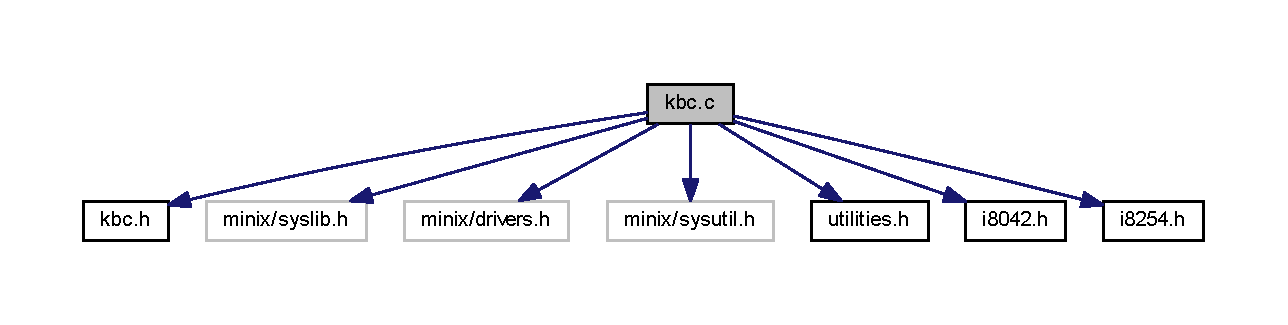
\includegraphics[width=350pt]{kbc_8c__incl}
\end{center}
\end{figure}
\subsection*{Functions}
\begin{DoxyCompactItemize}
\item 
int \hyperlink{group__kbc_ga8efa408da2468eaa11a0c515dfa8d79f}{kbd\+\_\+subscribe\+\_\+int} (unsigned int $\ast$kbd\+\_\+hook\+\_\+id)
\begin{DoxyCompactList}\small\item\em subscribes a keyboard interruption \end{DoxyCompactList}\item 
int \hyperlink{group__kbc_ga32ab97f6b806fa3a0524e62af55aeb0e}{kbd\+\_\+unsubscribe\+\_\+int} (unsigned int $\ast$kbd\+\_\+hook\+\_\+id)
\begin{DoxyCompactList}\small\item\em unsubscribes a keyboard interruption \end{DoxyCompactList}\item 
int \hyperlink{group__kbc_gad9d71d9448d7e3796e22f696863b7453}{kbc\+\_\+cmd\+\_\+read} (unsigned long $\ast$data)
\begin{DoxyCompactList}\small\item\em reads a command from kbc \end{DoxyCompactList}\item 
int \hyperlink{group__kbc_ga54b191a4ae0a5ed8d23e31cd50eb4868}{kbc\+\_\+cmd\+\_\+issue} (unsigned long cmd)
\begin{DoxyCompactList}\small\item\em issues a command to kbc \end{DoxyCompactList}\item 
int \hyperlink{group__kbc_gaa8b3453e895793f84cfc40e9cf04dd03}{kbd\+\_\+cmd\+\_\+issue} (unsigned long cmd)
\begin{DoxyCompactList}\small\item\em issues a command to kbd \end{DoxyCompactList}\item 
int \hyperlink{group__kbc_ga9a48bf91bd53208baa5627dd2a39e24d}{kbd\+\_\+cmd\+\_\+write} (unsigned int n, unsigned long $\ast$cmds)
\begin{DoxyCompactList}\small\item\em writes a complete command to kbd this function is different from the previous one because in this case it has to write several bits to kbd \end{DoxyCompactList}\item 
int \hyperlink{group__kbc_gac76f743c998918d5ff65403aa35c8b05}{kbc\+\_\+c\+\_\+to\+\_\+ass} (unsigned long $\ast$scancode)
\begin{DoxyCompactList}\small\item\em converts a variable passed buy reference to a pointer that can be interpreted in assembly \end{DoxyCompactList}\end{DoxyCompactItemize}

\hypertarget{kbc_8h}{}\section{kbc.\+h File Reference}
\label{kbc_8h}\index{kbc.\+h@{kbc.\+h}}
This graph shows which files directly or indirectly include this file\+:
\nopagebreak
\begin{figure}[H]
\begin{center}
\leavevmode
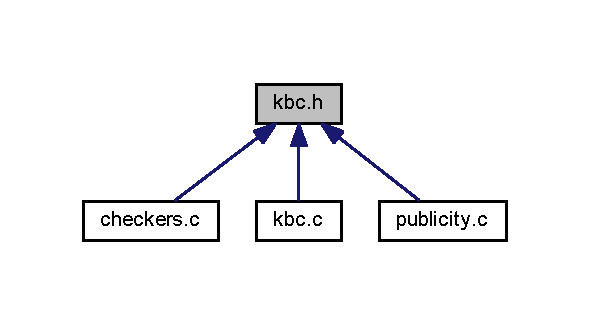
\includegraphics[width=283pt]{kbc_8h__dep__incl}
\end{center}
\end{figure}
\subsection*{Functions}
\begin{DoxyCompactItemize}
\item 
int \hyperlink{group__kbc_ga8efa408da2468eaa11a0c515dfa8d79f}{kbd\+\_\+subscribe\+\_\+int} (unsigned int $\ast$kbd\+\_\+hook\+\_\+id)
\begin{DoxyCompactList}\small\item\em subscribes a keyboard interruption \end{DoxyCompactList}\item 
int \hyperlink{group__kbc_ga32ab97f6b806fa3a0524e62af55aeb0e}{kbd\+\_\+unsubscribe\+\_\+int} (unsigned int $\ast$kbd\+\_\+hook\+\_\+id)
\begin{DoxyCompactList}\small\item\em unsubscribes a keyboard interruption \end{DoxyCompactList}\item 
int \hyperlink{group__kbc_gad9d71d9448d7e3796e22f696863b7453}{kbc\+\_\+cmd\+\_\+read} (unsigned long $\ast$data)
\begin{DoxyCompactList}\small\item\em reads a command from kbc \end{DoxyCompactList}\item 
int \hyperlink{group__kbc_ga54b191a4ae0a5ed8d23e31cd50eb4868}{kbc\+\_\+cmd\+\_\+issue} (unsigned long cmd)
\begin{DoxyCompactList}\small\item\em issues a command to kbc \end{DoxyCompactList}\item 
int \hyperlink{group__kbc_gaa8b3453e895793f84cfc40e9cf04dd03}{kbd\+\_\+cmd\+\_\+issue} (unsigned long cmd)
\begin{DoxyCompactList}\small\item\em issues a command to kbd \end{DoxyCompactList}\item 
int \hyperlink{group__kbc_ga9a48bf91bd53208baa5627dd2a39e24d}{kbd\+\_\+cmd\+\_\+write} (unsigned int n, unsigned long $\ast$cmds)
\begin{DoxyCompactList}\small\item\em writes a complete command to kbd this function is different from the previous one because in this case it has to write several bits to kbd \end{DoxyCompactList}\item 
int \hyperlink{group__kbc_gac76f743c998918d5ff65403aa35c8b05}{kbc\+\_\+c\+\_\+to\+\_\+ass} (unsigned long $\ast$scancode)
\begin{DoxyCompactList}\small\item\em converts a variable passed buy reference to a pointer that can be interpreted in assembly \end{DoxyCompactList}\end{DoxyCompactItemize}

\hypertarget{lmlib_8h}{}\section{lmlib.\+h File Reference}
\label{lmlib_8h}\index{lmlib.\+h@{lmlib.\+h}}
This graph shows which files directly or indirectly include this file\+:
\nopagebreak
\begin{figure}[H]
\begin{center}
\leavevmode
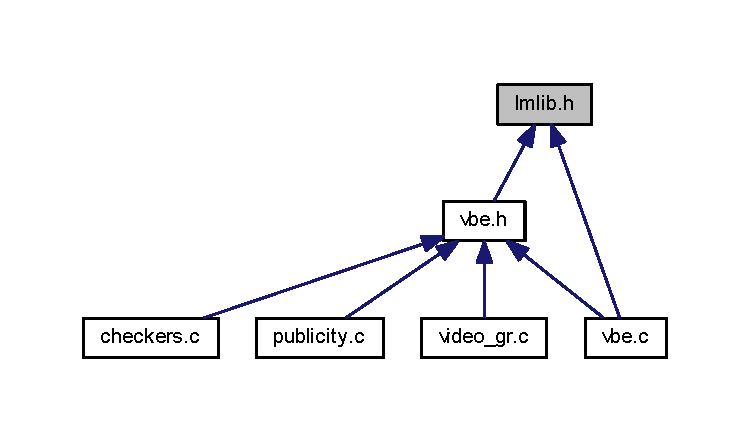
\includegraphics[width=350pt]{lmlib_8h__dep__incl}
\end{center}
\end{figure}
\subsection*{Data Structures}
\begin{DoxyCompactItemize}
\item 
struct \hyperlink{structmmap__t}{mmap\+\_\+t}
\begin{DoxyCompactList}\small\item\em Memory Map Struct. \end{DoxyCompactList}\end{DoxyCompactItemize}
\subsection*{Functions}
\begin{DoxyCompactItemize}
\item 
void $\ast$ \hyperlink{group__lmlib_ga00a9c17c01e794a6bfc80fc5c6ab1ed1}{lm\+\_\+init} (void)
\begin{DoxyCompactList}\small\item\em Initializes the low memory area, the region up to the 1 M\+Byte physical address, by mapping it on the process\textquotesingle{} physical memory address. \end{DoxyCompactList}\item 
void $\ast$ \hyperlink{group__lmlib_gae45d971ce2ffcf4dc2677eba033a92cd}{lm\+\_\+alloc} (unsigned long size, \hyperlink{structmmap__t}{mmap\+\_\+t} $\ast$map)
\begin{DoxyCompactList}\small\item\em Allocates a memory block in low memory area with the specified size. \end{DoxyCompactList}\item 
void \hyperlink{group__lmlib_ga73e89d9c297b7390021fb545513579c6}{lm\+\_\+free} (\hyperlink{structmmap__t}{mmap\+\_\+t} $\ast$map)
\begin{DoxyCompactList}\small\item\em Frees a memory block in the low memory area, previously allocated using \hyperlink{group__lmlib_gae45d971ce2ffcf4dc2677eba033a92cd}{lm\+\_\+alloc()} \end{DoxyCompactList}\end{DoxyCompactItemize}

\hypertarget{mouse_8c}{}\section{mouse.\+c File Reference}
\label{mouse_8c}\index{mouse.\+c@{mouse.\+c}}
{\ttfamily \#include \char`\"{}mouse.\+h\char`\"{}}\newline
{\ttfamily \#include $<$minix/syslib.\+h$>$}\newline
{\ttfamily \#include $<$minix/drivers.\+h$>$}\newline
{\ttfamily \#include $<$minix/sysutil.\+h$>$}\newline
{\ttfamily \#include \char`\"{}video\+\_\+gr.\+h\char`\"{}}\newline
{\ttfamily \#include \char`\"{}utilities.\+h\char`\"{}}\newline
{\ttfamily \#include \char`\"{}i8042.\+h\char`\"{}}\newline
{\ttfamily \#include \char`\"{}i8254.\+h\char`\"{}}\newline
Include dependency graph for mouse.\+c\+:
\nopagebreak
\begin{figure}[H]
\begin{center}
\leavevmode
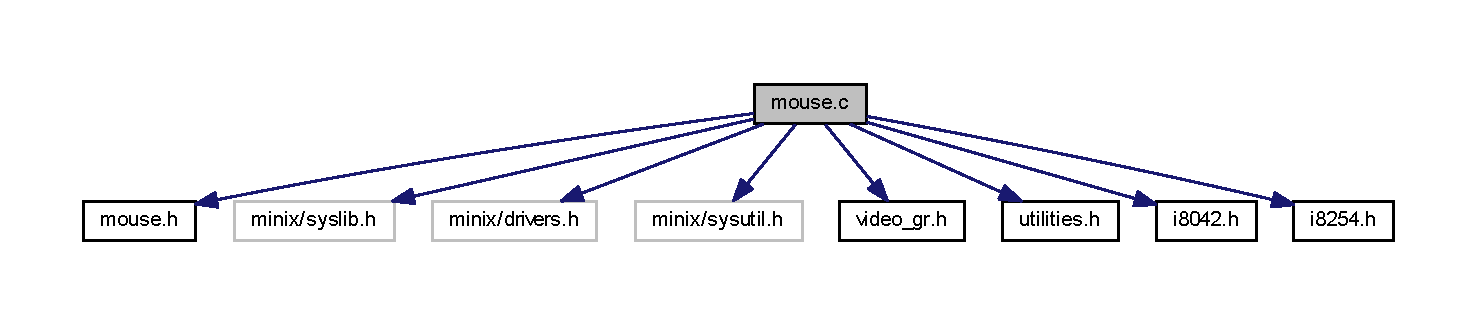
\includegraphics[width=350pt]{mouse_8c__incl}
\end{center}
\end{figure}
\subsection*{Functions}
\begin{DoxyCompactItemize}
\item 
int \hyperlink{group__mouse_gad607aaa8fd9833789fcd2b99c86dfc34}{mouse\+\_\+subscribe\+\_\+int} (unsigned int $\ast$mouse\+\_\+hook\+\_\+id)
\begin{DoxyCompactList}\small\item\em subscribes a mouse interruption \end{DoxyCompactList}\item 
int \hyperlink{group__mouse_gaa40354aab63adaf9ecddd01255efd918}{mouse\+\_\+unsubscribe\+\_\+int} (unsigned int $\ast$mouse\+\_\+hook\+\_\+id)
\begin{DoxyCompactList}\small\item\em unsubscribes a timer interruption \end{DoxyCompactList}\item 
int \hyperlink{group__mouse_ga42d943d35caacd5219cf4ef665b9bc42}{mouse\+\_\+cmd\+\_\+write} (unsigned long cmd)
\begin{DoxyCompactList}\small\item\em writes a command to kbd \end{DoxyCompactList}\item 
int \hyperlink{group__mouse_ga3a8a668ee784e6662fb1c2fd31e811b0}{mouse\+\_\+cmd\+\_\+read} (unsigned long $\ast$data)
\begin{DoxyCompactList}\small\item\em reads a command from mouse \end{DoxyCompactList}\item 
int \hyperlink{group__mouse_ga936c78f40a1d0b1acfd4f0368a9b8137}{mouse\+\_\+get\+\_\+packet} (unsigned long $\ast$next\+\_\+byte, unsigned char $\ast$packet)
\begin{DoxyCompactList}\small\item\em gets a packet from mouse \end{DoxyCompactList}\item 
void \hyperlink{group__mouse_gaf1a4587fac965330aca5079ae1313327}{mouse\+\_\+convert\+\_\+packet} (unsigned char $\ast$array\+\_\+packet, \hyperlink{structmouse__packet__t}{mouse\+\_\+packet\+\_\+t} $\ast$packet)
\begin{DoxyCompactList}\small\item\em convert a packet array to mouse packet that is more user friendly \end{DoxyCompactList}\end{DoxyCompactItemize}

\hypertarget{mouse_8h}{}\section{mouse.\+h File Reference}
\label{mouse_8h}\index{mouse.\+h@{mouse.\+h}}
This graph shows which files directly or indirectly include this file\+:
\nopagebreak
\begin{figure}[H]
\begin{center}
\leavevmode
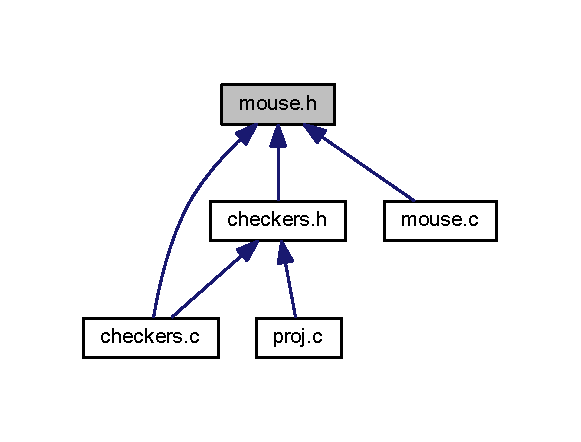
\includegraphics[width=279pt]{mouse_8h__dep__incl}
\end{center}
\end{figure}
\subsection*{Data Structures}
\begin{DoxyCompactItemize}
\item 
struct \hyperlink{structmouse__packet__t}{mouse\+\_\+packet\+\_\+t}
\end{DoxyCompactItemize}
\subsection*{Functions}
\begin{DoxyCompactItemize}
\item 
int \hyperlink{group__mouse_gad607aaa8fd9833789fcd2b99c86dfc34}{mouse\+\_\+subscribe\+\_\+int} (unsigned int $\ast$mouse\+\_\+hook\+\_\+id)
\begin{DoxyCompactList}\small\item\em subscribes a mouse interruption \end{DoxyCompactList}\item 
int \hyperlink{group__mouse_gaa40354aab63adaf9ecddd01255efd918}{mouse\+\_\+unsubscribe\+\_\+int} (unsigned int $\ast$mouse\+\_\+hook\+\_\+id)
\begin{DoxyCompactList}\small\item\em unsubscribes a timer interruption \end{DoxyCompactList}\item 
int \hyperlink{group__mouse_ga42d943d35caacd5219cf4ef665b9bc42}{mouse\+\_\+cmd\+\_\+write} (unsigned long cmd)
\begin{DoxyCompactList}\small\item\em writes a command to kbd \end{DoxyCompactList}\item 
int \hyperlink{group__mouse_ga3a8a668ee784e6662fb1c2fd31e811b0}{mouse\+\_\+cmd\+\_\+read} (unsigned long $\ast$data)
\begin{DoxyCompactList}\small\item\em reads a command from mouse \end{DoxyCompactList}\item 
int \hyperlink{group__mouse_ga936c78f40a1d0b1acfd4f0368a9b8137}{mouse\+\_\+get\+\_\+packet} (unsigned long $\ast$next\+\_\+byte, unsigned char $\ast$packet)
\begin{DoxyCompactList}\small\item\em gets a packet from mouse \end{DoxyCompactList}\item 
void \hyperlink{group__mouse_gaf1a4587fac965330aca5079ae1313327}{mouse\+\_\+convert\+\_\+packet} (unsigned char $\ast$array\+\_\+packet, \hyperlink{structmouse__packet__t}{mouse\+\_\+packet\+\_\+t} $\ast$packet)
\begin{DoxyCompactList}\small\item\em convert a packet array to mouse packet that is more user friendly \end{DoxyCompactList}\end{DoxyCompactItemize}

\hypertarget{_program_logic_8c}{}\section{Program\+Logic.\+c File Reference}
\label{_program_logic_8c}\index{Program\+Logic.\+c@{Program\+Logic.\+c}}
{\ttfamily \#include \char`\"{}Program\+Logic.\+h\char`\"{}}\newline
{\ttfamily \#include $<$stdio.\+h$>$}\newline
Include dependency graph for Program\+Logic.\+c\+:
\nopagebreak
\begin{figure}[H]
\begin{center}
\leavevmode
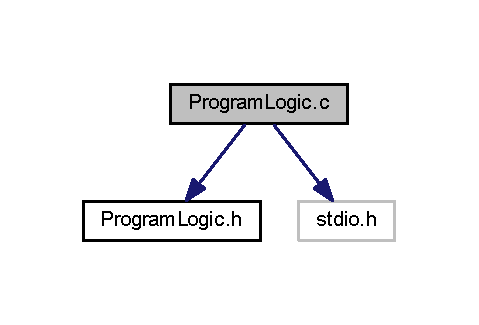
\includegraphics[width=230pt]{_program_logic_8c__incl}
\end{center}
\end{figure}
\subsection*{Functions}
\begin{DoxyCompactItemize}
\item 
int \hyperlink{group___program_logic_ga2838b9e6247aa4515f76cfeccf8e1cd8}{create\+Board} (char \hyperlink{checkers_8c_a12f50bd537a3a737da9d47710c308ae3}{board}\mbox{[}8\mbox{]}\mbox{[}8\mbox{]})
\begin{DoxyCompactList}\small\item\em Creates the board with initial positions. \end{DoxyCompactList}\item 
int \hyperlink{group___program_logic_gaed1b217c7e40a6fb27a0e6a719594aba}{is\+Position\+Initial\+Valid} (char \hyperlink{checkers_8c_a12f50bd537a3a737da9d47710c308ae3}{board}\mbox{[}8\mbox{]}\mbox{[}8\mbox{]}, char player, int xi, int yi)
\begin{DoxyCompactList}\small\item\em Verifies if given initial position(xi,yi) is valid or not. \end{DoxyCompactList}\item 
int \hyperlink{group___program_logic_ga02801d684d1f985fcaff098e12a0bf59}{move\+Disc} (char \hyperlink{checkers_8c_a12f50bd537a3a737da9d47710c308ae3}{board}\mbox{[}8\mbox{]}\mbox{[}8\mbox{]}, char player, int xi, int yi, int xf, int yf)
\begin{DoxyCompactList}\small\item\em Moves disc in the given position(xi,yi) to final position also given(xf,yf). \end{DoxyCompactList}\item 
int \hyperlink{group___program_logic_gacfd2089a907444dab0ccd2d95f321b8b}{is\+End\+Game} (char \hyperlink{checkers_8c_a12f50bd537a3a737da9d47710c308ae3}{board}\mbox{[}8\mbox{]}\mbox{[}8\mbox{]})
\begin{DoxyCompactList}\small\item\em Verifies if it is the end of the game. \end{DoxyCompactList}\item 
void \hyperlink{group___program_logic_ga484dd8982591f724c6ff6749bba6869a}{move\+To\+Final} (char \hyperlink{checkers_8c_a12f50bd537a3a737da9d47710c308ae3}{board}\mbox{[}8\mbox{]}\mbox{[}8\mbox{]}, int xi, int yi, int xf, int yf)
\begin{DoxyCompactList}\small\item\em Moves disc in the given position(xi,yi) to final position also given(xf,yf). \end{DoxyCompactList}\item 
void \hyperlink{group___program_logic_ga5de7cebab5418f009cebb5dc73e50cd2}{make\+Capture\+Move} (char \hyperlink{checkers_8c_a12f50bd537a3a737da9d47710c308ae3}{board}\mbox{[}8\mbox{]}\mbox{[}8\mbox{]}, int xi, int yi, int xf, int yf)
\begin{DoxyCompactList}\small\item\em Moves disc in the given position(xi,yi) to final position also given(xf,yf), making a capture move. \end{DoxyCompactList}\item 
int \hyperlink{group___program_logic_ga0862e9966f69666bb39dbf1c58863c3b}{verify\+Capture\+Move} (char \hyperlink{checkers_8c_a12f50bd537a3a737da9d47710c308ae3}{board}\mbox{[}8\mbox{]}\mbox{[}8\mbox{]}, char player, int xi, int yi)
\begin{DoxyCompactList}\small\item\em Verifies if given initial position(xi,yi) can do a capture move or not. \end{DoxyCompactList}\item 
int $\ast$ \hyperlink{group___program_logic_ga8d87858478876b33304e38cea751951b}{moves\+I\+Can\+Do} (char \hyperlink{checkers_8c_a12f50bd537a3a737da9d47710c308ae3}{board}\mbox{[}8\mbox{]}\mbox{[}8\mbox{]}, char player, int xi, int yi)
\begin{DoxyCompactList}\small\item\em Gives the moves that a disc can make. \end{DoxyCompactList}\end{DoxyCompactItemize}

\hypertarget{_program_logic_8h}{}\section{Program\+Logic.\+h File Reference}
\label{_program_logic_8h}\index{Program\+Logic.\+h@{Program\+Logic.\+h}}
This graph shows which files directly or indirectly include this file\+:
\nopagebreak
\begin{figure}[H]
\begin{center}
\leavevmode
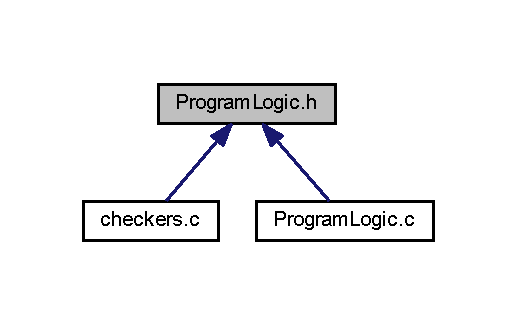
\includegraphics[width=248pt]{_program_logic_8h__dep__incl}
\end{center}
\end{figure}
\subsection*{Functions}
\begin{DoxyCompactItemize}
\item 
int \hyperlink{group___program_logic_ga2838b9e6247aa4515f76cfeccf8e1cd8}{create\+Board} (char \hyperlink{checkers_8c_a12f50bd537a3a737da9d47710c308ae3}{board}\mbox{[}8\mbox{]}\mbox{[}8\mbox{]})
\begin{DoxyCompactList}\small\item\em Creates the board with initial positions. \end{DoxyCompactList}\item 
int \hyperlink{group___program_logic_ga02801d684d1f985fcaff098e12a0bf59}{move\+Disc} (char \hyperlink{checkers_8c_a12f50bd537a3a737da9d47710c308ae3}{board}\mbox{[}8\mbox{]}\mbox{[}8\mbox{]}, char player, int xi, int yi, int xf, int yf)
\begin{DoxyCompactList}\small\item\em Moves disc in the given position(xi,yi) to final position also given(xf,yf). \end{DoxyCompactList}\item 
int \hyperlink{group___program_logic_gaed1b217c7e40a6fb27a0e6a719594aba}{is\+Position\+Initial\+Valid} (char \hyperlink{checkers_8c_a12f50bd537a3a737da9d47710c308ae3}{board}\mbox{[}8\mbox{]}\mbox{[}8\mbox{]}, char player, int xi, int yi)
\begin{DoxyCompactList}\small\item\em Verifies if given initial position(xi,yi) is valid or not. \end{DoxyCompactList}\item 
int \hyperlink{group___program_logic_ga0862e9966f69666bb39dbf1c58863c3b}{verify\+Capture\+Move} (char \hyperlink{checkers_8c_a12f50bd537a3a737da9d47710c308ae3}{board}\mbox{[}8\mbox{]}\mbox{[}8\mbox{]}, char player, int xi, int yi)
\begin{DoxyCompactList}\small\item\em Verifies if given initial position(xi,yi) can do a capture move or not. \end{DoxyCompactList}\item 
void \hyperlink{group___program_logic_ga484dd8982591f724c6ff6749bba6869a}{move\+To\+Final} (char \hyperlink{checkers_8c_a12f50bd537a3a737da9d47710c308ae3}{board}\mbox{[}8\mbox{]}\mbox{[}8\mbox{]}, int xi, int yi, int xf, int yf)
\begin{DoxyCompactList}\small\item\em Moves disc in the given position(xi,yi) to final position also given(xf,yf). \end{DoxyCompactList}\item 
void \hyperlink{group___program_logic_ga5de7cebab5418f009cebb5dc73e50cd2}{make\+Capture\+Move} (char \hyperlink{checkers_8c_a12f50bd537a3a737da9d47710c308ae3}{board}\mbox{[}8\mbox{]}\mbox{[}8\mbox{]}, int xi, int yi, int xf, int yf)
\begin{DoxyCompactList}\small\item\em Moves disc in the given position(xi,yi) to final position also given(xf,yf), making a capture move. \end{DoxyCompactList}\item 
int \hyperlink{group___program_logic_gacfd2089a907444dab0ccd2d95f321b8b}{is\+End\+Game} (char \hyperlink{checkers_8c_a12f50bd537a3a737da9d47710c308ae3}{board}\mbox{[}8\mbox{]}\mbox{[}8\mbox{]})
\begin{DoxyCompactList}\small\item\em Verifies if it is the end of the game. \end{DoxyCompactList}\item 
int $\ast$ \hyperlink{group___program_logic_ga8d87858478876b33304e38cea751951b}{moves\+I\+Can\+Do} (char \hyperlink{checkers_8c_a12f50bd537a3a737da9d47710c308ae3}{board}\mbox{[}8\mbox{]}\mbox{[}8\mbox{]}, char player, int xi, int yi)
\begin{DoxyCompactList}\small\item\em Gives the moves that a disc can make. \end{DoxyCompactList}\end{DoxyCompactItemize}

\hypertarget{proj_8c}{}\section{proj.\+c File Reference}
\label{proj_8c}\index{proj.\+c@{proj.\+c}}
{\ttfamily \#include $<$limits.\+h$>$}\newline
{\ttfamily \#include $<$string.\+h$>$}\newline
{\ttfamily \#include $<$errno.\+h$>$}\newline
{\ttfamily \#include $<$minix/drivers.\+h$>$}\newline
{\ttfamily \#include \char`\"{}checkers.\+h\char`\"{}}\newline
{\ttfamily \#include \char`\"{}utilities.\+h\char`\"{}}\newline
{\ttfamily \#include \char`\"{}proj.\+h\char`\"{}}\newline
{\ttfamily \#include \char`\"{}ser\+\_\+port.\+h\char`\"{}}\newline
Include dependency graph for proj.\+c\+:
\nopagebreak
\begin{figure}[H]
\begin{center}
\leavevmode
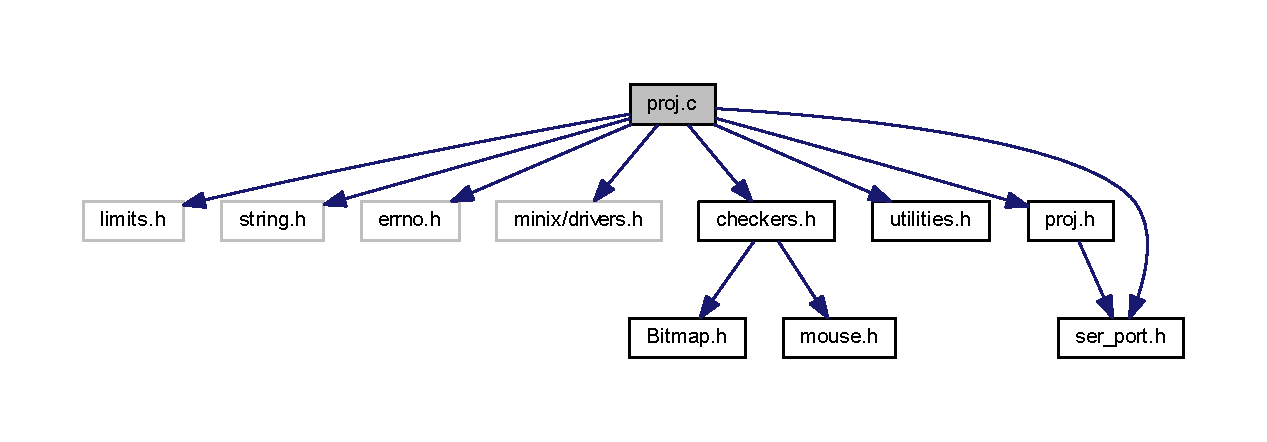
\includegraphics[width=350pt]{proj_8c__incl}
\end{center}
\end{figure}
\subsection*{Functions}
\begin{DoxyCompactItemize}
\item 
static void \hyperlink{proj_8c_a7721a8566abc323f59672fdde30d3e20}{print\+\_\+usage} (char $\ast$$\ast$argv)
\item 
static int \hyperlink{proj_8c_a97b25d50dc55b5c8c2315fd010bc2957}{proc\+\_\+args} (int argc, char $\ast$$\ast$argv)
\item 
static void \hyperlink{proj_8c_a3310cf47c29dd0f685c58e04fac7be4a}{ret\+\_\+path\+\_\+images} (char $\ast$arg, char $\ast$path\+\_\+images)
\item 
int \hyperlink{group__proj_ga3c04138a5bfe5d72780bb7e82a18e627}{main} (int argc, char $\ast$$\ast$argv)
\begin{DoxyCompactList}\small\item\em Main Function. \end{DoxyCompactList}\item 
int \hyperlink{group__proj_gac4a55a52afabd10db600de603282ff99}{connect\+\_\+serial} (char player, char $\ast$arg0)
\begin{DoxyCompactList}\small\item\em establishes a connection in the serial port \end{DoxyCompactList}\end{DoxyCompactItemize}


\subsection{Function Documentation}
\hypertarget{proj_8c_a7721a8566abc323f59672fdde30d3e20}{}\label{proj_8c_a7721a8566abc323f59672fdde30d3e20} 
\index{proj.\+c@{proj.\+c}!print\+\_\+usage@{print\+\_\+usage}}
\index{print\+\_\+usage@{print\+\_\+usage}!proj.\+c@{proj.\+c}}
\subsubsection{\texorpdfstring{print\+\_\+usage()}{print\_usage()}}
{\footnotesize\ttfamily static void print\+\_\+usage (\begin{DoxyParamCaption}\item[{char $\ast$$\ast$}]{argv }\end{DoxyParamCaption})\hspace{0.3cm}{\ttfamily [static]}}

\hypertarget{proj_8c_a97b25d50dc55b5c8c2315fd010bc2957}{}\label{proj_8c_a97b25d50dc55b5c8c2315fd010bc2957} 
\index{proj.\+c@{proj.\+c}!proc\+\_\+args@{proc\+\_\+args}}
\index{proc\+\_\+args@{proc\+\_\+args}!proj.\+c@{proj.\+c}}
\subsubsection{\texorpdfstring{proc\+\_\+args()}{proc\_args()}}
{\footnotesize\ttfamily static int proc\+\_\+args (\begin{DoxyParamCaption}\item[{int}]{argc,  }\item[{char $\ast$$\ast$}]{argv }\end{DoxyParamCaption})\hspace{0.3cm}{\ttfamily [static]}}

Here is the call graph for this function\+:
\nopagebreak
\begin{figure}[H]
\begin{center}
\leavevmode
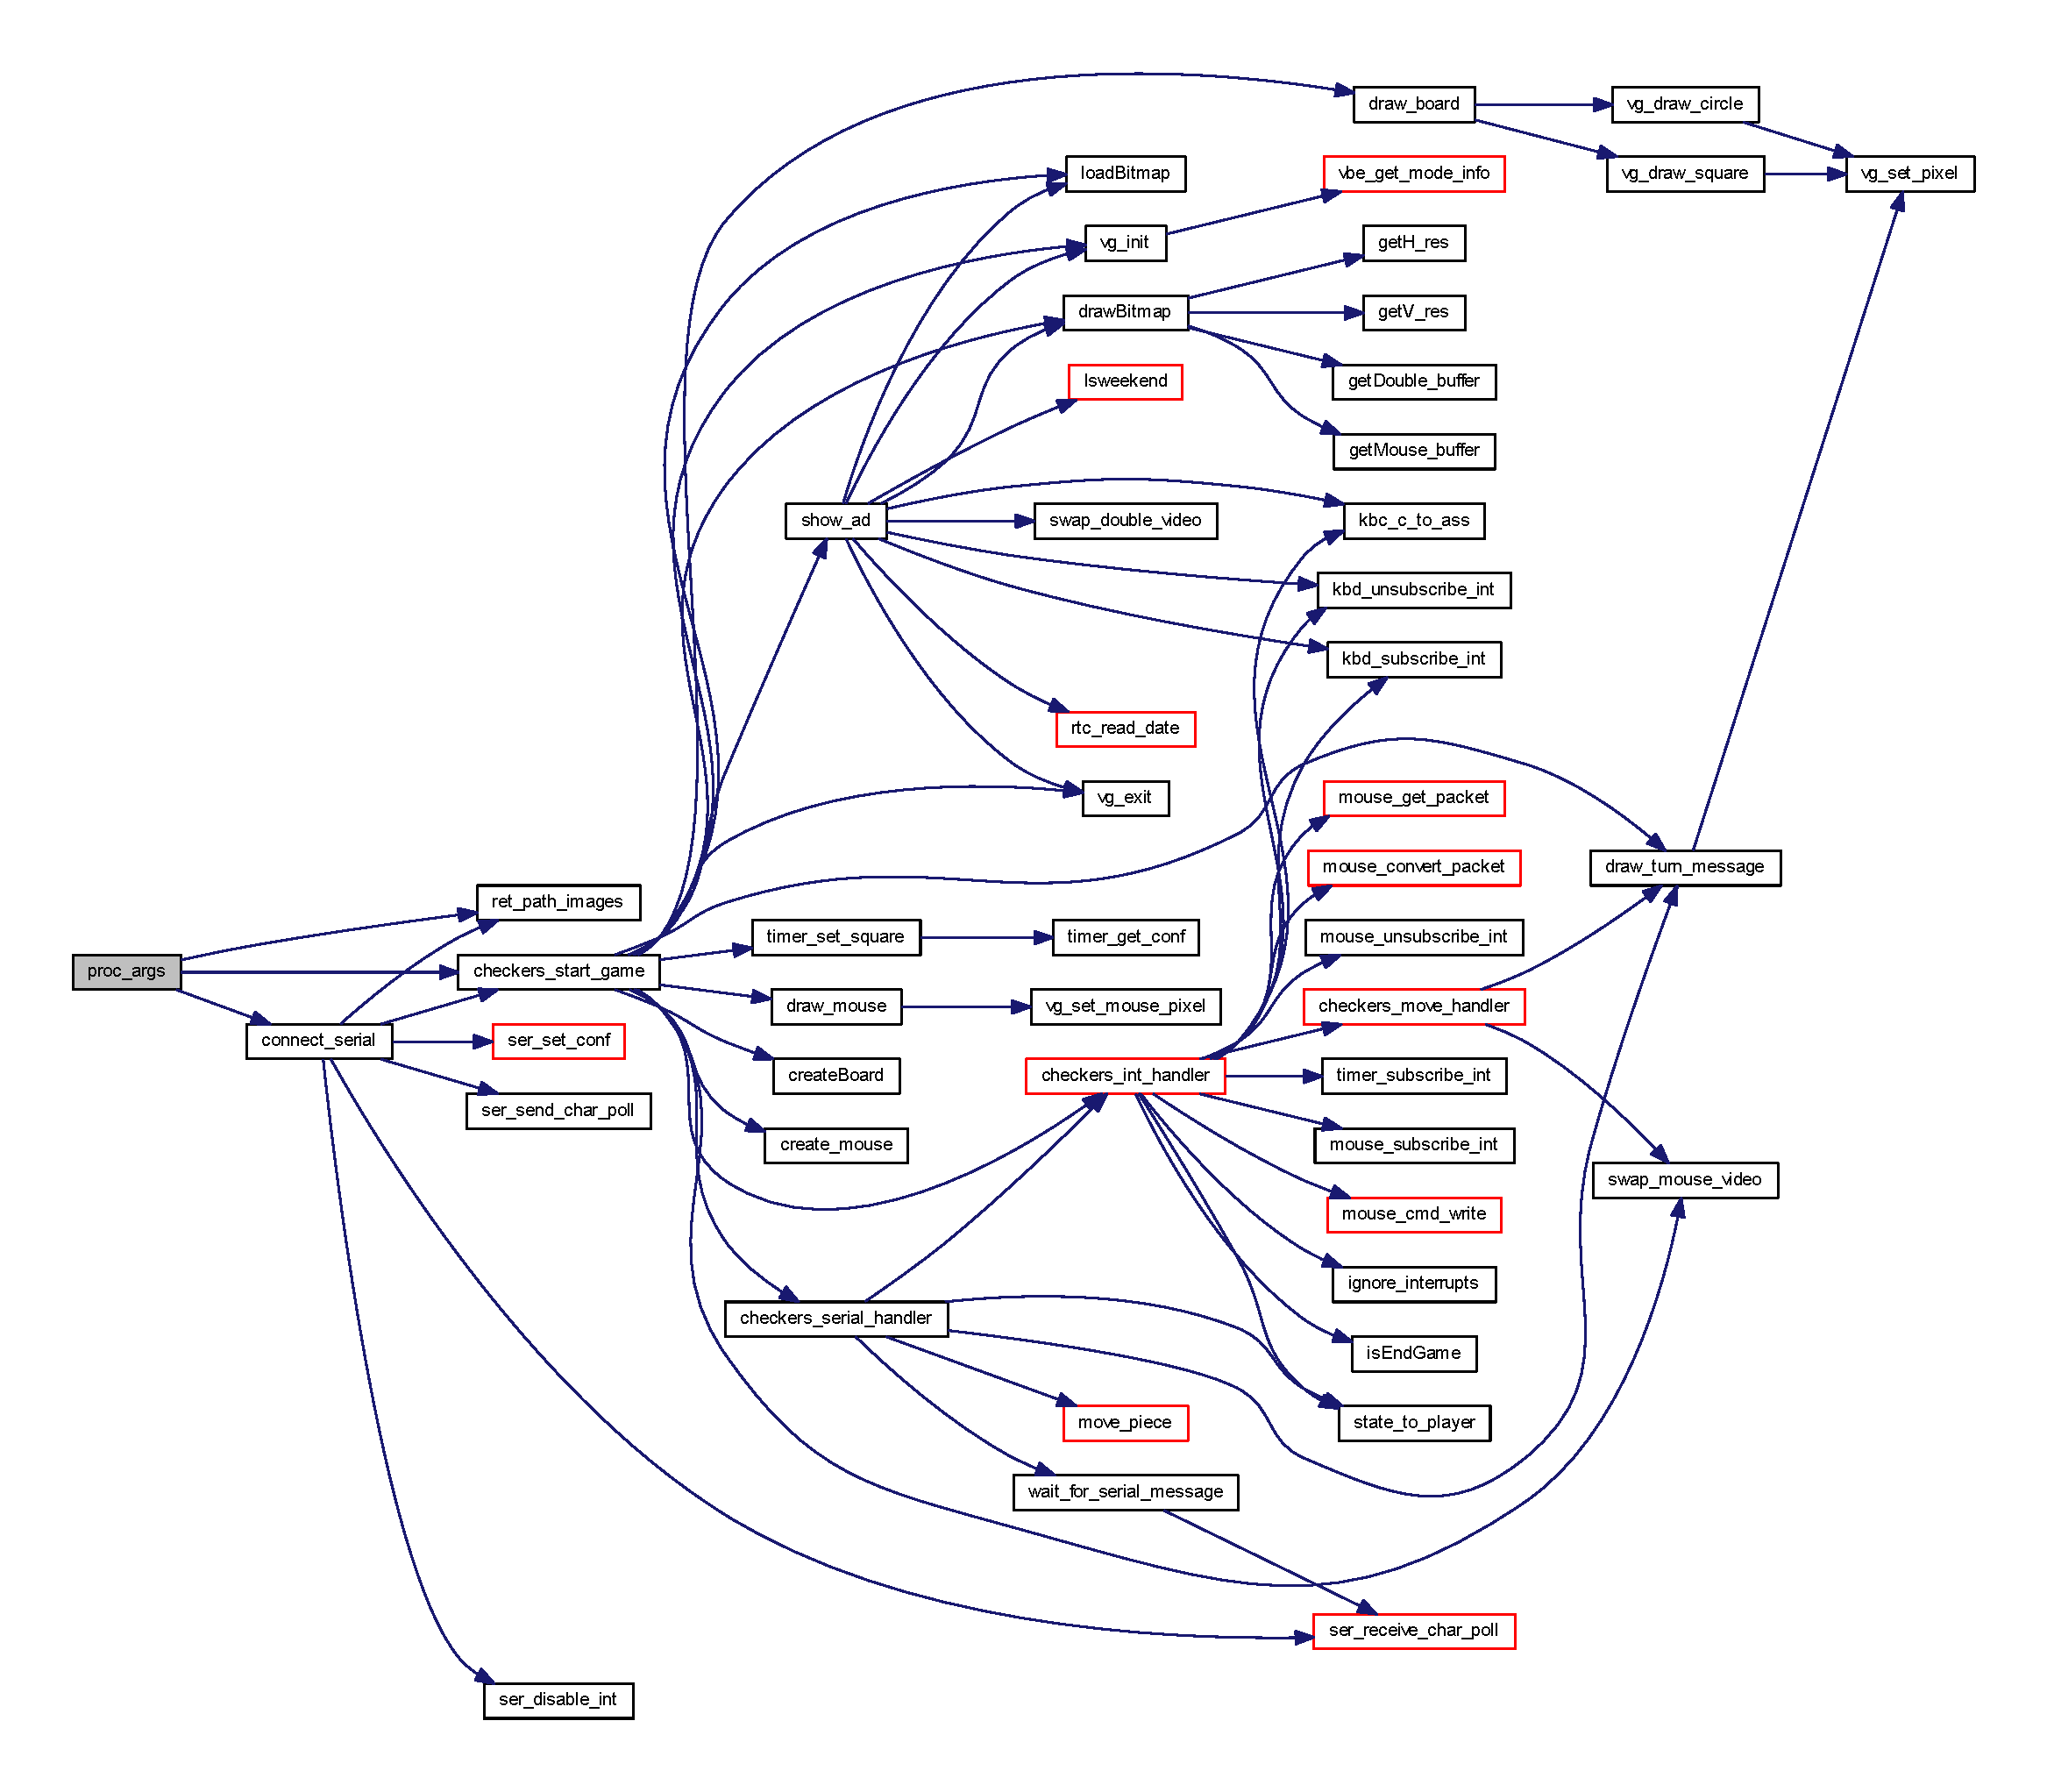
\includegraphics[width=350pt]{proj_8c_a97b25d50dc55b5c8c2315fd010bc2957_cgraph}
\end{center}
\end{figure}
\hypertarget{proj_8c_a3310cf47c29dd0f685c58e04fac7be4a}{}\label{proj_8c_a3310cf47c29dd0f685c58e04fac7be4a} 
\index{proj.\+c@{proj.\+c}!ret\+\_\+path\+\_\+images@{ret\+\_\+path\+\_\+images}}
\index{ret\+\_\+path\+\_\+images@{ret\+\_\+path\+\_\+images}!proj.\+c@{proj.\+c}}
\subsubsection{\texorpdfstring{ret\+\_\+path\+\_\+images()}{ret\_path\_images()}}
{\footnotesize\ttfamily static void ret\+\_\+path\+\_\+images (\begin{DoxyParamCaption}\item[{char $\ast$}]{arg,  }\item[{char $\ast$}]{path\+\_\+images }\end{DoxyParamCaption})\hspace{0.3cm}{\ttfamily [static]}}


\hypertarget{proj_8h}{}\section{proj.\+h File Reference}
\label{proj_8h}\index{proj.\+h@{proj.\+h}}
{\ttfamily \#include \char`\"{}ser\+\_\+port.\+h\char`\"{}}\newline
Include dependency graph for proj.\+h\+:
\nopagebreak
\begin{figure}[H]
\begin{center}
\leavevmode
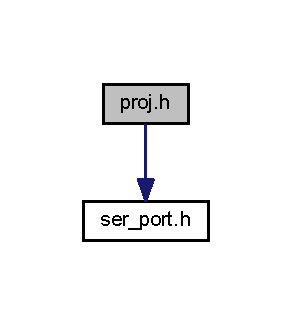
\includegraphics[width=140pt]{proj_8h__incl}
\end{center}
\end{figure}
This graph shows which files directly or indirectly include this file\+:
\nopagebreak
\begin{figure}[H]
\begin{center}
\leavevmode
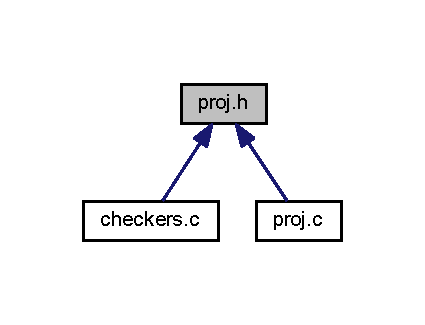
\includegraphics[width=204pt]{proj_8h__dep__incl}
\end{center}
\end{figure}
\subsection*{Macros}
\begin{DoxyCompactItemize}
\item 
\#define \hyperlink{group__proj_ga698fc99ce97e8051ede3e8e9c9baaaf1}{P\+O\+R\+T\+\_\+\+A\+D\+DR}~\hyperlink{group__ser__port_ga98199cd85fbe47b9a741b07762260422}{S\+E\+R\+\_\+\+C\+O\+M1\+\_\+\+A\+D\+DR}
\item 
\#define \hyperlink{group__proj_ga108355009766d90bac37c294fad39ca5}{P\+O\+R\+T\+\_\+\+B\+I\+TS}~8
\item 
\#define \hyperlink{group__proj_ga31b06d45be51d1c232d4cb34be4d385b}{P\+O\+R\+T\+\_\+\+S\+T\+OP}~2
\item 
\#define \hyperlink{group__proj_gaf868e5bf4fd27a5f53de530ce879dee4}{P\+O\+R\+T\+\_\+\+P\+A\+R\+I\+TY}~0
\item 
\#define \hyperlink{group__proj_gaa892a49ac9cab99bd99907f48a535b72}{P\+O\+R\+T\+\_\+\+R\+A\+TE}~9600
\end{DoxyCompactItemize}
\subsection*{Functions}
\begin{DoxyCompactItemize}
\item 
int \hyperlink{group__proj_ga3c04138a5bfe5d72780bb7e82a18e627}{main} (int argc, char $\ast$$\ast$argv)
\begin{DoxyCompactList}\small\item\em Main Function. \end{DoxyCompactList}\item 
static void \hyperlink{group__proj_ga7721a8566abc323f59672fdde30d3e20}{print\+\_\+usage} (char $\ast$$\ast$argv)
\begin{DoxyCompactList}\small\item\em print\+\_\+usage \end{DoxyCompactList}\item 
static int \hyperlink{group__proj_ga97b25d50dc55b5c8c2315fd010bc2957}{proc\+\_\+args} (int argc, char $\ast$$\ast$argv)
\begin{DoxyCompactList}\small\item\em print\+\_\+args \end{DoxyCompactList}\item 
static void \hyperlink{group__proj_ga3310cf47c29dd0f685c58e04fac7be4a}{ret\+\_\+path\+\_\+images} (char $\ast$arg, char $\ast$path\+\_\+images)
\begin{DoxyCompactList}\small\item\em ret\+\_\+path\+\_\+images \end{DoxyCompactList}\item 
int \hyperlink{group__proj_gac4a55a52afabd10db600de603282ff99}{connect\+\_\+serial} (char player, char $\ast$arg0)
\begin{DoxyCompactList}\small\item\em establishes a connection in the serial port \end{DoxyCompactList}\end{DoxyCompactItemize}

\hypertarget{publicity_8c}{}\section{publicity.\+c File Reference}
\label{publicity_8c}\index{publicity.\+c@{publicity.\+c}}
{\ttfamily \#include $<$errno.\+h$>$}\newline
{\ttfamily \#include $<$minix/drivers.\+h$>$}\newline
{\ttfamily \#include $<$limits.\+h$>$}\newline
{\ttfamily \#include $<$string.\+h$>$}\newline
{\ttfamily \#include $<$stdlib.\+h$>$}\newline
{\ttfamily \#include $<$stdarg.\+h$>$}\newline
{\ttfamily \#include \char`\"{}Bitmap.\+h\char`\"{}}\newline
{\ttfamily \#include \char`\"{}utilities.\+h\char`\"{}}\newline
{\ttfamily \#include \char`\"{}rtc.\+h\char`\"{}}\newline
{\ttfamily \#include \char`\"{}video\+\_\+gr.\+h\char`\"{}}\newline
{\ttfamily \#include \char`\"{}vbe.\+h\char`\"{}}\newline
{\ttfamily \#include \char`\"{}kbc.\+h\char`\"{}}\newline
{\ttfamily \#include \char`\"{}i8042.\+h\char`\"{}}\newline
Include dependency graph for publicity.\+c\+:
\nopagebreak
\begin{figure}[H]
\begin{center}
\leavevmode
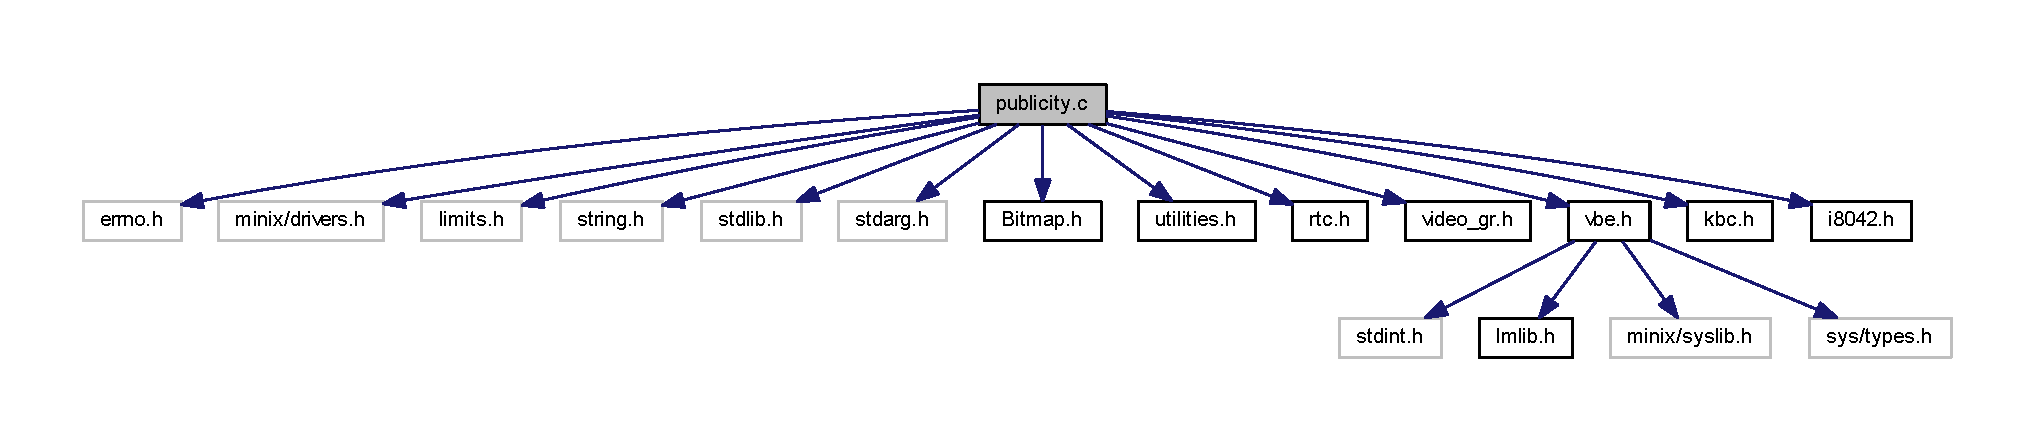
\includegraphics[width=350pt]{publicity_8c__incl}
\end{center}
\end{figure}
\subsection*{Functions}
\begin{DoxyCompactItemize}
\item 
int \hyperlink{group__publicity_ga7a04ef3aec214c81663352a9f4f35a65}{show\+\_\+ad} (char $\ast$path\+\_\+images)
\begin{DoxyCompactList}\small\item\em shows an ad. If today is a day of the week shows a certain ad, if it\textquotesingle{}s weekend shows another one \end{DoxyCompactList}\item 
int \hyperlink{group__publicity_ga7bad5577543cdab533e3bc88669cd691}{Isweekend} (\hyperlink{structdate__t}{date\+\_\+t} date)
\begin{DoxyCompactList}\small\item\em Determines if date is a weekend or not. \end{DoxyCompactList}\item 
int \hyperlink{group__publicity_ga2ff0d1265d48a43111f38f357dd1f874}{Isleap} (int year)
\begin{DoxyCompactList}\small\item\em Determines is year is leap or not. \end{DoxyCompactList}\end{DoxyCompactItemize}
\subsection*{Variables}
\begin{DoxyCompactItemize}
\item 
static \hyperlink{struct_bitmap}{Bitmap} $\ast$ \hyperlink{publicity_8c_a4bdaa00739a5ab865fc068c7fecd84b0}{ad\+\_\+week}
\item 
static \hyperlink{struct_bitmap}{Bitmap} $\ast$ \hyperlink{publicity_8c_add3382a8eebd682a2b6add2d78f07010}{ad\+\_\+weekend}
\end{DoxyCompactItemize}


\subsection{Variable Documentation}
\hypertarget{publicity_8c_a4bdaa00739a5ab865fc068c7fecd84b0}{}\label{publicity_8c_a4bdaa00739a5ab865fc068c7fecd84b0} 
\index{publicity.\+c@{publicity.\+c}!ad\+\_\+week@{ad\+\_\+week}}
\index{ad\+\_\+week@{ad\+\_\+week}!publicity.\+c@{publicity.\+c}}
\subsubsection{\texorpdfstring{ad\+\_\+week}{ad\_week}}
{\footnotesize\ttfamily \hyperlink{struct_bitmap}{Bitmap}$\ast$ ad\+\_\+week\hspace{0.3cm}{\ttfamily [static]}}

\hypertarget{publicity_8c_add3382a8eebd682a2b6add2d78f07010}{}\label{publicity_8c_add3382a8eebd682a2b6add2d78f07010} 
\index{publicity.\+c@{publicity.\+c}!ad\+\_\+weekend@{ad\+\_\+weekend}}
\index{ad\+\_\+weekend@{ad\+\_\+weekend}!publicity.\+c@{publicity.\+c}}
\subsubsection{\texorpdfstring{ad\+\_\+weekend}{ad\_weekend}}
{\footnotesize\ttfamily \hyperlink{struct_bitmap}{Bitmap}$\ast$ ad\+\_\+weekend\hspace{0.3cm}{\ttfamily [static]}}


\hypertarget{publicity_8h}{}\section{publicity.\+h File Reference}
\label{publicity_8h}\index{publicity.\+h@{publicity.\+h}}
This graph shows which files directly or indirectly include this file\+:
\nopagebreak
\begin{figure}[H]
\begin{center}
\leavevmode
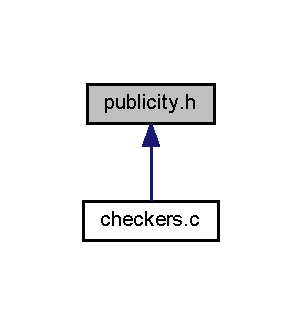
\includegraphics[width=145pt]{publicity_8h__dep__incl}
\end{center}
\end{figure}
\subsection*{Functions}
\begin{DoxyCompactItemize}
\item 
int \hyperlink{group__publicity_ga7a04ef3aec214c81663352a9f4f35a65}{show\+\_\+ad} (char $\ast$path\+\_\+images)
\begin{DoxyCompactList}\small\item\em shows an ad. If today is a day of the week shows a certain ad, if it\textquotesingle{}s weekend shows another one \end{DoxyCompactList}\item 
int \hyperlink{group__publicity_ga7bad5577543cdab533e3bc88669cd691}{Isweekend} (\hyperlink{structdate__t}{date\+\_\+t} date)
\begin{DoxyCompactList}\small\item\em Determines if date is a weekend or not. \end{DoxyCompactList}\item 
int \hyperlink{group__publicity_ga2ff0d1265d48a43111f38f357dd1f874}{Isleap} (int year)
\begin{DoxyCompactList}\small\item\em Determines is year is leap or not. \end{DoxyCompactList}\end{DoxyCompactItemize}

\hypertarget{rtc_8c}{}\section{rtc.\+c File Reference}
\label{rtc_8c}\index{rtc.\+c@{rtc.\+c}}
{\ttfamily \#include $<$minix/syslib.\+h$>$}\newline
{\ttfamily \#include $<$minix/drivers.\+h$>$}\newline
{\ttfamily \#include $<$minix/sysutil.\+h$>$}\newline
{\ttfamily \#include \char`\"{}rtc.\+h\char`\"{}}\newline
{\ttfamily \#include \char`\"{}utilities.\+h\char`\"{}}\newline
Include dependency graph for rtc.\+c\+:
\nopagebreak
\begin{figure}[H]
\begin{center}
\leavevmode
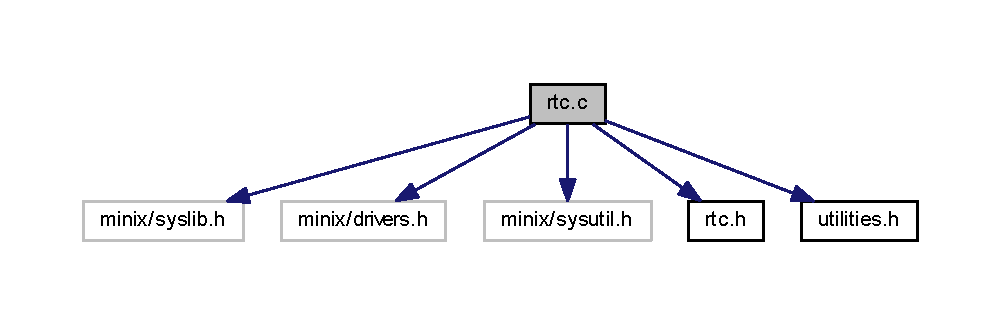
\includegraphics[width=350pt]{rtc_8c__incl}
\end{center}
\end{figure}
\subsection*{Macros}
\begin{DoxyCompactItemize}
\item 
\#define \hyperlink{rtc_8c_a3a8ea58898cb58fc96013383d39f482c}{B\+IT}(n)~(0x01$<$$<$(n))
\end{DoxyCompactItemize}
\subsection*{Functions}
\begin{DoxyCompactItemize}
\item 
int \hyperlink{group__rtc_ga3b9f4583bad77c33ea0e82c1c1ad5305}{rtc\+\_\+subscribe\+\_\+int} (unsigned int $\ast$rtc\+\_\+hook\+\_\+id)
\begin{DoxyCompactList}\small\item\em subscribes a R\+TC interruption \end{DoxyCompactList}\item 
int \hyperlink{group__rtc_ga61932ec1f55303bac55dea276d2a141f}{rtc\+\_\+unsubscribe\+\_\+int} (unsigned int $\ast$rtc\+\_\+hook\+\_\+id)
\begin{DoxyCompactList}\small\item\em unsubscribes a R\+TC interruption \end{DoxyCompactList}\item 
int \hyperlink{group__rtc_ga9a66dc15a321b825a97887478a95e28f}{rtc\+\_\+read} (unsigned int reg, unsigned int $\ast$inf)
\begin{DoxyCompactList}\small\item\em reads from the rtc \end{DoxyCompactList}\item 
int \hyperlink{group__rtc_ga83dbab748017bcc8531622b94cca1be1}{rtc\+\_\+read\+\_\+date} (\hyperlink{structdate__t}{date\+\_\+t} $\ast$date)
\begin{DoxyCompactList}\small\item\em gets the date from the rtc \end{DoxyCompactList}\end{DoxyCompactItemize}


\subsection{Macro Definition Documentation}
\hypertarget{rtc_8c_a3a8ea58898cb58fc96013383d39f482c}{}\label{rtc_8c_a3a8ea58898cb58fc96013383d39f482c} 
\index{rtc.\+c@{rtc.\+c}!B\+IT@{B\+IT}}
\index{B\+IT@{B\+IT}!rtc.\+c@{rtc.\+c}}
\subsubsection{\texorpdfstring{B\+IT}{BIT}}
{\footnotesize\ttfamily \#define B\+IT(\begin{DoxyParamCaption}\item[{}]{n }\end{DoxyParamCaption})~(0x01$<$$<$(n))}


\hypertarget{rtc_8h}{}\section{rtc.\+h File Reference}
\label{rtc_8h}\index{rtc.\+h@{rtc.\+h}}
This graph shows which files directly or indirectly include this file\+:
\nopagebreak
\begin{figure}[H]
\begin{center}
\leavevmode
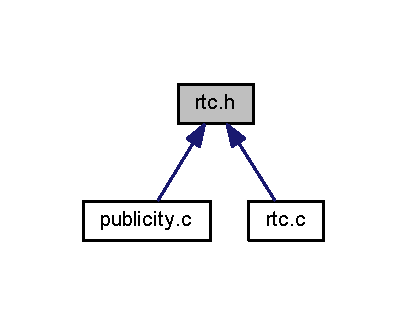
\includegraphics[width=196pt]{rtc_8h__dep__incl}
\end{center}
\end{figure}
\subsection*{Data Structures}
\begin{DoxyCompactItemize}
\item 
struct \hyperlink{structdate__t}{date\+\_\+t}
\end{DoxyCompactItemize}
\subsection*{Macros}
\begin{Indent}{\bf R\+TC M\+A\+C\+R\+OS}\par
\begin{DoxyCompactItemize}
\item 
\#define \hyperlink{group__rtc_ga710b98232df2c563009e6f8a6cd18220}{R\+T\+C\+\_\+\+A\+D\+D\+R\+\_\+\+R\+EG}~0x70
\item 
\#define \hyperlink{group__rtc_ga2f258a00c59c3f347c8d2d4a75471ce0}{R\+T\+C\+\_\+\+D\+A\+T\+A\+\_\+\+R\+EG}~0x71
\item 
\#define \hyperlink{group__rtc_ga4e22feb6ffbc1cda32fadff5c740dc51}{R\+T\+C\+\_\+\+I\+RQ}~8
\end{DoxyCompactItemize}
\end{Indent}
\subsection*{Functions}
\begin{DoxyCompactItemize}
\item 
int \hyperlink{group__rtc_ga3b9f4583bad77c33ea0e82c1c1ad5305}{rtc\+\_\+subscribe\+\_\+int} (unsigned int $\ast$rtc\+\_\+hook\+\_\+id)
\begin{DoxyCompactList}\small\item\em subscribes a R\+TC interruption \end{DoxyCompactList}\item 
int \hyperlink{group__rtc_ga61932ec1f55303bac55dea276d2a141f}{rtc\+\_\+unsubscribe\+\_\+int} (unsigned int $\ast$rtc\+\_\+hook\+\_\+id)
\begin{DoxyCompactList}\small\item\em unsubscribes a R\+TC interruption \end{DoxyCompactList}\item 
int \hyperlink{group__rtc_ga9a66dc15a321b825a97887478a95e28f}{rtc\+\_\+read} (unsigned int reg, unsigned int $\ast$inf)
\begin{DoxyCompactList}\small\item\em reads from the rtc \end{DoxyCompactList}\item 
int \hyperlink{group__rtc_ga83dbab748017bcc8531622b94cca1be1}{rtc\+\_\+read\+\_\+date} (\hyperlink{structdate__t}{date\+\_\+t} $\ast$date)
\begin{DoxyCompactList}\small\item\em gets the date from the rtc \end{DoxyCompactList}\end{DoxyCompactItemize}

\hypertarget{ser__port_8c}{}\section{ser\+\_\+port.\+c File Reference}
\label{ser__port_8c}\index{ser\+\_\+port.\+c@{ser\+\_\+port.\+c}}
{\ttfamily \#include $<$minix/syslib.\+h$>$}\newline
{\ttfamily \#include $<$minix/drivers.\+h$>$}\newline
{\ttfamily \#include $<$minix/sysutil.\+h$>$}\newline
{\ttfamily \#include \char`\"{}ser\+\_\+port.\+h\char`\"{}}\newline
Include dependency graph for ser\+\_\+port.\+c\+:
\nopagebreak
\begin{figure}[H]
\begin{center}
\leavevmode
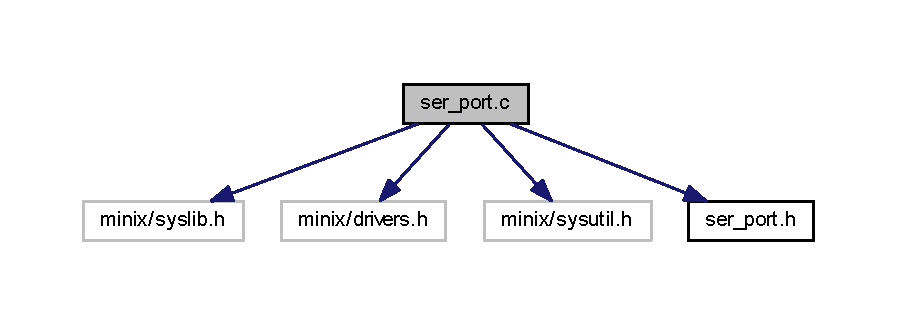
\includegraphics[width=350pt]{ser__port_8c__incl}
\end{center}
\end{figure}
\subsection*{Functions}
\begin{DoxyCompactItemize}
\item 
\hyperlink{structser__conf__t}{ser\+\_\+conf\+\_\+t} \hyperlink{group__ser__port_gad7f306574426f807f460ddcde260c11b}{get\+\_\+conf} (unsigned short base\+\_\+addr)
\begin{DoxyCompactList}\small\item\em This function gets the configuration of an U\+A\+RT register. \end{DoxyCompactList}\item 
int \hyperlink{group__ser__port_ga03bc33099d89326fb9a26cc0fef1cc7a}{ser\+\_\+set\+\_\+bits\+\_\+per\+\_\+char} (unsigned short base\+\_\+addr, int bits)
\begin{DoxyCompactList}\small\item\em Sets the value of bits per character in the respective serial port. \end{DoxyCompactList}\item 
int \hyperlink{group__ser__port_ga7d67a8d80697182bb1afe90a65875c90}{ser\+\_\+set\+\_\+stop\+\_\+bits} (unsigned short base\+\_\+addr, int bits)
\begin{DoxyCompactList}\small\item\em Sets the value of bits per character in the respective serial port. \end{DoxyCompactList}\item 
int \hyperlink{group__ser__port_ga4a963c8e3cfb978a4e4a026add12483f}{ser\+\_\+set\+\_\+parity} (unsigned short base\+\_\+addr, int parity)
\begin{DoxyCompactList}\small\item\em Sets the value of bits per character in the respective serial port. \end{DoxyCompactList}\item 
int \hyperlink{group__ser__port_ga2b6153e7105a706ea7a331770150ac55}{ser\+\_\+set\+\_\+rate} (unsigned short base\+\_\+addr, int rate)
\begin{DoxyCompactList}\small\item\em Sets the value of bits per character in the respective serial port. \end{DoxyCompactList}\item 
int \hyperlink{group__ser__port_ga1e0894432789b7311021c4f862335065}{ser\+\_\+set\+\_\+conf} (unsigned short base\+\_\+addr, int bits, int stop, int parity, int rate)
\begin{DoxyCompactList}\small\item\em Sets the configuration of the serial port. \end{DoxyCompactList}\item 
int \hyperlink{group__ser__port_gaf51d56fa6069ce68bb9f34a1396b2ea1}{ser\+\_\+check\+\_\+lsr\+\_\+error} (unsigned short base\+\_\+addr)
\begin{DoxyCompactList}\small\item\em Checks if the lsr register has an error. \end{DoxyCompactList}\item 
int \hyperlink{group__ser__port_ga46bbb861095c5b7a44a33af5e19be100}{ser\+\_\+disable\+\_\+int} (unsigned short base\+\_\+addr)
\begin{DoxyCompactList}\small\item\em Disables I\+ER interrupts. \end{DoxyCompactList}\item 
int \hyperlink{group__ser__port_gae9c2959fb0c4f39b96c4621d985f5ed2}{ser\+\_\+receive\+\_\+char\+\_\+poll} (unsigned short base\+\_\+addr, unsigned long $\ast$c, int num\+\_\+cicles)
\begin{DoxyCompactList}\small\item\em receive a char through the serial port \end{DoxyCompactList}\item 
int \hyperlink{group__ser__port_ga9ce4605b9346d093f446fa48b495406b}{ser\+\_\+send\+\_\+char\+\_\+poll} (unsigned short base\+\_\+addr, char c, int num\+\_\+cicles)
\begin{DoxyCompactList}\small\item\em transmits a char through the serial port \end{DoxyCompactList}\end{DoxyCompactItemize}

\hypertarget{ser__port_8h}{}\section{ser\+\_\+port.\+h File Reference}
\label{ser__port_8h}\index{ser\+\_\+port.\+h@{ser\+\_\+port.\+h}}
This graph shows which files directly or indirectly include this file\+:
\nopagebreak
\begin{figure}[H]
\begin{center}
\leavevmode
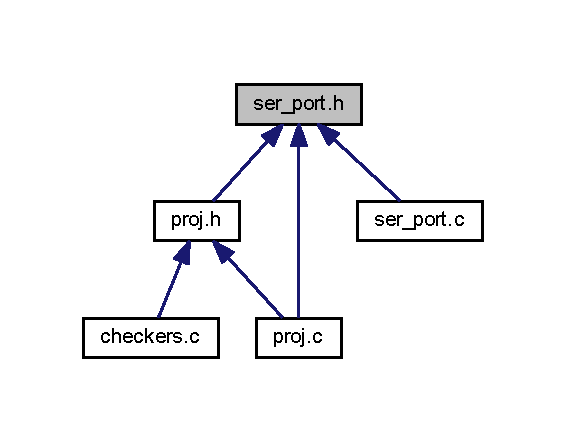
\includegraphics[width=272pt]{ser__port_8h__dep__incl}
\end{center}
\end{figure}
\subsection*{Data Structures}
\begin{DoxyCompactItemize}
\item 
struct \hyperlink{structser__conf__t}{ser\+\_\+conf\+\_\+t}
\end{DoxyCompactItemize}
\subsection*{Macros}
\begin{DoxyCompactItemize}
\item 
\#define \hyperlink{group__ser__port_ga3a8ea58898cb58fc96013383d39f482c}{B\+IT}(n)~(0x01$<$$<$(n))
\item 
\#define \hyperlink{group__ser__port_ga98199cd85fbe47b9a741b07762260422}{S\+E\+R\+\_\+\+C\+O\+M1\+\_\+\+A\+D\+DR}~0x3\+F8
\item 
\#define \hyperlink{group__ser__port_ga62c7a28d9eaa93631e7bb202f91dddcf}{S\+E\+R\+\_\+\+C\+O\+M2\+\_\+\+A\+D\+DR}~0x2\+F8
\item 
\#define \hyperlink{group__ser__port_gaf0ec610995d060379690114f01c6eeaf}{S\+E\+R\+\_\+\+C\+O\+M1\+\_\+\+I\+RQ}~4
\item 
\#define \hyperlink{group__ser__port_ga420c631d8b538f2a8058e793523149e2}{S\+E\+R\+\_\+\+C\+O\+M2\+\_\+\+I\+RQ}~3
\item 
\#define \hyperlink{group__ser__port_ga673bc80505f70c750fe685caf9a0d6b0}{S\+E\+R\+\_\+\+H\+O\+OK}~5
\item 
\#define \hyperlink{group__ser__port_ga1a522aa19bcb695a9df30032a893bee3}{D\+E\+L\+A\+Y\+\_\+\+US}~20000
\end{DoxyCompactItemize}
\begin{Indent}{\bf R\+E\+G\+I\+S\+T\+ER}\par
\begin{DoxyCompactItemize}
\item 
\#define \hyperlink{group__ser__port_gaab10abea0297abdcf0aab7d7d0b5662f}{S\+E\+R\+\_\+\+R\+BR}~0
\item 
\#define \hyperlink{group__ser__port_ga3702c28928f73b9841ab8269f64177ed}{S\+E\+R\+\_\+\+T\+HR}~0
\item 
\#define \hyperlink{group__ser__port_ga783f8e3973a5f87d8af120d49742f834}{S\+E\+R\+\_\+\+I\+ER}~1
\item 
\#define \hyperlink{group__ser__port_ga483c46ea5ed36388947426211cb63eab}{S\+E\+R\+\_\+\+I\+IR}~2
\item 
\#define \hyperlink{group__ser__port_ga9261eef6859842b51e42894b61c5b1c0}{S\+E\+R\+\_\+\+F\+CR}~2
\item 
\#define \hyperlink{group__ser__port_ga6475db6ed9440a92c680e54b2912b191}{S\+E\+R\+\_\+\+L\+CR}~3
\item 
\#define \hyperlink{group__ser__port_ga0f21de7866d73161df9b492b415c370c}{S\+E\+R\+\_\+\+M\+CR}~4
\item 
\#define \hyperlink{group__ser__port_ga382b5d26eb113bfffbf2094eb4405042}{S\+E\+R\+\_\+\+L\+SR}~5
\item 
\#define \hyperlink{group__ser__port_gaf161670921d63a654492758b1998d222}{S\+E\+R\+\_\+\+M\+SR}~6
\item 
\#define \hyperlink{group__ser__port_ga0005836362c1dd009c7fe47720908b1b}{S\+E\+R\+\_\+\+SR}~7
\item 
\#define \hyperlink{group__ser__port_ga858484a29128b93600cd6b8971a91faf}{S\+E\+R\+\_\+\+D\+LL}~0
\item 
\#define \hyperlink{group__ser__port_ga54c2d9bcb790f3a6d0cd71d20ae5d427}{S\+E\+R\+\_\+\+D\+LM}~1
\item 
\#define \hyperlink{group__ser__port_ga2bce41e3ef0b59643bfc314fbdf89545}{S\+E\+R\+\_\+\+D\+L\+AB}~\hyperlink{video__gr_8c_a3a8ea58898cb58fc96013383d39f482c}{B\+IT}(7)
\end{DoxyCompactItemize}
\end{Indent}
\begin{Indent}{\bf S\+ER D\+A\+TA}\par
\begin{DoxyCompactItemize}
\item 
\#define \hyperlink{group__ser__port_gadf09d6c9cf68d22c596eb240a5febffb}{S\+E\+R\+\_\+\+D\+A\+TA}~0
\item 
\#define \hyperlink{group__ser__port_ga39627267c307802e2a030abe796fb97b}{S\+E\+R\+\_\+\+T\+X\+\_\+\+R\+DY}~(1$<$$<$5)
\item 
\#define \hyperlink{group__ser__port_ga3eb8525f2a4c6e405b2528526c71b0cf}{S\+E\+R\+\_\+\+R\+E\+C\+\_\+\+R\+DY}~\hyperlink{video__gr_8c_a3a8ea58898cb58fc96013383d39f482c}{B\+IT}(0)
\end{DoxyCompactItemize}
\end{Indent}
\begin{Indent}{\bf I\+ER}\par
\begin{DoxyCompactItemize}
\item 
\#define \hyperlink{group__ser__port_gafe8e1c08ba9763a976c8359d6f5b370b}{E\+N\+A\+B\+L\+E\+\_\+\+R\+E\+C\+\_\+\+I\+NT}~\hyperlink{video__gr_8c_a3a8ea58898cb58fc96013383d39f482c}{B\+IT}(0)
\item 
\#define \hyperlink{group__ser__port_gac33182192c6023fe0d50c63666551162}{E\+N\+A\+B\+L\+E\+\_\+\+T\+R\+A\+N\+S\+\_\+\+I\+NT}~\hyperlink{video__gr_8c_a3a8ea58898cb58fc96013383d39f482c}{B\+IT}(1)
\item 
\#define \hyperlink{group__ser__port_ga89361f04d2aef788b076d1ea455d5482}{E\+N\+A\+B\+L\+E\+\_\+\+L\+I\+N\+E\+\_\+\+S\+T\+A\+T\+U\+S\+\_\+\+I\+NT}~\hyperlink{video__gr_8c_a3a8ea58898cb58fc96013383d39f482c}{B\+IT}(2)
\end{DoxyCompactItemize}
\end{Indent}
\begin{Indent}{\bf E\+R\+R\+OR}\par
\begin{DoxyCompactItemize}
\item 
\#define \hyperlink{group__ser__port_gac22f7e8109686500cf878a26ea3af115}{S\+E\+R\+\_\+\+O\+V\+E\+R\+R\+U\+N\+\_\+\+E\+RR}~(1$<$$<$1)
\item 
\#define \hyperlink{group__ser__port_ga356ae2e9093b65d87b35a303f3092057}{S\+E\+R\+\_\+\+P\+A\+R\+I\+T\+Y\+\_\+\+E\+RR}~(1$<$$<$2)
\item 
\#define \hyperlink{group__ser__port_ga0182fcdfbfeb90906d60c3ddb411aece}{S\+E\+R\+\_\+\+F\+R\+A\+M\+E\+\_\+\+E\+RR}~(1$<$$<$3)
\end{DoxyCompactItemize}
\end{Indent}
\begin{Indent}{\bf F\+I\+FO}\par
\begin{DoxyCompactItemize}
\item 
\#define \hyperlink{group__ser__port_ga096773e56aa66b4b8721492e07c41c77}{S\+E\+R\+\_\+\+E\+N\+\_\+\+F\+I\+FO}~\hyperlink{video__gr_8c_a3a8ea58898cb58fc96013383d39f482c}{B\+IT}(0)
\item 
\#define \hyperlink{group__ser__port_ga3b73c7fc2c9e1534d663a7b8c588240a}{S\+E\+R\+\_\+\+C\+L\+R\+\_\+\+R\+E\+C\+\_\+\+F\+I\+FO}~\hyperlink{video__gr_8c_a3a8ea58898cb58fc96013383d39f482c}{B\+IT}(1)
\item 
\#define \hyperlink{group__ser__port_ga565f202296c0e98389a04cf981110b2a}{S\+E\+R\+\_\+\+C\+L\+R\+\_\+\+T\+R\+A\+N\+S\+\_\+\+F\+I\+FO}~\hyperlink{video__gr_8c_a3a8ea58898cb58fc96013383d39f482c}{B\+IT}(2)
\item 
\#define \hyperlink{group__ser__port_ga4c5703803ba2f88b2c80a98503cd7b48}{S\+E\+R\+\_\+\+T\+R\+I\+G\+G\+ER}~\hyperlink{video__gr_8c_a3a8ea58898cb58fc96013383d39f482c}{B\+IT}(7)
\end{DoxyCompactItemize}
\end{Indent}
\begin{Indent}{\bf I\+IR}\par
\begin{DoxyCompactItemize}
\item 
\#define \hyperlink{group__ser__port_ga92820a610e36c919d8a8cb2bb731e43e}{S\+E\+R\+\_\+\+I\+N\+T\+\_\+\+O\+RG}~\hyperlink{video__gr_8c_a3a8ea58898cb58fc96013383d39f482c}{B\+IT}(3) $\vert$ \hyperlink{video__gr_8c_a3a8ea58898cb58fc96013383d39f482c}{B\+IT}(2) $\vert$\hyperlink{video__gr_8c_a3a8ea58898cb58fc96013383d39f482c}{B\+IT}(1)
\item 
\#define \hyperlink{group__ser__port_ga7685f0a713a489943c06459e830d7a86}{S\+E\+R\+\_\+\+I\+N\+T\+\_\+\+S\+T\+A\+T\+US}~\hyperlink{video__gr_8c_a3a8ea58898cb58fc96013383d39f482c}{B\+IT}(0)
\item 
\#define \hyperlink{group__ser__port_ga9cc69bb601e83e6539168370d49c71a5}{S\+E\+R\+\_\+\+I\+N\+T\+\_\+\+L\+I\+N\+E\+\_\+\+S\+T\+A\+T\+US}~(\hyperlink{video__gr_8c_a3a8ea58898cb58fc96013383d39f482c}{B\+IT}(2) $\vert$\hyperlink{video__gr_8c_a3a8ea58898cb58fc96013383d39f482c}{B\+IT}(1))
\item 
\#define \hyperlink{group__ser__port_gaa9a2bde6c86a448c7e5b3f2abd691da7}{S\+E\+R\+\_\+\+I\+N\+T\+\_\+\+T\+R\+A\+N\+S\+\_\+\+E\+M\+P\+TY}~\hyperlink{video__gr_8c_a3a8ea58898cb58fc96013383d39f482c}{B\+IT}(1)
\item 
\#define \hyperlink{group__ser__port_gad3a9fdeed634179f19f0fb175150faab}{S\+E\+R\+\_\+\+I\+N\+T\+\_\+\+R\+E\+C\+\_\+\+D\+A\+T\+A\+\_\+\+A\+V\+LB}~\hyperlink{video__gr_8c_a3a8ea58898cb58fc96013383d39f482c}{B\+IT}(2)
\end{DoxyCompactItemize}
\end{Indent}
\subsection*{Functions}
\begin{DoxyCompactItemize}
\item 
\hyperlink{structser__conf__t}{ser\+\_\+conf\+\_\+t} \hyperlink{group__ser__port_gad7f306574426f807f460ddcde260c11b}{get\+\_\+conf} (unsigned short base\+\_\+addr)
\begin{DoxyCompactList}\small\item\em This function gets the configuration of an U\+A\+RT register. \end{DoxyCompactList}\item 
int \hyperlink{group__ser__port_ga03bc33099d89326fb9a26cc0fef1cc7a}{ser\+\_\+set\+\_\+bits\+\_\+per\+\_\+char} (unsigned short base\+\_\+addr, int bits)
\begin{DoxyCompactList}\small\item\em Sets the value of bits per character in the respective serial port. \end{DoxyCompactList}\item 
int \hyperlink{group__ser__port_ga7d67a8d80697182bb1afe90a65875c90}{ser\+\_\+set\+\_\+stop\+\_\+bits} (unsigned short base\+\_\+addr, int bits)
\begin{DoxyCompactList}\small\item\em Sets the value of bits per character in the respective serial port. \end{DoxyCompactList}\item 
int \hyperlink{group__ser__port_ga4a963c8e3cfb978a4e4a026add12483f}{ser\+\_\+set\+\_\+parity} (unsigned short base\+\_\+addr, int parity)
\begin{DoxyCompactList}\small\item\em Sets the value of bits per character in the respective serial port. \end{DoxyCompactList}\item 
int \hyperlink{group__ser__port_ga2b6153e7105a706ea7a331770150ac55}{ser\+\_\+set\+\_\+rate} (unsigned short base\+\_\+addr, int rate)
\begin{DoxyCompactList}\small\item\em Sets the value of bits per character in the respective serial port. \end{DoxyCompactList}\item 
int \hyperlink{group__ser__port_ga1e0894432789b7311021c4f862335065}{ser\+\_\+set\+\_\+conf} (unsigned short base\+\_\+addr, int bits, int stop, int parity, int rate)
\begin{DoxyCompactList}\small\item\em Sets the configuration of the serial port. \end{DoxyCompactList}\item 
int \hyperlink{group__ser__port_gaf51d56fa6069ce68bb9f34a1396b2ea1}{ser\+\_\+check\+\_\+lsr\+\_\+error} (unsigned short base\+\_\+addr)
\begin{DoxyCompactList}\small\item\em Checks if the lsr register has an error. \end{DoxyCompactList}\item 
int \hyperlink{group__ser__port_ga46bbb861095c5b7a44a33af5e19be100}{ser\+\_\+disable\+\_\+int} (unsigned short base\+\_\+addr)
\begin{DoxyCompactList}\small\item\em Disables I\+ER interrupts. \end{DoxyCompactList}\item 
int \hyperlink{group__ser__port_ga9ce4605b9346d093f446fa48b495406b}{ser\+\_\+send\+\_\+char\+\_\+poll} (unsigned short base\+\_\+addr, char c, int num\+\_\+cicles)
\begin{DoxyCompactList}\small\item\em transmits a char through the serial port \end{DoxyCompactList}\item 
int \hyperlink{group__ser__port_gae9c2959fb0c4f39b96c4621d985f5ed2}{ser\+\_\+receive\+\_\+char\+\_\+poll} (unsigned short base\+\_\+addr, unsigned long $\ast$c, int num\+\_\+cicles)
\begin{DoxyCompactList}\small\item\em receive a char through the serial port \end{DoxyCompactList}\end{DoxyCompactItemize}

\hypertarget{timer_8c}{}\section{timer.\+c File Reference}
\label{timer_8c}\index{timer.\+c@{timer.\+c}}
{\ttfamily \#include \char`\"{}timer.\+h\char`\"{}}\newline
{\ttfamily \#include $<$minix/syslib.\+h$>$}\newline
{\ttfamily \#include $<$minix/drivers.\+h$>$}\newline
{\ttfamily \#include $<$minix/sysutil.\+h$>$}\newline
{\ttfamily \#include \char`\"{}utilities.\+h\char`\"{}}\newline
{\ttfamily \#include \char`\"{}i8042.\+h\char`\"{}}\newline
{\ttfamily \#include \char`\"{}i8254.\+h\char`\"{}}\newline
Include dependency graph for timer.\+c\+:
\nopagebreak
\begin{figure}[H]
\begin{center}
\leavevmode
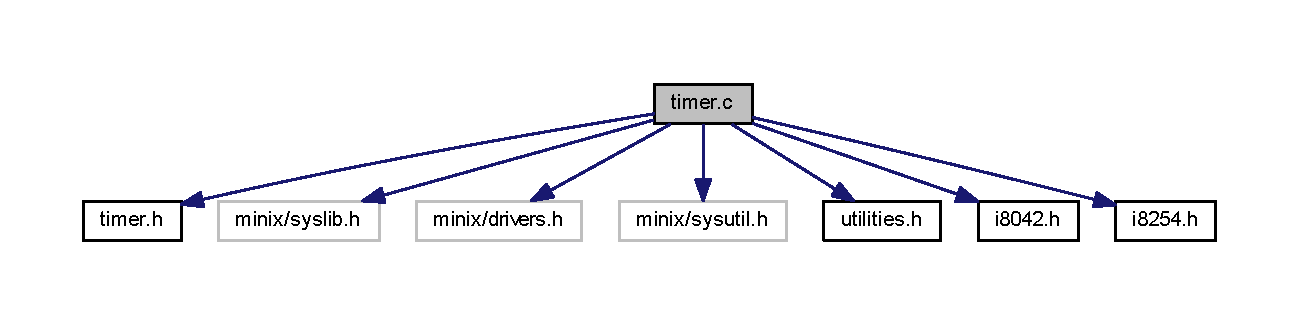
\includegraphics[width=350pt]{timer_8c__incl}
\end{center}
\end{figure}
\subsection*{Functions}
\begin{DoxyCompactItemize}
\item 
void \hyperlink{group__timer_ga05c1893c9a1e24ff5d76b2958adb8851}{ignore\+\_\+interrupts} (unsigned char hook)
\item 
int \hyperlink{group__timer_ga915070da84f7a3baa2e0fe634cb4bcd8}{timer\+\_\+subscribe\+\_\+int} (void)
\begin{DoxyCompactList}\small\item\em subscribes a timer interruption \end{DoxyCompactList}\item 
int \hyperlink{group__timer_gab9eea51549744bca5c5c923b388bb4ee}{timer\+\_\+unsubscribe\+\_\+int} ()
\begin{DoxyCompactList}\small\item\em unsubscribes a timer interruption \end{DoxyCompactList}\item 
int \hyperlink{group__timer_gada4efbb5c88275795526fc45f0814aa3}{timer\+\_\+set\+\_\+square} (unsigned long timer, unsigned long freq)
\begin{DoxyCompactList}\small\item\em sets the timer frequency \end{DoxyCompactList}\item 
int \hyperlink{group__timer_ga8eb3357bc05265afc4bea5bbbb480a53}{timer\+\_\+get\+\_\+conf} (unsigned long timer, unsigned char $\ast$st)
\begin{DoxyCompactList}\small\item\em Reads the input timer configuration via read-\/back command. \end{DoxyCompactList}\end{DoxyCompactItemize}
\subsection*{Variables}
\begin{DoxyCompactItemize}
\item 
int \hyperlink{timer_8c_a96e6321e488d93a8134897510c435eb7}{timer\+\_\+hook\+\_\+id} =0
\end{DoxyCompactItemize}


\subsection{Variable Documentation}
\hypertarget{timer_8c_a96e6321e488d93a8134897510c435eb7}{}\label{timer_8c_a96e6321e488d93a8134897510c435eb7} 
\index{timer.\+c@{timer.\+c}!timer\+\_\+hook\+\_\+id@{timer\+\_\+hook\+\_\+id}}
\index{timer\+\_\+hook\+\_\+id@{timer\+\_\+hook\+\_\+id}!timer.\+c@{timer.\+c}}
\subsubsection{\texorpdfstring{timer\+\_\+hook\+\_\+id}{timer\_hook\_id}}
{\footnotesize\ttfamily int timer\+\_\+hook\+\_\+id =0}


\hypertarget{timer_8h}{}\section{timer.\+h File Reference}
\label{timer_8h}\index{timer.\+h@{timer.\+h}}
This graph shows which files directly or indirectly include this file\+:
\nopagebreak
\begin{figure}[H]
\begin{center}
\leavevmode
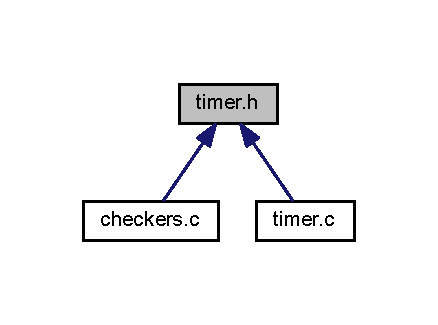
\includegraphics[width=210pt]{timer_8h__dep__incl}
\end{center}
\end{figure}
\subsection*{Functions}
\begin{DoxyCompactItemize}
\item 
void \hyperlink{group__timer_ga05c1893c9a1e24ff5d76b2958adb8851}{ignore\+\_\+interrupts} (unsigned char hook\+\_\+id)
\item 
int \hyperlink{group__timer_ga915070da84f7a3baa2e0fe634cb4bcd8}{timer\+\_\+subscribe\+\_\+int} ()
\begin{DoxyCompactList}\small\item\em subscribes a timer interruption \end{DoxyCompactList}\item 
int \hyperlink{group__timer_gab9eea51549744bca5c5c923b388bb4ee}{timer\+\_\+unsubscribe\+\_\+int} ()
\begin{DoxyCompactList}\small\item\em unsubscribes a timer interruption \end{DoxyCompactList}\item 
int \hyperlink{group__timer_gada4efbb5c88275795526fc45f0814aa3}{timer\+\_\+set\+\_\+square} (unsigned long timer, unsigned long freq)
\begin{DoxyCompactList}\small\item\em sets the timer frequency \end{DoxyCompactList}\item 
int \hyperlink{group__timer_ga8eb3357bc05265afc4bea5bbbb480a53}{timer\+\_\+get\+\_\+conf} (unsigned long timer, unsigned char $\ast$st)
\begin{DoxyCompactList}\small\item\em Reads the input timer configuration via read-\/back command. \end{DoxyCompactList}\end{DoxyCompactItemize}
\subsection*{Variables}
\begin{DoxyCompactItemize}
\item 
int \hyperlink{group__timer_ga96e6321e488d93a8134897510c435eb7}{timer\+\_\+hook\+\_\+id}
\begin{DoxyCompactList}\small\item\em hook for handling timer interruptions \end{DoxyCompactList}\end{DoxyCompactItemize}

\hypertarget{utilities_8c}{}\section{utilities.\+c File Reference}
\label{utilities_8c}\index{utilities.\+c@{utilities.\+c}}
{\ttfamily \#include \char`\"{}utilities.\+h\char`\"{}}\newline
Include dependency graph for utilities.\+c\+:
\nopagebreak
\begin{figure}[H]
\begin{center}
\leavevmode
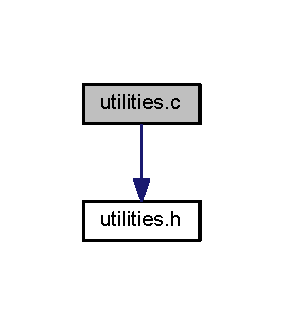
\includegraphics[width=136pt]{utilities_8c__incl}
\end{center}
\end{figure}
\subsection*{Functions}
\begin{DoxyCompactItemize}
\item 
void \hyperlink{group__utilities_gaf3cb5100a651058103311c52a27b4105}{stringcpy} (char $\ast$dest, char $\ast$src)
\item 
void \hyperlink{group__utilities_ga971bb40926a0f370263e085d1e2ac690}{stringcat} (char $\ast$dest, char $\ast$src)
\item 
int \hyperlink{group__utilities_gaa662bd9797d0cdd2707c9ad14849be44}{hex\+\_\+to\+\_\+dec} (int x)
\begin{DoxyCompactList}\small\item\em converts a number from hexadecimal to decimal \end{DoxyCompactList}\item 
int \hyperlink{group__utilities_ga529fd7b4e2b2f87cec4a30c191673207}{floor2} (double x)
\begin{DoxyCompactList}\small\item\em returns the floor of a double \end{DoxyCompactList}\item 
int \hyperlink{group__utilities_ga35abf8e6bc22bc3736fbd65416d8c3a2}{round} (double x)
\begin{DoxyCompactList}\small\item\em rounds x to the closest integer for example (9.\+5-\/$>$10; 9.\+45-\/$>$9) \end{DoxyCompactList}\item 
int \hyperlink{group__utilities_gafd4f329c8efb45c0dfff44525047a0fa}{abs} (int n)
\begin{DoxyCompactList}\small\item\em returns the absolute value of a number \end{DoxyCompactList}\item 
int \hyperlink{group__utilities_ga67452a3b663c47b61edb379f159ae478}{sgn} (int n)
\begin{DoxyCompactList}\small\item\em returns sign of a number \end{DoxyCompactList}\item 
int \hyperlink{group__utilities_ga92a937ad6b303c03cc98f5fe9354d235}{samesign} (int x, int y)
\begin{DoxyCompactList}\small\item\em checks if two number have the same sign \end{DoxyCompactList}\item 
int \hyperlink{group__utilities_ga75e5e4e3c99b54b12f0bb43becded2d1}{samesignarray} (int size, int $\ast$arr)
\begin{DoxyCompactList}\small\item\em checks if all the elements of an array have the same sign \end{DoxyCompactList}\item 
char \hyperlink{group__utilities_gac0df2a1416cd59f12dbc6adfd5f69ba3}{two\+\_\+complement\+\_\+sym} (char c)
\begin{DoxyCompactList}\small\item\em returns the opposite number in two complement to c \end{DoxyCompactList}\item 
int \hyperlink{group__utilities_ga79537e8684629d74571e64c633bb5303}{conv\+\_\+to\+\_\+decimal} (char c)
\begin{DoxyCompactList}\small\item\em converts a char to decimal \end{DoxyCompactList}\end{DoxyCompactItemize}

\hypertarget{utilities_8h}{}\section{utilities.\+h File Reference}
\label{utilities_8h}\index{utilities.\+h@{utilities.\+h}}
This graph shows which files directly or indirectly include this file\+:
\nopagebreak
\begin{figure}[H]
\begin{center}
\leavevmode
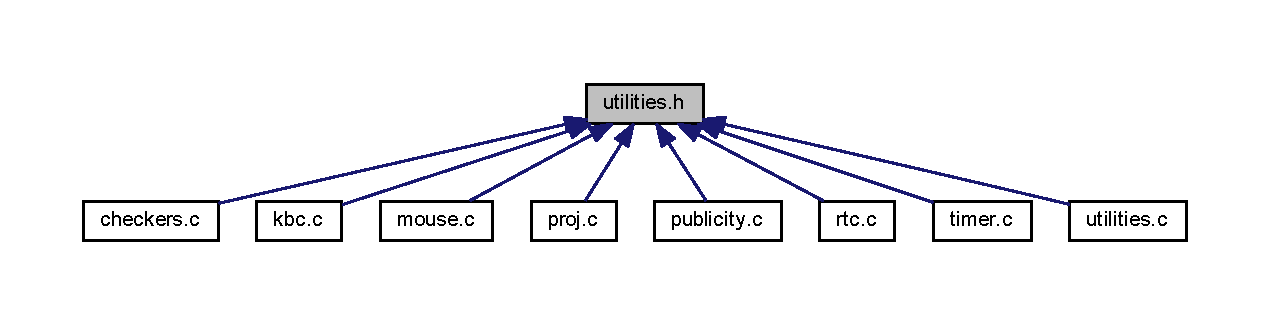
\includegraphics[width=350pt]{utilities_8h__dep__incl}
\end{center}
\end{figure}
\subsection*{Macros}
\begin{DoxyCompactItemize}
\item 
\#define \hyperlink{group__utilities_ga3a8ea58898cb58fc96013383d39f482c}{B\+IT}(n)~(0x01$<$$<$(n))
\item 
\#define \hyperlink{group__utilities_gab2e0399a4e6f9f5eb241bade77f59ea1}{I\+S\+\_\+\+B\+R\+E\+A\+K\+C\+O\+DE}(c)~(c$>$$>$7)
\item 
\#define \hyperlink{group__utilities_ga1a522aa19bcb695a9df30032a893bee3}{D\+E\+L\+A\+Y\+\_\+\+US}~20000
\end{DoxyCompactItemize}
\subsection*{Functions}
\begin{DoxyCompactItemize}
\item 
void \hyperlink{group__utilities_gaf3cb5100a651058103311c52a27b4105}{stringcpy} (char $\ast$dest, char $\ast$src)
\item 
void \hyperlink{group__utilities_ga971bb40926a0f370263e085d1e2ac690}{stringcat} (char $\ast$dest, char $\ast$src)
\item 
int \hyperlink{group__utilities_gaa662bd9797d0cdd2707c9ad14849be44}{hex\+\_\+to\+\_\+dec} (int x)
\begin{DoxyCompactList}\small\item\em converts a number from hexadecimal to decimal \end{DoxyCompactList}\item 
int \hyperlink{group__utilities_gafd4f329c8efb45c0dfff44525047a0fa}{abs} (int n)
\begin{DoxyCompactList}\small\item\em returns the absolute value of a number \end{DoxyCompactList}\item 
int \hyperlink{group__utilities_ga529fd7b4e2b2f87cec4a30c191673207}{floor2} (double x)
\begin{DoxyCompactList}\small\item\em returns the floor of a double \end{DoxyCompactList}\item 
int \hyperlink{group__utilities_ga35abf8e6bc22bc3736fbd65416d8c3a2}{round} (double x)
\begin{DoxyCompactList}\small\item\em rounds x to the closest integer for example (9.\+5-\/$>$10; 9.\+45-\/$>$9) \end{DoxyCompactList}\item 
int \hyperlink{group__utilities_ga67452a3b663c47b61edb379f159ae478}{sgn} (int n)
\begin{DoxyCompactList}\small\item\em returns sign of a number \end{DoxyCompactList}\item 
int \hyperlink{group__utilities_ga92a937ad6b303c03cc98f5fe9354d235}{samesign} (int x, int y)
\begin{DoxyCompactList}\small\item\em checks if two number have the same sign \end{DoxyCompactList}\item 
int \hyperlink{group__utilities_ga75e5e4e3c99b54b12f0bb43becded2d1}{samesignarray} (int size, int $\ast$arr)
\begin{DoxyCompactList}\small\item\em checks if all the elements of an array have the same sign \end{DoxyCompactList}\item 
char \hyperlink{group__utilities_gac0df2a1416cd59f12dbc6adfd5f69ba3}{two\+\_\+complement\+\_\+sym} (char c)
\begin{DoxyCompactList}\small\item\em returns the opposite number in two complement to c \end{DoxyCompactList}\item 
int \hyperlink{group__utilities_ga79537e8684629d74571e64c633bb5303}{conv\+\_\+to\+\_\+decimal} (char c)
\begin{DoxyCompactList}\small\item\em converts a char to decimal \end{DoxyCompactList}\end{DoxyCompactItemize}

\hypertarget{vbe_8c}{}\section{vbe.\+c File Reference}
\label{vbe_8c}\index{vbe.\+c@{vbe.\+c}}
{\ttfamily \#include $<$minix/syslib.\+h$>$}\newline
{\ttfamily \#include $<$minix/drivers.\+h$>$}\newline
{\ttfamily \#include $<$machine/int86.\+h$>$}\newline
{\ttfamily \#include \char`\"{}vbe.\+h\char`\"{}}\newline
{\ttfamily \#include \char`\"{}lmlib.\+h\char`\"{}}\newline
Include dependency graph for vbe.\+c\+:
\nopagebreak
\begin{figure}[H]
\begin{center}
\leavevmode
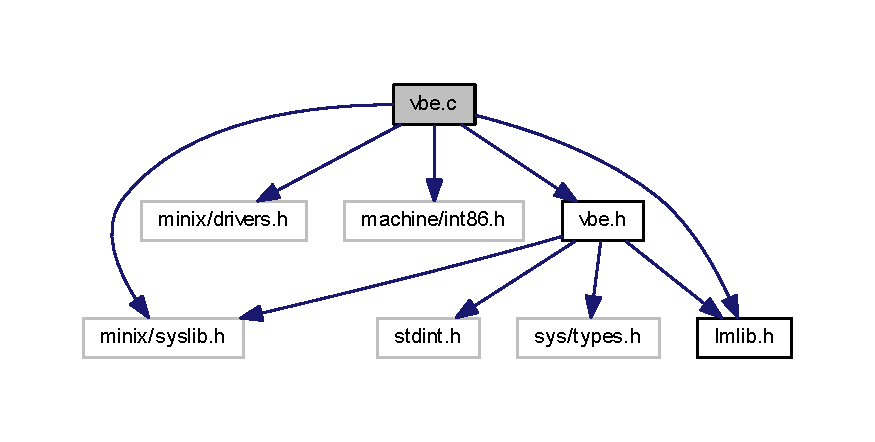
\includegraphics[width=350pt]{vbe_8c__incl}
\end{center}
\end{figure}
\subsection*{Macros}
\begin{DoxyCompactItemize}
\item 
\#define \hyperlink{vbe_8c_a68b87c2339cb305d66b69b5551b96c73}{P\+B2\+B\+A\+SE}(x)~(((x) $>$$>$ 4) \& 0x0\+F000)
\item 
\#define \hyperlink{vbe_8c_a70c65ed4c6d71865daa96d31befb33fd}{P\+B2\+O\+FF}(x)~((x) \& 0x0\+F\+F\+F\+F)
\end{DoxyCompactItemize}
\subsection*{Functions}
\begin{DoxyCompactItemize}
\item 
int \hyperlink{group__vbe_ga4ef3234e41f2050bc094a22049b69e45}{vbe\+\_\+get\+\_\+mode\+\_\+info} (unsigned short mode, \hyperlink{structvbe__mode__info__t}{vbe\+\_\+mode\+\_\+info\+\_\+t} $\ast$vmi\+\_\+p)
\begin{DoxyCompactList}\small\item\em Returns information on the input V\+BE mode, including screen dimensions, color depth and V\+R\+AM physical address. \end{DoxyCompactList}\item 
int \hyperlink{group__vbe_ga4e9da75c9063842b969ad400e5700c0c}{vbe\+\_\+get\+\_\+info\+\_\+block} (\hyperlink{structvbe__info__block__t}{vbe\+\_\+info\+\_\+block\+\_\+t} $\ast$vmi\+\_\+p)
\begin{DoxyCompactList}\small\item\em Returns information on the controller. \end{DoxyCompactList}\end{DoxyCompactItemize}


\subsection{Macro Definition Documentation}
\hypertarget{vbe_8c_a68b87c2339cb305d66b69b5551b96c73}{}\label{vbe_8c_a68b87c2339cb305d66b69b5551b96c73} 
\index{vbe.\+c@{vbe.\+c}!P\+B2\+B\+A\+SE@{P\+B2\+B\+A\+SE}}
\index{P\+B2\+B\+A\+SE@{P\+B2\+B\+A\+SE}!vbe.\+c@{vbe.\+c}}
\subsubsection{\texorpdfstring{P\+B2\+B\+A\+SE}{PB2BASE}}
{\footnotesize\ttfamily \#define P\+B2\+B\+A\+SE(\begin{DoxyParamCaption}\item[{}]{x }\end{DoxyParamCaption})~(((x) $>$$>$ 4) \& 0x0\+F000)}

\hypertarget{vbe_8c_a70c65ed4c6d71865daa96d31befb33fd}{}\label{vbe_8c_a70c65ed4c6d71865daa96d31befb33fd} 
\index{vbe.\+c@{vbe.\+c}!P\+B2\+O\+FF@{P\+B2\+O\+FF}}
\index{P\+B2\+O\+FF@{P\+B2\+O\+FF}!vbe.\+c@{vbe.\+c}}
\subsubsection{\texorpdfstring{P\+B2\+O\+FF}{PB2OFF}}
{\footnotesize\ttfamily \#define P\+B2\+O\+FF(\begin{DoxyParamCaption}\item[{}]{x }\end{DoxyParamCaption})~((x) \& 0x0\+F\+F\+F\+F)}


\hypertarget{vbe_8h}{}\section{vbe.\+h File Reference}
\label{vbe_8h}\index{vbe.\+h@{vbe.\+h}}
{\ttfamily \#include $<$stdint.\+h$>$}\newline
{\ttfamily \#include \char`\"{}lmlib.\+h\char`\"{}}\newline
{\ttfamily \#include $<$minix/syslib.\+h$>$}\newline
{\ttfamily \#include $<$sys/types.\+h$>$}\newline
Include dependency graph for vbe.\+h\+:
\nopagebreak
\begin{figure}[H]
\begin{center}
\leavevmode
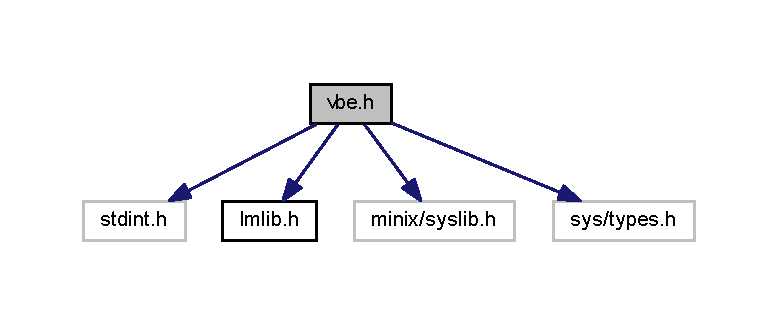
\includegraphics[width=350pt]{vbe_8h__incl}
\end{center}
\end{figure}
This graph shows which files directly or indirectly include this file\+:
\nopagebreak
\begin{figure}[H]
\begin{center}
\leavevmode
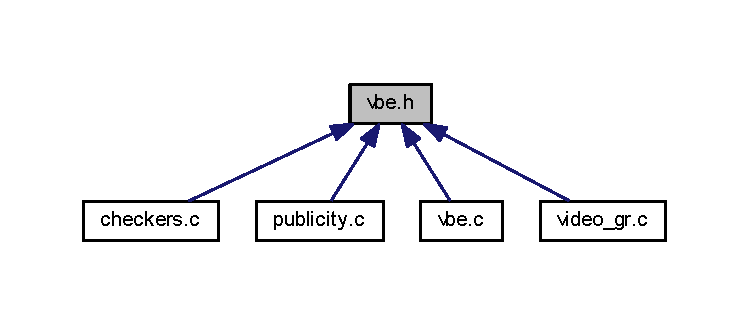
\includegraphics[width=350pt]{vbe_8h__dep__incl}
\end{center}
\end{figure}
\subsection*{Data Structures}
\begin{DoxyCompactItemize}
\item 
struct \hyperlink{structvbe__mode__info__t}{vbe\+\_\+mode\+\_\+info\+\_\+t}
\item 
struct \hyperlink{structvbe__info__block__t}{vbe\+\_\+info\+\_\+block\+\_\+t}
\end{DoxyCompactItemize}
\subsection*{Macros}
\begin{Indent}{\bf G\+E\+N\+E\+R\+IC M\+A\+C\+R\+OS}\par
\begin{DoxyCompactItemize}
\item 
\#define \hyperlink{group__vbe_ga68b87c2339cb305d66b69b5551b96c73}{P\+B2\+B\+A\+SE}(x)~(((x) $>$$>$ 4) \& 0x0\+F000)
\item 
\#define \hyperlink{group__vbe_ga70c65ed4c6d71865daa96d31befb33fd}{P\+B2\+O\+FF}(x)~((x) \& 0x0\+F\+F\+F\+F)
\item 
\#define \hyperlink{group__vbe_ga9cb0519a88e2860f94e49d7444ee5725}{V\+B\+E\+\_\+\+F\+U\+N\+C\+T\+I\+O\+N\+\_\+\+I\+N\+V\+O\+KE}~0x4F
\item 
\#define \hyperlink{group__vbe_ga13e1037464e7407d1df6aa4041b180cd}{V\+B\+E\+\_\+\+I\+N\+T\+E\+R\+R\+U\+PT}~0x10
\end{DoxyCompactItemize}
\end{Indent}
\begin{Indent}{\bf F\+U\+N\+C\+T\+I\+O\+NS}\par
\begin{DoxyCompactItemize}
\item 
\#define \hyperlink{group__vbe_ga7850c02defc99773b2704700c6cab3fd}{V\+B\+E\+\_\+\+R\+E\+T\+U\+R\+N\+\_\+\+C\+O\+N\+T\+R\+O\+L\+L\+ER}~0x00
\item 
\#define \hyperlink{group__vbe_gab9d80b9e6d7846ea3fa090c817771866}{V\+B\+E\+\_\+\+R\+E\+T\+U\+R\+N\+\_\+\+M\+O\+DE}~0x01
\item 
\#define \hyperlink{group__vbe_ga02477c4996ff058aee590b54f2146eb5}{V\+B\+E\+\_\+\+S\+E\+T\+\_\+\+M\+O\+DE}~0x02
\end{DoxyCompactItemize}
\end{Indent}
\begin{Indent}{\bf V\+BE R\+E\+T\+U\+RN S\+T\+A\+T\+US}\par
\begin{DoxyCompactItemize}
\item 
\#define \hyperlink{group__vbe_gaf48e8544d690af8d91d99653bad50a28}{V\+B\+E\+\_\+\+F\+U\+N\+C\+T\+I\+O\+N\+\_\+\+S\+U\+C\+C\+E\+SS}~0x00
\item 
\#define \hyperlink{group__vbe_ga0a4df98507b443e279641268d5583a3e}{V\+B\+E\+\_\+\+F\+U\+N\+C\+T\+I\+O\+N\+\_\+\+F\+A\+I\+L\+ED}~0x01
\item 
\#define \hyperlink{group__vbe_ga265850c04b2ec9164871c40cb8aa3b4f}{V\+B\+E\+\_\+\+F\+U\+N\+C\+T\+I\+O\+N\+\_\+\+N\+O\+T\+\_\+\+S\+U\+P\+P\+O\+R\+T\+ED}~0x02
\item 
\#define \hyperlink{group__vbe_ga48de88d26f563ed30a13e8158b90a54f}{V\+B\+E\+\_\+\+F\+U\+N\+C\+T\+I\+O\+N\+\_\+\+I\+N\+V\+A\+L\+ID}~0x03
\item 
\#define \hyperlink{group__vbe_ga4aba3d39cac7f9bc65f8b97a8daa88c6}{V\+B\+E\+\_\+\+F\+U\+N\+C\+T\+I\+O\+N\+\_\+\+S\+U\+P\+P\+O\+R\+T\+ED}~0x4F
\end{DoxyCompactItemize}
\end{Indent}
\begin{Indent}{\bf V\+BE M\+O\+D\+ES}\par
\begin{DoxyCompactItemize}
\item 
\#define \hyperlink{group__vbe_ga6d93a7fdde65a4c44c41cd0fae46a471}{V\+B\+E\+\_\+\+M\+O\+D\+E\+\_\+\+L\+I\+N\+E\+A\+R\+\_\+\+B\+IT}~14
\item 
\#define \hyperlink{group__vbe_gaa0cd0b74a86aa2dc9eb78017743d6f1a}{V\+B\+E\+\_\+\+G\+R\+A\+P\+H\+I\+C\+\_\+\+M\+O\+DE}~0x105
\item 
\#define \hyperlink{group__vbe_gac01942dc601c03d128c481824b1ae1d3}{V\+B\+E\+\_\+117\+\_\+\+M\+O\+DE}~0x117
\item 
\#define \hyperlink{group__vbe_gaf744f251b7e7d0acd6224997e46def7b}{V\+B\+E\+\_\+565\+\_\+\+M\+O\+DE}~0x11A
\end{DoxyCompactItemize}
\end{Indent}
\subsection*{Functions}
\begin{DoxyCompactItemize}
\item 
int \hyperlink{group__vbe_ga4ef3234e41f2050bc094a22049b69e45}{vbe\+\_\+get\+\_\+mode\+\_\+info} (unsigned short mode, \hyperlink{structvbe__mode__info__t}{vbe\+\_\+mode\+\_\+info\+\_\+t} $\ast$vmi\+\_\+p)
\begin{DoxyCompactList}\small\item\em Returns information on the input V\+BE mode, including screen dimensions, color depth and V\+R\+AM physical address. \end{DoxyCompactList}\item 
int \hyperlink{group__vbe_ga4e9da75c9063842b969ad400e5700c0c}{vbe\+\_\+get\+\_\+info\+\_\+block} (\hyperlink{structvbe__info__block__t}{vbe\+\_\+info\+\_\+block\+\_\+t} $\ast$vmi\+\_\+p)
\begin{DoxyCompactList}\small\item\em Returns information on the controller. \end{DoxyCompactList}\end{DoxyCompactItemize}

\hypertarget{video__gr_8c}{}\section{video\+\_\+gr.\+c File Reference}
\label{video__gr_8c}\index{video\+\_\+gr.\+c@{video\+\_\+gr.\+c}}
{\ttfamily \#include $<$minix/syslib.\+h$>$}\newline
{\ttfamily \#include $<$minix/drivers.\+h$>$}\newline
{\ttfamily \#include $<$machine/int86.\+h$>$}\newline
{\ttfamily \#include $<$sys/mman.\+h$>$}\newline
{\ttfamily \#include $<$sys/types.\+h$>$}\newline
{\ttfamily \#include $<$stdio.\+h$>$}\newline
{\ttfamily \#include \char`\"{}video\+\_\+gr.\+h\char`\"{}}\newline
{\ttfamily \#include \char`\"{}vbe.\+h\char`\"{}}\newline
Include dependency graph for video\+\_\+gr.\+c\+:
\nopagebreak
\begin{figure}[H]
\begin{center}
\leavevmode
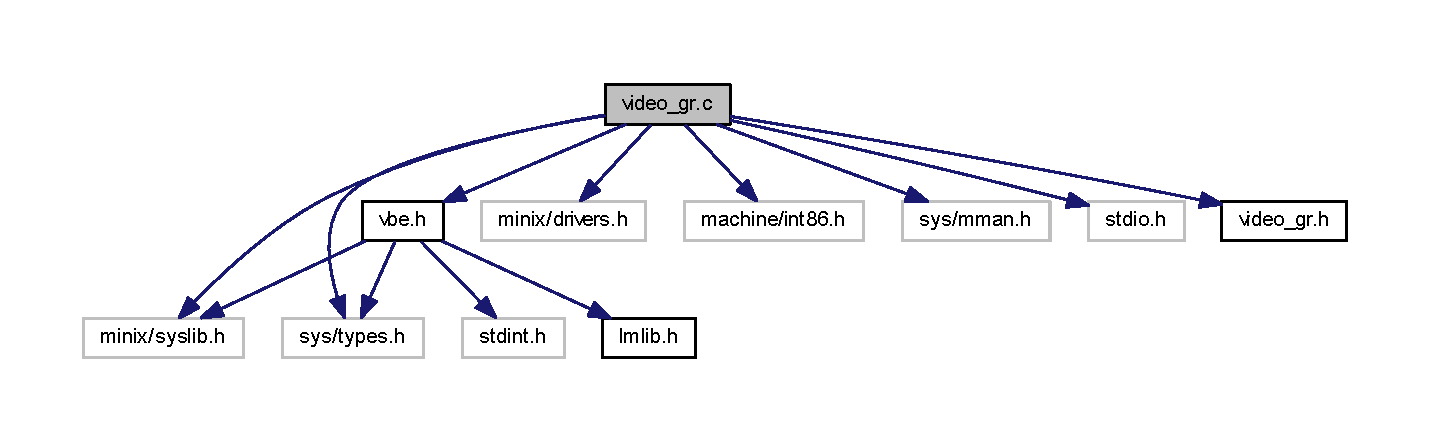
\includegraphics[width=350pt]{video__gr_8c__incl}
\end{center}
\end{figure}
\subsection*{Macros}
\begin{DoxyCompactItemize}
\item 
\#define \hyperlink{video__gr_8c_a3a8ea58898cb58fc96013383d39f482c}{B\+IT}(n)~(0x01$<$$<$(n))
\item 
\#define \hyperlink{video__gr_8c_ac854e8352d97c69bdfe247573593ba3b}{V\+R\+A\+M\+\_\+\+P\+H\+Y\+S\+\_\+\+A\+D\+DR}~0x\+F0000000
\item 
\#define \hyperlink{video__gr_8c_abf6f66114c31b8f87c80534ca695a00b}{H\+\_\+\+R\+ES}~1024
\item 
\#define \hyperlink{video__gr_8c_aac2466862bcfc18231c38fe1eacc22e3}{V\+\_\+\+R\+ES}~768
\item 
\#define \hyperlink{video__gr_8c_a35faf89171af20cd21088c37d62bb7ee}{B\+I\+T\+S\+\_\+\+P\+E\+R\+\_\+\+P\+I\+X\+EL}~8
\end{DoxyCompactItemize}
\subsection*{Functions}
\begin{DoxyCompactItemize}
\item 
unsigned \hyperlink{group__video__gr_ga80f6be1470280496d613f43fbf4f576c}{get\+Mouse\+\_\+buffer} ()
\begin{DoxyCompactList}\small\item\em gets pointer to variable mouse\+\_\+buffer \end{DoxyCompactList}\item 
unsigned \hyperlink{group__video__gr_gafa0e51016d7aa337778300ba2ec70a74}{get\+Double\+\_\+buffer} ()
\begin{DoxyCompactList}\small\item\em gets pointer to variable double\+\_\+buffer \end{DoxyCompactList}\item 
unsigned \hyperlink{video__gr_8c_adb4578dfdcaa8cbd0087cf160904a606}{get\+Video\+\_\+mem} ()
\item 
unsigned \hyperlink{group__video__gr_gaf597a67a797839097222fa9b4ae20b3f}{get\+H\+\_\+res} ()
\begin{DoxyCompactList}\small\item\em gets horizontal resolution of the screen \end{DoxyCompactList}\item 
unsigned \hyperlink{group__video__gr_ga36f1c43e43d903e085207548cf8d48a2}{get\+V\+\_\+res} ()
\begin{DoxyCompactList}\small\item\em gets vertical resolution of the screen \end{DoxyCompactList}\item 
int \hyperlink{group__video__gr_ga42f593e6656f1a978315aff02b1bcebf}{vg\+\_\+exit} ()
\begin{DoxyCompactList}\small\item\em Returns to default Minix 3 text mode (0x03\+: 25 x 80, 16 colors) \end{DoxyCompactList}\item 
void $\ast$ \hyperlink{group__video__gr_gacef21667c79365d57a084bed994c2189}{vg\+\_\+init} (unsigned short mode)
\begin{DoxyCompactList}\small\item\em Initializes the video module in graphics mode. \end{DoxyCompactList}\item 
int \hyperlink{group__video__gr_ga729c07175ab64956c7fd9944d7676888}{vg\+\_\+set\+\_\+pixel} (int x, int y, unsigned int color)
\begin{DoxyCompactList}\small\item\em sets the color of a pixel in the double buffer and in the mouse buffer \end{DoxyCompactList}\item 
int \hyperlink{group__video__gr_ga78765c3e4634b79d0c27b464be410803}{vg\+\_\+set\+\_\+mouse\+\_\+pixel} (int x, int y, unsigned int color)
\begin{DoxyCompactList}\small\item\em sets the color of a pixel in the mouse buffer \end{DoxyCompactList}\item 
int \hyperlink{group__video__gr_gafcdcee0785e2e5a0d0f1f460bf436403}{vg\+\_\+draw\+\_\+square} (int xi, int yi, int size, int color)
\begin{DoxyCompactList}\small\item\em draws a square in the double buffer and in the mouse buffer \end{DoxyCompactList}\item 
int \hyperlink{group__video__gr_ga0410a09b926582249fb7c0a795c9d4fe}{vg\+\_\+draw\+\_\+circle} (int xi, int yi, int radius, int color)
\begin{DoxyCompactList}\small\item\em draws a circle in the double buffer and in the mouse buffer \end{DoxyCompactList}\item 
int \hyperlink{group__video__gr_gae50eb47e283e71498d323e815411acc3}{swap\+\_\+double\+\_\+video} ()
\begin{DoxyCompactList}\small\item\em copies the double\+\_\+buffer into the video\+\_\+buffer \end{DoxyCompactList}\item 
int \hyperlink{group__video__gr_ga8761e145d6f2249e0a4177ed7ff24299}{swap\+\_\+mouse\+\_\+video} ()
\begin{DoxyCompactList}\small\item\em copies the mouse\+\_\+buffer into the video\+\_\+buffer \end{DoxyCompactList}\item 
int \hyperlink{group__video__gr_ga56155e15f2cbeb0c0790c3b22db43a78}{swap\+\_\+mouse\+\_\+double} ()
\begin{DoxyCompactList}\small\item\em copies the mouse\+\_\+buffer into the double\+\_\+buffer \end{DoxyCompactList}\item 
int \hyperlink{group__video__gr_gacbc2b21e05ad693bb6ed614f87329f05}{swap\+\_\+double\+\_\+mouse} ()
\begin{DoxyCompactList}\small\item\em copies the double\+\_\+buffer into the mouse\+\_\+buffer \end{DoxyCompactList}\item 
int \hyperlink{group__video__gr_gaeae89e446fefdba5e72413ff38727f44}{mouse\+\_\+to\+\_\+double} (int x, int y)
\begin{DoxyCompactList}\small\item\em sets a pixel in the mouse buffer to the color of the corresponding pixel in the double buffer \end{DoxyCompactList}\end{DoxyCompactItemize}
\subsection*{Variables}
\begin{DoxyCompactItemize}
\item 
static char $\ast$ \hyperlink{video__gr_8c_a93a24e067b9083bed6fb5c0336fd7a01}{video\+\_\+mem}
\item 
static char $\ast$ \hyperlink{video__gr_8c_a767d9dbba9c236b453eaaaf76976a6d0}{double\+\_\+buffer}
\item 
static char $\ast$ \hyperlink{video__gr_8c_a17f7fcbb13ae55b56a5d9e1b8859856c}{mouse\+\_\+buffer}
\item 
static unsigned \hyperlink{video__gr_8c_a43e7e5a0a8f9069e6413b2066ca52f3e}{h\+\_\+res}
\item 
static unsigned \hyperlink{video__gr_8c_a5bda1b499253a8fbf3cab646f8760391}{v\+\_\+res}
\item 
static unsigned \hyperlink{video__gr_8c_a89fa3fb58e975d148fcb2413e24b78a1}{bits\+\_\+per\+\_\+pixel}
\end{DoxyCompactItemize}


\subsection{Macro Definition Documentation}
\hypertarget{video__gr_8c_a3a8ea58898cb58fc96013383d39f482c}{}\label{video__gr_8c_a3a8ea58898cb58fc96013383d39f482c} 
\index{video\+\_\+gr.\+c@{video\+\_\+gr.\+c}!B\+IT@{B\+IT}}
\index{B\+IT@{B\+IT}!video\+\_\+gr.\+c@{video\+\_\+gr.\+c}}
\subsubsection{\texorpdfstring{B\+IT}{BIT}}
{\footnotesize\ttfamily \#define B\+IT(\begin{DoxyParamCaption}\item[{}]{n }\end{DoxyParamCaption})~(0x01$<$$<$(n))}

\hypertarget{video__gr_8c_a35faf89171af20cd21088c37d62bb7ee}{}\label{video__gr_8c_a35faf89171af20cd21088c37d62bb7ee} 
\index{video\+\_\+gr.\+c@{video\+\_\+gr.\+c}!B\+I\+T\+S\+\_\+\+P\+E\+R\+\_\+\+P\+I\+X\+EL@{B\+I\+T\+S\+\_\+\+P\+E\+R\+\_\+\+P\+I\+X\+EL}}
\index{B\+I\+T\+S\+\_\+\+P\+E\+R\+\_\+\+P\+I\+X\+EL@{B\+I\+T\+S\+\_\+\+P\+E\+R\+\_\+\+P\+I\+X\+EL}!video\+\_\+gr.\+c@{video\+\_\+gr.\+c}}
\subsubsection{\texorpdfstring{B\+I\+T\+S\+\_\+\+P\+E\+R\+\_\+\+P\+I\+X\+EL}{BITS\_PER\_PIXEL}}
{\footnotesize\ttfamily \#define B\+I\+T\+S\+\_\+\+P\+E\+R\+\_\+\+P\+I\+X\+EL~8}

\hypertarget{video__gr_8c_abf6f66114c31b8f87c80534ca695a00b}{}\label{video__gr_8c_abf6f66114c31b8f87c80534ca695a00b} 
\index{video\+\_\+gr.\+c@{video\+\_\+gr.\+c}!H\+\_\+\+R\+ES@{H\+\_\+\+R\+ES}}
\index{H\+\_\+\+R\+ES@{H\+\_\+\+R\+ES}!video\+\_\+gr.\+c@{video\+\_\+gr.\+c}}
\subsubsection{\texorpdfstring{H\+\_\+\+R\+ES}{H\_RES}}
{\footnotesize\ttfamily \#define H\+\_\+\+R\+ES~1024}

\hypertarget{video__gr_8c_aac2466862bcfc18231c38fe1eacc22e3}{}\label{video__gr_8c_aac2466862bcfc18231c38fe1eacc22e3} 
\index{video\+\_\+gr.\+c@{video\+\_\+gr.\+c}!V\+\_\+\+R\+ES@{V\+\_\+\+R\+ES}}
\index{V\+\_\+\+R\+ES@{V\+\_\+\+R\+ES}!video\+\_\+gr.\+c@{video\+\_\+gr.\+c}}
\subsubsection{\texorpdfstring{V\+\_\+\+R\+ES}{V\_RES}}
{\footnotesize\ttfamily \#define V\+\_\+\+R\+ES~768}

\hypertarget{video__gr_8c_ac854e8352d97c69bdfe247573593ba3b}{}\label{video__gr_8c_ac854e8352d97c69bdfe247573593ba3b} 
\index{video\+\_\+gr.\+c@{video\+\_\+gr.\+c}!V\+R\+A\+M\+\_\+\+P\+H\+Y\+S\+\_\+\+A\+D\+DR@{V\+R\+A\+M\+\_\+\+P\+H\+Y\+S\+\_\+\+A\+D\+DR}}
\index{V\+R\+A\+M\+\_\+\+P\+H\+Y\+S\+\_\+\+A\+D\+DR@{V\+R\+A\+M\+\_\+\+P\+H\+Y\+S\+\_\+\+A\+D\+DR}!video\+\_\+gr.\+c@{video\+\_\+gr.\+c}}
\subsubsection{\texorpdfstring{V\+R\+A\+M\+\_\+\+P\+H\+Y\+S\+\_\+\+A\+D\+DR}{VRAM\_PHYS\_ADDR}}
{\footnotesize\ttfamily \#define V\+R\+A\+M\+\_\+\+P\+H\+Y\+S\+\_\+\+A\+D\+DR~0x\+F0000000}



\subsection{Function Documentation}
\hypertarget{video__gr_8c_adb4578dfdcaa8cbd0087cf160904a606}{}\label{video__gr_8c_adb4578dfdcaa8cbd0087cf160904a606} 
\index{video\+\_\+gr.\+c@{video\+\_\+gr.\+c}!get\+Video\+\_\+mem@{get\+Video\+\_\+mem}}
\index{get\+Video\+\_\+mem@{get\+Video\+\_\+mem}!video\+\_\+gr.\+c@{video\+\_\+gr.\+c}}
\subsubsection{\texorpdfstring{get\+Video\+\_\+mem()}{getVideo\_mem()}}
{\footnotesize\ttfamily unsigned get\+Video\+\_\+mem (\begin{DoxyParamCaption}{ }\end{DoxyParamCaption})}



\subsection{Variable Documentation}
\hypertarget{video__gr_8c_a89fa3fb58e975d148fcb2413e24b78a1}{}\label{video__gr_8c_a89fa3fb58e975d148fcb2413e24b78a1} 
\index{video\+\_\+gr.\+c@{video\+\_\+gr.\+c}!bits\+\_\+per\+\_\+pixel@{bits\+\_\+per\+\_\+pixel}}
\index{bits\+\_\+per\+\_\+pixel@{bits\+\_\+per\+\_\+pixel}!video\+\_\+gr.\+c@{video\+\_\+gr.\+c}}
\subsubsection{\texorpdfstring{bits\+\_\+per\+\_\+pixel}{bits\_per\_pixel}}
{\footnotesize\ttfamily unsigned bits\+\_\+per\+\_\+pixel\hspace{0.3cm}{\ttfamily [static]}}

\hypertarget{video__gr_8c_a767d9dbba9c236b453eaaaf76976a6d0}{}\label{video__gr_8c_a767d9dbba9c236b453eaaaf76976a6d0} 
\index{video\+\_\+gr.\+c@{video\+\_\+gr.\+c}!double\+\_\+buffer@{double\+\_\+buffer}}
\index{double\+\_\+buffer@{double\+\_\+buffer}!video\+\_\+gr.\+c@{video\+\_\+gr.\+c}}
\subsubsection{\texorpdfstring{double\+\_\+buffer}{double\_buffer}}
{\footnotesize\ttfamily char$\ast$ double\+\_\+buffer\hspace{0.3cm}{\ttfamily [static]}}

\hypertarget{video__gr_8c_a43e7e5a0a8f9069e6413b2066ca52f3e}{}\label{video__gr_8c_a43e7e5a0a8f9069e6413b2066ca52f3e} 
\index{video\+\_\+gr.\+c@{video\+\_\+gr.\+c}!h\+\_\+res@{h\+\_\+res}}
\index{h\+\_\+res@{h\+\_\+res}!video\+\_\+gr.\+c@{video\+\_\+gr.\+c}}
\subsubsection{\texorpdfstring{h\+\_\+res}{h\_res}}
{\footnotesize\ttfamily unsigned h\+\_\+res\hspace{0.3cm}{\ttfamily [static]}}

\hypertarget{video__gr_8c_a17f7fcbb13ae55b56a5d9e1b8859856c}{}\label{video__gr_8c_a17f7fcbb13ae55b56a5d9e1b8859856c} 
\index{video\+\_\+gr.\+c@{video\+\_\+gr.\+c}!mouse\+\_\+buffer@{mouse\+\_\+buffer}}
\index{mouse\+\_\+buffer@{mouse\+\_\+buffer}!video\+\_\+gr.\+c@{video\+\_\+gr.\+c}}
\subsubsection{\texorpdfstring{mouse\+\_\+buffer}{mouse\_buffer}}
{\footnotesize\ttfamily char$\ast$ mouse\+\_\+buffer\hspace{0.3cm}{\ttfamily [static]}}

\hypertarget{video__gr_8c_a5bda1b499253a8fbf3cab646f8760391}{}\label{video__gr_8c_a5bda1b499253a8fbf3cab646f8760391} 
\index{video\+\_\+gr.\+c@{video\+\_\+gr.\+c}!v\+\_\+res@{v\+\_\+res}}
\index{v\+\_\+res@{v\+\_\+res}!video\+\_\+gr.\+c@{video\+\_\+gr.\+c}}
\subsubsection{\texorpdfstring{v\+\_\+res}{v\_res}}
{\footnotesize\ttfamily unsigned v\+\_\+res\hspace{0.3cm}{\ttfamily [static]}}

\hypertarget{video__gr_8c_a93a24e067b9083bed6fb5c0336fd7a01}{}\label{video__gr_8c_a93a24e067b9083bed6fb5c0336fd7a01} 
\index{video\+\_\+gr.\+c@{video\+\_\+gr.\+c}!video\+\_\+mem@{video\+\_\+mem}}
\index{video\+\_\+mem@{video\+\_\+mem}!video\+\_\+gr.\+c@{video\+\_\+gr.\+c}}
\subsubsection{\texorpdfstring{video\+\_\+mem}{video\_mem}}
{\footnotesize\ttfamily char$\ast$ video\+\_\+mem\hspace{0.3cm}{\ttfamily [static]}}


\hypertarget{video__gr_8h}{}\section{video\+\_\+gr.\+h File Reference}
\label{video__gr_8h}\index{video\+\_\+gr.\+h@{video\+\_\+gr.\+h}}
This graph shows which files directly or indirectly include this file\+:
\nopagebreak
\begin{figure}[H]
\begin{center}
\leavevmode
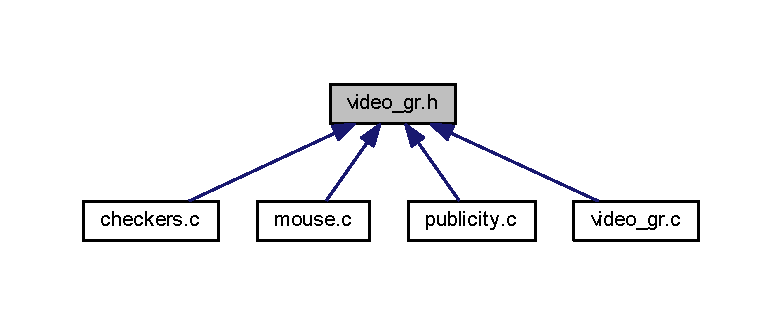
\includegraphics[width=350pt]{video__gr_8h__dep__incl}
\end{center}
\end{figure}
\subsection*{Functions}
\begin{DoxyCompactItemize}
\item 
unsigned \hyperlink{group__video__gr_ga80f6be1470280496d613f43fbf4f576c}{get\+Mouse\+\_\+buffer} ()
\begin{DoxyCompactList}\small\item\em gets pointer to variable mouse\+\_\+buffer \end{DoxyCompactList}\item 
unsigned \hyperlink{group__video__gr_gafa0e51016d7aa337778300ba2ec70a74}{get\+Double\+\_\+buffer} ()
\begin{DoxyCompactList}\small\item\em gets pointer to variable double\+\_\+buffer \end{DoxyCompactList}\item 
unsigned \hyperlink{group__video__gr_gae633b6fb3ed1e90fdcbc7b4c65ffe2ef}{get\+Video\+\_\+\+\_\+mem} ()
\begin{DoxyCompactList}\small\item\em gets pointer to variable video\+\_\+mem \end{DoxyCompactList}\item 
unsigned \hyperlink{group__video__gr_gaf597a67a797839097222fa9b4ae20b3f}{get\+H\+\_\+res} ()
\begin{DoxyCompactList}\small\item\em gets horizontal resolution of the screen \end{DoxyCompactList}\item 
unsigned \hyperlink{group__video__gr_ga36f1c43e43d903e085207548cf8d48a2}{get\+V\+\_\+res} ()
\begin{DoxyCompactList}\small\item\em gets vertical resolution of the screen \end{DoxyCompactList}\item 
void $\ast$ \hyperlink{group__video__gr_gacef21667c79365d57a084bed994c2189}{vg\+\_\+init} (unsigned short mode)
\begin{DoxyCompactList}\small\item\em Initializes the video module in graphics mode. \end{DoxyCompactList}\item 
int \hyperlink{group__video__gr_ga42f593e6656f1a978315aff02b1bcebf}{vg\+\_\+exit} (void)
\begin{DoxyCompactList}\small\item\em Returns to default Minix 3 text mode (0x03\+: 25 x 80, 16 colors) \end{DoxyCompactList}\item 
int \hyperlink{group__video__gr_ga729c07175ab64956c7fd9944d7676888}{vg\+\_\+set\+\_\+pixel} (int x, int y, unsigned int color)
\begin{DoxyCompactList}\small\item\em sets the color of a pixel in the double buffer and in the mouse buffer \end{DoxyCompactList}\item 
int \hyperlink{group__video__gr_ga78765c3e4634b79d0c27b464be410803}{vg\+\_\+set\+\_\+mouse\+\_\+pixel} (int x, int y, unsigned int color)
\begin{DoxyCompactList}\small\item\em sets the color of a pixel in the mouse buffer \end{DoxyCompactList}\item 
int \hyperlink{group__video__gr_gafcdcee0785e2e5a0d0f1f460bf436403}{vg\+\_\+draw\+\_\+square} (int xi, int yi, int size, int color)
\begin{DoxyCompactList}\small\item\em draws a square in the double buffer and in the mouse buffer \end{DoxyCompactList}\item 
int \hyperlink{group__video__gr_ga0410a09b926582249fb7c0a795c9d4fe}{vg\+\_\+draw\+\_\+circle} (int xi, int yi, int radius, int color)
\begin{DoxyCompactList}\small\item\em draws a circle in the double buffer and in the mouse buffer \end{DoxyCompactList}\item 
int \hyperlink{group__video__gr_gae50eb47e283e71498d323e815411acc3}{swap\+\_\+double\+\_\+video} ()
\begin{DoxyCompactList}\small\item\em copies the double\+\_\+buffer into the video\+\_\+buffer \end{DoxyCompactList}\item 
int \hyperlink{group__video__gr_ga8761e145d6f2249e0a4177ed7ff24299}{swap\+\_\+mouse\+\_\+video} ()
\begin{DoxyCompactList}\small\item\em copies the mouse\+\_\+buffer into the video\+\_\+buffer \end{DoxyCompactList}\item 
int \hyperlink{group__video__gr_ga56155e15f2cbeb0c0790c3b22db43a78}{swap\+\_\+mouse\+\_\+double} ()
\begin{DoxyCompactList}\small\item\em copies the mouse\+\_\+buffer into the double\+\_\+buffer \end{DoxyCompactList}\item 
int \hyperlink{group__video__gr_gacbc2b21e05ad693bb6ed614f87329f05}{swap\+\_\+double\+\_\+mouse} ()
\begin{DoxyCompactList}\small\item\em copies the double\+\_\+buffer into the mouse\+\_\+buffer \end{DoxyCompactList}\item 
int \hyperlink{group__video__gr_gaeae89e446fefdba5e72413ff38727f44}{mouse\+\_\+to\+\_\+double} (int x, int y)
\begin{DoxyCompactList}\small\item\em sets a pixel in the mouse buffer to the color of the corresponding pixel in the double buffer \end{DoxyCompactList}\end{DoxyCompactItemize}

%--- End generated contents ---

% Index
\backmatter
\newpage
\phantomsection
\clearemptydoublepage
\addcontentsline{toc}{chapter}{Index}
\printindex

\end{document}
